\documentclass[a4paper,oneside]{book}
%~~~~~~~~~ Document setup
\usepackage[spanish, mexico]{babel} % Formato en español
\usepackage[utf8]{inputenc} % Standard encoding
\usepackage{indentfirst} % Indents the first paragraph
\usepackage{amsmath} % Maths type package
\usepackage{bm} % Bold font maths
\usepackage{graphicx} % Advanced graphics package
\usepackage[export]{adjustbox} 
\usepackage{pdflscape} % Make pages landscape
\usepackage{fancyhdr} % Fancy headers
\usepackage[square,numbers]{natbib} % Bibliography los númeroes entre []
\usepackage{flafter} % Reference any 'float'
\usepackage[framemethod=tikz]{mdframed} % Box off stuff
\usepackage{wrapfig} % Text flowing around figures
\usepackage{lipsum} % Generates meaningless text
\usepackage{subfigure}
\usepackage{comment}

\usepackage{tabularx} % Para tablas que se ajustan al ancho de la página
\usepackage{booktabs} % Para un mejor formato de las líneas de la tabla
\usepackage{bigstrut}
\usepackage{colortbl}

% PARA TABLAS
\usepackage{longtable}
\usepackage{array}
\usepackage{multirow}
\usepackage{booktabs}

\usepackage{scalerel}

\pdfminorversion=7

% Define un nuevo tipo de columna "C" que centra el contenido y tiene un ancho fijo
\newcolumntype{C}[1]{>{\centering\arraybackslash}p{#1}}
\newcolumntype{M}[1]{>{\centering\arraybackslash}m{#1}}

% PARA COLOCARLA LA PALABRA CAPÍTULO A CADA \chapter
\usepackage{titletoc}%
\titlecontents{chapter}% <section-type>
  [0pt]% <left>
  {\bfseries}% <above-code>
  {\chaptername\ \thecontentslabel:\quad}% <numbered-entry-format>
  {}% <numberless-entry-format>
  {\hfill\contentspage}% <filler-page-format>

% IMPORTACIÓN DEL TEMPLATE
\usepackage{enumerate}
\usepackage[overload]{textcase}
\usepackage{times} % Cambia la fuente a Times New Roman
\usepackage{color}
\usepackage{algorithmicx,algpseudocode}
\usepackage{algorithm}
\usepackage{amsmath}
\usepackage{amssymb}
\usepackage{subfigure}
\usepackage{setspace}
\usepackage{float}
\usepackage{hyperref}
\usepackage{verbatim}
\usepackage{epstopdf}
\usepackage{ifpdf}
\usepackage{url}
\usepackage{multirow}
\usepackage{vmargin}
\usepackage{booktabs}
\usepackage{multirow}
\usepackage{rotating}

\urlstyle{same} %Hacer que la fuente del URL de la bibliografía sea la misma

\hypersetup{ %Color para los hiperenlaces
    colorlinks=true, % Sin recuadro en los links
    %colorlinks=false,
    citecolor=black, % Color del recuadro en los índices
    filecolor=black,
    linkcolor=black,
    urlcolor=black
}

% The following numbers determine the margins.
\setmarginsrb
{25mm}% left margin (Estaba en 35)
{25mm}% top margin
{25mm}% right margin
{20mm}% bottom margin
{0mm}{0mm}{0mm}{10mm}% not needed -- related to headers and footers

% Tamaño de la fuente del documento
\usepackage{scrextend}
\usepackage{anyfontsize}
\changefontsizes{11 pt}

% Valor del  espacio del interlineado
\renewcommand{\baselinestretch}{1.3}

% INFORMACIÓN DEL DOCUMENTO
% \def\documenttitle {LOREM IPSUM DOLOR SIT AMET, CONSECTETUR ADIPISCING ELIT. SED VARIUS}

\def\documenttitle {DISEÑO DE UN SISTEMA INTEGRADO PARA EL CONTROL DE CALIDAD DE PRENDAS DE VESTIR}

% \def\documentsubtitle {Plan de Tesis para optar el Título de Ingeniero Mecatrónico}

\def\documentsubtitle {1MTR01 Trabajo de Fin de Carrera 1}
\def\documentauthor {Alibert Luna Palomino}
\def\myadvisor{José Mauricio Díaz Jurado}
\def\mycoadvisor{-}
\def\universityname {PONTIFICIA UNIVERSIDAD CATÓLICA DEL PERÚ}
\def\universityfaculty {FACULTAD DE CIENCIAS E INGENIERÍA}
\def\universityimage {img/logo_PUCP_antiguo.pdf}
\def\universitylocation{Lima}
\def\documentdate {\today}


% Definición del nuevo comando
% #1 es el parámetro que representa la ruta de la imagen
\newcommand{\IMM}[3]{
	\adjustbox{margin=#3}{\includegraphics[width=#1\textwidth]{#2}}
}

% Comando para escalar objetos
\newcommand{\B}[2]{\scaleobj{#2}{#1}}

\def\anchoFPT{10em}
\def\anchoFP{8em}
\def\OpR{$\color{red}\B{\blacklozenge}{1.35}$}
\def\OpA{$\color{blue}\B{\blacklozenge}{1.35}$}
\def\OpV{$\color[HTML]{4CD514}{\B{\blacklozenge}{1.35}}$}
\def\OpN{$\color{orange}\B{\blacklozenge}{1.35}$}

% ---------- INICIO DE PÁGINAS ----------
\pagestyle{empty} % Quitar footers y headers
\begin{document}

% PORTADA
%\makeatletter
\begin{titlepage}
\centering
%%% Caratula

%%%% Cabecera
\vskip 2.5cm
\Large\textbf{\universityname}\\
\bigskip
\large\textbf{\universityfaculty}

%%%% Logo de la PUCP
\vskip 1.0cm
\includegraphics[scale=1.0]{\universityimage}

%%%% Titulo de la Tesis:
\vskip 0.5cm
\large\textbf{\documenttitle}

%%%% Datos del Tesista:
\vskip 1cm
\large\textbf{\documentsubtitle}
\vskip 1cm
\Large\textbf{AUTOR:}\\  \documentauthor

%%%% Datos del Asesor:
\vskip 2cm
\Large\textbf{ASESOR:}\\  \myadvisor \\
%\Large\textbf{CO-ASESOR:}\\  \mycoadvisor
\vskip 1.5cm
%%%% Lugar y fecha:
\vskip 3cm
\large \universitylocation, \documentdate

\end{titlepage}

% RESUMEN
%\chapter*{Resumen}
%\addcontentsline{toc}{chapter}{Resumen}

\clearpage

% AGRADECIMIENTOS
% \thispagestyle{empty} %Removes the page numbering.
    \null\vspace{\stretch {1}}
        \begin{flushright}
                A mis padres por su incondicional apoyo durante todos estos años de carrera.
                
                A mi familia por la confianza depositada en mi.
                
                A mi asesor por ayudarme y orientarme en el desarrollo de esta tesis.
                
                A mis amigos por acompañarme durante toda esta experiencia.
        \end{flushright}
\vspace{\stretch{2}}\null

% ÍNDICE
\tableofcontents

% LISTA DE FIGURAS
%\renewcommand\listfigurename{\centering Índice de Figuras}
\listoffigures
\clearpage

%LISTA DE TABLAS
%\renewcommand\listtablename{\centering Índice de Tablas}
\listoftables
\clearpage

%CONTENIDO
%% % PARA HACER QUE LA INTRODUCCIÓN NO TENGA NÚMERO
% \chapter*{Introducción}
% % PARA HACER QUE LA INTRODUCCIÓN APAREZCA EN EL ÍNDICE COMO CHAPTER
% \addcontentsline{toc}{chapter}{Introducción}

\chapter{Introducción}
\section{Problemática}

El presente proyecto aborda su problemática central a través de tres enfoques interrelacionados: primero, se destaca la importancia del control de calidad dentro de la industria de la moda; en segundo lugar, se identifican las ineficiencias inherentes al control de calidad tradicional; y finalmente, se subraya la creciente necesidad de automatización en el proceso de control de calidad.

\subsection*{Importancia del Control de Calidad en la Industria de la Moda}

Entre enero y mayo de 2022, las exportaciones de camisas, pantalones y camisetas en Perú experimentaron incrementos notables, con crecimientos del 57\%, 49\% y 31\% en valor, respectivamente. Hasta mayo de 2022, las exportaciones de confecciones alcanzaron los 759 millones de dólares americanos, marcando un aumento del 36\% en comparación con el año anterior \cite{LaCamara2022}. Estas estadísticas demuestran un crecimiento significativo en la exportación de prendas de vestir peruanas, por lo cual, es importante mantener altos estándares de calidad para satisfacer las expectativas de mercados internacionales exigentes.

\begin{figure}[H]
	\centering
	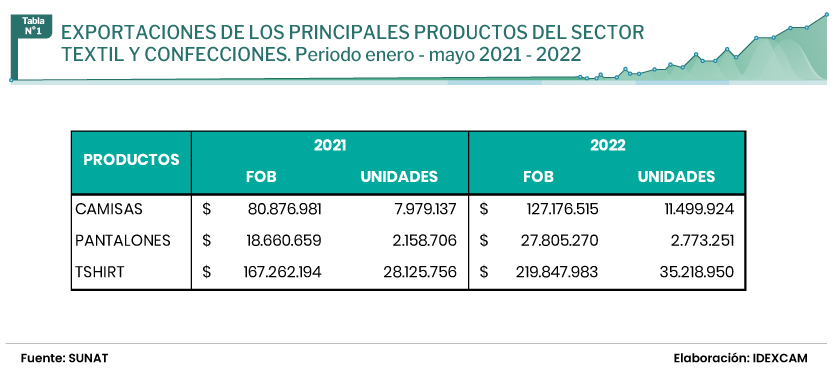
\includegraphics[width=0.8\textwidth]{img/exportaciones.jpg}
	\caption[Exportaciones peruanas de textiles: aumento en FOB y unidades, 2021 vs 2022.]{Exportaciones peruanas de textiles: aumento en FOB y unidades, 2021 vs 2022. Fuente \cite{LaCamara2022}.}
\end{figure}

El control de calidad en la industria textil es esencial para asegurar que las prendas no solo cumplan con los estándares de calidad establecidos, sino también que ofrezcan seguridad y durabilidad. Este proceso minucioso abarca diversas etapas, incluyendo la inspección de tejidos, la graduación de patrones, el corte, la costura, el acabado y finalmente, el empaquetado. Todo ello con el objetivo de garantizar que el producto final cumpla con las expectativas de los clientes. Entre los defectos más comunes que se identifican durante estas etapas se encuentran las variaciones de color, manchas, agujeros, puntadas rotas, costuras desalineadas, hilos sueltos, así como medidas incorrectas y tallas inconsistentes, tanto en los tejidos como en la construcción de las prendas \cite{TetraInspection2024}. 

\subsection*{Ineficiencias en el Control de Calidad Tradicional}

El enfoque tradicional de control de calidad, que se centra principalmente en inspecciones al final del proceso y en la implementación de correcciones a posterior, resulta en elevados costos debido a desechos y reparaciones. Este enfoque repercute negativamente en la competitividad y sostenibilidad de las empresas. Un estudio realizado por \cite{BonillaPastor2015} sobre la gestión de calidad en micro y pequeñas empresas (Mypes) del sector textil en Perú, destaca las graves consecuencias económicas y ambientales que surgen de una gestión de calidad ineficaz. Desde el punto de vista económico, los residuos y desperdicios producidos por procesos ineficientes constituyen un gasto promedio del 7.4\% en relación con el costo total de producción, lo cual impacta directamente en la competitividad y la rentabilidad de las empresas.

El control de calidad manual, como se observa en la Figura \ref{fig:insp_manual}, es ampliamente utilizada en procesos de producción debido a su relativa facilidad y la no necesidad de equipos técnicos especializados. Sin embargo, enfrenta desafíos significativos debido a factores humanos como los que se detallan en la Tabla \ref{tab:eficiencia_inspección}. Dichos factores inciden directamenteb en la efectividad del control de calidad manual, elevando potencialmente la incidencia de errores en la evaluación de la calidad. Investigaciones referenciadas en el estudio de \cite{KujawinskaVogt2015} revelan que, en tareas de inspección simples, la tasa de error puede fluctuar entre un 3\% y un 30\%, dependiendo de la índole de la tarea y las condiciones en que se efectúa la inspección.

\begin{figure}[H]
	\centering
	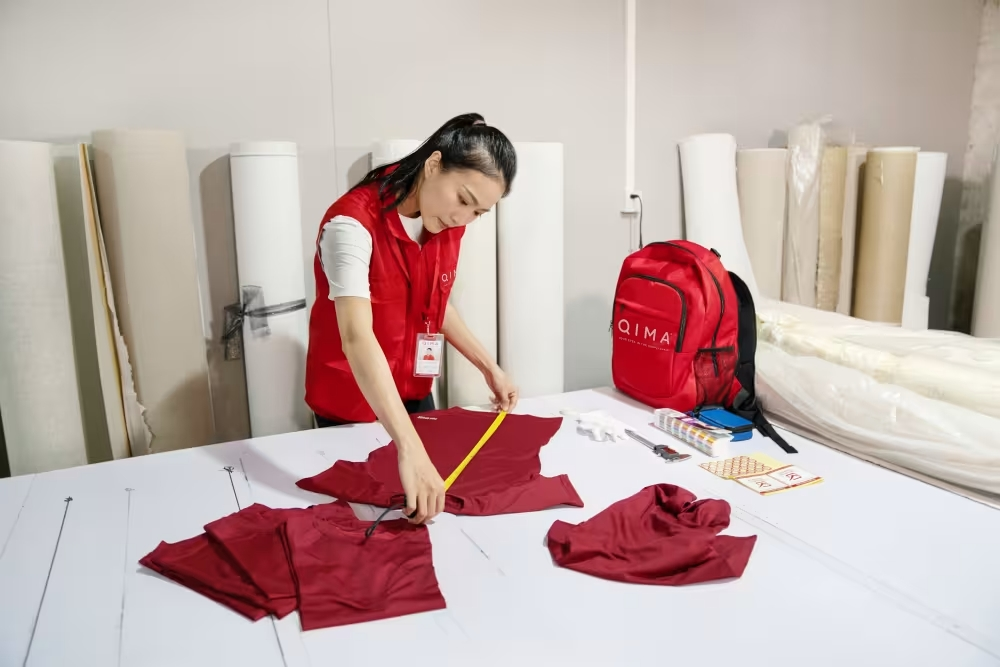
\includegraphics[width=0.65\textwidth]{img/insp_manual.jpg}
	\caption[Inspección manual de prendas de vestir.]{Inspección manual de prendas de vestir. Fuente: \cite{qimaProcedimientosInspeccin}.}
	\label{fig:insp_manual}
\end{figure}

\begin{table}[H]
	\centering
	\caption[Factores que afectan la eficiencia de la inspección visual.]{Factores que afectan la eficiencia de la inspección visual. Fuente: \cite{KujawinskaVogt2015}.}
	\begin{tabular}{|p{10em}|p{18em}|}
		\hline
		\textbf{Factors} & \textbf{Examples} \bigstrut\\
		\hline
		Technical & {Type of defects; Defect visibility; Quality level; Standards (tests); Control automation;  Other} \bigstrut\\
		\hline
		Psychophysical & Age;  Sex;  Observation  skills;  Experience;  Temperament;  Creativity;  Other \bigstrut\\
		\hline
		Organizational & Training;  Scope  of  decision  making; Feedback;  Precise  instructions;  Other \bigstrut\\
		\hline
		Workplace environment & {Light; Noise; Temperature; Work time; Workstation organization; Other} \bigstrut\\
		\hline
		Social & {Team communication;  Pressure;  Isolation; Other} \bigstrut\\
		\hline
	\end{tabular}%
	\label{tab:eficiencia_inspección}%
\end{table}%

\subsection*{Necesidad de Mejora y Automatización}

La integración de la Inteligencia Artificial (IA) en el control de calidad de la industria textil y de la moda ha introducido métodos avanzados para la inspección de calidad, desde la producción hasta la revisión final de las prendas. Esta innovación mejora significativamente la eficiencia y precisión, minimizando los errores humanos y los costos de producción, mientras asegura la adherencia a estándares de calidad elevados \cite{TextileLearner}. La Tabla \ref{tab:visual_vs_automated} resume la comparación entre inspección visual humana y la inspección automatizada. Estas limitaciones subrayan la necesidad de un proceso de inspección más automatizado y preciso para reducir errores y mejorar la eficiencia \cite{Islam2006ASuitable}.

\begin{table}[H]
	\centering
	\caption[Inspección visual versus inspección automatizada.]{Inspección visual versus inspección automatizada \cite{Islam2006ASuitable}.}
	\begin{tabular}{|p{13em}|c|c|}
		\hline
		\textbf{Inspection Type} & {\textbf{Visual}} & \textbf{Automated} \bigstrut\\
		\hline
		Fabric Types & 100\% & \multicolumn{1}{c|}{70\%} \bigstrut\\
		\hline
		Defect Detection Rate & 70\%  & 80\%+ \bigstrut\\
		\hline
		Reproducibility & 50\%  & 90\%+ \bigstrut\\
		\hline
		Objective Defect Judgment & 50\%  & {100\%} \bigstrut\\
		\hline
		Statistics Ability & 0\%   & 95\%+ \bigstrut\\
		\hline
		Inspection Speed & {30 m/min} & {120 m/min} \bigstrut\\
		\hline
		Response Type & 50\%  & {80\%} \bigstrut\\
		\hline
		Information Content & 50\%  & 90\%+ \bigstrut\\
		\hline
		Information Exchange & 20\%  & 90\%+ \bigstrut\\
		\hline
	\end{tabular}%
	\label{tab:visual_vs_automated}%
\end{table}%

La automatización en la detección de defectos mediante visión artificial es crucial en manufactura, mejorando la consistencia y reduciendo errores humanos. La inspección óptica automatizada, impulsada por aprendizaje profundo y machine learning, supera los métodos manuales, ofreciendo eficiencia y precisión. Esto facilita la identificación rápida y confiable de defectos, elevando la calidad del producto y disminuyendo costos y tiempos de producción. La utilización de redes neuronales convolucionales para la extracción de características mejora la adaptabilidad y eficiencia de la inspección, siendo clave para el avance en manufactura. \cite{SanchezRomero2023}.

\section{Propuesta de Solución}

\section{Objetivos}

El proyecto presenta un objetivo general del cual surgen \ref{lst:objetivos_especificos} objetivos específicos para lograr el cumplimiento del objetivo general.

\subsection{Objetivo General}

Desarrollar un sistema integrado para el control de calidad de prendas de vestir, que combine tecnologías de visión artificial y detección de metales para inspeccionar cada prenda de manera individual, asegurando su conformidad con los estándares de calidad establecidos en la ficha técnica de la prenda, tales como la ausencia de defectos visibles, la precisión en las medidas de talla y la detección de elementos metálicos extraños.

\subsection{Objetivos Específicos}

\begin{enumerate}
\setlength\itemsep{-0.5em}
    \item Realizar una revisión bibliográfica (estado del arte) que permita definir los requerimientos del diseño del sistema y todo lo concerniente al diseño conceptual.
    
    \item Definir las exigencias específicas que debe cumplir el sistema para lograr el objetivo principal.
      
    \item Seguir la metodología de diseño basada en la norma VDI 2206 para el diseño mecatrónico completo del sistema.
        
    \item Diseñar un subsistema mecánico que permita transportar las prendas de vestir a través de los distintos módulos del sistema.
    
    \item Diseñar un subsistema de inspección por visión artificial para el control de defectos en prendas de vestir.
    
    \item Diseñar un subsistema de inspección por procesamiento de imágenes para realizar la medición de la talla de las prendas y realizar la verificación según la ficha técnica de la prenda.
    
    \item Diseñar un subsistema de detección de metales que examine cada prenda para identificar y alertar sobre la presencia de agujas, alfileres o cualquier otro elemento metálico extraño, garantizando así la seguridad del producto final.
    
    \item Desarrollar una interfaz intuitiva para mostrar resultados de detección de calidad de prendas, incluyendo visualización de defectos, mediciones de tallas e identificación de metales
    
    \item Seleccionar el concepto de solución óptimo basados en los criterios técnicos y económicos, según la norma VDI 2225.
    
    \item Estimar un costo de fabricación de un prototipo a partir de los componentes seleccionados.
    
    \label{lst:objetivos_especificos}
\end{enumerate}

\section{Metodología}
% BENDEZU_LEDESMA_JORGE_DISEÑO_PROTOTIPO_DRON

Para el desarrollo del presente trabajo se emplearan adaptaciones de las metodologías diseñadas por la VDI (Asociación Alemana de Ingenieros). Entre ellas, se utilizar una adaptación de la metodología VDI 2206 \cite{VDIVDE2206_2021} y de la metodología VDI 2221 \cite{VDI2221_2019} para el diseño conceptual, el cual consistirá en las siguientes etapas: Elaboración de lista de requerimientos, Elaboración de un diagrama de funciones y Elaboración de una matriz morfológica (con 3 soluciones). Posteriormente se seguirá una adaptación de la metodología VDI 2225 \cite{VDI2225_series} para realizar un análisis técnico y económica de las soluciones.

De ese modo, los Capítulos 1 y 2 se enfocaran en a comprender la problemática de la investigación. El Capítulo 1 aborda una investigación preliminar para contextualizar el problema, identificar los enfoques de la problemática y definir el alcance de la solución. El Capítulo 2, por su parte, examina el estado actual de la tecnología para establecer un marco de referencia que permita evaluar la viabilidad del proyecto, con el fin de determinar parámetros y características relevantes para el sistema de control de calidad en prendas de vestir.

En el Capítulo 3, se desarrollan los procesos de la metodología correspondientes para diseñar la estructura de funciones y el concepto de solución. Utilizando la lista de requerimientos, se abstrae el problema para obtener una comprensión amplia de las funciones necesarias, lo que guía el diseño mecánico y eléctrico inicial y ayuda a determinar los sensores, actuadores y fuentes de energía necesarios. A partir de esta estructura, se crea una matriz morfológica que facilita la combinación de distintas alternativas de solución, culminando en la definición precisa de los objetivos de diseño e implementación. Además, se realizará una ponderación de los conceptos de solución a través de un análisis técnico-económico con el objetivo de obtener un concepto de solución óptimo.

Por último, en los capítulos subsecuentes se realizaran los siguientes partes del trabajo:

\begin{itemize}
	\setlength\itemsep{-0.5em}
	\item Realización de cálculos mecánicos, electrónicos y de control necesarios para determinar las características de la máquina.
	\item Se va a seleccionar (o diseñar) un modelo de inteligencia artificial para realizar la labor de la visión artificial del sistema, además, se va a buscar, o en su defecto, se va a crear un dataset para entrenar un modelo de inteligencia artificial.
	\item Verificación de las partes mecánicas por medio de software de elementos finitos.
	\item Elaboración de planos y estimación de costos de fabricación.
\end{itemize}

\section{Alcance de la Investigación}

Este trabajo se centra en el diseño de un sistema mediante el dimensionamiento detallado de cada uno de sus componentes, con el objetivo de que opere de forma completamente autónoma. Esto significa que la única interacción humana necesaria será la inserción de la prenda a verificar, el ingreso de señales de control y posteriormente, la retirada de la prenda ya evaluada. Es importante destacar que los requisitos definidos para este proyecto, desarrollados a lo largo de la investigación, están orientados a un entorno no industrial. Además, se señala que el prototipo busca alcanzar un Nivel 4 de Madurez Tecnológica (TRL4), mediante simulaciones que se llevarán a cabo tanto en software como a través de un Producto Mínimo Viable (MVP) en un entorno de laboratorio controlado.

Para concluir, esta tesis presentará todos los cálculos de diseño necesarios, así como los planos mecánicos y electrónicos, los materiales escogidos para el proyecto, y los diagramas de flujo que explican la operación y control del sistema.

\chapter{Estado del Arte}
\label{Estado del Arte}
En este capítulo se presenta una revisión de trabajos de investigación, sistemas comerciales y patentes relacionados al control de calidad automático de prendas de vestir. Asimismo, se presentan las tecnologías involucradas a la detección de defectos mediante visión artificial, detección de metales, y luz UV para detectar manchas de grasa en las prendas de vestir.

% \section{Sistema Integrado de Control de Calidad de Prendas}

\subsection{Investigaciones Académicas}

\subsubsection{System of error detection in the manufacture of garments using artificial vision}

El sistema desarrollado la investigación \cite{Moreno2017} consiste en un sistema de visión artificial implementado para detectar errores en la etapa de corte durante el proceso de fabricación de prendas en la industria textil. Utiliza un sistema embebido Raspberry Pi 3, equipado con el sistema operativo basado en Linux Raspbian y el compilador OpenCV para el desarrollo de códigos de visión por computadora. Este sistema, que se muestra en \ref{fig:luz_sistema}, logra segmentar perfectamente las prendas independientemente del color que se les haya dado en procesos anteriores, gracias a la implementación de un fondo dinámico opaco compuesto por LEDs RGB que cambian de color dependiendo del contraste con la prenda.

El algoritmo principal del sistema inicia con la captura de la imagen de la prenda, seguido por el promedio de cada canal de la imagen completa (rojo, verde y azul). Luego, se cambia el color del fondo basándose en el color que menos presencia tenga en la imagen, utilizando combinaciones de colores primarios en los LEDs RGB para minimizar el consumo de corriente. Finalmente, se captura una nueva imagen con el fondo bien contrastado con la prenda para verificar el contraste correcto.

\begin{figure}[H]
	\centering
	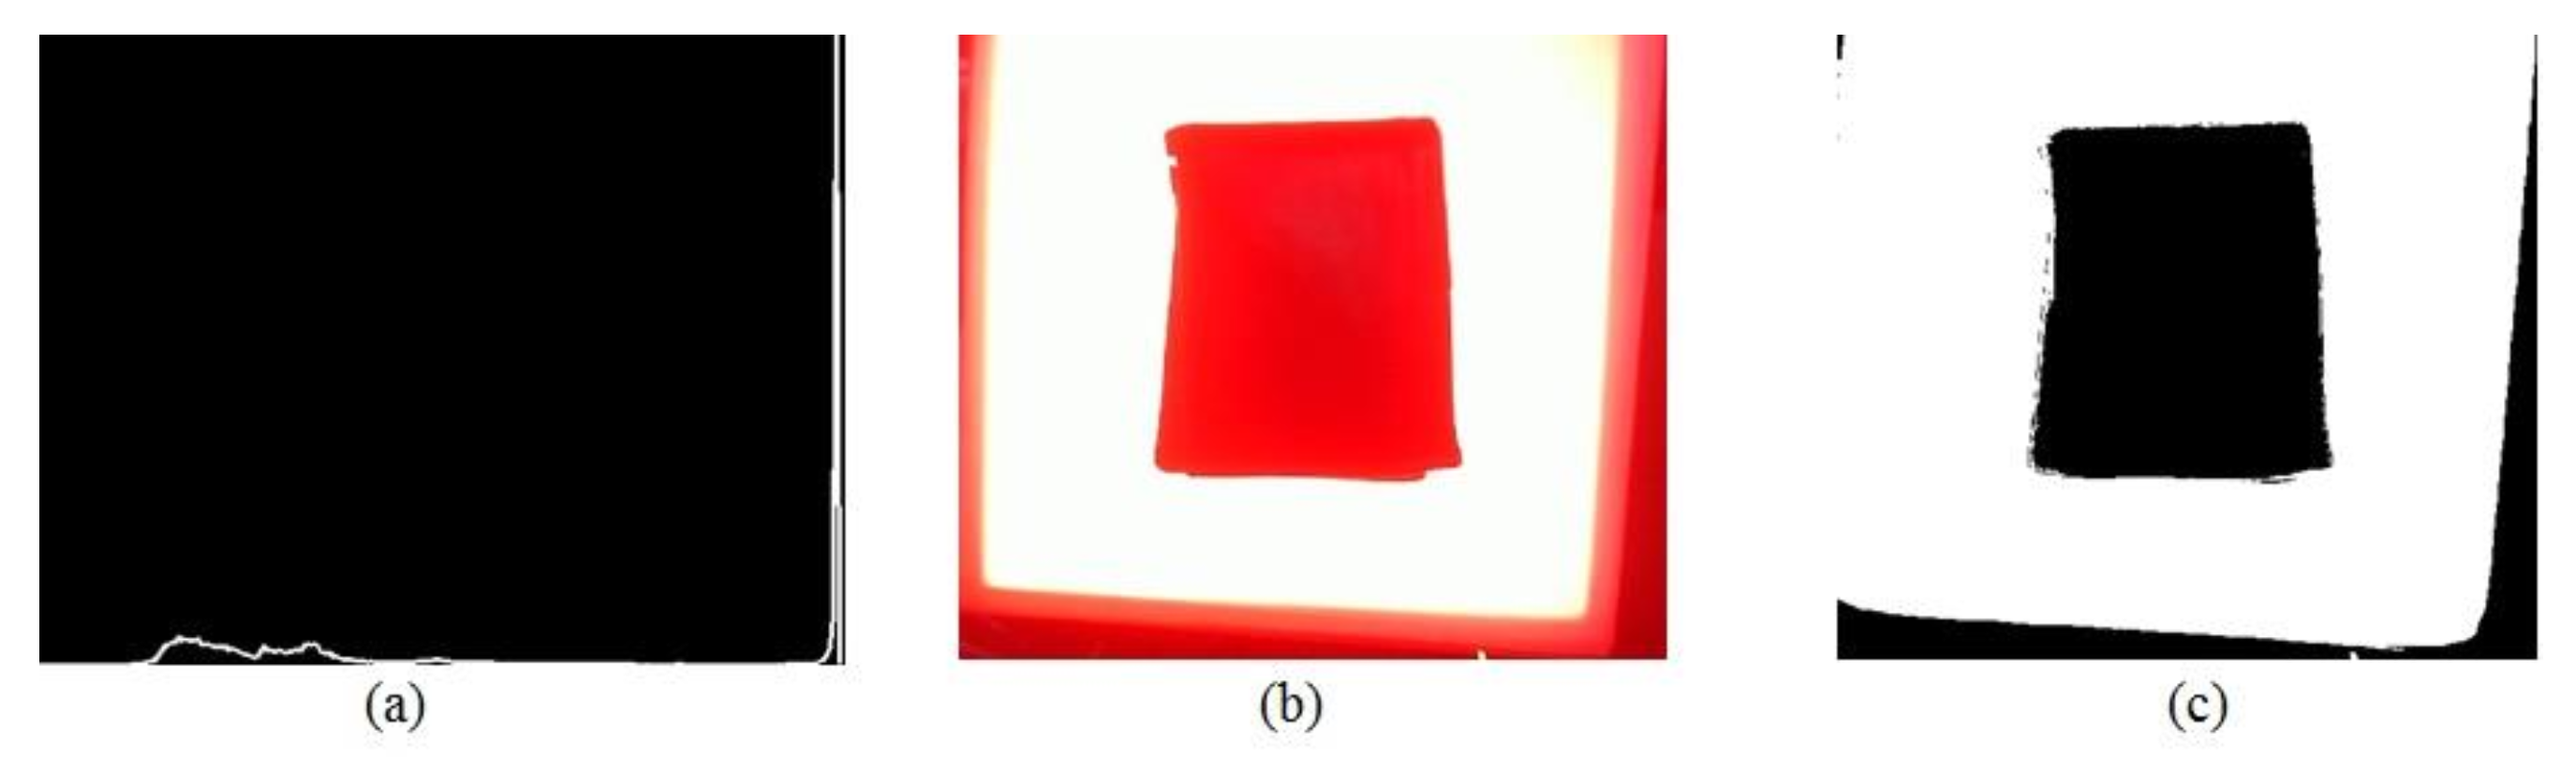
\includegraphics[width=0.8\textwidth]{img/luz_sistema.png}
	\caption[Sistema de visión artificial con fondo dinámico.]{Sistema de visión artificial con fondo dinámico \cite{Moreno2017}.}
	\label{fig:luz_sistema}
\end{figure}

\subsubsection{Using object detection technology to identify defects in clothing for blind people}

En la investigación \cite{Rocha2023} se muestra como la tecnología de detección de objetos, específicamente la arquitectura You Only Look Once (YOLO), ha sido aplicada de manera innovadora para ayudar a las personas ciegas a identificar defectos, como manchas o agujeros, en su ropa. Este enfoque utiliza un sistema de detección de defectos basado en el aprendizaje profundo para categorizar y detectar estas imperfecciones en prendas de vestir, lo que representa un paso importante hacia la mejora de la autonomía y la confianza de las personas ciegas en la selección de su vestimenta. El sistema propuesto en este estudio se basa en la recolección de un conjunto de datos específico de ropa con defectos, el cual es utilizado para entrenar y evaluar el sistema. La metodología empleada para optimizar el sistema de detección de defectos incluye aumentar el conjunto de datos con nuevos defectos, condiciones de iluminación y fondos, introducir la ampliación de datos y la clasificación de defectos, demostrando ser eficaz y adecuado para diferentes condiciones de detección de defectos desafiantes.

El trabajo futuro en este campo se centra en la creación de una aplicación móvil y un sistema mecatrónico, como un armario automático, que incorpore los algoritmos y metodologías desarrolladas. Esto no solo pone de manifiesto la utilidad práctica de la tecnología de detección de objetos para la comunidad ciega, sino que también abre la puerta a aplicaciones automáticas que pueden facilitar aún más la gestión del vestuario por parte de las personas con discapacidad visual, proporcionando una herramienta de apoyo esencial para su independencia y confianza en la vida cotidiana. Este enfoque innovador destaca el potencial de las tecnologías de visión por computadora en la asistencia y mejora de la calidad de vida de las personas con discapacidades visuales.

\begin{figure}[H]
	\centering
	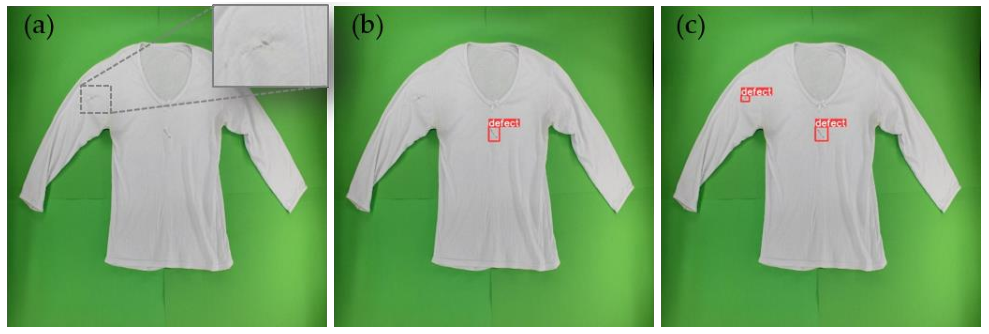
\includegraphics[width=0.9\textwidth]{img/example_YOLO.pdf}
	\caption[Defecto ignorado por YOLOv5m6, detectado tras la ampliación de datos.]{Defecto ignorado por YOLOv5m6, detectado tras la ampliación de datos desarrolada por \cite{Rocha2023}: (a) imagen original, (b) imagen predicha por el modelo YOLOv5m6 sin ampliación, y (c) imagen predicha por el modelo YOLOv5m6 con ampliación.}
	\label{fig:example_YOLO}
\end{figure}

\subsubsection{Automatic Measurement of Garment Sizes Using Image Recognition}

El documento presenta una innovadora metodología para medir automáticamente las tallas de prendas de vestir utilizando tecnología de reconocimiento de imágenes mediante el dispositivo que se muestra en la Figura \ref{fig:Automatic_Measurement}. Al enfrentar el problema de altas tasas de devolución en la moda en línea, debido a las inconsistencias en las tallas entre diferentes marcas y fabricantes, este estudio propone una solución tecnológica que combina el diseño de un conjunto de equipos especializados para capturar imágenes de prendas extendidas y un enfoque de medición automática basado en plantillas de prendas. Estas plantillas permiten identificar el tipo de prenda y puntos de características clave para calcular sus tallas. Este método ofrece una herramienta útil y eficiente para la medición de prendas, mostrando resultados precisos que satisfacen los requisitos de la industria del vestido, y tiene el potencial de mejorar significativamente la experiencia de compra en línea al reducir la tasa de devoluciones gracias a una estandarización en la medición de tallas \cite{Li2017AutomaticMeasurement}.

\begin{figure}[H]
	\centering
	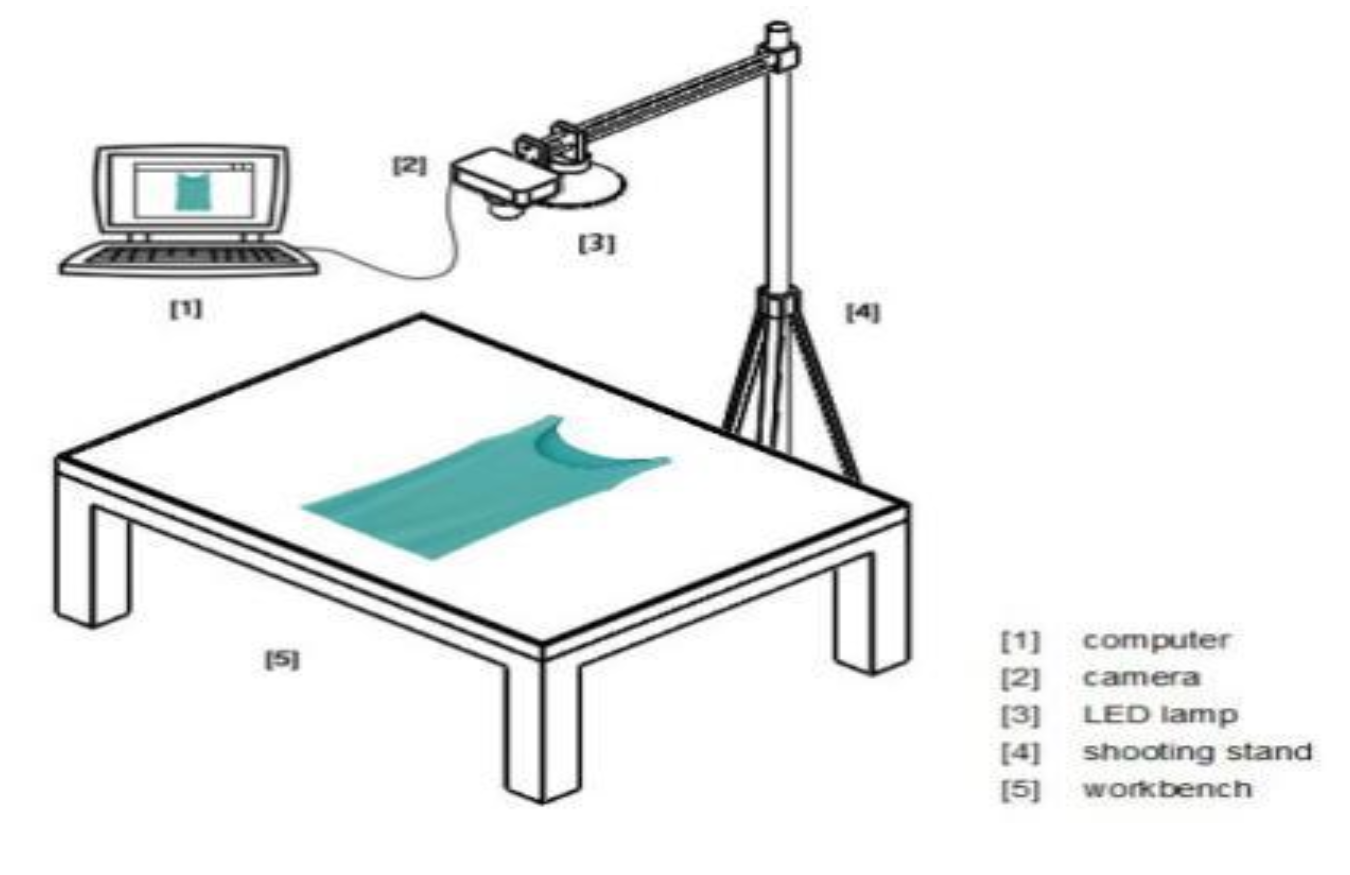
\includegraphics[width=0.6\textwidth]{img/Automatic_Measurement.png}
	\caption[Diseño de un dispositivo para medición automática de tallas de prendas mediante reconocimiento de imágenes]{Diseño de un dispositivo para medición automática de tallas de prendas mediante reconocimiento de imágenes \cite{Li2017AutomaticMeasurement}.}
	\label{fig:Automatic_Measurement}
\end{figure}

\subsection{Productos Comerciales}

\subsubsection{Handheld Needle Detector ON-30}

En el contexto de la detección de metales en la industria textil, el Detector de Agujas Portátil ON-30 de Oshima, que se muestra en la Figura \ref{fig:oshima_on_30} se presenta como una herramienta eficaz. Este dispositivo, alimentado por baterías AA y basado en inducción magnética, se destaca por su capacidad para identificar con precisión objetos metálicos pequeños. Su diseño compacto y la implementación de alarmas visuales y sonoras facilitan su uso en diversas situaciones, ofreciendo una solución práctica para garantizar la seguridad en los procesos de producción textil \cite{oshimaEfficientHandheld}. Las características de este producto se observan en el Cuadro \ref{tab:specs_ON_30}.

\begin{figure}[H]
	\centering
	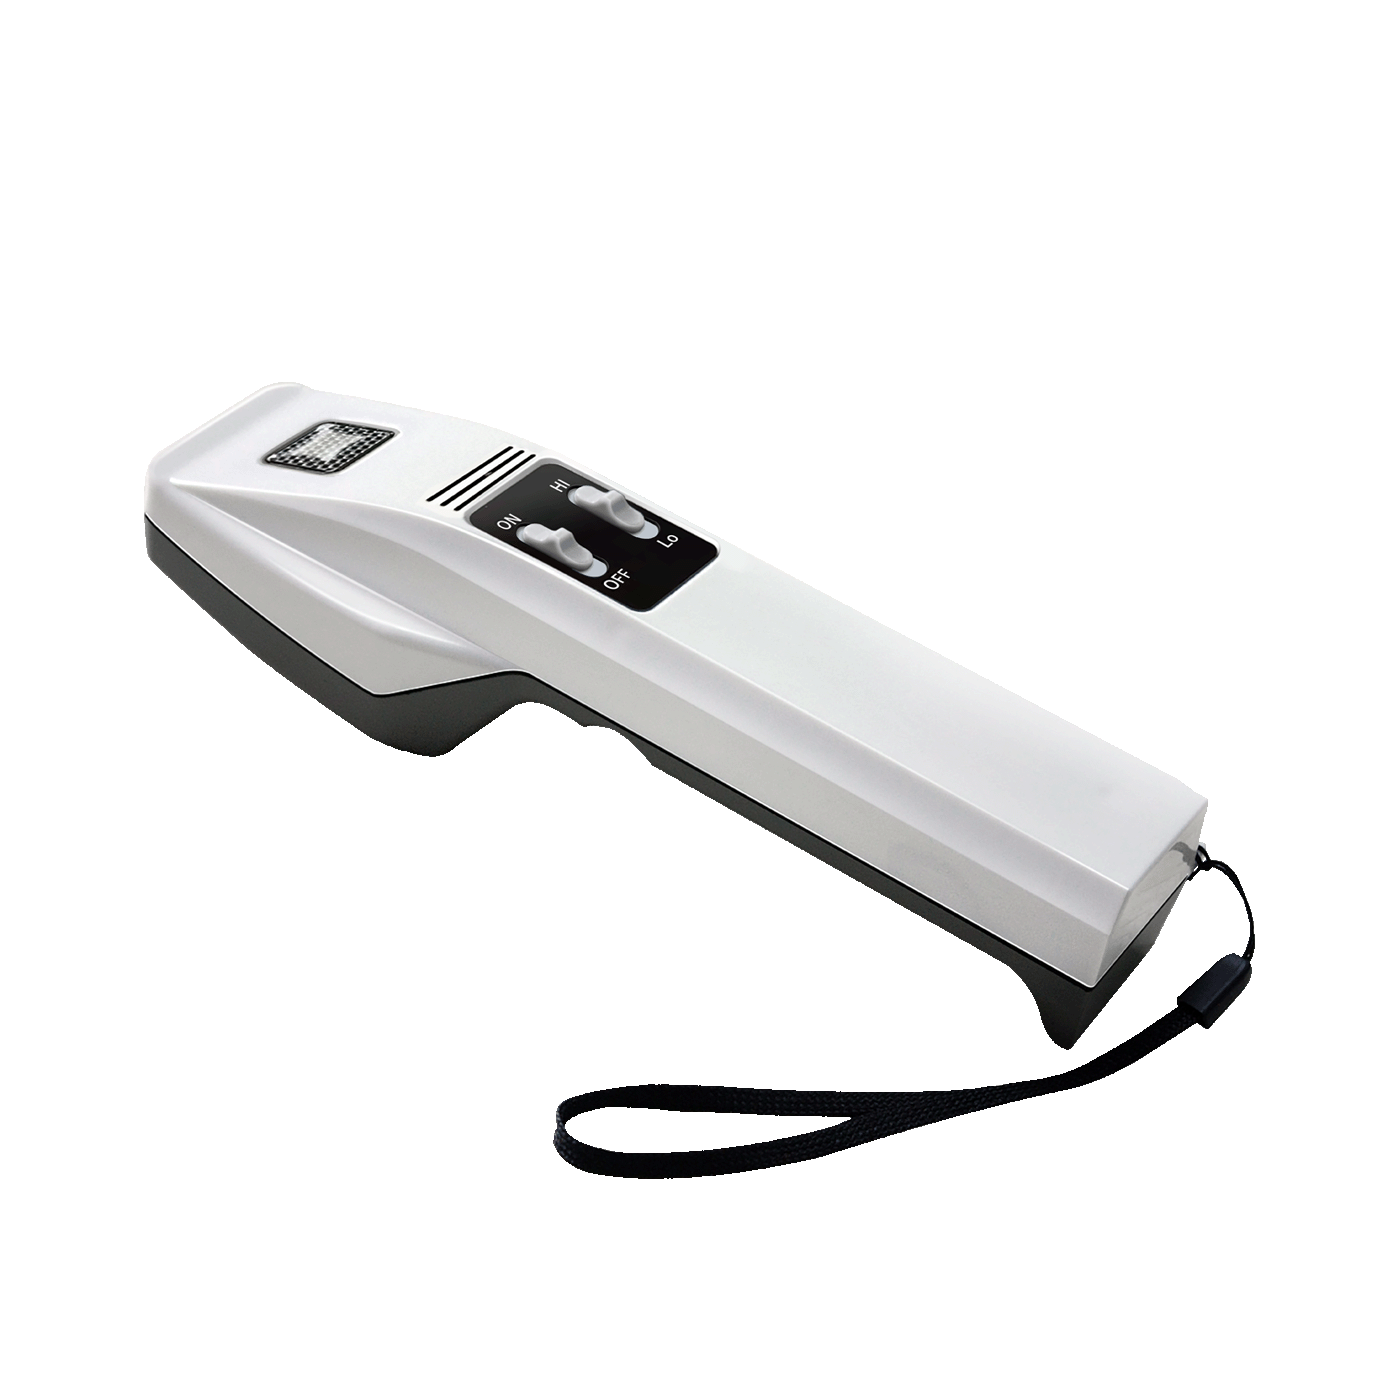
\includegraphics[width=0.4\textwidth]{img/oshima_on_30.png}
	\caption{Detector de Agujas Portátil ON-30 de Oshima.}
	\label{fig:oshima_on_30}
\end{figure}

\begin{table}[H]
	\caption{Especificaciones del Modelo ON-30.}
	\begin{tabularx}{\textwidth}{|l|X|}
		\hline
		\textbf{Característica} & \textbf{Especificación} \\ \hline
		Modelo & ON-30 \\ \hline
		Fuente de Alimentación & Batería 6F22-9V, corriente de reposo del LED <5mA. Alarma de sonido y luz. Corriente dinámica <30mA, corriente dinámica de la alarma de vibración <60mA, ahorro de energía. \\ \hline
		Sensibilidad & La inspección cercana puede detectar una bola de hierro de 0.5 mm, una bola de hierro de 1.2 mm de diámetro hasta una altura de 10 mm. La máxima sensibilidad puede detectar una bola de hierro de 0.8 mm de diámetro, un pasador de ruptura de 0.7 x 20 de diámetro hasta una altura de 50 mm. \\ \hline
		Método de Detección & Inducción magnética \\ \hline
		Espacio de Detección (mm) & 70x55 \\ \hline
		Alarma & Zumbador, lámpara \\ \hline
		Dimensiones LxAxA (mm) & 195x58x50 \\ \hline
		Volumen del Empaque LxAxA (mm) & 250x100x55 \\ \hline
		Peso Neto/Peso Bruto (kg) & 0.212/0.35 \\ \hline
	\end{tabularx}
	\label{tab:specs_ON_30}
\end{table}

\subsubsection{Digital Conveyor Needle Detectors ON-688CD6S/688CDD6S}

Los detectores de agujas para cinta transportadora ON-688CD6S/688CDD6S de OSHIMA incorporan sensores de 10 puntos para una mayor sensibilidad y confiabilidad, con ajuste de sensibilidad en tres niveles para diferentes necesidades de detección. Su interfaz de pantalla táctil facilita su uso, y la máquina es capaz de conectarse a datos, contabilizar productos, y calibrarse automáticamente cada dos horas \cite{oshimaOSHIMAGarment}. Las especificaciones de estos modelos se muestran en la Tabla \ref{tab:specs_ON-688CD6S/688CDD6S}.

\begin{figure}[H]
	\centering
	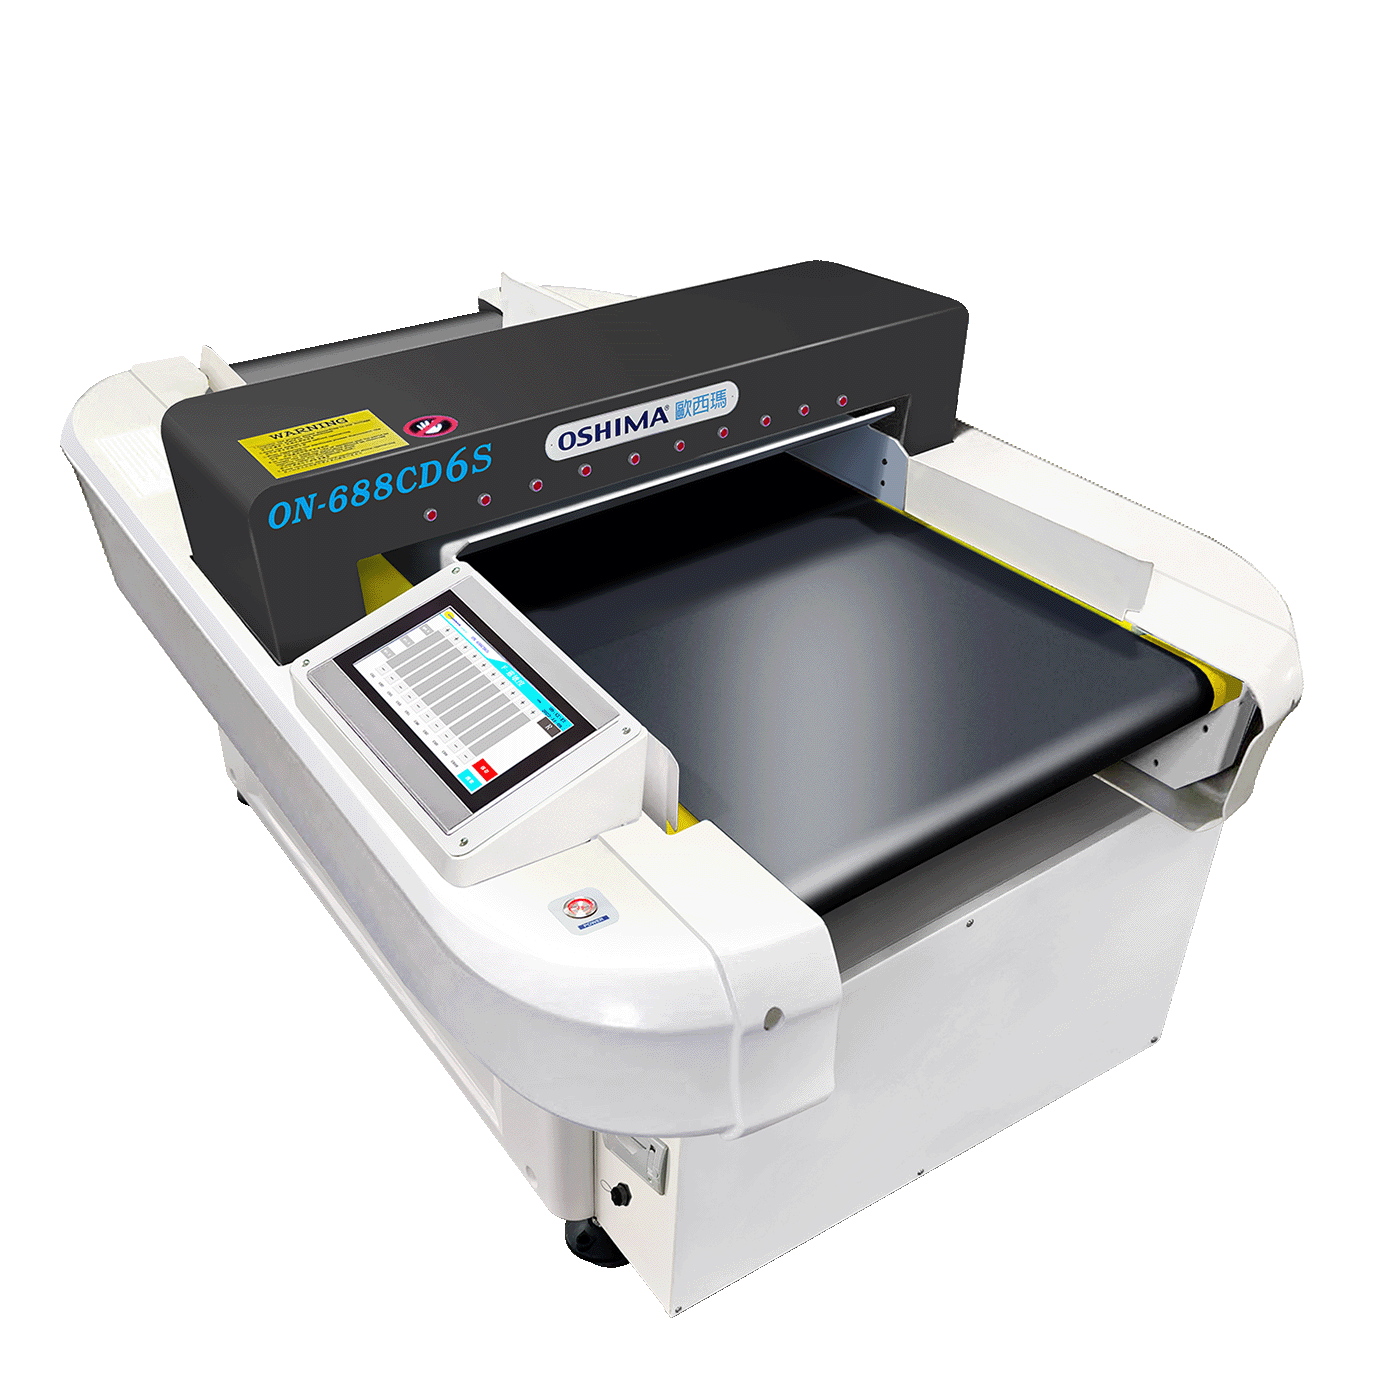
\includegraphics[width=0.5\textwidth]{img/oshima_conveyor.png}
	\caption{Detectores de Agujas para Cinta Transportadora Digital ON-688CD6S/688CDD6S.}
	\label{fig:oshima_conveyor}
\end{figure}

\begin{table}[H]
	\caption{Especificaciones de los modelos ON-688CD6S/688CDD6S.}
	\begin{tabularx}{\textwidth}{|X|X|X|}
		\hline
		\multirow{2}{*}[2pt]{\textbf{Característica}} & \multicolumn{2}{c|}{\textbf{Especificaciones}} \\ \cline{2-3}
		& \textbf{ON-688CD6S} & \textbf{ON-688CDD6S} \\
		\hline
		Detecting tower & Single tower & Double tower \\
		\hline
		Detective height (mm) & 100 & 100 \\
		\hline
		Detective width (mm) & 600 & 600 \\
		\hline
		Effective detecting Height (mm) & 90 & 90 \\
		\hline
		Power supply & 1P AC220V 50/60Hz & 1P AC220V 50/60Hz \\
		\hline
		Rate (kW) & 0.2 & 0.2 \\
		\hline
		Detective capability of iron ball (mm) & Fe 0.8/1.0/1.2 & Fe 0.8/1.0/1.2 \\
		\hline
		Sensitivity adjustment & Level adjustment & Level adjustment \\
		\hline
		Conveyor speed (m/min) & 32 & 32 \\
		\hline
		Detection method & Magnet & Magnet \\
		\hline
		Alarm & Automatic buzzer and alarm indicator light, the conveyor rewinding function & Automatic buzzer and alarm indicator light, the conveyor rewinding function \\
		\hline
		Dimensions LxWxH (mm) & 1720X1100X920 & 1820X1180X1100 \\
		\hline
		Packaging volume LxWxH (mm) & 2160X1060X920 & 2330X1130X1100 \\
		\hline
		N.W/G.W (kg) & 280/380 & 420/570 \\
		\hline
	\end{tabularx}
	\label{tab:specs_ON-688CD6S/688CDD6S}
\end{table}

\subsubsection{AI-Driven Measurement Checking Machine}

Este desarrollo tecnológico, el cual se muestra en la Figura \ref{fig:inspection_machine} de la empresa Dongguan Yunji Zhihui Technology facilita la automatización de procesos previamente manuales, por lo que augura reducciones significativas en los costos laborales y mejoras en el control de calidad \cite{RMG2021AIGarment}. Las especificaciones de este sistema se muestran en la Tabla \ref{tab:spec_inspection_machine}.

\begin{figure}[H]
	\centering
	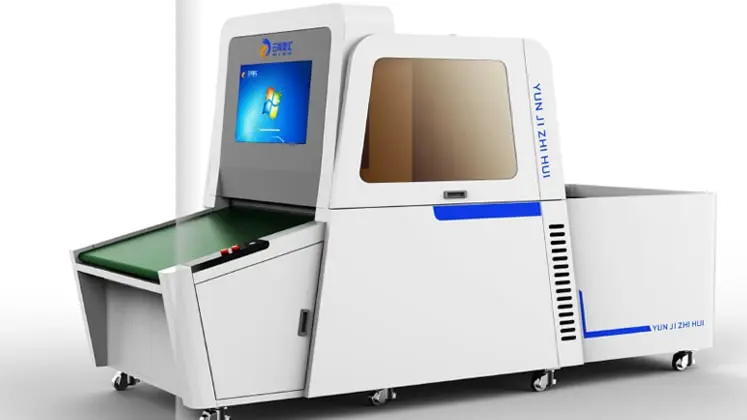
\includegraphics[width=0.7\textwidth]{img/inspection_machine.png}
	\caption[Máquina de chequeo de medidas conducido por IA.]{Máquina de chequeo de medidas conducido por IA. Fuente: \cite{RMG2021AIGarment}.}
	\label{fig:inspection_machine}
\end{figure}

\begin{table}[h!]
	\centering
	\caption[Características cuantitativas del sistema de inspección de prendas con IA.]{Características cuantitativas del sistema de inspección de prendas con IA. Fuente: Elaboración propia.}
	\begin{tabular}{|l|l|}
		\hline
		\textbf{Característica} & \textbf{Valor} \\ \hline
		Dimensiones medidas por prenda & 15 dimensiones \\ \hline
		Tiempo por artículo & Máximo 6 segundos \\ \hline
		Capacidad de procesamiento & 4800 camisetas en 480 minutos \\ \hline
		Precisión de medición & Error dentro de ±1 mm \\ \hline
		Exactitud de detección & Hasta el 99.5\% \\ \hline
		Adaptabilidad & Ajuste según color y tela de las prendas \\ \hline
	\end{tabular}
	\label{tab:spec_inspection_machine}
\end{table}

\subsection{Patentes}

\subsubsection{US20200178632A1}
La invención \cite{us20200178632a1} describe un aparato, método y sistema de control automatizado para mejorar la inspección, medición y fabricación de prendas de vestir como se observa en la Figura \ref{fig:US20200178632A1-20200611-D00005}. Este sistema captura una imagen de la prenda la convierte en una representación digital que puede enviarse y almacenarse en una base de datos. Esta información digital se utiliza para recrear prendas ideales con medidas y patrones reproducibles. Además, el sistema permite comparaciones con imágenes ideales existentes y/o con la propia prenda para determinar si posee las dimensiones, formas, colores, texturas y tejidos correctos.

\begin{figure}[H]
    \centering
    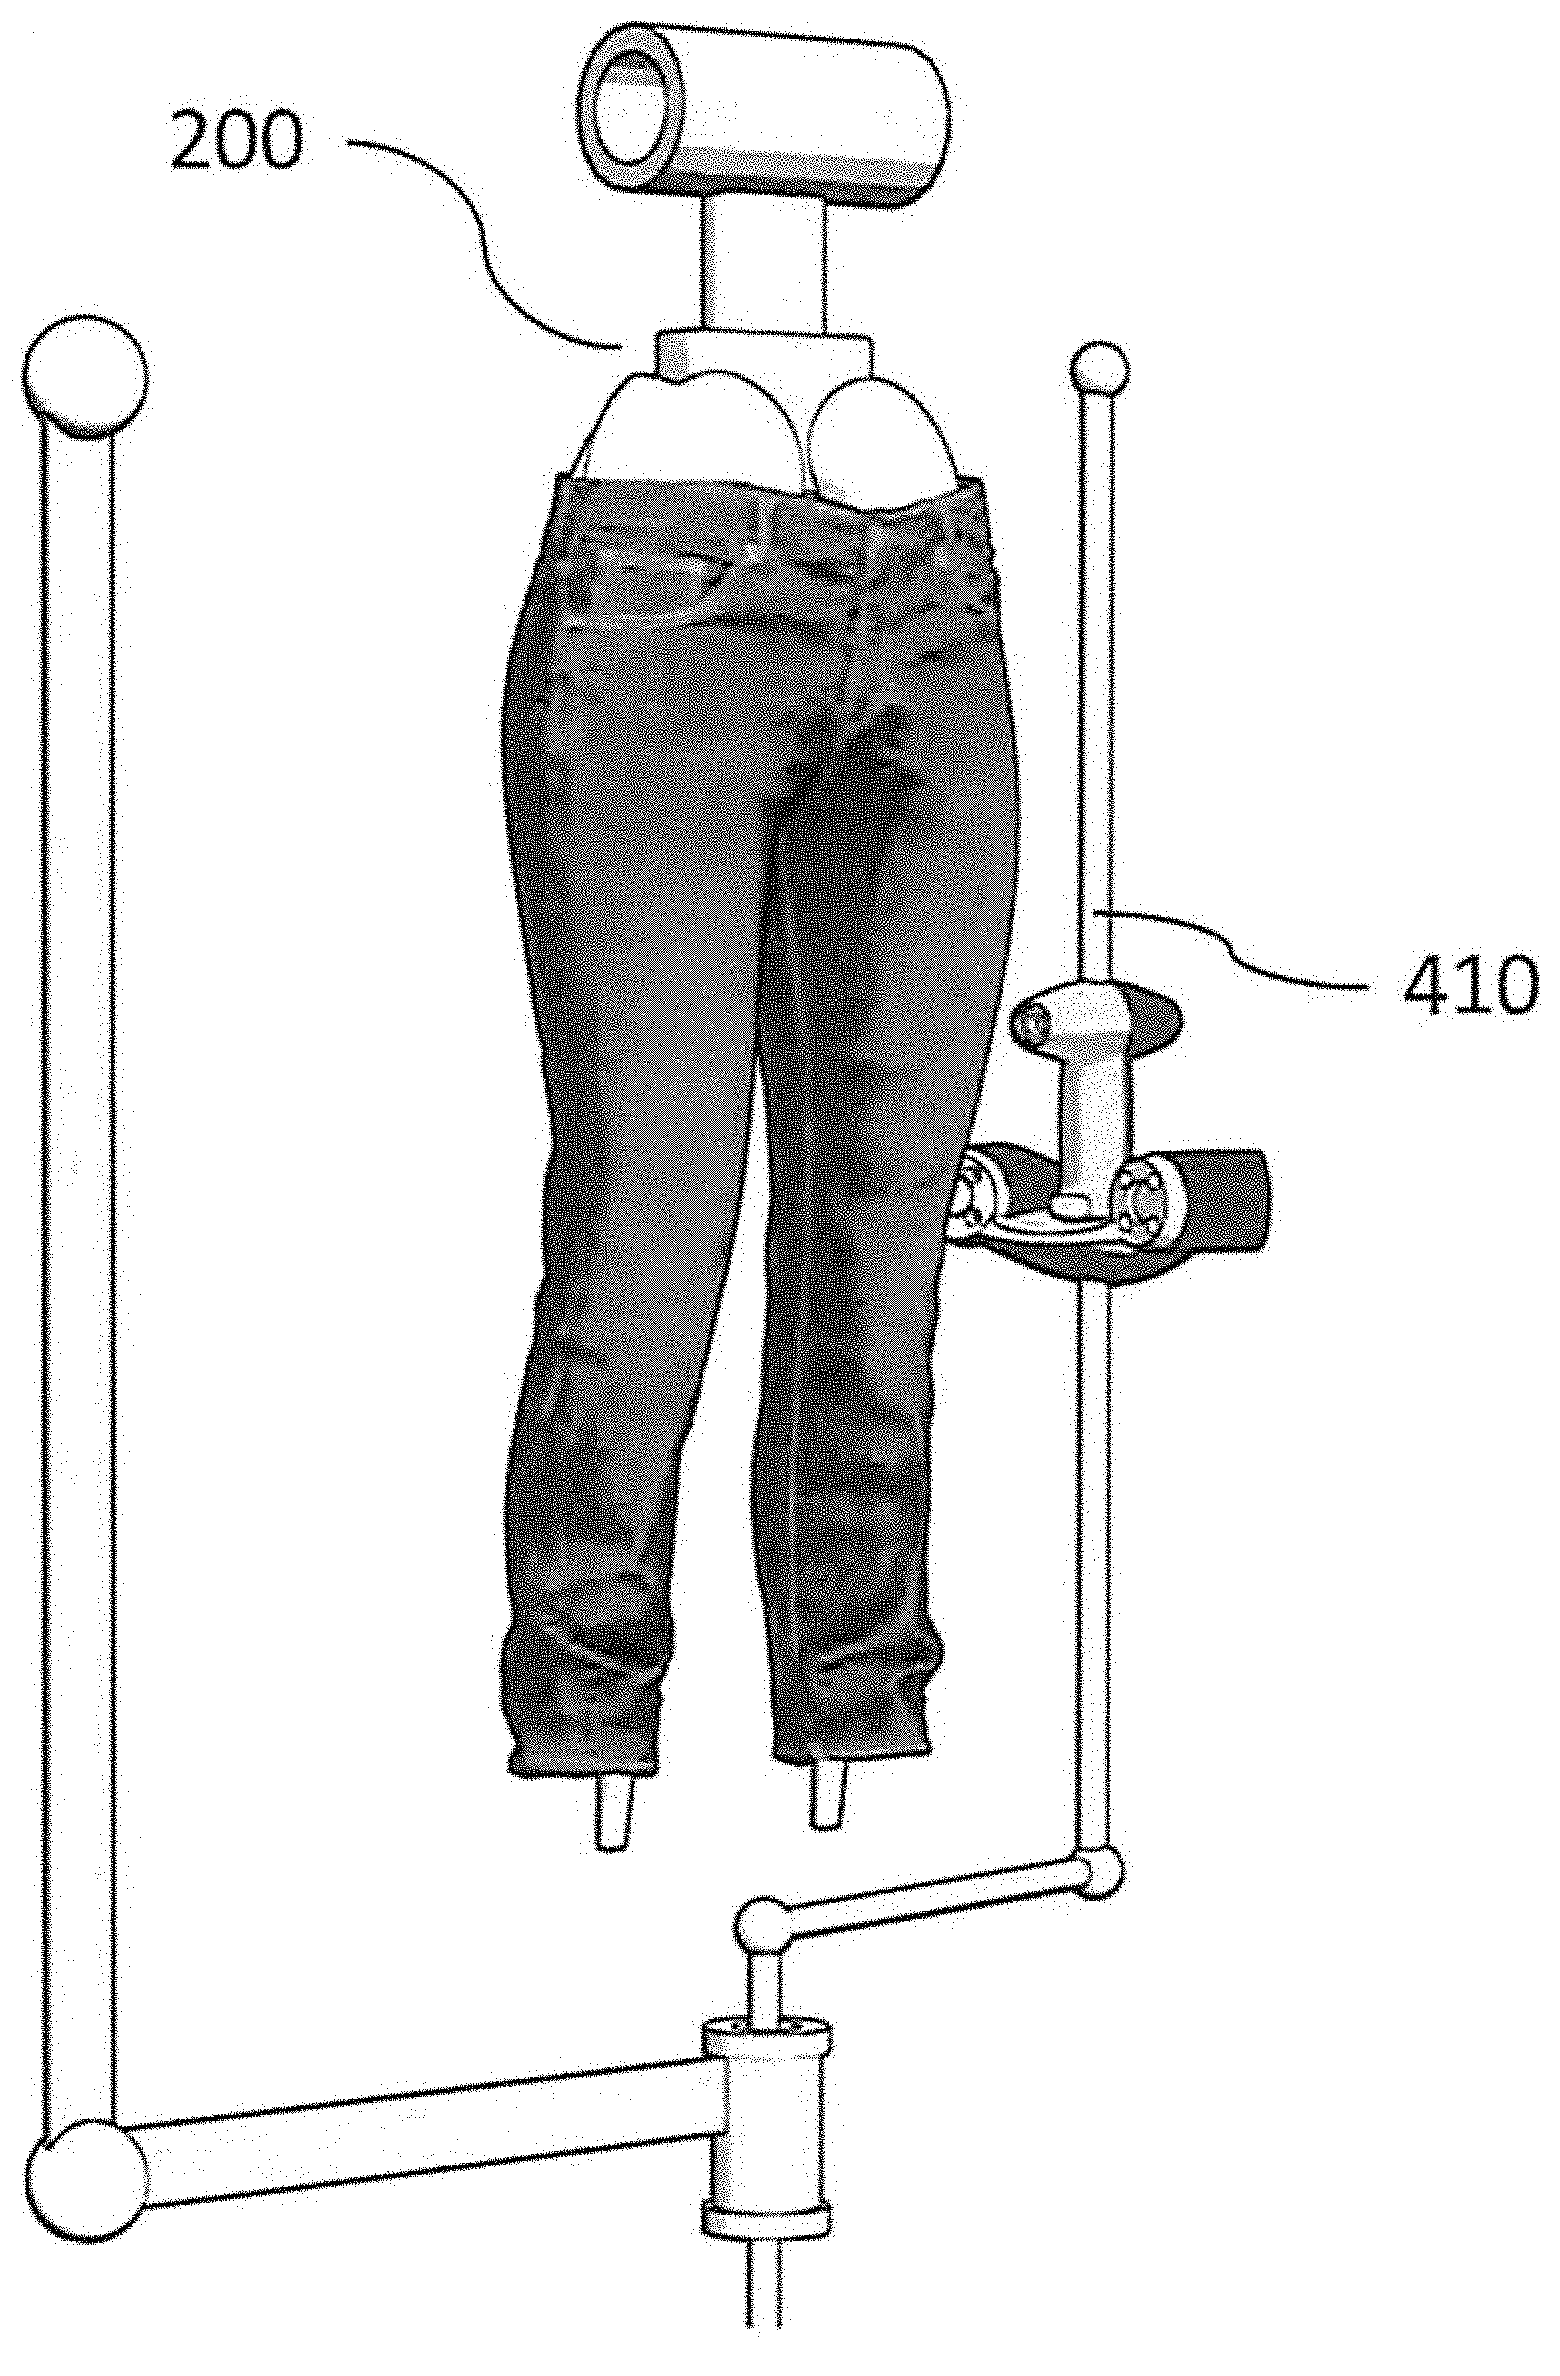
\includegraphics[width=0.3\textwidth]{img/US20200178632A1-20200611-D00005.png}
    \caption{Patente con captura de detalles en 3D.}
    \label{fig:US20200178632A1-20200611-D00005}
\end{figure}

\subsubsection{US5530652A}

La invención \cite{US5530652A} detalla un sistema que incluye técnicas de escaneo 3D (ópticas o electroópticas) para adquirir datos de escaneo dimensionales. Estos datos se procesan para la extracción de medidas y retroalimentación. La organización de los datos permite su almacenamiento y recuperación, finalizando con el control de medidas de las prendas, la fabricación y la categorización basada en la retroalimentación.

Este sistema se destaca por su capacidad para automatizar el control y la inspección de la calidad de las prendas producidas, minimizando la necesidad de contacto humano directo con los objetos, lo que facilita un análisis dimensional preciso y automatizado. La tecnología descrita en esta patente tiene potencial para revolucionar la forma en que se miden, inspeccionan y fabrican las prendas de vestir, asegurando consistencia y calidad en la producción de vestimenta.

La patente US5530652 describe un sistema automático de inspección y medición de prendas que puede crear representaciones electrónicas bidimensionales o tridimensionales de un objeto. Estas representaciones pueden ser combinadas con otras para crear una base de datos de medidas de donde se pueden generar patrones estándar para su uso en la fabricación de prendas. Además, la representación electrónica puede utilizarse para comparar el objeto fabricado con una representación ideal, determinando si las medidas del objeto se encuentran dentro de una tolerancia predeterminada respecto a la representación ideal. Se emplea un sistema de visión por máquina para capturar una imagen del objeto y convertirla en una representación digital, que luego puede agregarse a una base de datos para compilar un patrón ideal o compararse con una imagen ideal existente para verificar si el objeto tiene el tamaño correcto.

La patente aborda el desarrollo de un método y un sistema para la inspección y medición automática de prendas, con el objetivo de asegurar que las dimensiones de las prendas fabricadas se ajusten a los estándares ideales y tolerancias predefinidas. Esto facilita la creación de bases de datos de medidas que pueden utilizarse para mejorar la fabricación de prendas, asegurando una mayor precisión y consistencia en el tamaño y la calidad de las prendas producidas.

\begin{figure}[H]
	\centering
	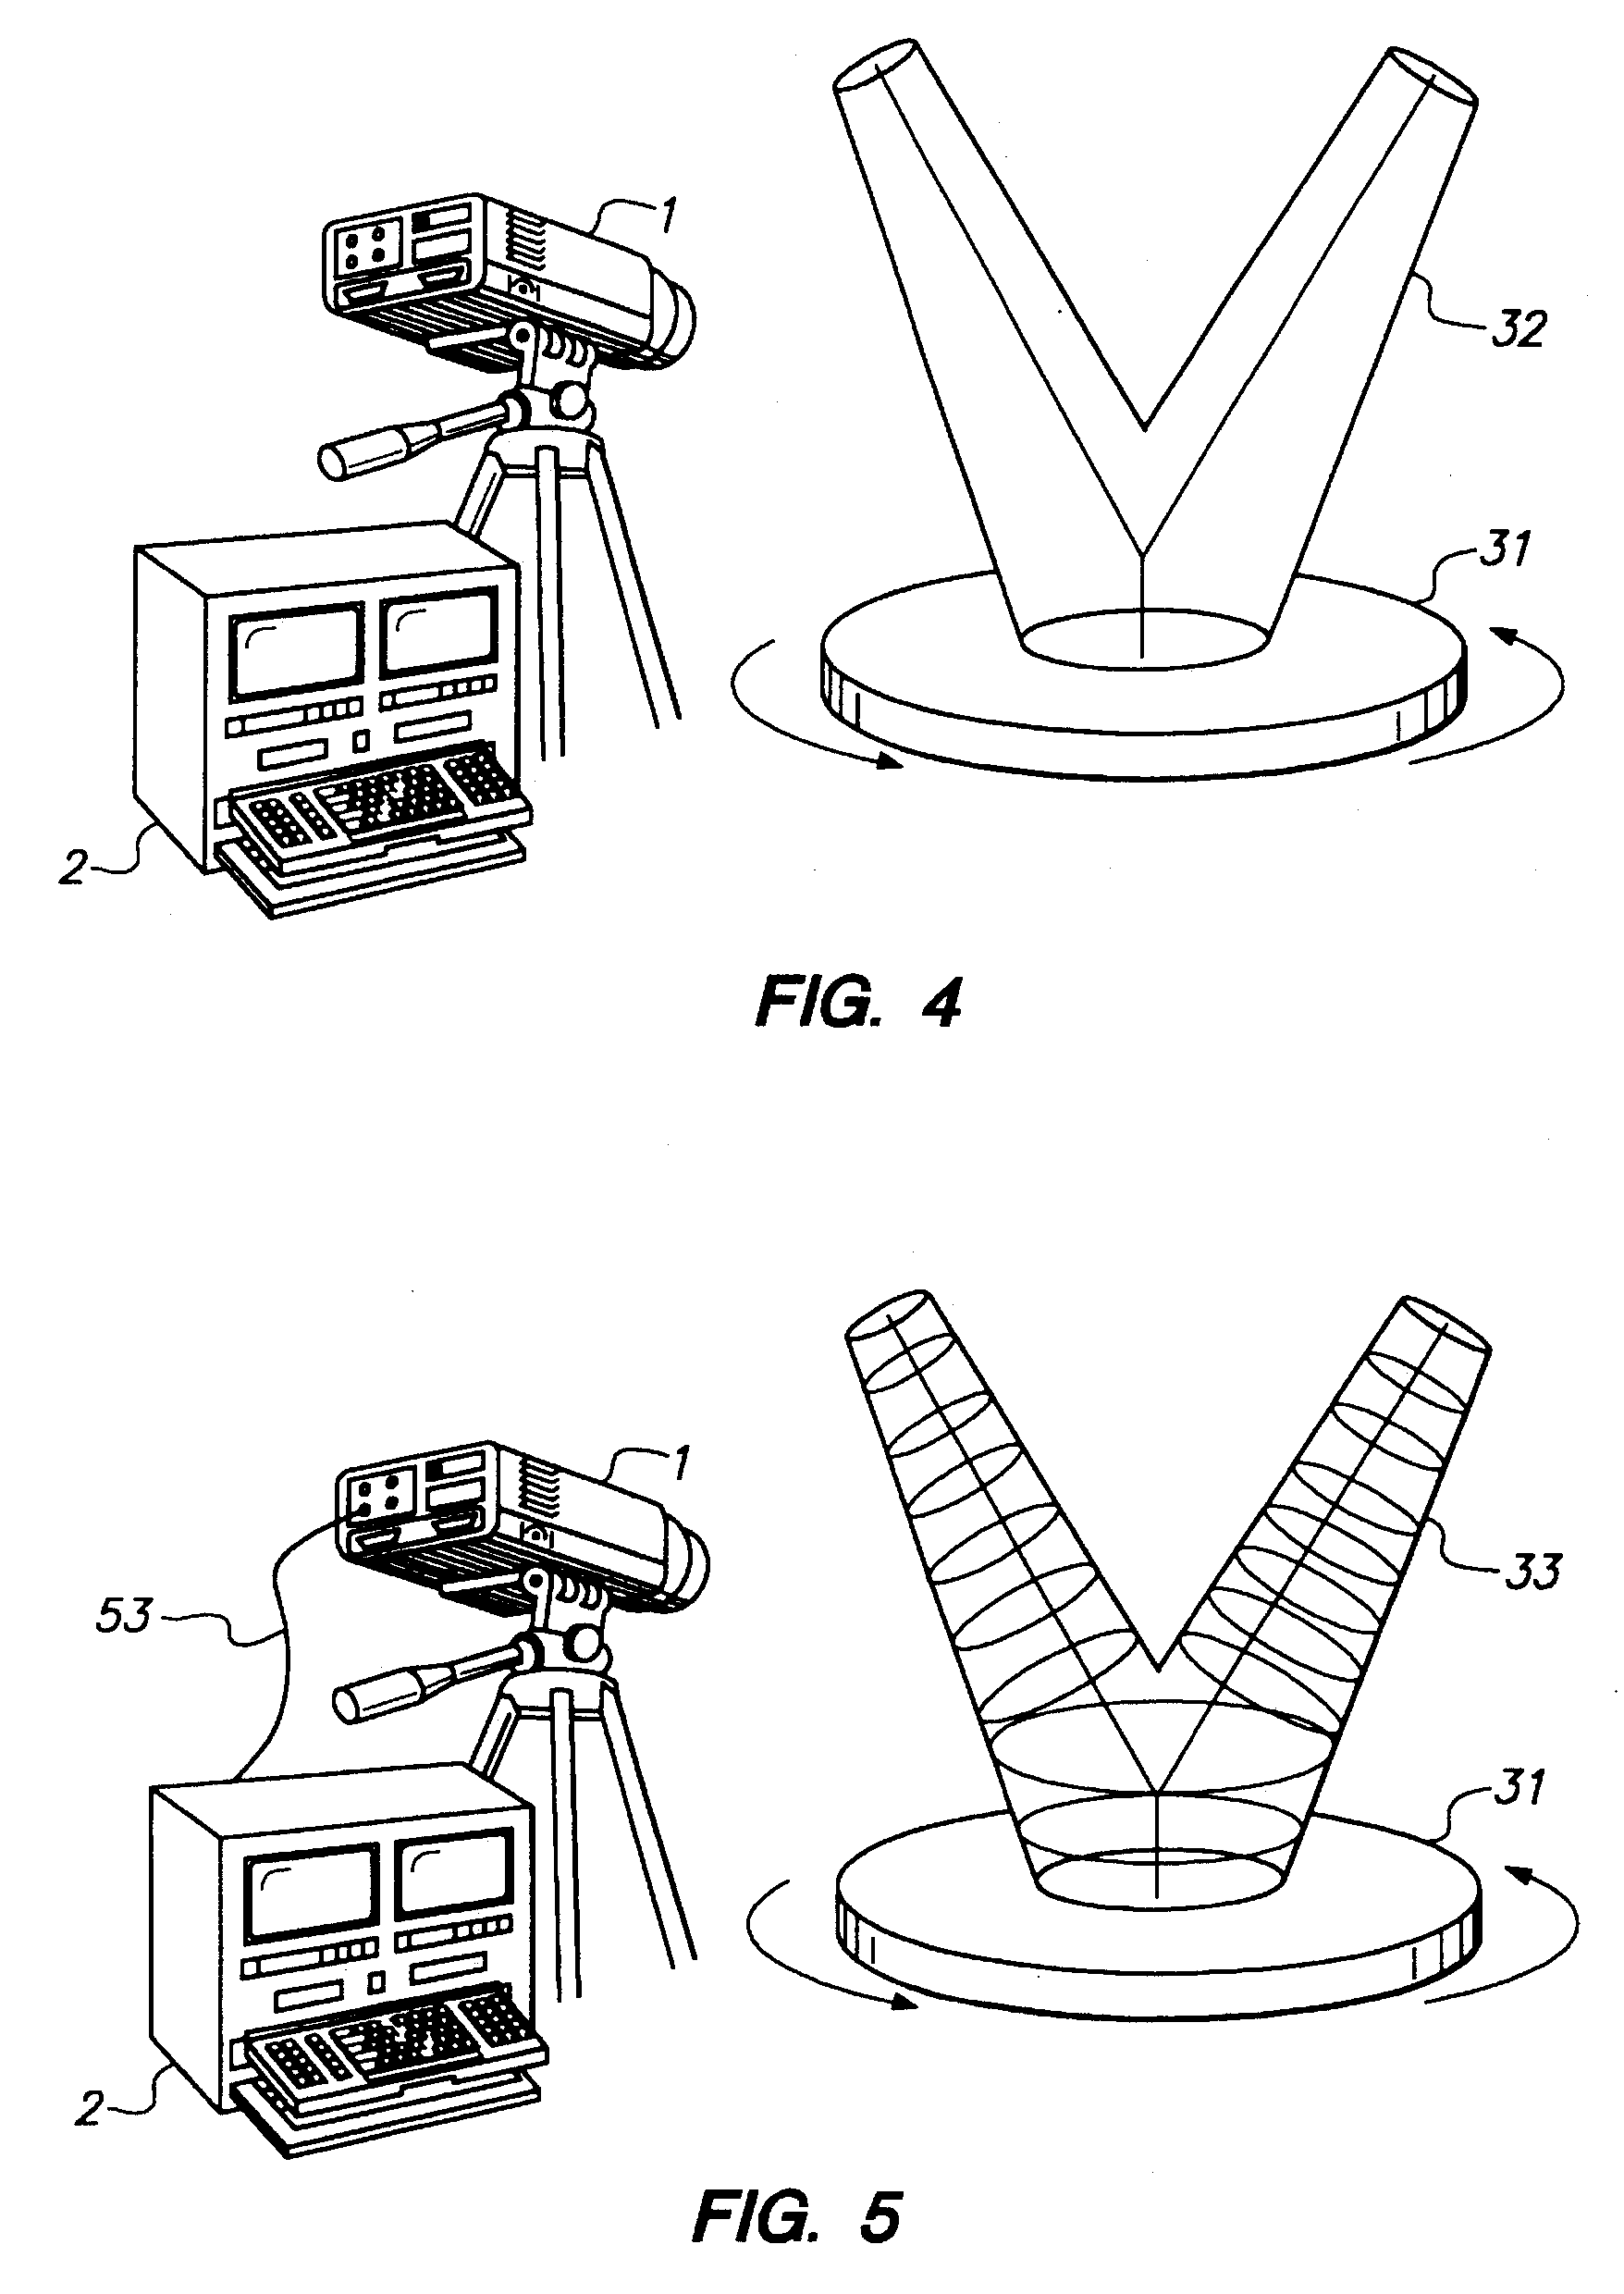
\includegraphics[width=0.3\textwidth]{img/US5530652-drawings-page-7.png}
	\caption[Sistema de captura y digitalización.]{Sistema de captura y digitalización. Fuente \cite{US5530652A}.}
	\label{fig:US5530652-7}
\end{figure}

\begin{figure}[H]
	\centering
	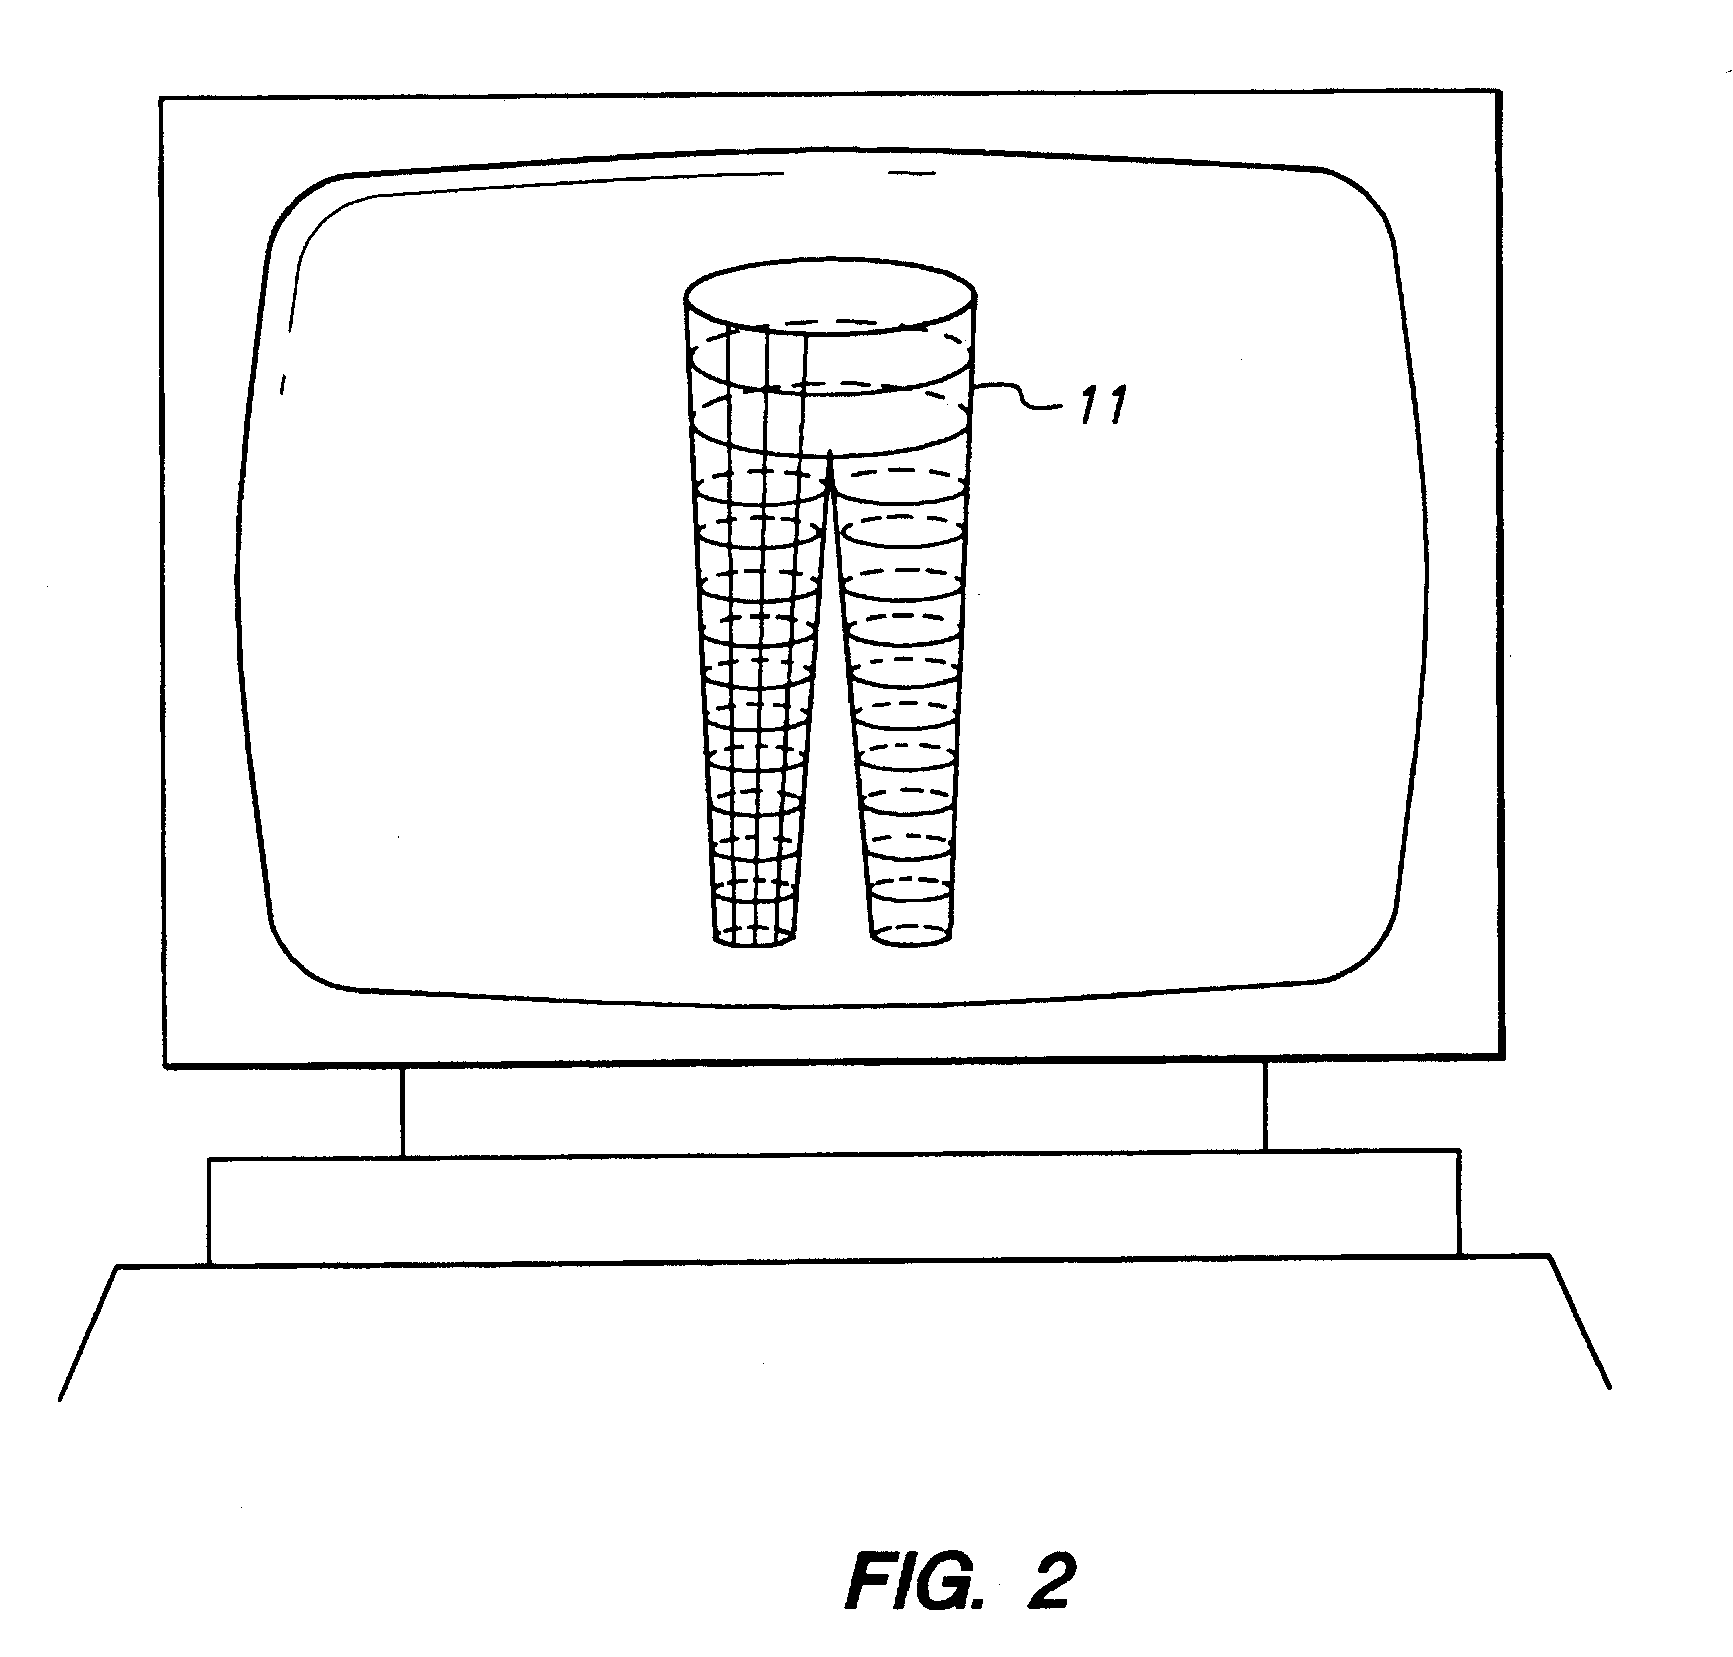
\includegraphics[width=0.4\textwidth]{img/US5530652-drawings-page-5.png}
	\caption[Digitalización de la prenda.]{Digitalización de la prenda. Fuente \cite{US5530652A}.}
	\label{fig:US5530652-5}
\end{figure}

\subsubsection{EP4095520A1}

La patente \cite{EP4095520A1} describe un sistema para el control de calidad de prendas de vestir, diseñado para identificar de manera automática y objetiva defectos tanto visibles como invisibles en la estructura interna de las prendas. Este sistema, como se observa en la Figura \ref{fig:imgf0001} se compone de dos elementos principales: un mecanismo para insuflar un gas de control a una temperatura al menos 20°C superior a la temperatura ambiente en la prenda, y un medio de captura de imágenes para detectar ubicaciones defectuosas en dicha prenda. El gas de control calentado, como aire caliente o vapor, permite detectar defectos gracias a la diferencia de temperatura que se genera en las zonas dañadas o perforadas, sin causar daño adicional a la prenda durante la inspección.

El sistema también puede incluir cámaras térmicas o de luz visible, medios para visualizar el vapor que pasa a través de la prenda y software para generar una imagen 3D de la prenda que facilita la identificación y localización precisa de los defectos. Este enfoque permite un alto grado de automatización y precisión en la detección de defectos, ofreciendo la posibilidad de determinar la naturaleza y severidad de los defectos detectados para posibles reparaciones. Además, el sistema puede ser utilizado para controlar la calidad de prendas de vestir técnicas o de alto rendimiento, asegurando que cumplan con los estándares de calidad requeridos a lo largo de su ciclo de vida, incluso después de múltiples usos y lavados.

\begin{figure}[H]
	\centering
	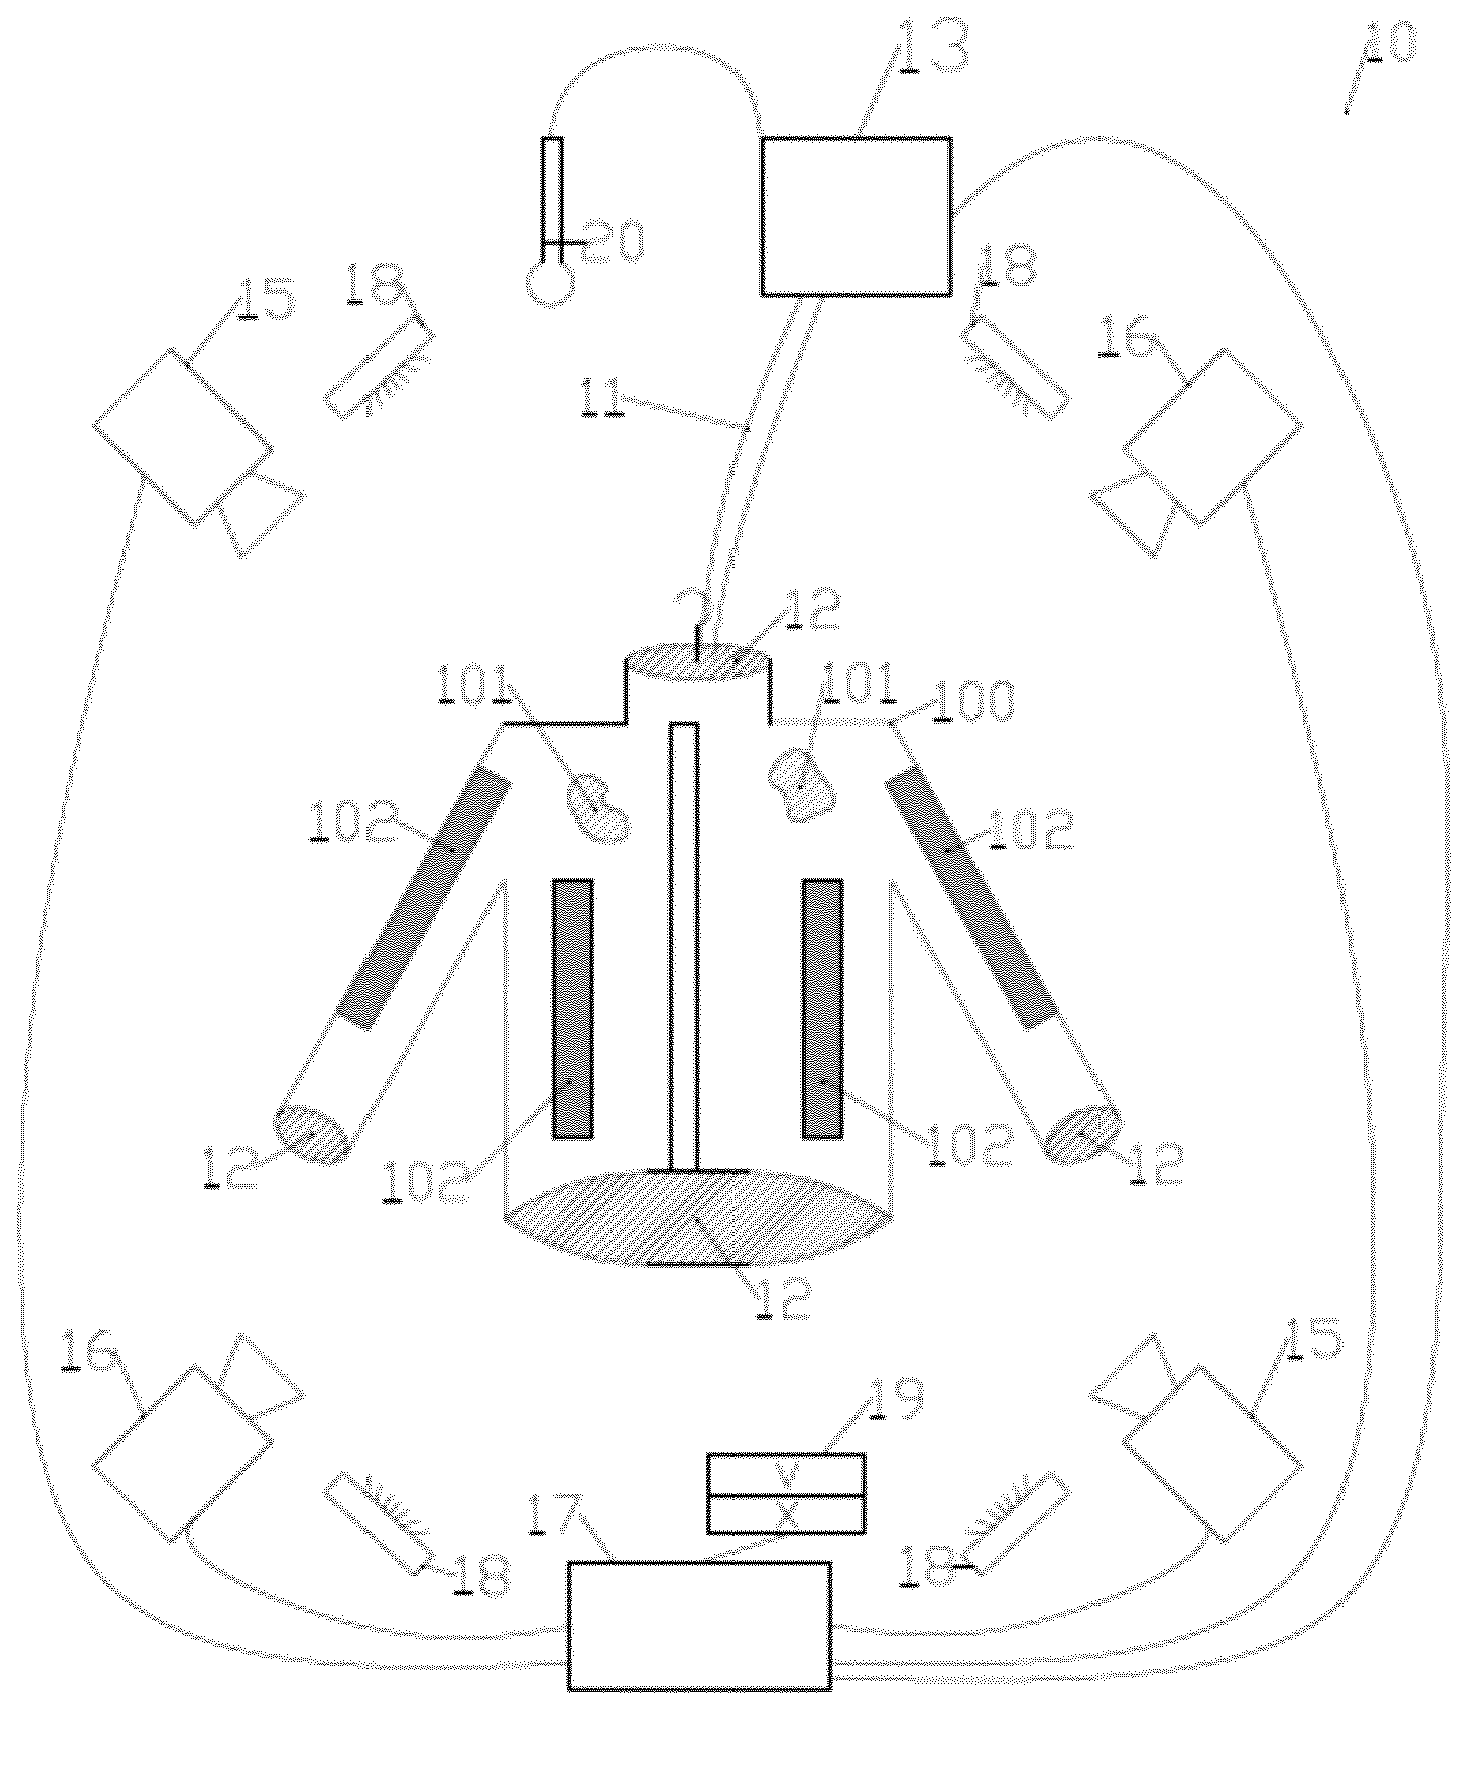
\includegraphics[width=0.4\textwidth]{img/imgf0001.png}
	\caption{Sistema de control de calidad con un mecanismo para insuflar gas.}
	\label{fig:imgf0001}
\end{figure}

\subsubsection{CN218147467U}

La patente \cite{CN218147467U} describe una máquina inteligente de detección de agujas, destinada a abordar problemas específicos en el ámbito de las máquinas de detección de agujas utilizadas para inspeccionar prendas de vestir y otros textiles en busca de partículas metálicas, como agujas rotas. El problema principal que se busca resolver es la limitación en la capacidad de procesamiento de las prendas por las máquinas de detección existentes, que puede llevar a atascos y reducir la eficiencia del proceso de inspección.

La invención se centra en un diseño de máquina de detección de agujas que incluye un escáner montado en la parte superior de un contenedor de la máquina, con mecanismos de ajuste y soporte que permiten desmontar y ajustar el escáner de manera rápida y conveniente. Este diseño permite ajustar el soporte del escáner para manejar diferentes volúmenes de prendas, facilitando la detección de agujas en prendas con variadas capacidades de procesamiento. Los elementos clave del diseño incluyen columnas y placas de soporte ajustables, resortes de soporte, y mecanismos de ajuste de altura que permiten una adaptación flexible a diferentes tamaños y cantidades de prendas.

El diseño inteligente de la máquina de detección de agujas propuesta por esta patente promete mejorar significativamente la eficiencia y flexibilidad de los procesos de inspección de metales en textiles, reduciendo el riesgo de atascos y permitiendo un ajuste rápido y fácil a diferentes necesidades de procesamiento.

\begin{figure}[H]
	\centering
	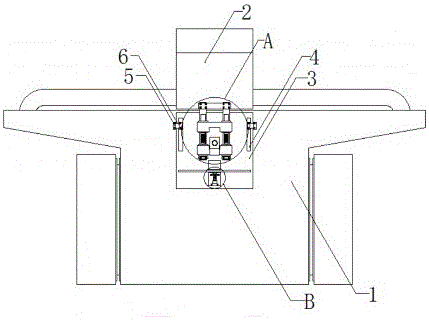
\includegraphics[width=0.6\textwidth]{img/221009135809.png}
	\caption[Detector inteligente de agujas.]{Detector inteligente de agujas. Fuente \cite{CN218147467U}.}
	\label{fig:221009135809}
\end{figure}

% \chapter{Marco Teórico}
% \section{Visión Artificial}
% \subsection{YOLOv8}
% \section{Control de calidad en prendas de vestir}
% \subsection{NTP-ISO 8559-2:2020}

\chapter{Diseño Conceptual}

En este capítulo se presentan alternativas de conceptos solución, los cuales son propuestos en función de la lista de requerimientos, el diagrama de funciones y la matriz morfológica. Luego, los diseños de concepto solución son calificados por una evaluación técnica-económica; con lo cual se obtiene el concepto de solución óptimo.

\section{Lista de exigencias}

Sobre la base de los parámetros necesarios del sistema, los cuales fueron identificados en el Estado del Arte visto en el Capítulo \ref{Estado del Arte}, se elaboró la lista de exigencias mostrada en la Tabla \ref{tab:lista_exigencias}. Esta resume los requerimientos básicos para el diseño del sistema propuesto.

\begin{longtable}{|c|p{4.5em}|p{22.5em}|p{6em}|}
	\caption[Lista de Requerimientos.]{Lista de Requerimientos. Fuente: Elaboración propia.}\label{tab:lista_exigencias}\\
	\hline
	\multicolumn{4}{|p{37.5em}|}{\textbf{LISTA DE EXIGENCIAS}} \bigstrut\\
	\hline
	\multicolumn{2}{|p{9em}|}{\textbf{PROYECTO}} & DISEÑO DE UN SISTEMA PARA EL CONTROL DE CALIDAD DE PRENDAS DE VESTIR UTILIZANDO VISIÓN ARTIFICIAL & Fecha: 06/03/24 \bigstrut\\
	\hline
	\multicolumn{2}{|p{9em}|}{\textbf{CLIENTE}} & Pontificia Universidad Católica del Perú & Elaborado por: A. Luna \bigstrut\\
	\hline
	\multicolumn{2}{|p{9em}|}{\parbox{4cm}{\textbf{FUNCIÓN} \\ \textbf{PRINCIPAL}}
	} & \multicolumn{2}{p{28.5em}|}{Detectar y controlar la calidad de prendas de vestir, identificando tanto los defectos visuales como los relacionados con las medidas.} \bigstrut\\
	\hline
	\endfirsthead \caption* {Tabla \ref{tab:lista_exigencias}: Lista de Requerimientos (Continuación).}\\
	\hline
	\multicolumn{1}{|p{4.5em}|}{\textbf{Fecha}} & \textbf{Deseo o Exigencia} & \textbf{Descripción} & \textbf{Responsable} \bigstrut\\
	\hline
	\endhead
	\multicolumn{4}{|p{37.5em}|}{\textbf{FUNCIONES}} \bigstrut\\
	\hline
	6/03/2024 & E     & La prenda ingresará de manera estirada y sin arrugas. & A. Luna \bigstrut\\
	\hline
	6/03/2024 & E     & Se debe detectar las manchas, hilos salidos y agujeros presentes en las prendas. & A. Luna \bigstrut\\
	\hline
	6/03/2024 & E     & Se debe detectar metales presentes que se hayan dejado en las prendas como agujas o alfileres. & A. Luna \bigstrut\\
	\hline
	\multicolumn{4}{|p{37.5em}|}{\textbf{OPERACIÓN}} \bigstrut\\
	\hline
	6/03/2024 & D     & El prototipo deberá poder controlar la calidad de como mínimo 30 prendas/hora. & A. Luna \bigstrut\\
	\hline
	\multicolumn{4}{|p{37.5em}|}{\textbf{ALIMENTACIÓN}} \bigstrut\\
	\hline
	6/03/2024 & E     & Eléctrica, 220V (Monofásica). & A. Luna \bigstrut\\
	\hline
	\multicolumn{4}{|p{37.5em}|}{\textbf{SOFTWARE}} \bigstrut\\
	\hline
	6/03/2024 & D     & Se debe emplear un software, algoritmo o modelo de código abierto para la implementación de la funcionalidad de la visión por computadora. & A. Luna \bigstrut\\
	\hline
	6/03/2024 & E     & El prototipo debe disponer de una GUI para la interacción con los operarios del sistema.  & A. Luna \bigstrut\\
	\hline
	\multicolumn{4}{|p{37.5em}|}{\textbf{SEÑALES}} \bigstrut\\
	\hline
	6/03/2024 & E     & Entrada: Encendido, apagado, inicio de proceso, fin de proceso.\newline{}Salida: Luz piloto de alimentación, encendido y funcionamiento. & A. Luna \bigstrut\\
	\hline
	\multicolumn{4}{|p{37.5em}|}{\textbf{INTERFAZ}} \bigstrut\\
	\hline
	6/03/2024 & E     & Tablero de control con:\newline{}- Llave de encendido general\newline{}- Pulsador de inicio y parada de proceso\newline{}- Parada de emergencia manual\newline{}- Indicadores luminosos de alimentación,funcionamiento encendido & A. Luna \bigstrut\\
	\hline
	\multicolumn{4}{|p{37.5em}|}{\textbf{CONDICIONES DE OPERACIÓN}} \bigstrut\\
	\hline
	6/03/2024 & E     & Ambiente de trabajo con humedad relativa máxima de 85\%, a 100 msmn (condiciones de la costa peruana, en un laboratorio de pruebas). & A. Luna \bigstrut\\
	\hline
	6/03/2024 & D     & Ambiente de trabajo industrial, con máquinas contiguas trabajando en paralelo. & A. Luna \bigstrut\\
	\hline
	\multicolumn{4}{|p{37.5em}|}{\textbf{CONTROL}} \bigstrut\\
	\hline
	6/03/2024 & E     & Alimentación de ropa manual hecha por un operario. & A. Luna \bigstrut\\
	\hline
	6/03/2024 & E     & Detección de defectos automática. & A. Luna \bigstrut\\
	\hline
	6/03/2024 & E     & Detección de medidas automática. & A. Luna \bigstrut\\
	\hline
	6/03/2024 & D     & Regulación de velocidad de procesamiento de prendas. & A. Luna \bigstrut\\
	\hline
	6/03/2024 & E     & Sensores grado mínimo IP 63 (resistencia al polvo y humedad condensada). & A. Luna \bigstrut\\
	\hline
	6/03/2024 & E     & Parada de emergencia automática en caso de atasco o sobrecarga. & A. Luna \bigstrut\\
	\hline
	\multicolumn{4}{|p{37.5em}|}{\textbf{SEGURIDAD}} \bigstrut\\
	\hline
	6/03/2024 & E     & El tablero de control debe contar con protección contra polvo y liquido grado IP64. & A. Luna \bigstrut\\
	\hline
	\multicolumn{4}{|p{37.5em}|}{\textbf{CONTROL DE CALIDAD}} \bigstrut\\
	\hline
	6/03/2024 & E     & La detección de defectos debe tener una efectividad del 90\%. & A. Luna \bigstrut\\
	\hline
	6/03/2024 & E     & La detección de las medidas de la prenda debe tener una presición del 90\%. & A. Luna \bigstrut\\
	\hline
	\multicolumn{4}{|p{37.5em}|}{\textbf{MONTAJE}} \bigstrut\\
	\hline
	6/03/2024 & D     & El sistema presenta la posibilidad de acoplar varias lineas en paralelo para incrementar la productividad. & A. Luna \bigstrut\\
	\hline
	\multicolumn{4}{|p{37.5em}|}{\textbf{MATERIAL}} \bigstrut\\
	\hline
	6/03/2024 & E     & Materiales que eviten la acumulaciónd de manchas y polvo. & A. Luna \bigstrut\\
	\hline
	\multicolumn{4}{|p{37.5em}|}{\textbf{FABRICACIÓN}} \bigstrut\\
	\hline
	6/03/2024 & E     & El diseño debe contar con componentes estandarizados que esten disponibles en el mercado local. & A. Luna \bigstrut\\
	\hline
	6/03/2024 & D     & Los elementos diseñados deben evitar el mantenimiento complejo. & A. Luna \bigstrut\\
	\hline
	\multicolumn{4}{|p{37.5em}|}{\textbf{MANTENIMIENTO}} \bigstrut\\
	\hline
	6/03/2024 & E     & Los elementos motrices serán accesibles y las superficies fáciles de limpiar. Los componentes electrónicos no deben estar expuestas al polvo. & A. Luna \bigstrut\\
	\hline
	\multicolumn{4}{|p{37.5em}|}{\textbf{DIMENSIONES}} \bigstrut\\
	\hline
	6/03/2024 & E     & El prototipo no deberá ocupar un volumen mayor a 3m x 3m x 3m para poder ser construido en un laboratorio. & A. Luna \bigstrut\\
	\hline
	6/03/2024 & E     & El prototipo no deberá pesar más de 30kg para poder ser movilizado por una persona. & A. Luna \bigstrut\\
	\hline
	\multicolumn{4}{|p{37.5em}|}{\textbf{COSTO}} \bigstrut\\
	\hline
	6/03/2024 & D     & Fabricación: 30000 soles (A nivel de prototipo). & A. Luna \bigstrut\\
	\hline
\end{longtable}%


\section{Estructura de funciones}

La estructura de funciones se utiliza para describir el seguimiento de las señales de entrada y salida dentro del sistema, detallando así la interacción entre las funciones internas de cada dominio. En la subsección \ref{Black Box}, se introducirá el \textit{Black Box}, en el cual se expondrán todas las entradas y salidas pertinentes al sistema. Por otro lado, en la subsección \ref{Funciones Parciales}, se elaborará sobre todas las funciones correspondientes a los subsistemas que integran el sistema en su totalidad, así como las conexiones existentes entre cada una de estas funciones.

\subsection{Black Box}
\label{Black Box}

El diseño de caja negra que se presenta en la Figura \ref{fig:BLACK_BOX} se detallan las entradas y salidas del sistema. La entrada principal del sistema es una prenda de vestir. Para funcionar, este sistema se alimenta de energía a través de una fuente eléctrica estándar de 220VAC monofásica, proporcionando así electricidad a los dominios de transporte, electrónico y de software involucrados. El sistema también está equipado con señales de entrada para su control, incluyendo comandos de inicio, detención y parada de emergencia, tanto en formatos físicos como virtuales. Debido a la ineficiencia de los componentes mecánicos y electrónicos se muestra como salida la energía residual en forma de calor.

\begin{figure}[H]
    \centering
    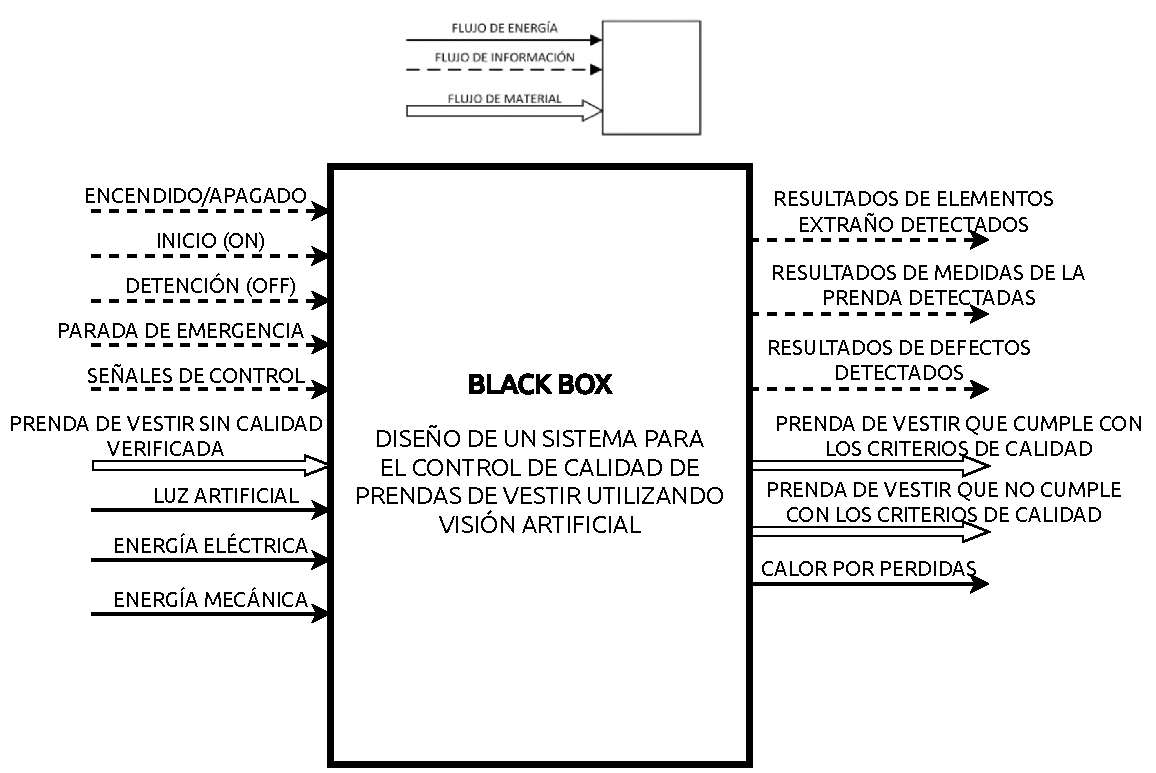
\includegraphics[width=\textwidth]{img/BLACK_BOX.drawio.pdf}
    \caption[Black Box.]{Black Box. Fuente: Elaboración propia.}
    \label{fig:BLACK_BOX}
\end{figure}

\subsection{Funciones Parciales}
\label{Funciones Parciales}

Aquellos procesos que interactúan directamente con el material a ser analizado conforman las funciones básicas del sistema. Estas funciones se muestran en la Figura \ref{fig:ESTRUCTURA_DE_FUNCIONES}. Primero, prendas de vestir sin clasificar son ingresadas por un operario para iniciar el proceso de detección de defectos. Se debe contar además con algún método que maximice la superficie de la prenda que pueda ser visible para la cámara, con el fin de incrementar la efectividad del proceso de detección y clasificación según los criterios de selección. Luego esta prenda es analizada mediante módulos especializados en la detección de defectos visuales y otro módulo encargado de identificar la presencia de elementos metálicos extraños. Como resultado de este proceso, se producirá una imagen que resalta los defectos detectados en la prenda donde se señala la existencia o no de elementos metálicos ajenos. Finalmente, las prendas ya verificadas serán transportadas a la disposición final adecuada.

\begin{sidewaysfigure}
	\begin{figure}[H]
		\centering
		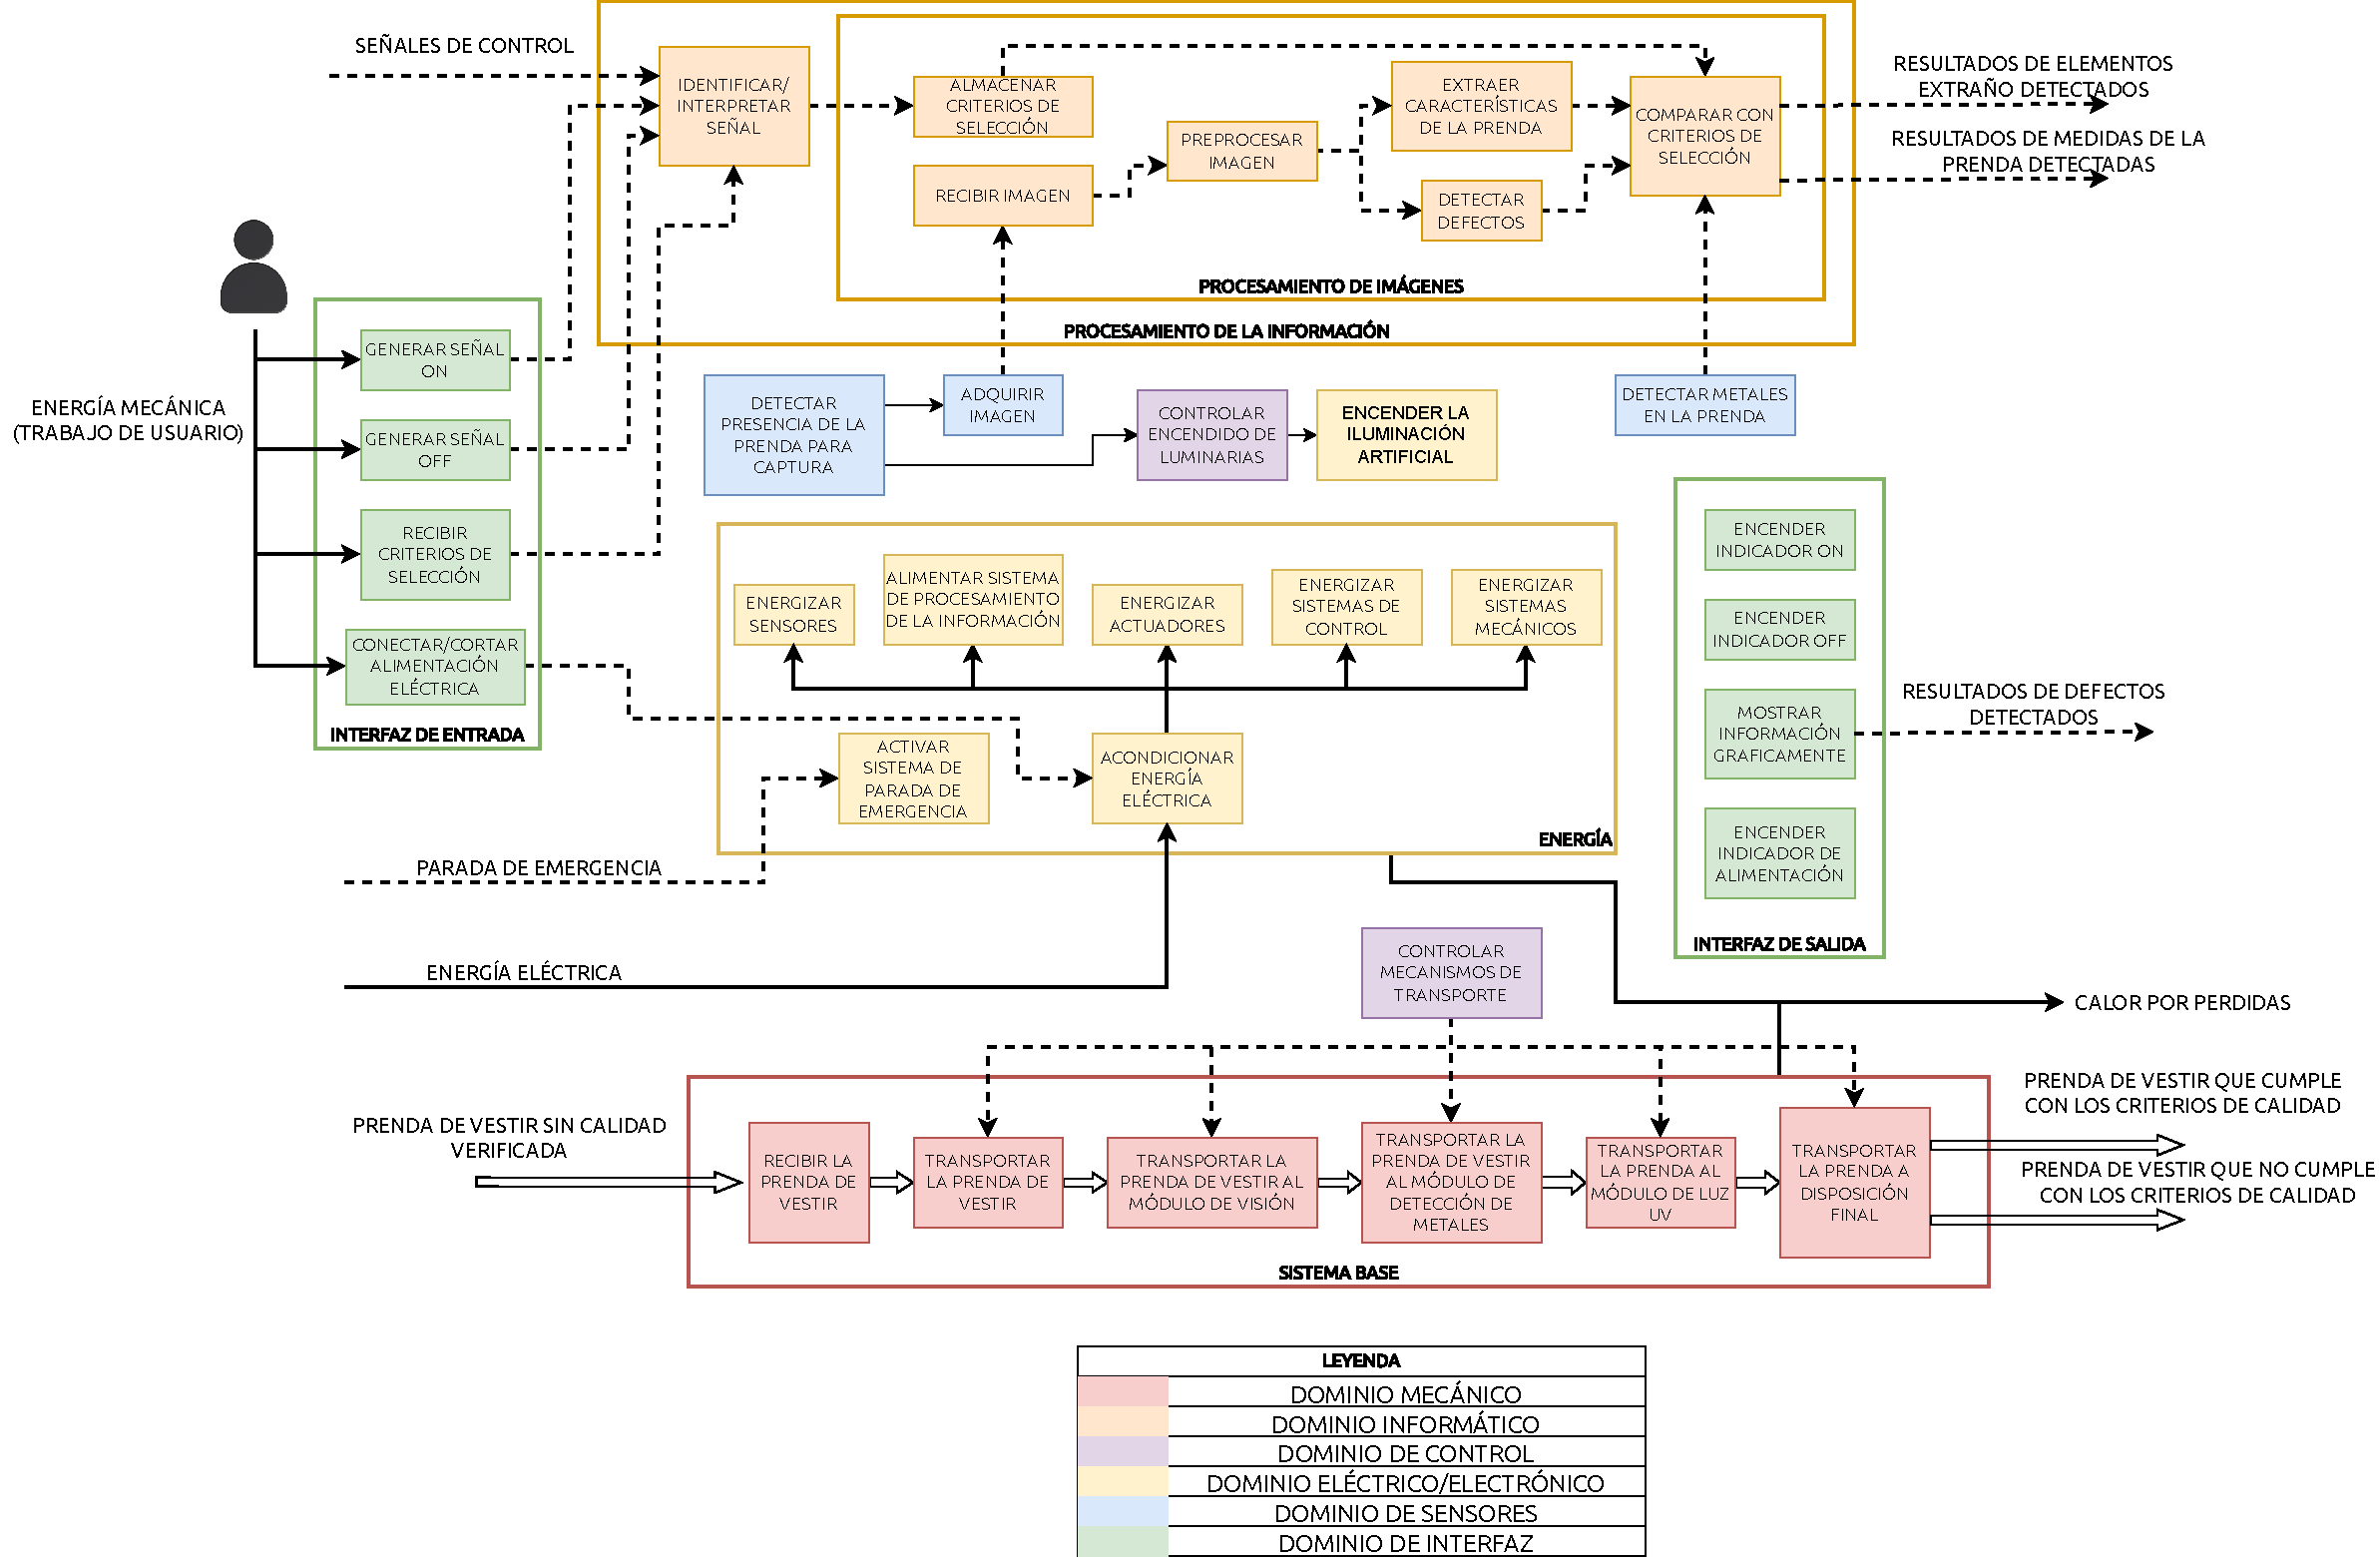
\includegraphics[width=\textwidth]{img/ESTRUCTURA_DE_FUNCIONES.drawio.pdf}
		\label{fig:ESTRUCTURA_DE_FUNCIONES}
		\caption[Estructura de funciones del sistema.]{Estructura de funciones del sistema. Fuente: Elaboración propia.}
	\end{figure}
\end{sidewaysfigure}

\subsubsection{Dominio Mecánico}

El dominio mecánico abarca todas las operaciones físicas y movimientos asociados con el manejo de prendas de vestir, como se muestra en la Figura \ref{fig:EF_DM}. Incluye la recepción de las prendas, su transporte a través de diferentes estaciones de procesamiento como módulos de visión artificial y detección de metales. Este dominio garantiza que las prendas se muevan eficientemente de una etapa a otra, facilitando su análisis y clasificación según cumplan o no con los criterios de calidad establecidos.

\begin{figure}[h]
	\centering
	
\includegraphics[width=\textwidth]{img/EF_DM.pdf}
	\caption[Estructura de funciones del dominio mecánico.]{Estructura de funciones del dominio mecánico. Fuente: Elaboración propia.}
	\label{fig:EF_DM}
\end{figure}

\subsubsection{Dominio Informático}

El dominio informático se centra en el procesamiento de la información obtenida de las prendas , como se muestra en la Figura \ref{fig:EF_DIn}. Este dominio comprende la adquisición y preprocesamiento de imágenes de las prendas, extracción de características relevantes, detección de defectos, y comparación de estos datos con criterios de selección predefinidos para determinar la calidad de las prendas. Este dominio es crucial para interpretar los datos capturados y tomar decisiones basadas en la información procesada.

\begin{figure}[h]
	\centering
	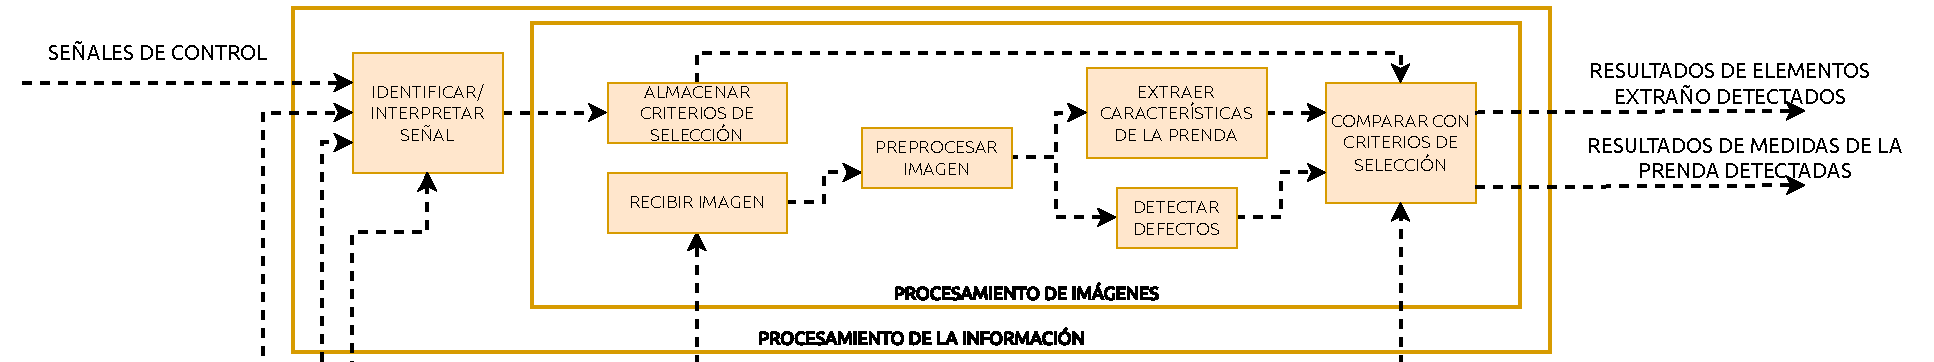
\includegraphics[width=\textwidth]{img/EF_DIn.pdf}
	\caption[Estructura de funciones del dominio informático.]{Estructura de funciones del dominio informático. Fuente: Elaboración propia.}
	\label{fig:EF_DIn}
\end{figure}

\subsubsection{Dominio de Control}

El dominio de control, mostrado en la Figura \ref{fig:EF_DC}, incluye la lógica de control y los mecanismos de decisión que guían las operaciones del sistema. Esto implica generar señales de encendido/apagado basadas en la información procesada, manejar interfaces de entrada/salida, y activar mecanismos de parada de emergencia. Este dominio es esencial para coordinar las actividades de los otros dominios y asegurar que el sistema responda adecuadamente a las condiciones de operación y a los requisitos de procesamiento.

\begin{figure}[h]
	\centering
	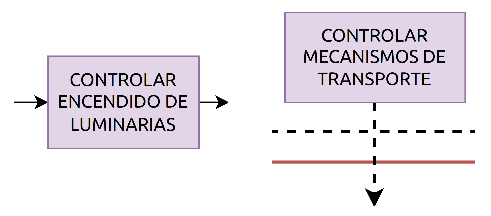
\includegraphics[width=0.4\textwidth]{img/EF_DC.pdf}
	\caption[Estructura de funciones del dominio de control.]{Estructura de funciones del dominio de control. Fuente: Elaboración propia.}
	\label{fig:EF_DC}
\end{figure}

\subsubsection{Dominio Eléctrico/Electrónico}

Este dominio se ocupa de la alimentación y control eléctrico de todos los componentes del sistema, tal y como se muestra en la Figura \ref{fig:EF_DEE}. Desde energizar los sensores hasta alimentar los sistemas de procesamiento de información, actuadores, y sistemas de control, este dominio asegura que todos los elementos electrónicos del sistema reciban la energía necesaria para su funcionamiento. Además, gestiona la iluminación necesaria para la adquisición de imágenes y la señalización a través de indicadores ON/OFF.

\begin{figure}[h]
	\centering
	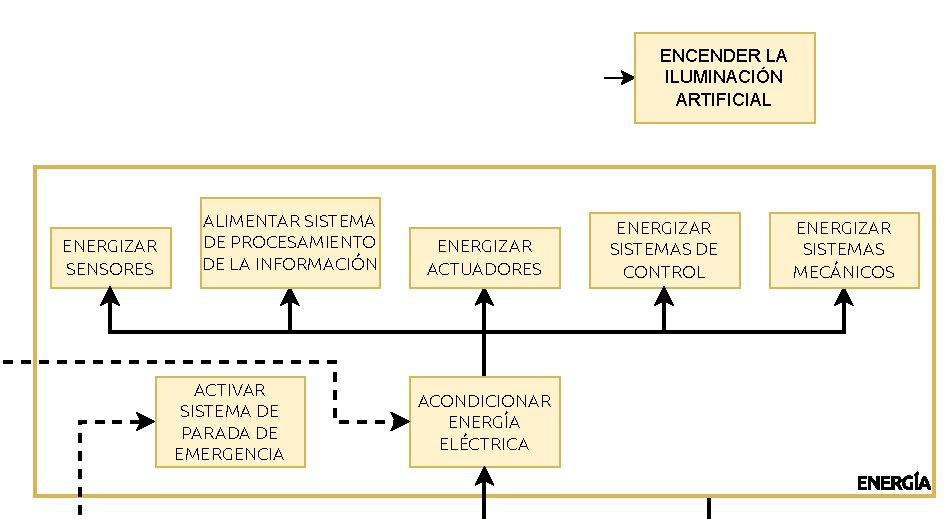
\includegraphics[width=0.8\textwidth]{img/EF_DEE.pdf}
	\caption[Estructura de funciones del dominio eléctrico/electrónico.]{Estructura de funciones del dominio eléctrico/electrónico. Fuente: Elaboración propia.}
	\label{fig:EF_DEE}
\end{figure}

\subsubsection{Dominio de Sensores}

Este dominio comprende la detección y recopilación de datos a través de sensores diseñados para identificar características específicas de las prendas. Esto se muestra en la Figura \ref{fig:EF_DS}. Se identifica la presencia de metales o la preparación para la captura de imágenes. La información recogida por los sensores es vital para el adecuado funcionamiento del sistema, ya que permite adaptar las operaciones a las condiciones actuales y a las necesidades específicas de procesamiento de las prendas.

\begin{figure}[h]
	\centering
	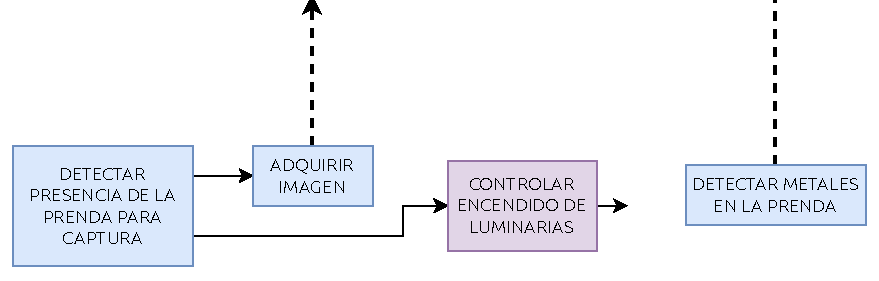
\includegraphics[width=0.7\textwidth]{img/EF_DS.pdf}
	\caption[Estructura de funciones del dominio de sensores.]{Estructura de funciones del dominio de sensores. Fuente: Elaboración propia.}
	\label{fig:EF_DS}
\end{figure}

\subsubsection{Dominio de Interfaz}

El dominio de interfaz esta dedica en interactuar con los usuarios finales del sistema. Como se muestra en la Figura \ref{fig:EF_DI}, a través del empleo de la energía mecánica del operario del sistema para generar las señales de control, lo cual incluye la señal de encendido, apagado o de parada de emergencia. Por otro lado, La información de los resultados de todos los procesos realizados por el sistema se mostraran mediante una interfaz que las muestre de manera ordenada y concisa.

\begin{figure}[h]
	\centering
	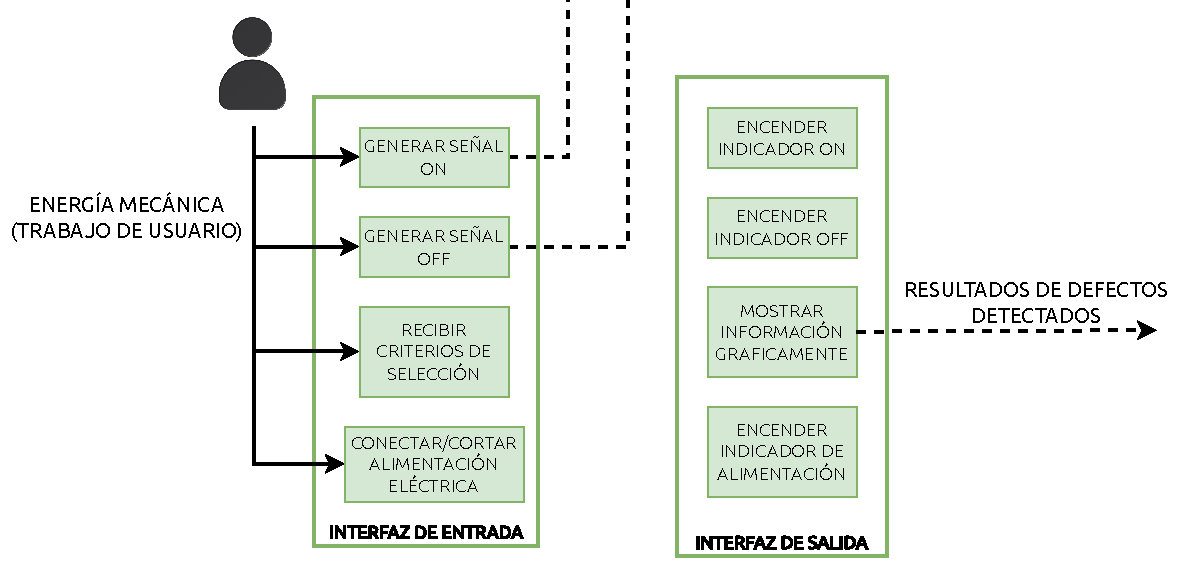
\includegraphics[width=\textwidth]{img/EF_DI.pdf}
	\caption[Estructura de funciones del dominio de interfaz.]{Estructura de funciones del dominio de interfaz. Fuente: Elaboración propia.}
	\label{fig:EF_DI}
\end{figure}

\section{Matriz morfológica}

A continuación, se presentan las diferentes matrices morfológicas para cada dominio previamente descrito, esta metodología ayudó a visualizar las diferentes opciones y escoger una solución idónea para los requerimientos. En las Tablas \ref{tab:MM_DI}, \ref{tab:MM_DM}, \ref{tab:MM_DIn}, \ref{tab:MM_DC}, \ref{tab:MM_DEE} y \ref{tab:MM_DS} se observan las matrices morfológicas del dominio de interfaz, dominio mecánico, dominio informático, dominio de control, dominio eléctrico/electrónico y dominio de sensores respectivamente. 
Las cuatro alternativas de solución se clasificarán siguiendo la leyenda de colores mostrada en la Tabla \ref{tab:leyenda_colores_soluciones}. Estos soluciones se generan al colocar un $\B{\blacklozenge}{1.35}$ con el color correspondiente al concepto de solución para cada función parcial de las matrices morfológicas.

\begin{table}[H]
	\centering
	\caption[Leyenda de colores para los conceptos de solución en las matriz morfológica.]{Leyenda de colores para los conceptos de solución en las matriz morfológica. Fuente: Elaboración propia.}
	\begin{tabular}{|c|c|c|}
		\hline
		\textbf{Soluciones} & \textbf{Tipo de Solución} & \textbf{Color} \bigstrut\\
		\hline
		Solución 1 & Accesible & \cellcolor[rgb]{ 1,  0,  0} \bigstrut\\
		\hline
		Solución 2 & Robusta & \cellcolor[rgb]{ 0,  0,  1} \bigstrut\\
		\hline
		Solución 3 & Precisa & \cellcolor[rgb]{ .298,  .835,  .078} \bigstrut\\
		\hline
	\end{tabular}%
	\label{tab:leyenda_colores_soluciones}%
\end{table}

% ==================== LEYENDA PARA 4 CONCEPTOS DE SOLUCIÓN ====================
%\begin{table}[H]
%	\centering
%	\caption[Leyenda de colores de los conceptos de solución generados en las matrices
%	morfológicas.]{Leyenda de colores de los conceptos de solución generados en las matrices
%		morfológicas. Fuente: Elaboración propia.}
%	\begin{tabular}{|c|c|c|}
%		\hline
%		\textbf{Soluciones} & \textbf{Tipo de Solución} & \textbf{Color} \bigstrut\\
%		\hline
%		Solución 1 & Económica & \cellcolor[rgb]{ 1,  0,  0} \bigstrut\\
%		\hline
%		Solución 2 & Robusta & \cellcolor[rgb]{ 0,  0,  1} \bigstrut\\
%		\hline
%		Solución 3 & Equilibrada & \cellcolor[rgb]{ .298,  .835,  .078} \bigstrut\\
%		\hline
%		Solución 4 & Rápida & \cellcolor[rgb]{ 1,  .502,  0} \bigstrut\\
%		\hline
%	\end{tabular}%
%	\label{tab:leyenda_colores_soluciones}%
%\end{table}


% ==================== PLANTILLA PARA DOMINIO CON 3 SOLUCIONES ====================
%\begin{longtable}{|M{\anchoFPT}|C{6em}|C{6em}|C{6em}|}
%	\caption{Matriz morfológica del dominio de interfaz.}\label{tab:MM_DI}\\
%	\hline
%	\multirow{2}{\anchoFPT}{\parbox{\anchoFPT}{\centering \textbf{FUNCIONES PARCIALES}}} & \multicolumn{3}{c|}{\textbf{DOMINIO INTERFAZ}} \bigstrut\\
%	\cline{2-4} & \textbf{OPCIÓN 1} & \textbf{OPCIÓN 2} & \textbf{OPCIÓN 3} \bigstrut\\
%	\hline
%	\endfirsthead
%	\caption* {Tabla \ref{tab:MM_DI}: Matriz morfológica del dominio de interfaz (Continuación).}\\
%	\hline
%	\multirow{2}{\anchoFPT}{\parbox{\anchoFPT}{\centering \textbf{FUNCIONES PARCIALES}}} & \multicolumn{3}{c|}{\textbf{DOMINIO INTERFAZ}} \bigstrut\\
%	\cline{2-4} & \textbf{OPCIÓN 1} & \textbf{OPCIÓN 2} & \textbf{OPCIÓN 3} \bigstrut\\
%	\hline
%	\endhead
%	\multirow{2}{\anchoFPT}{GENERAR SEÑAL ON Y GENERAR SEÑAL OFF} & \IMM{0.08}{img/botonera1.jpg}{1em} & \IMM{0.1}{img/boton_enc_apa_GUI.jpg}{0.6em} & \IMM{0.12}{img/Switch_tipo_perilla.jpeg}{0.3em} \bigstrut\\
%	\cline{2-4} & Caja con pulsador Start-Stop. \OpR & Botones ON/OFF en GUI. \OpV & Interruptor tipo perilla. \OpA \bigstrut\\
%	\hline
%	\multirow{2}{\anchoFPT}{ENCENDER INDICADOR ON Y ENCENDER INDICADOR OFF} & \IMM{0.13}{img/pilotos_led.jpg}{0.5em} & \IMM{0.14}{img/pantalla_LCD.jpg}{0.3em} & \IMM{0.15}{img/GUI.jpg}{0.1em} \bigstrut\\
%	\cline{2-4} & Pilotos led. \OpA & Pantalla LCD. \OpR & GUI. \OpV \bigstrut\\
%	\hline
%	\multirow{2}{\anchoFPT}{RECIBIR CRITERIOS DE SELECCIÓN} & \IMM{0.13}{img/hmi_industrial.png}{0.2em} & \IMM{0.15}{img/Pantalla_Perilla.jpg}{0.24em} & \IMM{0.15}{img/GUI.jpg}{0.1em} \bigstrut\\
%	\cline{2-4} & HMI Indsutrial. \OpA & Pantalla LCD con perilla de control \OpN & GUI. \OpV \bigstrut\\
%	\hline
%	\multirow{2}{\anchoFPT}{CONECTAR Y CORTAR ALIMENTACIÓN ELÉCTRICA} & \IMM{0.12}{img/termomagnético_diferencial.jpg}{0.7em} & \IMM{0.11}{img/Conmutador_industrial.jpeg}{0.2em} & \IMM{0.11}{img/cable_interruptor.jpg}{0.1em} \bigstrut\\
%	\cline{2-4} & Diferencial con Termomagnético. \OpA \OpV & Conmutador Industrial. \OpN & Cable, enchufe e interruptor. \OpR \bigstrut\\
%	\hline
%	\multirow{2}{\anchoFPT}{MOSTRAR INFORMACIÓN GRAFICAMENTE} & \IMM{0.13}{img/hmi_industrial.png}{0.2em} & \IMM{0.15}{img/GUI.jpg}{0.1em} & \bigstrut\\
%	\cline{2-4} & HMI Indsutrial. \OpR \OpV & GUI.\OpA \OpN &  \bigstrut\\
%	\hline
%\end{longtable}

% =======================================================
%\begin{longtable}{|M{\anchoFPT}|C{6em}|C{6em}|C{6em}|}
%	\caption{Matriz morfológica del dominio de interfaz.}\label{tab:MM_DI}\\
%	\hline
%	\multirow{2}{\anchoFPT}{\parbox{\anchoFPT}{\centering \textbf{FUNCIONES PARCIALES}}} & \multicolumn{3}{c|}{\textbf{DOMINIO }} \bigstrut\\
%	\cline{2-4} & \textbf{OPCIÓN 1} & \textbf{OPCIÓN 2} & \textbf{OPCIÓN 3} \bigstrut\\
%	\hline
%	\endfirsthead
%	\caption* {Tabla \ref{tab:MM_DI}: Matriz morfológica del dominio de interfaz (Continuación).}\\
%	\hline
%	\multirow{2}{\anchoFPT}{\parbox{\anchoFPT}{\centering \textbf{FUNCIONES PARCIALES}}} & \multicolumn{3}{c|}{\textbf{DOMINIO }} \bigstrut\\
%	\cline{2-4} & \textbf{OPCIÓN 1} & \textbf{OPCIÓN 2} & \textbf{OPCIÓN 3} \bigstrut\\
%	\hline
%	\endhead
%	\multirow{2}{\anchoFPT}{} & \IMM{0.08}{img/botonera1.jpg}{1em} & \IMM{0.1}{img/boton_enc_apa_GUI.jpg}{0.6em} & \IMM{0.12}{img/Switch_tipo_perilla.jpeg}{0.3em} \bigstrut\\
%	\cline{2-4} & Caja con pulsador Start-Stop. \OpR & Botones ON/OFF en GUI. \OpV & Interruptor tipo perilla. \OpA \bigstrut\\
%	\hline
%\end{longtable}

\subsection{Dominio de Interfaz}

\begin{longtable}{|M{\anchoFPT}|C{6em}|C{6em}|C{6em}|}
	\caption{Matriz morfológica del dominio de interfaz.}\label{tab:MM_DI}\\
	\hline
	\multirow{2}{\anchoFPT}{\parbox{\anchoFPT}{\centering \textbf{FUNCIONES PARCIALES}}} & \multicolumn{3}{c|}{\textbf{DOMINIO INTERFAZ}} \bigstrut\\
	\cline{2-4} & \textbf{OPCIÓN 1} & \textbf{OPCIÓN 2} & \textbf{OPCIÓN 3} \bigstrut\\
	\hline
	\endfirsthead
	\caption* {Tabla \ref{tab:MM_DI}: Matriz morfológica del dominio de interfaz (Continuación).}\\
	\hline
	\multirow{2}{\anchoFPT}{\parbox{\anchoFPT}{\centering \textbf{FUNCIONES PARCIALES}}} & \multicolumn{3}{c|}{\textbf{DOMINIO INTERFAZ}} \bigstrut\\
	\cline{2-4} & \textbf{OPCIÓN 1} & \textbf{OPCIÓN 2} & \textbf{OPCIÓN 3} \bigstrut\\
	\hline
	\endhead
	\multirow{2}{\anchoFPT}{GENERAR SEÑAL ON Y GENERAR SEÑAL OFF} & \IMM{0.08}{img/botonera1.jpg}{1em} & \IMM{0.1}{img/boton_enc_apa_GUI.jpg}{0.6em} & \IMM{0.12}{img/Switch_tipo_perilla.jpeg}{0.3em} \bigstrut\\
	\cline{2-4} & Caja con pulsador Start-Stop. \OpV & Botones ON/OFF en GUI. \OpR & Interruptor tipo perilla. \OpA \bigstrut\\
	\hline
	\multirow{2}{\anchoFPT}{ENCENDER INDICADOR ON Y ENCENDER INDICADOR OFF} & \IMM{0.13}{img/pilotos_led.jpg}{0.5em} & \IMM{0.14}{img/pantalla_LCD.jpg}{0.3em} & \IMM{0.15}{img/GUI.jpg}{0.1em} \bigstrut\\
	\cline{2-4} & Pilotos led. \OpA & Pantalla LCD. \OpR & GUI. \OpV \bigstrut\\
	\hline
	\multirow{2}{\anchoFPT}{RECIBIR CRITERIOS DE SELECCIÓN} & \IMM{0.13}{img/hmi_industrial.png}{0.2em} & \IMM{0.15}{img/Pantalla_Perilla.jpg}{0.24em} & \IMM{0.15}{img/GUI.jpg}{0.1em} \bigstrut\\
	\cline{2-4} & HMI Indsutrial. \OpA & Pantalla LCD con perilla de control \OpR & GUI. \OpV \bigstrut\\
	\hline
	\multirow{2}{\anchoFPT}{CONECTAR Y CORTAR ALIMENTACIÓN ELÉCTRICA} & \IMM{0.12}{img/termomagnético_diferencial.jpg}{0.7em} & \IMM{0.11}{img/Conmutador_industrial.jpeg}{0.2em} & \IMM{0.11}{img/cable_interruptor.jpg}{0.1em} \bigstrut\\
	\cline{2-4} & Diferencial con Termomagnético. \OpA & Conmutador Industrial. \OpV & Cable, enchufe e interruptor. \OpR \bigstrut\\
	\hline
	\multirow{2}{\anchoFPT}{MOSTRAR INFORMACIÓN GRAFICAMENTE} & \IMM{0.13}{img/hmi_industrial.png}{0.2em} & \IMM{0.15}{img/GUI.jpg}{0.1em} & \bigstrut\\
	\cline{2-4} & HMI Indsutrial. \OpA & GUI.\OpR \OpV &  \bigstrut\\
	\hline
\end{longtable}

%\begin{longtable}{|p{\anchoFP}|C{6em}|C{6em}|C{6em}|C{6em}|}
%	\caption{Matriz morfológica del dominio de interfaz.}\label{tab:MM_DIA}\\
%	\hline
%	\multirow{2}{\anchoFP}{\textbf{FUNCIONES PARCIALES}} & \multicolumn{4}{C{24em}|}{\textbf{DOMINIO DE INTERFAZ}} \bigstrut\\
%	\cline{2-5} & \multicolumn{1}{C{6em}|}{\textbf{OPCIÓN 1}} & \multicolumn{1}{C{6em}|}{\textbf{OPCIÓN 2}} & \multicolumn{1}{C{6em}|}{\textbf{OPCIÓN 3}} & \multicolumn{1}{C{6em}|}{\textbf{OPCIÓN 4}} \bigstrut\\
%	\hline
%	\endfirsthead
%	\caption* {Tabla \ref{tab:MM_DI}: Matriz morfológica del dominio de interfaz (Continuación).}\\
%	\hline
%	\multirow{2}{\anchoFP}{\textbf{FUNCIONES PARCIALES}} & \multicolumn{4}{C{24em}|}{\textbf{DOMINIO DE INTERFAZ}} \bigstrut\\
%	\cline{2-5} & \multicolumn{1}{C{6em}|}{\textbf{OPCIÓN 1}} & \multicolumn{1}{C{6em}|}{\textbf{OPCIÓN 2}} & \multicolumn{1}{C{6em}|}{\textbf{OPCIÓN 3}} & \multicolumn{1}{C{6em}|}{\textbf{OPCIÓN 4}} \bigstrut\\
%	\hline
%	\endhead
%	\multirow{2}{\anchoFP}{GENERAR SEÑAL ON Y GENERAR SEÑAL OFF} & \IMM{0.08}{img/botonera1.jpg}{1em} & \IMM{0.1}{img/boton_enc_apa_GUI.jpg}{0.6em}& \IMM{0.12}{img/Switch_tipo_perilla.jpeg}{0.3em} &\IMM{0.13}{img/Interruptor_tipo_palanca.jpg}{0.3em} \bigstrut\\
%	\cline{2-5} & Caja con pulsador Start-Stop. \OpN & Botones ON/OFF en GUI. \OpV & Interruptor tipo perilla. \OpA & Switch de palanca. \OpR \bigstrut\\
%	\hline	
%	\multirow{2}{\anchoFP}{ENCENDER INDICADOR ON Y ENCENDER INDICADOR OFF} & \IMM{0.12}{img/leds.jpg}{0.7em} & \IMM{0.13}{img/pilotos_led.jpg}{0.5em}& \IMM{0.14}{img/pantalla_LCD.jpg}{0.3em} &\IMM{0.15}{img/GUI.jpg}{0.1em} \bigstrut\\
%	\cline{2-5} & Luces LED. \OpR & Pilotos led. \OpA & Pantalla LCD. \OpN & GUI. \OpV \bigstrut\\
%	\hline
%	\multirow{2}{\anchoFP}{RECIBIR CRITERIOS DE SELECCIÓN} & \IMM{0.13}{img/hmi_industrial.png}{0.2em} & \IMM{0.12}{img/pantalla_tactil.jpg}{0.05em}& \IMM{0.15}{img/Pantalla_Perilla.jpg}{0.24em} & \IMM{0.15}{img/GUI.jpg}{0.1em} \bigstrut\\
%	\cline{2-5} & HMI Indsutrial. \OpA & Pantalla Táctil. \OpR & Pantalla LCD con perilla de control \OpN & GUI. \OpV \bigstrut\\
%	\hline
%	\multirow{2}{\anchoFP}{CONECTAR Y CORTAR ALIMENTACIÓN ELÉCTRICA} & \IMM{0.12}{img/termomagnético_diferencial.jpg}{0.7em} & \IMM{0.11}{img/Conmutador_industrial.jpeg}{0.2em} & \IMM{0.11}{img/cable_interruptor.jpg}{0.1em} & \bigstrut\\
%	\cline{2-5} & Diferencial con Termomagnético. \OpA \OpV & Conmutador Industrial. \OpN & Cable, enchufe e interruptor. \OpR & \bigstrut\\
%	\hline
%	\multirow{2}{\anchoFP}{MOSTRAR INFORMACIÓN GRAFICAMENTE} & \IMM{0.14}{img/hmi_industrial.png}{0.1em} & \IMM{0.15}{img/GUI.jpg}{0.1em} &  &  \bigstrut\\
%	\cline{2-5} & HMI Indsutrial. \OpR \OpV & GUI.\OpA \OpN & & \bigstrut\\
%	\hline
%\end{longtable}

\subsection{Dominio Mecánico}

\begin{longtable}{|M{\anchoFPT}|C{6em}|C{6em}|C{6em}|}
	\caption{Matriz morfológica del dominio mecánico.}\label{tab:MM_DM}\\
	\hline
	\multirow{2}{\anchoFPT}{\parbox{\anchoFPT}{\centering \textbf{FUNCIONES PARCIALES}}} & \multicolumn{3}{c|}{\textbf{DOMINIO MECÁNICO}} \bigstrut\\
	\cline{2-4} & \textbf{OPCIÓN 1} & \textbf{OPCIÓN 2} & \textbf{OPCIÓN 3} \bigstrut\\
	\hline
	\endfirsthead
	\caption* {Tabla \ref{tab:MM_DM}: Matriz morfológica del dominio mecánico (Continuación).}\\
	\hline
	\multirow{2}{\anchoFPT}{\parbox{\anchoFPT}{\centering \textbf{FUNCIONES PARCIALES}}} & \multicolumn{3}{c|}{\textbf{DOMINIO MECÁNICO}} \bigstrut\\
	\cline{2-4} & \textbf{OPCIÓN 1} & \textbf{OPCIÓN 2} & \textbf{OPCIÓN 3} \bigstrut\\
	\hline
	\endhead
	\multirow{2}{\anchoFPT}{TRANSPORTE MECÁNICO DE LAS PRENDAS DE VESTIR} & \IMM{0.14}{img/faja_transportadora_plana.jpg}{0.2em} & \IMM{0.13}{img/faja_transportadora_inclinada.jpg}{0.8em}& \IMM{0.11}{img/conveyer.jpg}{0.2em} \bigstrut\\
	\cline{2-4} & Faja transportadora plana. & Faja transportadora inclinada. & Transportador automático de ropa. \bigstrut\\
	\hline	
	\multirow{2}{\anchoFPT}{GENERAR EL MOVIMIENTO DEL SISTEMA DE TRANSPORTE} & \IMM{0.15}{img/stepper_motor.jpg}{0.3em} & \IMM{0.15}{img/motor_sincrono.jpg}{0.1em}& \IMM{0.14}{img/motor_asincrono.jpg}{0.2em} \bigstrut\\
	\cline{2-4} & Motor a pasos. \OpV & Motor síncrono. \OpA & Motor de inducción. \OpR \bigstrut\\
	\hline
\end{longtable}

%\begin{longtable}{|p{\anchoFP}|C{6em}|C{6em}|C{6em}|C{6em}|}
%	\caption{Matriz morfológica del dominio mecánico.}\label{tab:MM_DM}\\
%	\hline
%	\multirow{2}{\anchoFP}{\textbf{FUNCIONES PARCIALES}} & \multicolumn{4}{C{24em}|}{\textbf{DOMINIO MECÁNICO}} \bigstrut\\
%	\cline{2-5} & \multicolumn{1}{C{6em}|}{\textbf{OPCIÓN 1}} & \multicolumn{1}{C{6em}|}{\textbf{OPCIÓN 2}} & \multicolumn{1}{C{6em}|}{\textbf{OPCIÓN 3}} & \multicolumn{1}{C{6em}|}{\textbf{OPCIÓN 4}} \bigstrut\\
%	\hline
%	\endfirsthead
%	\caption* {Tabla \ref{tab:MM_DM}: Matriz morfológica del dominio mecánico. (Continuación).}\\
%	\hline
%	\multirow{2}{\anchoFP}{\textbf{FUNCIONES PARCIALES}} & \multicolumn{4}{C{24em}|}{\textbf{DOMINIO MECÁNICO}} \bigstrut\\
%	\cline{2-5} & \multicolumn{1}{C{6em}|}{\textbf{OPCIÓN 1}} & \multicolumn{1}{C{6em}|}{\textbf{OPCIÓN 2}} & \multicolumn{1}{C{6em}|}{\textbf{OPCIÓN 3}} & \multicolumn{1}{C{6em}|}{\textbf{OPCIÓN 4}} \bigstrut\\
%	\hline
%	\endhead
%	\multirow{2}{\anchoFP}{TRANSPORTE MECÁNICO DE LAS PRENDAS DE VESTIR} & \IMM{0.14}{img/faja_transportadora_plana.jpg}{0.2em} & \IMM{0.13}{img/faja_transportadora_inclinada.jpg}{0.8em}& \IMM{0.11}{img/conveyer.jpg}{0.2em} &\bigstrut\\
%	\cline{2-5} & Faja transportadora plana. \OpA & Faja transportadora inclinada. \OpR & Transportador automático de ropa. \OpV \OpN& \bigstrut\\
%	\hline	
%	\multirow{2}{\anchoFP}{GENERAR EL MOVIMIENTO DEL SISTEMA DE TRANSPORTE} & \IMM{0.15}{img/stepper_motor.jpg}{0.3em} & \IMM{0.15}{img/motor_sincrono.jpg}{0.1em}& \IMM{0.14}{img/motor_asincrono.jpg}{0.2em} &\IMM{0.14}{img/BLDC.jpg}{0.2em} \bigstrut\\
%	\cline{2-5} & Motor a pasos. \OpA & Motor síncrono. \OpN & Motor de inducción. \OpV & Motor BLDC. \OpR \bigstrut\\
%	\hline
%\end{longtable}

\subsection{Dominio Informático}

\begin{longtable}{|M{\anchoFPT}|C{6em}|C{6em}|C{6em}|}
	\caption{Matriz morfológica del dominio informático.}\label{tab:MM_DIn}\\
	\hline
	\multirow{2}{\anchoFPT}{\parbox{\anchoFPT}{\centering \textbf{FUNCIONES PARCIALES}}} & \multicolumn{3}{c|}{\textbf{DOMINIO INFORMÁTICO}} \bigstrut\\
	\cline{2-4} & \textbf{OPCIÓN 1} & \textbf{OPCIÓN 2} & \textbf{OPCIÓN 3} \bigstrut\\
	\hline
	\endfirsthead
	\caption* {Tabla \ref{tab:MM_DIn}: Matriz morfológica del dominio informático (Continuación).}\\
	\hline
	\multirow{2}{\anchoFPT}{\parbox{\anchoFPT}{\centering \textbf{FUNCIONES PARCIALES}}} & \multicolumn{3}{c|}{\textbf{DOMINIO INFORMÁTICO}} \bigstrut\\
	\cline{2-4} & \textbf{OPCIÓN 1} & \textbf{OPCIÓN 2} & \textbf{OPCIÓN 3} \bigstrut\\
	\hline
	\endhead
	\multirow{2}{\anchoFPT}{IDENTIFICAR E INTERPRETAR LAS SEÑALES} & \IMM{0.13}{img/computadora_industrial.png}{0.5em} & \IMM{0.14}{img/SBC.jpg}{0.3em} & \IMM{0.14}{img/micro.jpg}{0.3em} \bigstrut\\
	\cline{2-4} & Computadora Industrial. \OpA & Single Board Computer (SBC). \OpV & Micro- controlador. \OpR \bigstrut\\
	\hline
	\multirow{2}{\anchoFPT}{ALMACENAR CRITERIOS DE SELECCIÓN} & \IMM{0.11}{img/memoria_sd.jpg}{0.1em} & \IMM{0.12}{img/memoria_tera.jpg}{0.1em} & \IMM{0.12}{img/memoria_ssd.jpg}{0.1em} \bigstrut\\
	\cline{2-4} & Memoria SD. \OpR & Memoria Externa. \OpV & Memoria Interna. \OpA \bigstrut\\
	\hline
	\multirow{2}{\anchoFPT}{PROCESAMIENTO DE IMÁGENES} & \IMM{0.1}{img/opencv.png}{0.5em} & \IMM{0.11}{img/matlab.png}{0.2em} & \IMM{0.12}{img/code.png}{0.2em} \bigstrut\\
	\cline{2-4} & OpenCV (Python) \OpV & MATLAB \OpA & Programación Nativa.\OpR  \bigstrut\\
	\hline
	\multirow{2}{\anchoFPT}{DETECTAR DEFECTOS} & \IMM{0.13}{img/yolov8.jpg}{0.1em} & \IMM{0.13}{img/fasterRCNN.png}{0.1em} & \IMM{0.12}{img/analisis_clasico.png}{0.2em} \bigstrut\\
	\cline{2-4} & YOLOv8. \OpV & Fast R-CNN. \OpA &  Análisis Clásico. \OpR \bigstrut\\
	\hline
\end{longtable}

%\begin{longtable}{|p{\anchoFP}|C{6em}|C{6em}|C{6em}|C{6em}|}
%	\caption{Matriz morfológica del dominio informático.}\label{tab:MM_DIn}\\
%	\hline
%	\multirow{2}{\anchoFP}{\textbf{FUNCIONES PARCIALES}} & \multicolumn{4}{C{24em}|}{\textbf{DOMINIO INFORMÁTICO}} \bigstrut\\
%	\cline{2-5} & \multicolumn{1}{C{6em}|}{\textbf{OPCIÓN 1}} & \multicolumn{1}{C{6em}|}{\textbf{OPCIÓN 2}} & \multicolumn{1}{C{6em}|}{\textbf{OPCIÓN 3}} & \multicolumn{1}{C{6em}|}{\textbf{OPCIÓN 4}} \bigstrut\\
%	\hline
%	\endfirsthead
%	\caption* {Tabla \ref{tab:MM_DIn}: Matriz morfológica del dominio informático (Continuación).}\\
%	\hline
%	\multirow{2}{\anchoFP}{\textbf{FUNCIONES PARCIALES}} & \multicolumn{4}{C{24em}|}{\textbf{DOMINIO INFORMÁTICO}} \bigstrut\\
%	\cline{2-5} & \multicolumn{1}{C{6em}|}{\textbf{OPCIÓN 1}} & \multicolumn{1}{C{6em}|}{\textbf{OPCIÓN 2}} & \multicolumn{1}{C{6em}|}{\textbf{OPCIÓN 3}} & \multicolumn{1}{C{6em}|}{\textbf{OPCIÓN 4}} \bigstrut\\
%	\hline
%	\endhead
%	\multirow{2}{\anchoFP}{IDENTIFICAR E INTERPRETAR LAS SEÑALES} & \IMM{0.13}{img/computadora_industrial.png}{0.5em} & \IMM{0.14}{img/SBC.jpg}{0.3em} & \IMM{0.14}{img/micro.jpg}{0.3em} & \IMM{0.14}{img/FPGA.jpg}{0.2em} \bigstrut\\
%	\cline{2-5} & Computadora Industrial. \OpA & Single Board Computer (SBC). \OpV & Micro- controlador. \OpR & FPGA. \OpN \bigstrut\\
%	\hline
%	\multirow{2}{\anchoFP}{ALMACENAR CRITERIOS DE SELECCIÓN} & \IMM{0.11}{img/memoria_sd.jpg}{0.1em} & \IMM{0.12}{img/memoria_tera.jpg}{0.1em} & \IMM{0.12}{img/memoria_ssd.jpg}{0.1em} & \bigstrut\\
%	\cline{2-5} & Memoria SD. \OpV \OpR & Memoria Externa. \OpN & Memoria Interna. \OpA & \bigstrut\\
%	\hline
%	\multirow{2}{\anchoFP}{PROCESAMIENTO DE IMÁGENES} & \IMM{0.1}{img/opencv.png}{0.5em} & \IMM{0.11}{img/matlab.png}{0.2em} & \IMM{0.12}{img/code.png}{0.2em} & \bigstrut\\
%	\cline{2-5} & OpenCV (Python) \OpV \OpN & MATLAB \OpA & Programación Nativa.\OpR&  \bigstrut\\
%	\hline
%	\multirow{2}{\anchoFP}{DETECTAR DEFECTOS} & \IMM{0.13}{img/yolov8.jpg}{0.1em} & \IMM{0.13}{img/fasterRCNN.png}{0.1em} & \IMM{0.12}{img/analisis_clasico.png}{0.2em} &  \bigstrut\\
%	\cline{2-5} & YOLOv8. \OpV & Fast R-CNN. \OpA &  Análisis Clásico. \OpR \OpN &  \bigstrut\\
%	\hline
%
%\end{longtable}

\subsection{Dominio de Control}

\begin{longtable}{|M{\anchoFPT}|C{6em}|C{6em}|C{6em}|}
	\caption{Matriz morfológica del dominio de control.}\label{tab:MM_DC}\\
	\hline
	\multirow{2}{\anchoFPT}{\parbox{\anchoFPT}{\centering \textbf{FUNCIONES PARCIALES}}} & \multicolumn{3}{c|}{\textbf{DOMINIO DE CONTROL}} \bigstrut\\
	\cline{2-4} & \textbf{OPCIÓN 1} & \textbf{OPCIÓN 2} & \textbf{OPCIÓN 3} \bigstrut\\
	\hline
	\endfirsthead
	\caption* {Tabla \ref{tab:MM_DC}: Matriz morfológica del dominio de control (Continuación).}\\
	\hline
	\multirow{2}{\anchoFPT}{\parbox{\anchoFPT}{\centering \textbf{FUNCIONES PARCIALES}}} & \multicolumn{3}{c|}{\textbf{DOMINIO DE CONTROL}} \bigstrut\\
	\cline{2-4} & \textbf{OPCIÓN 1} & \textbf{OPCIÓN 2} & \textbf{OPCIÓN 3} \bigstrut\\
	\hline
	\endhead
	\multirow{2}{\anchoFPT}{CONTROLAR TRANSPORTES Y LUMINARIA} & \IMM{0.15}{img/ESP32.jpg}{0.08em} & \IMM{0.14}{img/raspberry.jpg}{0.1em} & \IMM{0.14}{img/plc.jpg}{0.1em} \bigstrut\\
	\cline{2-4} & Micro- controlador \OpR & Single Board Computer (SBC). \OpV & PLC. \OpA \bigstrut\\
	\hline
	\multirow{2}{\anchoFPT}{ALGORITMO DE CONTROL} & \IMM{0.16}{img/PID_DISCRETO.png}{0.1em} & \IMM{0.16}{img/onoff_control.png}{0.1em} & \IMM{0.15}{img/realimentacion_estados.png}{0.08em} \bigstrut\\
	\cline{2-4} & PID Discreto. \OpA & Control ON OFF. \OpR & Retro- alimentación de Estados \OpV \bigstrut\\
	\hline
\end{longtable}

%\begin{longtable}{|p{\anchoFP}|C{6em}|C{6em}|C{6em}|C{6em}|}
%	\caption{Matriz morfológica del dominio de control.}\label{tab:MM_DC}\\
%	\hline
%	\multirow{2}{\anchoFP}{\textbf{FUNCIONES PARCIALES}} & \multicolumn{4}{C{24em}|}{\textbf{DOMINIO DE CONTROL}} \bigstrut\\
%	\cline{2-5} & \multicolumn{1}{C{6em}|}{\textbf{OPCIÓN 1}} & \multicolumn{1}{C{6em}|}{\textbf{OPCIÓN 2}} & \multicolumn{1}{C{6em}|}{\textbf{OPCIÓN 3}} & \multicolumn{1}{C{6em}|}{\textbf{OPCIÓN 4}} \bigstrut\\
%	\hline
%	\endfirsthead
%	\caption* {Tabla \ref{tab:MM_DC}: Matriz morfológica del dominio de control (Continuación).}\\
%	\hline
%	\multirow{2}{\anchoFP}{\textbf{FUNCIONES PARCIALES}} & \multicolumn{4}{C{24em}|}{\textbf{DOMINIO DE CONTROL}} \bigstrut\\
%	\cline{2-5} & \multicolumn{1}{C{6em}|}{\textbf{OPCIÓN 1}} & \multicolumn{1}{C{6em}|}{\textbf{OPCIÓN 2}} & \multicolumn{1}{C{6em}|}{\textbf{OPCIÓN 3}} & \multicolumn{1}{C{6em}|}{\textbf{OPCIÓN 4}} \bigstrut\\
%	\hline
%	\endhead
%	\multirow{2}{\anchoFP}{CONTROLAR TRANSPORTES Y LUMINARIA} & \IMM{0.15}{img/ESP32.jpg}{0.08em} & \IMM{0.14}{img/raspberry.jpg}{0.1em} & \IMM{0.14}{img/plc.jpg}{0.1em} & \IMM{0.14}{img/controllogix.jpg}{0.1em} \bigstrut\\
%	\cline{2-5} & Micro- controlador \OpR & Single Board Computer (SBC). \OpV & PLC. \OpN & PAC. \OpA \bigstrut\\
%	\hline
%	\multirow{2}{\anchoFP}{ALGORITMO DE CONTROL} & \IMM{0.16}{img/PID_DISCRETO.png}{0.1em} & \IMM{0.16}{img/control_difuso.jpg}{0.1em} & \IMM{0.16}{img/onoff_control.png}{0.1em} & \IMM{0.15}{img/realimentacion_estados.png}{0.08em} \bigstrut\\
%	\cline{2-5} & PID Discreto. \OpA & Lógica Difusa. \OpN & Control ON OFF. \OpR & Retro- alimentación de Estados \OpV \bigstrut\\
%	\hline
%\end{longtable}

\subsection{Dominio Eléctrico/Electrónico}

\begin{longtable}{|M{\anchoFPT}|C{6em}|C{6em}|C{6em}|}
	\caption{Matriz morfológica del dominio eléctrico/electrónico.}\label{tab:MM_DEE}\\
	\hline
	\multirow{2}{\anchoFPT}{\parbox{\anchoFPT}{\centering \textbf{FUNCIONES PARCIALES}}} & \multicolumn{3}{c|}{\textbf{DOMINIO ELÉCTRICO/ELECTRÓNICO}} \bigstrut\\
	\cline{2-4} & \textbf{OPCIÓN 1} & \textbf{OPCIÓN 2} & \textbf{OPCIÓN 3} \bigstrut\\
	\hline
	\endfirsthead
	\caption* {Tabla \ref{tab:MM_DEE}: Matriz morfológica del dominio eléctrico/electrónico (Continuación).}\\
	\hline
	\multirow{2}{\anchoFPT}{\parbox{\anchoFPT}{\centering \textbf{FUNCIONES PARCIALES}}} & \multicolumn{3}{c|}{\textbf{DOMINIO ELÉCTRICO/ELECTRÓNICO}} \bigstrut\\
	\cline{2-4} & \textbf{OPCIÓN 1} & \textbf{OPCIÓN 2} & \textbf{OPCIÓN 3} \bigstrut\\
	\hline
	\endhead
	\multirow{2}{\anchoFPT}{ACONDICIONAR ENERGÍA ELÉCTRICA} & \IMM{0.13}{img/fuente_switching.jpg}{0.1em} & \IMM{0.13}{img/circuito_rectificador.jpg}{0.1em} & \IMM{0.13}{img/adaptador_AC_DC.jpg}{0.1em} \bigstrut\\
	\cline{2-4} & Fuente Switching. \OpA & Rectificado AC/DC. \OpR & Adaptador AC a DC. \OpV \bigstrut\\
	\hline
	\multirow{2}{\anchoFPT}{ACTIVAR SISTEMA DE PARADA DE EMERGENCIA} & \IMM{0.13}{img/boton_parada_emergencia.jpg}{0.1em} &  &  \bigstrut\\
	\cline{2-4} & Boton de parada de emergencia. \OpR \OpA \OpV  &  &  \bigstrut\\
	\hline
	\multirow{2}{\anchoFPT}{ENERGIZAR SIST. DE CONTROL, SENSORES Y ACTUADORES} & \IMM{0.13}{img/cables_terminal_crimpado.jpg}{0.1em} & \IMM{0.13}{img/cable_motor.jpg}{0.1em} & \bigstrut\\
	\cline{2-4} & Cables con los terminales crimpados. \OpR \OpV & Cables de motor. \OpA & \bigstrut\\
	\hline
	\multirow{2}{\anchoFPT}{ALIMENTAR SISTEMA DE PROCESAMIENTO DE LA INFORMACIÓN} & \IMM{0.11}{img/cable_usb_micro.jpg}{0.1em} & \IMM{0.12}{img/cable_usb_usbB.jpg}{0.1em} & \bigstrut\\
	\cline{2-4} & Cable USB Tipo A a microUSB. \OpR \OpV & Cable USB Tipo A a Tipo B. \OpA & \bigstrut\\
	\hline
\end{longtable}

%\begin{longtable}{|p{\anchoFP}|C{6em}|C{6em}|C{6em}|C{6em}|}
%	\caption{Matriz morfológica del dominio eléctrico/electrónico.}\label{tab:MM_DEE}\\
%	\hline
%	\multirow{2}{\anchoFP}{\textbf{FUNCIONES PARCIALES}} & \multicolumn{4}{C{24em}|}{\textbf{DOMINIO ELÉCTRICO/ELECTRÓNICO}} \bigstrut\\
%	\cline{2-5} & \multicolumn{1}{C{6em}|}{\textbf{OPCIÓN 1}} & \multicolumn{1}{C{6em}|}{\textbf{OPCIÓN 2}} & \multicolumn{1}{C{6em}|}{\textbf{OPCIÓN 3}} & \multicolumn{1}{C{6em}|}{\textbf{OPCIÓN 4}} \bigstrut\\
%	\hline
%	\endfirsthead
%	\caption* {Tabla \ref{tab:MM_DEE}: Matriz morfológica del dominio de interfaz (Continuación).}\\
%	\hline
%	\multirow{2}{\anchoFP}{\textbf{FUNCIONES PARCIALES}} & \multicolumn{4}{C{24em}|}{\textbf{DOMINIO ELÉCTRICO/ELECTRÓNICO}} \bigstrut\\
%	\cline{2-5} & \multicolumn{1}{C{6em}|}{\textbf{OPCIÓN 1}} & \multicolumn{1}{C{6em}|}{\textbf{OPCIÓN 2}} & \multicolumn{1}{C{6em}|}{\textbf{OPCIÓN 3}} & \multicolumn{1}{C{6em}|}{\textbf{OPCIÓN 4}} \bigstrut\\
%	\hline
%	\endhead
%	\multirow{2}{\anchoFP}{ACONDICIONAR ENERGÍA ELÉCTRICA} & \IMM{0.13}{img/fuente_switching.jpg}{0.1em} & \IMM{0.13}{img/circuito_rectificador.jpg}{0.1em} & \IMM{0.13}{img/adaptador_AC_DC.jpg}{0.1em} & \IMM{0.1}{img/rectificador_industrial.jpg}{0.1em} \bigstrut\\
%	\cline{2-5} & Fuente Switching. \OpV & Rectificado AC/DC. \OpR & Adaptador AC a DC. \OpN & Rectificador Industrial. \OpA \bigstrut\\
%	\hline
%	\multirow{2}{\anchoFP}{ACTIVAR SISTEMA DE PARADA DE EMERGENCIA} & \IMM{0.13}{img/boton_parada_emergencia.jpg}{0.1em} &  &  &  \bigstrut\\
%	\cline{2-5} & Boton de parada de emergencia. \OpR \OpA \OpV \OpN &  &  &  \bigstrut\\
%	\hline
%	\multirow{2}{\anchoFP}{ENERGIZAR SIST. DE CONTROL, SENSORES Y ACTUADORES} & \IMM{0.13}{img/cables_terminal_crimpado.jpg}{0.1em} & \IMM{0.13}{img/cable_motor.jpg}{0.1em} &  &  \bigstrut\\
%	\cline{2-5} & Cables con los terminales crimpados. \OpR \OpV & Cables de motor. \OpA \OpN&  &  \bigstrut\\
%	\hline
%	\multirow{2}{\anchoFP}{ALIMENTAR SISTEMA DE PROCESAMIENTO DE LA INFORMACIÓN} & \IMM{0.11}{img/cable_usb_micro.jpg}{0.1em} & \IMM{0.12}{img/cable_usb_usbB.jpg}{0.1em} &  & \bigstrut\\
%	\cline{2-5} & Cable USB Tipo A a microUSB. \OpR \OpV & Cable USB Tipo A a Tipo B. \OpA \OpN &  &  \bigstrut\\
%	\hline
%\end{longtable}

\subsection{Dominio de Sensores}

\begin{longtable}{|M{\anchoFPT}|C{6em}|C{6em}|C{6em}|}
	\caption{Matriz morfológica del dominio de sensores.}\label{tab:MM_DS}\\
	\hline
	\multirow{2}{\anchoFPT}{\parbox{\anchoFPT}{\centering \textbf{FUNCIONES PARCIALES}}} & \multicolumn{3}{c|}{\textbf{DOMINIO DE SENSORES}} \bigstrut\\
	\cline{2-4} & \textbf{OPCIÓN 1} & \textbf{OPCIÓN 2} & \textbf{OPCIÓN 3} \bigstrut\\
	\hline
	\endfirsthead
	\caption* {Tabla \ref{tab:MM_DS}: Matriz morfológica del dominio de sensores. (Continuación).}\\
	\hline
	\multirow{2}{\anchoFPT}{\parbox{\anchoFPT}{\centering \textbf{FUNCIONES PARCIALES}}} & \multicolumn{3}{c|}{\textbf{DOMINIO DE SENSORES}} \bigstrut\\
	\cline{2-4} & \textbf{OPCIÓN 1} & \textbf{OPCIÓN 2} & \textbf{OPCIÓN 3} \bigstrut\\
	\hline
	\endhead
	\multirow{2}{\anchoFPT}{ADQUIRIR IMAGEN} & \IMM{0.13}{img/camara_USB.jpg}{0.1em} & \IMM{0.13}{img/camara_industrial.jpg}{0.1em} & \IMM{0.13}{img/camara_web.jpg}{0.1em} \bigstrut\\
	\cline{2-4} & Cámara USB. \OpV & Cámara Industrial. \OpA & Cámara Web. \OpR \bigstrut\\
	\hline
	\multirow{2}{\anchoFPT}{DETECTAR METALES EN PRENDAS} & \IMM{0.13}{img/detector_agujas.jpg}{0.1em} & \IMM{0.13}{img/detector_metales.png}{0.1em} & \bigstrut\\
	\cline{2-4} & Detector de Agujas. \OpA \OpV & Detector de Metales. \OpR & \bigstrut\\
	\hline
	\multirow{2}{\anchoFPT}{DETECTAR PRESENCIA DE LA PRENDA PARA CAPTURA} & \IMM{0.13}{img/sensor_proximidad_capacitivo.jpg}{0.1em} & \IMM{0.13}{img/sensor_fotoelectrico.jpg}{0.1em} & \IMM{0.13}{img/sensor_ultrasonido.jpg}{0.1em} \bigstrut\\
	\cline{2-4} & Sensor Capacitivo. \OpV & Sensor Fotoeléctrico. \OpA & Sensor Ultrasonido. \OpR \bigstrut\\
	\hline
\end{longtable}

%\begin{longtable}{|p{\anchoFP}|C{6em}|C{6em}|C{6em}|C{6em}|}
%	\caption{Matriz morfológica del dominio de sensores.}\label{tab:MM_DS}\\
%	\hline
%	\multirow{2}{\anchoFP}{\textbf{FUNCIONES PARCIALES}} & \multicolumn{4}{C{24em}|}{\textbf{DOMINIO DE SENSORES}} \bigstrut\\
%	\cline{2-5} & \multicolumn{1}{C{6em}|}{\textbf{OPCIÓN 1}} & \multicolumn{1}{C{6em}|}{\textbf{OPCIÓN 2}} & \multicolumn{1}{C{6em}|}{\textbf{OPCIÓN 3}} & \multicolumn{1}{C{6em}|}{\textbf{OPCIÓN 4}} \bigstrut\\
%	\hline
%	\endfirsthead
%	\caption* {Tabla \ref{tab:MM_DS}: Matriz morfológica del dominio de sensores (Continuación).}\\
%	\hline
%	\multirow{2}{\anchoFP}{\textbf{FUNCIONES PARCIALES}} & \multicolumn{4}{C{24em}|}{\textbf{DOMINIO DE SENSORES}} \bigstrut\\
%	\cline{2-5} & \multicolumn{1}{C{6em}|}{\textbf{OPCIÓN 1}} & \multicolumn{1}{C{6em}|}{\textbf{OPCIÓN 2}} & \multicolumn{1}{C{6em}|}{\textbf{OPCIÓN 3}} & \multicolumn{1}{C{6em}|}{\textbf{OPCIÓN 4}} \bigstrut\\
%	\hline
%	\endhead
%	\multirow{2}{\anchoFP}{ADQUIRIR IMAGEN} & \IMM{0.13}{img/camara_USB.jpg}{0.1em} & \IMM{0.13}{img/camara_industrial.jpg}{0.1em} & \IMM{0.13}{img/camara_web.jpg}{0.1em} & \bigstrut\\
%	\cline{2-5} & Cámara USB. \OpV & Cámara Industrial. \OpA & Cámara Web. \OpN \OpR &  \bigstrut\\
%	\hline
%	\multirow{2}{\anchoFP}{DETECTAR METALES EN PRENDAS} & \IMM{0.13}{img/detector_agujas.jpg}{0.1em} & \IMM{0.13}{img/detector_metales.png}{0.1em} &  &  \bigstrut\\
%	\cline{2-5} & Detector de Agujas. \OpA \OpV & Detector de Metales. \OpR \OpN &  &  \bigstrut\\
%	\hline
%	\multirow{2}{\anchoFP}{DETECTAR PRESENCIA DE LA PRENDA PARA CAPTURA} & \IMM{0.13}{img/sensor_proximidad_capacitivo.jpg}{0.1em} & \IMM{0.13}{img/sensor_fotoelectrico.jpg}{0.1em} & \IMM{0.13}{img/sensor_ultrasonido.jpg}{0.1em} & \IMM{0.13}{img/sensor_laser.jpg}{0.1em} \bigstrut\\
%	\cline{2-5} & Sensor Capacitivo. \OpV & Sensor Fotoeléctrico. \OpN & Sensor Ultrasonido. \OpR & Sensor de Distancia Laser. \OpA \bigstrut\\
%	\hline
%\end{longtable}

\section{Conceptos de solución}

Siguiendo la adaptación de la metodología VDI 2206 \cite{VDIVDE2206_2021}, los conceptos de solución se derivan a partir de las combinaciones de las alternativas propuestas en las matrices morfológicas. Estas soluciones serán objeto de una posterior evaluación con el fin de determinar la solución más óptima para la ejecución del proyecto.

\subsection{Concepto de solución 1}

En el concepto de solución 1, el cual se muestra en la Figura \ref{fig:sketch_CS_1}, se utiliza como sistema de transporte una faja plana, la cual es impulsada por un motor síncrono. Para la unidad de procesamiento, se utiliza un microcontrolador que, a su vez, contiene el sistema de control de todo el sistema. El botón de parada de emergencia, así como el indicador LCD de estado del sistema y la GUI para interactuar con el sistema, se encuentran en un gabinete al costado de la faja transportadora. En la parte inferior de este gabinete, se encuentra el subsistema de acondicionamiento de energía y el cable con switch para hacer la conexión a la toma de corriente. El funcionamiento es que la prenda ingresa al módulo de detección de imágenes mediante el movimiento de la faja; en este módulo, hay una fuente de luz artificial tanto en la parte superior como en la parte inferior del módulo. Posteriormente, la prenda ingresa a un módulo de detección de metales en el que se verifica la presencia de elementos metálicos extraños a la prenda. Una vez finalizada el control de calidad. Mediante la GUI se muestra los resultados de todas las verificaciones.

\begin{figure}[H]
	\centering
	\includegraphics[page=3,width=\textwidth]{img/sketch_CS.pdf}
	\caption[Concepto solución 1.]{Concepto solución 1. Fuente: Elaboración propia.}
	\label{fig:sketch_CS_1}
\end{figure}

\subsection{Concepto de solución 2}

En la segunda propuesta de solución, detallada en la Figura \ref{fig:sketch_CS_2}, se presenta un sistema de transporte tipo \textit{cloth conveyer} que utiliza un riel para el traslado de ropa. El movimiento mecánico se efectúa mediante un motor de pasos para asegurar la precisión en la posición de cada prenda. Incorpora un módulo externo con dos paneles que se aproximan a la prenda al detectar su presencia, presionándola para asegurar su alisado. Estos paneles cuentan con fuentes de luz, sensores ópticos y detectores de metales para inspeccionar la prenda por ambos lados. Además, se incluye un gabinete que alberga la unidad de procesamiento, una SBC encargada del procesamiento de imágenes y del control de movimiento, sensores y actuadores de la máquina. En el mismo gabinete, en su parte inferior, se sitúa el subsistema de acondicionamiento de energía, así como los pilotos LED que indican el estado del sistema y botones de encendido, apagado y parada de emergencia.

\begin{figure}[H]
	\centering
	\includegraphics[page=2,width=\textwidth]{img/sketch_CS.pdf}
	\caption[Concepto solución 2.]{Concepto solución 2. Fuente: Elaboración propia.}
	\label{fig:sketch_CS_2}
\end{figure}

\subsection{Concepto de solución 3}

La representación del concepto de la solución 3 se muestra en la Figura \ref{fig:sketch_CS_3}. Esta solución consiste en un sistema de fajas transportadoras que incluye una faja inclinada con la función de voltear la prenda. Además, el sistema comprende dos módulos, uno al inicio y otro al final, cada uno equipado con un sensor óptico, un detector de metales y una fuente de luz artificial, permitiendo así la inspección de ambos lados de la prenda. La gestión del sistema se lleva a cabo mediante una unidad de procesamiento ubicada en un gabinete, que alberga un PLC y una interfaz hombre-máquina (HMI). En este mismo gabinete se encuentran pilotos LED que muestran el estado del sistema, un interruptor de tipo perilla para el encendido y apagado, y un botón de parada de emergencia.

\begin{figure}[H]
	\centering
	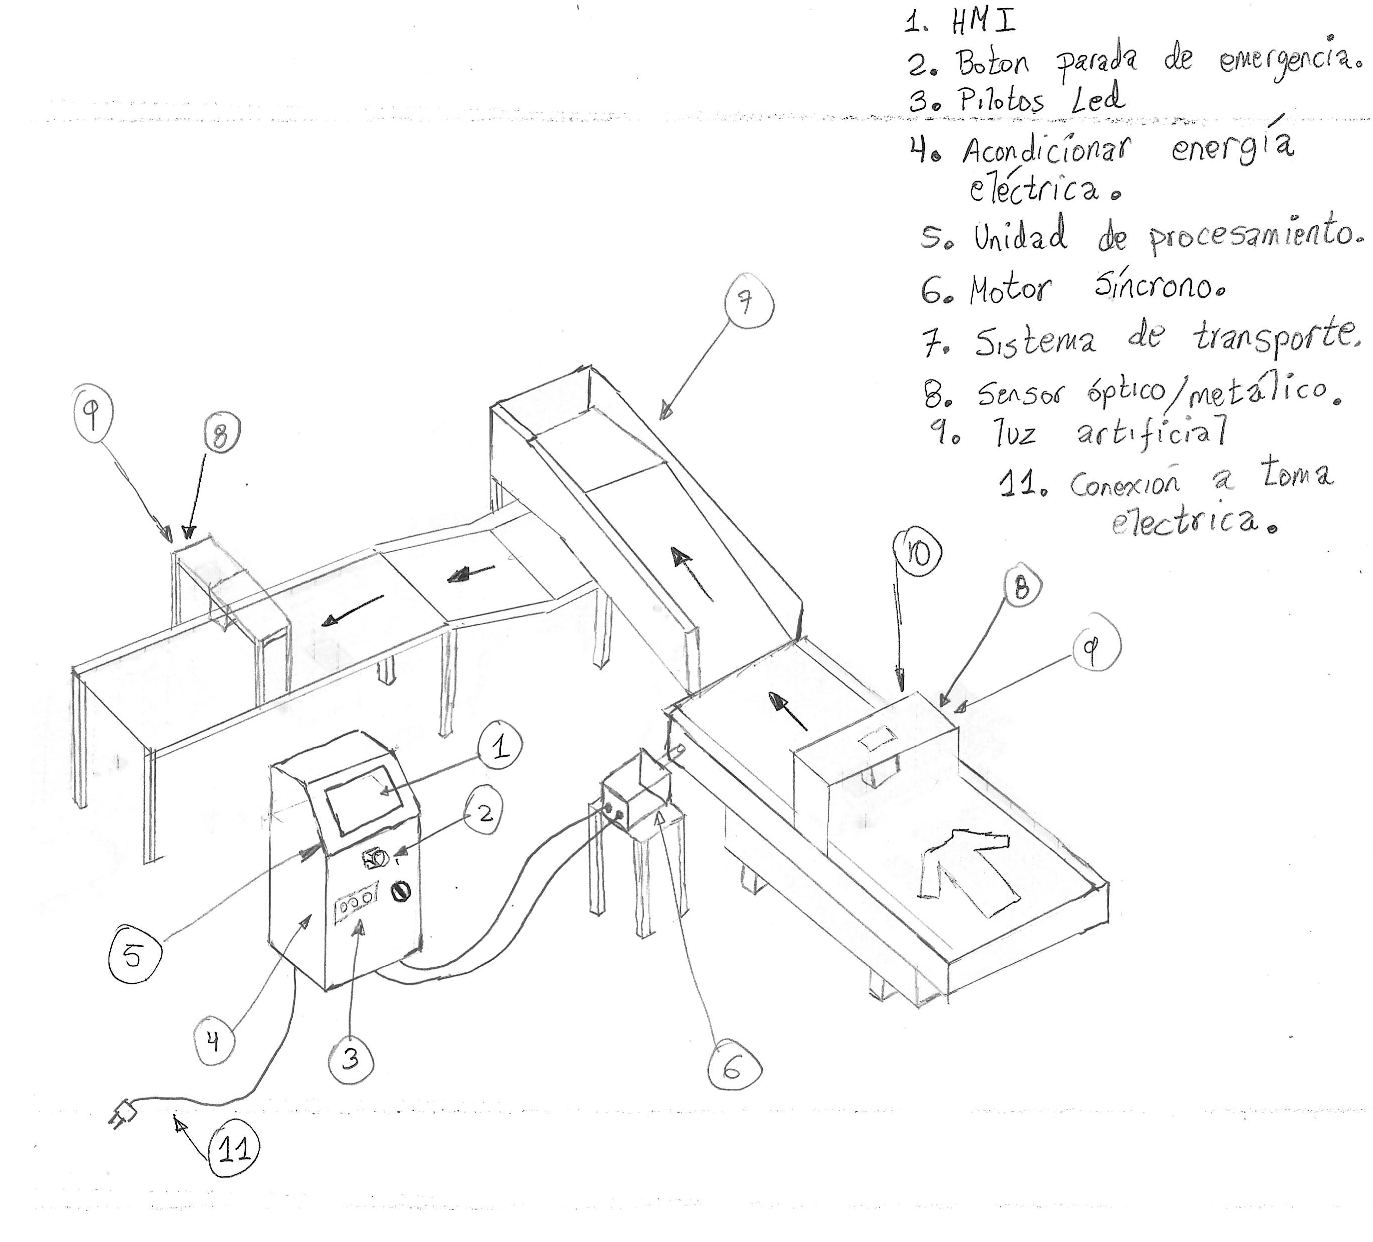
\includegraphics[page=1,width=\textwidth]{img/sketch_CS.pdf}
	\caption[Concepto solución 3.]{Concepto solución 3. Fuente: Elaboración propia.}
	\label{fig:sketch_CS_3}
\end{figure}

\section{Análisis técnico-económica}
% FELIX_RUIZ_JAVIER_DISEÑO_ELECTROGONIÓMETRO_MEDIR

Siguiendo la metodología VDI 2225 \cite{VDI2225_series}, se establecen criterios para evaluar los aspectos técnicos y económicos de las soluciones propuestas. La evaluación técnica y económica se presenta en las Tablas \ref{tab:eval_tecnica} y \ref{tab:eval_economica}, respectivamente. Los criterios tienen pesos diferenciados en el cálculo ponderado, reflejando su importancia en el sistema de acuerdo con la siguiente nomenclatura:

\begin{itemize}
\setlength\itemsep{0em}
	\item El valor de \textbf{g} representa el peso ponderado en función de la importancia del criterio de evaluación.
	\begin{itemize}
	\setlength\itemsep{0em}
		\item 1 = No importante.
		\item 2 = Poco importante.
		\item 3 = Importante.
		\item 4 = Muy importante.
	\end{itemize}
	\item El valor de \textbf{p} representa un puntaje de 0 a 4 (Escala de valores VDI 2225), siendo:
	\begin{itemize}
	\setlength\itemsep{0em}
		\item 0 = No satisface.
		\item 1 = Apenas aceptable.
		\item 2 = Suficiente.
		\item 3 = Bien.
		\item 4 = Excelente (Ideal).
	\end{itemize}
\end{itemize}
	

% Table generated by Excel2LaTeX from sheet 'EVALUACIONES'
\begin{table}[H]
	\centering
	\caption[Evaluación técnica de los conceptos de solución.]{Evaluación técnica de los conceptos de solución. Fuente: Elaboración propia.}
	\begin{tabular}{|c|c|c|c|c|c|c|c|c|c|c|}
		\hline
		\multicolumn{3}{|c|}{\textbf{Evaluación Técnica}} & \multicolumn{2}{c|}{\cellcolor[rgb]{ 1,  0,  0}\textcolor[rgb]{ 1,  1,  1}{\textbf{Solución 1}}} & \multicolumn{2}{c|}{\cellcolor[rgb]{ 0,  0,  1}\textcolor[rgb]{ 1,  1,  1}{\textbf{Solución 2}}} & \multicolumn{2}{c|}{\cellcolor[rgb]{ .298,  .835,  .078}\textbf{Solución 3}} & \multicolumn{2}{c|}{\cellcolor[rgb]{ 1,  .82,  .4}\textbf{Ideal}} \bigstrut\\
		\hline
		\textbf{Nro} & \textbf{Criterio} & \textbf{g} & \textbf{p} & \textbf{p x g} & \textbf{p} & \textbf{p x g} & \textbf{p} & \textbf{p x g} & \textbf{p} & \textbf{p x g} \bigstrut\\
		\hline
		\textbf{1} & \multicolumn{1}{l|}{\textbf{Tamaño}} & \multicolumn{1}{r|}{2} & \multicolumn{1}{r|}{\cellcolor[rgb]{ .949,  .863,  .859}3} & \multicolumn{1}{r|}{6} & \multicolumn{1}{r|}{\cellcolor[rgb]{ .863,  .902,  .945}3} & \multicolumn{1}{r|}{6} & \multicolumn{1}{r|}{\cellcolor[rgb]{ .922,  .945,  .871}2} & \multicolumn{1}{r|}{4} & \multicolumn{1}{r|}{\cellcolor[rgb]{ .992,  .914,  .851}4} & \multicolumn{1}{r|}{8} \bigstrut\\
		\hline
		\textbf{2} & \multicolumn{1}{l|}{\textbf{Dificultad de fabricación}} & \multicolumn{1}{r|}{2} & \multicolumn{1}{r|}{\cellcolor[rgb]{ .949,  .863,  .859}4} & \multicolumn{1}{r|}{8} & \multicolumn{1}{r|}{\cellcolor[rgb]{ .863,  .902,  .945}3} & \multicolumn{1}{r|}{6} & \multicolumn{1}{r|}{\cellcolor[rgb]{ .922,  .945,  .871}2} & \multicolumn{1}{r|}{4} & \multicolumn{1}{r|}{\cellcolor[rgb]{ .992,  .914,  .851}4} & \multicolumn{1}{r|}{8} \bigstrut\\
		\hline
		\textbf{3} & \multicolumn{1}{l|}{\textbf{Calibración}} & \multicolumn{1}{r|}{4} & \multicolumn{1}{r|}{\cellcolor[rgb]{ .949,  .863,  .859}1} & \multicolumn{1}{r|}{4} & \multicolumn{1}{r|}{\cellcolor[rgb]{ .863,  .902,  .945}4} & \multicolumn{1}{r|}{16} & \multicolumn{1}{r|}{\cellcolor[rgb]{ .922,  .945,  .871}2} & \multicolumn{1}{r|}{8} & \multicolumn{1}{r|}{\cellcolor[rgb]{ .992,  .914,  .851}4} & \multicolumn{1}{r|}{16} \bigstrut\\
		\hline
		\textbf{4} & \multicolumn{1}{l|}{\textbf{Tiempo de procesamiento}} & \multicolumn{1}{r|}{4} & \multicolumn{1}{r|}{\cellcolor[rgb]{ .949,  .863,  .859}2} & \multicolumn{1}{r|}{8} & \multicolumn{1}{r|}{\cellcolor[rgb]{ .863,  .902,  .945}4} & \multicolumn{1}{r|}{16} & \multicolumn{1}{r|}{\cellcolor[rgb]{ .922,  .945,  .871}4} & \multicolumn{1}{r|}{16} & \multicolumn{1}{r|}{\cellcolor[rgb]{ .992,  .914,  .851}4} & \multicolumn{1}{r|}{16} \bigstrut\\
		\hline
		\textbf{5} & \multicolumn{1}{l|}{\textbf{Interfaz intuitiva}} & \multicolumn{1}{r|}{3} & \multicolumn{1}{r|}{\cellcolor[rgb]{ .949,  .863,  .859}3} & \multicolumn{1}{r|}{9} & \multicolumn{1}{r|}{\cellcolor[rgb]{ .863,  .902,  .945}4} & \multicolumn{1}{r|}{12} & \multicolumn{1}{r|}{\cellcolor[rgb]{ .922,  .945,  .871}4} & \multicolumn{1}{r|}{12} & \multicolumn{1}{r|}{\cellcolor[rgb]{ .992,  .914,  .851}4} & \multicolumn{1}{r|}{12} \bigstrut\\
		\hline
		\textbf{6} & \multicolumn{1}{l|}{\textbf{Facilidad de manejo }} & \multicolumn{1}{r|}{4} & \multicolumn{1}{r|}{\cellcolor[rgb]{ .949,  .863,  .859}3} & \multicolumn{1}{r|}{12} & \multicolumn{1}{r|}{\cellcolor[rgb]{ .863,  .902,  .945}3} & \multicolumn{1}{r|}{12} & \multicolumn{1}{r|}{\cellcolor[rgb]{ .922,  .945,  .871}3} & \multicolumn{1}{r|}{12} & \multicolumn{1}{r|}{\cellcolor[rgb]{ .992,  .914,  .851}4} & \multicolumn{1}{r|}{16} \bigstrut\\
		\hline
		\textbf{7} & \multicolumn{1}{l|}{\textbf{Seguridad}} & \multicolumn{1}{r|}{4} & \multicolumn{1}{r|}{\cellcolor[rgb]{ .949,  .863,  .859}3} & \multicolumn{1}{r|}{12} & \multicolumn{1}{r|}{\cellcolor[rgb]{ .863,  .902,  .945}3} & \multicolumn{1}{r|}{12} & \multicolumn{1}{r|}{\cellcolor[rgb]{ .922,  .945,  .871}4} & \multicolumn{1}{r|}{16} & \multicolumn{1}{r|}{\cellcolor[rgb]{ .992,  .914,  .851}4} & \multicolumn{1}{r|}{16} \bigstrut\\
		\hline
		\textbf{8} & \multicolumn{1}{l|}{\textbf{Facilidad de mantenimiento}} & \multicolumn{1}{r|}{2} & \multicolumn{1}{r|}{\cellcolor[rgb]{ .949,  .863,  .859}3} & \multicolumn{1}{r|}{6} & \multicolumn{1}{r|}{\cellcolor[rgb]{ .863,  .902,  .945}2} & \multicolumn{1}{r|}{4} & \multicolumn{1}{r|}{\cellcolor[rgb]{ .922,  .945,  .871}3} & \multicolumn{1}{r|}{6} & \multicolumn{1}{r|}{\cellcolor[rgb]{ .992,  .914,  .851}4} & \multicolumn{1}{r|}{8} \bigstrut\\
		\hline
		\textbf{9} & \multicolumn{1}{l|}{\textbf{Durabilidad}} & \multicolumn{1}{r|}{2} & \multicolumn{1}{r|}{\cellcolor[rgb]{ .949,  .863,  .859}2} & \multicolumn{1}{r|}{4} & \multicolumn{1}{r|}{\cellcolor[rgb]{ .863,  .902,  .945}2} & \multicolumn{1}{r|}{4} & \multicolumn{1}{r|}{\cellcolor[rgb]{ .922,  .945,  .871}3} & \multicolumn{1}{r|}{6} & \multicolumn{1}{r|}{\cellcolor[rgb]{ .992,  .914,  .851}4} & \multicolumn{1}{r|}{8} \bigstrut\\
		\hline
		\rowcolor[rgb]{ .851,  .851,  .851} \multicolumn{3}{|c|}{\textbf{Suma}} & \multicolumn{1}{r|}{24} & \multicolumn{1}{r|}{69} & \multicolumn{1}{r|}{28} & \multicolumn{1}{r|}{88} & \multicolumn{1}{r|}{27} & \multicolumn{1}{r|}{84} & \multicolumn{1}{r|}{36} & \multicolumn{1}{r|}{108} \bigstrut\\
		\hline
		\multicolumn{3}{|c|}{\textbf{Promedio}} & \multicolumn{1}{r|}{0.667} & \multicolumn{1}{r|}{\cellcolor[rgb]{ 1,  1,  0}0.639} & \multicolumn{1}{r|}{0.778} & \multicolumn{1}{r|}{\cellcolor[rgb]{ 1,  1,  0}0.815} & \multicolumn{1}{r|}{0.750} & \multicolumn{1}{r|}{\cellcolor[rgb]{ 1,  1,  0}0.778} & \multicolumn{1}{r|}{1} & \multicolumn{1}{r|}{\cellcolor[rgb]{ 1,  1,  0}1} \bigstrut\\
		\hline
		\multicolumn{3}{|c|}{\textbf{Orden}} & \multicolumn{2}{c|}{3} & \multicolumn{2}{c|}{1} & \multicolumn{2}{c|}{2} & \multicolumn{2}{c|}{} \bigstrut\\
		\hline
	\end{tabular}%
	\label{tab:eval_tecnica}%
\end{table}%

% Table generated by Excel2LaTeX from sheet 'EVALUACIONES'
\begin{table}[H]
	\centering
	\caption[Evaluación económica de los conceptos de solución.]{Evaluación económica de los conceptos de solución. Fuente: Elaboración propia.}
	\begin{tabular}{|c|c|c|c|c|c|c|c|c|c|c|}
		\hline
		\multicolumn{3}{|c|}{\textbf{Evaluación Técnica}} & \multicolumn{2}{c|}{\cellcolor[rgb]{ 1,  0,  0}\textcolor[rgb]{ 1,  1,  1}{\textbf{Solución 1}}} & \multicolumn{2}{c|}{\cellcolor[rgb]{ 0,  0,  1}\textcolor[rgb]{ 1,  1,  1}{\textbf{Solución 2}}} & \multicolumn{2}{c|}{\cellcolor[rgb]{ .298,  .835,  .078}\textbf{Solución 3}} & \multicolumn{2}{c|}{\cellcolor[rgb]{ 1,  .82,  .4}\textbf{Ideal}} \bigstrut\\
		\hline
		\textbf{Nro} & \textbf{Criterio} & \textbf{g} & \textbf{p} & \textbf{p x g} & \textbf{p} & \textbf{p x g} & \textbf{p} & \textbf{p x g} & \textbf{p} & \textbf{p x g} \bigstrut\\
		\hline
		\textbf{1} & \multicolumn{1}{l|}{\textbf{Número de piezas}} & \multicolumn{1}{r|}{2} & \multicolumn{1}{r|}{\cellcolor[rgb]{ .949,  .863,  .859}3} & \multicolumn{1}{r|}{6} & \multicolumn{1}{r|}{\cellcolor[rgb]{ .863,  .902,  .945}3} & \multicolumn{1}{r|}{6} & \multicolumn{1}{r|}{\cellcolor[rgb]{ .922,  .945,  .871}3} & \multicolumn{1}{r|}{6} & \multicolumn{1}{r|}{\cellcolor[rgb]{ .992,  .914,  .851}4} & \multicolumn{1}{r|}{8} \bigstrut\\
		\hline
		\textbf{2} & \multicolumn{1}{l|}{\textbf{Costo de componentes}} & \multicolumn{1}{r|}{3} & \multicolumn{1}{r|}{\cellcolor[rgb]{ .949,  .863,  .859}3} & \multicolumn{1}{r|}{9} & \multicolumn{1}{r|}{\cellcolor[rgb]{ .863,  .902,  .945}3} & \multicolumn{1}{r|}{9} & \multicolumn{1}{r|}{\cellcolor[rgb]{ .922,  .945,  .871}2} & \multicolumn{1}{r|}{6} & \multicolumn{1}{r|}{\cellcolor[rgb]{ .992,  .914,  .851}4} & \multicolumn{1}{r|}{12} \bigstrut\\
		\hline
		\textbf{3} & \multicolumn{1}{l|}{\textbf{Disponibilidad de materiales}} & \multicolumn{1}{r|}{4} & \multicolumn{1}{r|}{\cellcolor[rgb]{ .949,  .863,  .859}3} & \multicolumn{1}{r|}{12} & \multicolumn{1}{r|}{\cellcolor[rgb]{ .863,  .902,  .945}2} & \multicolumn{1}{r|}{8} & \multicolumn{1}{r|}{\cellcolor[rgb]{ .922,  .945,  .871}1} & \multicolumn{1}{r|}{4} & \multicolumn{1}{r|}{\cellcolor[rgb]{ .992,  .914,  .851}4} & \multicolumn{1}{r|}{16} \bigstrut\\
		\hline
		\textbf{4} & \multicolumn{1}{l|}{\textbf{Costo de Tecnología}} & \multicolumn{1}{r|}{4} & \multicolumn{1}{r|}{\cellcolor[rgb]{ .949,  .863,  .859}2} & \multicolumn{1}{r|}{8} & \multicolumn{1}{r|}{\cellcolor[rgb]{ .863,  .902,  .945}3} & \multicolumn{1}{r|}{12} & \multicolumn{1}{r|}{\cellcolor[rgb]{ .922,  .945,  .871}2} & \multicolumn{1}{r|}{8} & \multicolumn{1}{r|}{\cellcolor[rgb]{ .992,  .914,  .851}2} & \multicolumn{1}{r|}{8} \bigstrut\\
		\hline
		\textbf{5} & \multicolumn{1}{l|}{\textbf{Costo de Fabricación}} & \multicolumn{1}{r|}{4} & \multicolumn{1}{r|}{\cellcolor[rgb]{ .949,  .863,  .859}3} & \multicolumn{1}{r|}{12} & \multicolumn{1}{r|}{\cellcolor[rgb]{ .863,  .902,  .945}4} & \multicolumn{1}{r|}{16} & \multicolumn{1}{r|}{\cellcolor[rgb]{ .922,  .945,  .871}2} & \multicolumn{1}{r|}{8} & \multicolumn{1}{r|}{\cellcolor[rgb]{ .992,  .914,  .851}4} & \multicolumn{1}{r|}{16} \bigstrut\\
		\hline
		\textbf{6} & \multicolumn{1}{l|}{\textbf{Costo de Mantenimiento}} & \multicolumn{1}{r|}{2} & \multicolumn{1}{r|}{\cellcolor[rgb]{ .949,  .863,  .859}2} & \multicolumn{1}{r|}{4} & \multicolumn{1}{r|}{\cellcolor[rgb]{ .863,  .902,  .945}2} & \multicolumn{1}{r|}{4} & \multicolumn{1}{r|}{\cellcolor[rgb]{ .922,  .945,  .871}2} & \multicolumn{1}{r|}{4} & \multicolumn{1}{r|}{\cellcolor[rgb]{ .992,  .914,  .851}4} & \multicolumn{1}{r|}{8} \bigstrut\\
		\hline
		\rowcolor[rgb]{ .851,  .851,  .851} \multicolumn{3}{|c|}{\textbf{Suma}} & \multicolumn{1}{r|}{16} & \multicolumn{1}{r|}{51} & \multicolumn{1}{r|}{17} & \multicolumn{1}{r|}{55} & \multicolumn{1}{r|}{12} & \multicolumn{1}{r|}{36} & \multicolumn{1}{r|}{22} & \multicolumn{1}{r|}{68} \bigstrut\\
		\hline
		\multicolumn{3}{|c|}{\textbf{Promedio}} & \multicolumn{1}{r|}{0.727} & \multicolumn{1}{r|}{\cellcolor[rgb]{ 1,  1,  0}0.750} & \multicolumn{1}{r|}{0.773} & \multicolumn{1}{r|}{\cellcolor[rgb]{ 1,  1,  0}0.809} & \multicolumn{1}{r|}{0.545} & \multicolumn{1}{r|}{\cellcolor[rgb]{ 1,  1,  0}0.529} & \multicolumn{1}{r|}{1} & \multicolumn{1}{r|}{\cellcolor[rgb]{ 1,  1,  0}1} \bigstrut\\
		\hline
		\multicolumn{3}{|c|}{\textbf{Orden}} & \multicolumn{2}{c|}{2} & \multicolumn{2}{c|}{1} & \multicolumn{2}{c|}{3} & \multicolumn{2}{c|}{} \bigstrut\\
		\hline
	\end{tabular}%
	\label{tab:eval_economica}%
\end{table}%


Basándonos en los datos de las Tablas \ref{tab:eval_tecnica} y \ref{tab:eval_economica}, realizamos un estudio técnico y económico que nos permite identificar la mejor solución. La Figura \ref{fig:comp_tecnico_economica} muestra un gráfico comparativo de las tres soluciones sugeridas frente a una línea que simboliza el equilibrio ideal.

\begin{figure}[H]
	\centering
	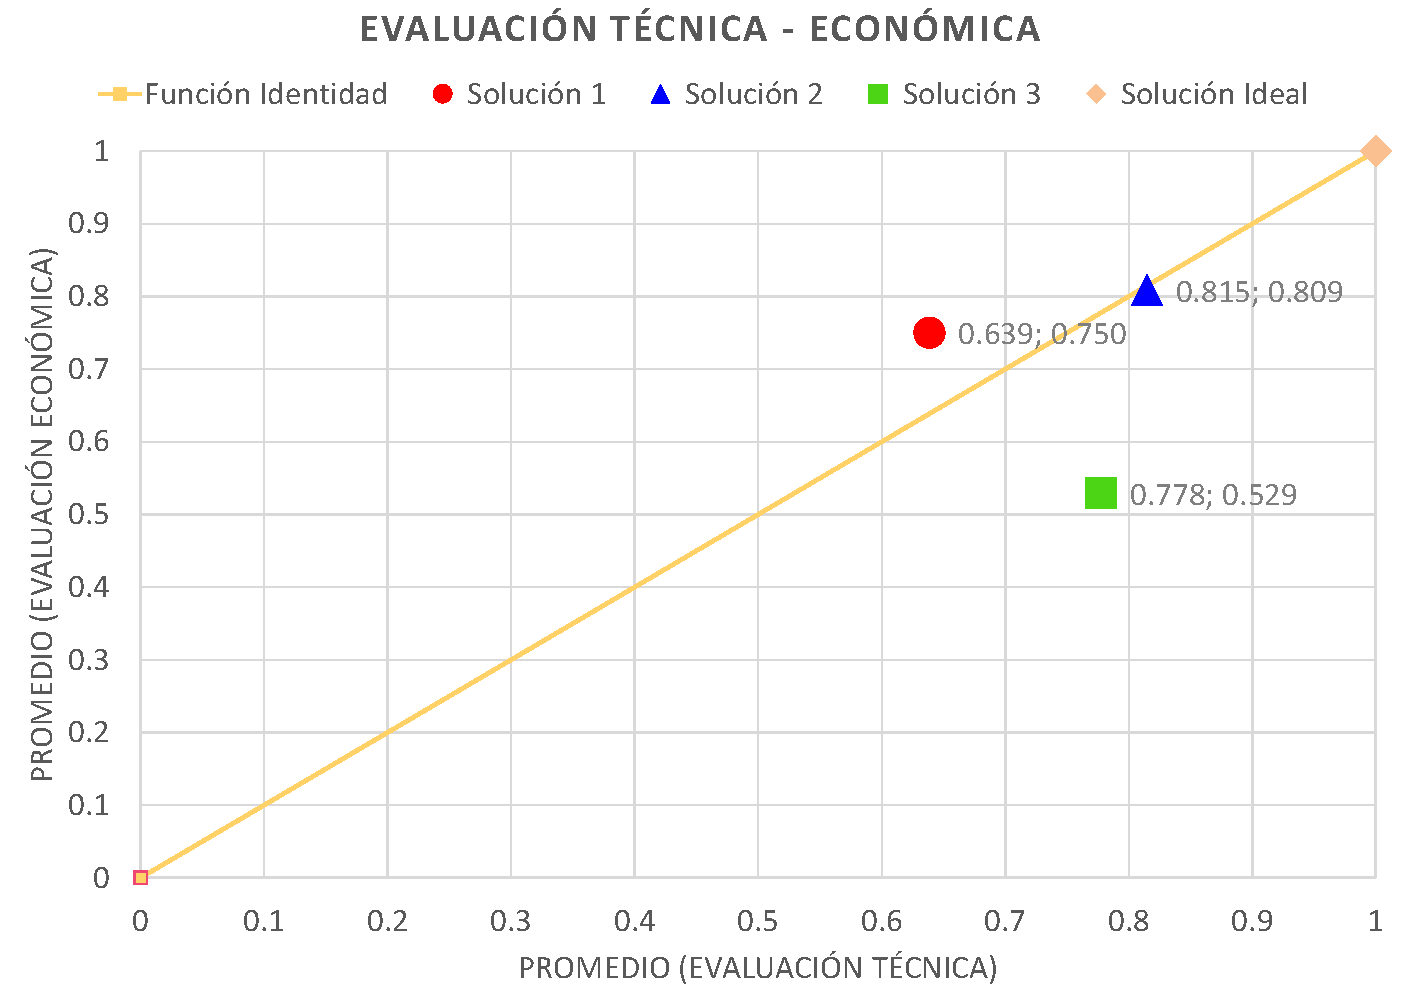
\includegraphics[width=0.9\textwidth]{img/comp_tecnico_economica.pdf}
	\caption[Gráfica de comparación técnico-económica de los conceptos de solución.]{Gráfica de comparación técnico-económica de los conceptos de solución. Fuente: Elaboración propia.}
	\label{fig:comp_tecnico_economica}
\end{figure}

Se observa que la solución que esta más cerca de la solución ideal es la \textbf{Solución 2}, en comparación con las otras opciones. Esta solución también demuestra un balance adecuado entre los aspectos económicos y técnicos, ya que se encuentra próxima a la línea de equilibrio ideal. Por lo tanto, elegimos esta solución como punto de partida para el diseño ingenieril, el cual será explorado en detalle en los siguientes capítulos.

\chapter*{Conclusiones y Recomendaciones}

\addcontentsline{toc}{chapter}{Conclusiones y Recomendaciones}

%~~~~~~~~~ Bibliography
\bibliographystyle{plainnat}
\bibliography{library}
\pagestyle{empty}
\pagenumbering{gobble}
\pagestyle{plain}
\pagenumbering{arabic}

%CAPÍTULO 1 - INTRODUCCIÓN
\chapter{Introducción}
\section{Problemática}

El presente proyecto aborda su problemática central a través de tres enfoques interrelacionados: primero, se destaca la importancia del control de calidad dentro de la industria de la moda; en segundo lugar, se identifican las ineficiencias inherentes al control de calidad tradicional; y finalmente, se subraya la creciente necesidad de automatización en el proceso de control de calidad.

\subsection*{Importancia del Control de Calidad en la Industria Textil}

Entre enero y mayo de 2022, las exportaciones de camisas, pantalones y camisetas en Perú experimentaron incrementos notables, con crecimientos del 57\%, 49\% y 31\% en valor, respectivamente. Hasta mayo de 2022, las exportaciones de confecciones alcanzaron los 759 millones de dólares americanos, marcando un aumento del 36\% en comparación con el año anterior \cite{LaCamara2022}. Estas estadísticas demuestran un crecimiento significativo en la exportación de prendas de vestir peruanas, por lo cual, es importante mantener altos estándares de calidad para satisfacer las expectativas de los mercados internacionales.

\begin{figure}[H]
	\centering
	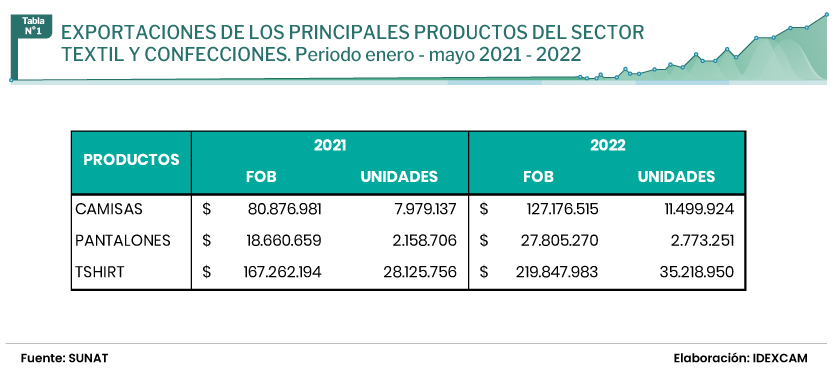
\includegraphics[width=0.8\textwidth]{img/exportaciones.jpg}
	\caption[Exportaciones peruanas de textiles: aumento en FOB y unidades, 2021 vs 2022.]{Exportaciones peruanas de textiles: aumento en FOB y unidades, 2021 vs 2022. Fuente \cite{LaCamara2022}.}
\end{figure}

El control de calidad en la industria textil es esencial para asegurar que las prendas no solo cumplan con los estándares de calidad establecidos, sino también que ofrezcan seguridad y durabilidad. Este proceso minucioso abarca diversas etapas, incluyendo la inspección de tejidos, la graduación de patrones, el corte, la costura, el acabado y finalmente, el empaquetado. Todo ello con el objetivo de garantizar que el producto final cumpla con las expectativas de los clientes. Entre los defectos más comunes que se identifican durante estas etapas se encuentran las variaciones de color, manchas, agujeros, puntadas rotas, costuras desalineadas, hilos sueltos, así como medidas incorrectas y tallas inconsistentes, tanto en los tejidos como en la construcción de las prendas \cite{TetraInspection2024}. 

\subsection*{Ineficiencias en el Control de Calidad Tradicional}

El enfoque tradicional de control de calidad, que se centra principalmente en inspecciones al final del proceso y en la implementación de correcciones a posterior, resulta en elevados costos debido a desechos y reparaciones. Este enfoque repercute negativamente en la competitividad y sostenibilidad de las empresas. Un estudio realizado por \cite{BonillaPastor2015} sobre la gestión de calidad en micro y pequeñas empresas (Mypes) del sector textil en Perú, destaca las graves consecuencias económicas y ambientales que surgen de una gestión de calidad ineficaz. Desde el punto de vista económico, los residuos y desperdicios producidos por procesos ineficientes constituyen un gasto promedio del 7.4\% en relación con el costo total de producción, lo cual impacta directamente en la competitividad y la rentabilidad de las empresas.

El control de calidad manual, como se observa en la Figura \ref{fig:insp_manual}, es ampliamente utilizada en procesos de producción debido a su relativa facilidad y la no necesidad de equipos técnicos especializados. Sin embargo, enfrenta desafíos significativos debido a factores humanos como los que se detallan en la Tabla \ref{tab:eficiencia_inspección}. Dichos factores inciden directamenteb en la efectividad del control de calidad manual, elevando potencialmente la incidencia de errores en la evaluación de la calidad. Investigaciones referenciadas en el estudio de \cite{KujawinskaVogt2015} revelan que, en tareas de inspección simples, la tasa de error puede fluctuar entre un 3\% y un 30\%, dependiendo de la índole de la tarea y las condiciones en que se efectúa la inspección.

\begin{figure}[H]
	\centering
	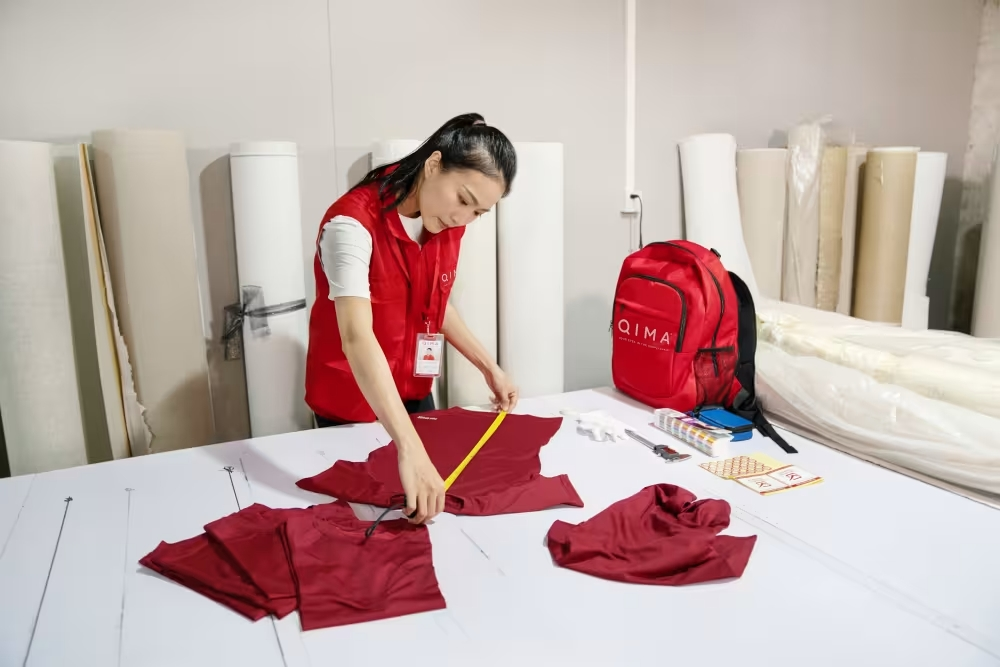
\includegraphics[width=0.65\textwidth]{img/insp_manual.jpg}
	\caption[Inspección manual de prendas de vestir.]{Inspección manual de prendas de vestir. Fuente: \cite{qimaProcedimientosInspeccin}.}
	\label{fig:insp_manual}
\end{figure}

\begin{table}[H]
	\centering
	\caption[Factores que afectan la eficiencia de la inspección visual.]{Factores que afectan la eficiencia de la inspección visual. Fuente: \cite{KujawinskaVogt2015}.}
	\begin{tabular}{|p{10em}|p{18em}|}
		\hline
		\textbf{Factors} & \textbf{Examples} \bigstrut\\
		\hline
		Technical & {Type of defects; Defect visibility; Quality level; Standards (tests); Control automation;  Other} \bigstrut\\
		\hline
		Psychophysical & Age;  Sex;  Observation  skills;  Experience;  Temperament;  Creativity;  Other \bigstrut\\
		\hline
		Organizational & Training;  Scope  of  decision  making; Feedback;  Precise  instructions;  Other \bigstrut\\
		\hline
		Workplace environment & {Light; Noise; Temperature; Work time; Workstation organization; Other} \bigstrut\\
		\hline
		Social & {Team communication;  Pressure;  Isolation; Other} \bigstrut\\
		\hline
	\end{tabular}%
	\label{tab:eficiencia_inspección}%
\end{table}%

\subsection*{Necesidad de Mejora y Automatización}

La integración de la Inteligencia Artificial (IA) en el control de calidad de la industria textil y de la moda ha introducido métodos avanzados para la inspección de calidad, desde la producción hasta la revisión final de las prendas. Esta innovación mejora significativamente la eficiencia y precisión, minimizando los errores humanos y los costos de producción, mientras asegura la adherencia a estándares de calidad elevados \cite{TextileLearner}. La Tabla \ref{tab:visual_vs_automated} resume la comparación entre inspección visual humana y la inspección automatizada. Estas limitaciones subrayan la necesidad de un proceso de inspección más automatizado y preciso para reducir errores y mejorar la eficiencia \cite{Islam2006ASuitable}.

\begin{table}[H]
	\centering
	\caption[Inspección visual versus inspección automatizada.]{Inspección visual versus inspección automatizada \cite{Islam2006ASuitable}.}
	\begin{tabular}{|p{13em}|c|c|}
		\hline
		\textbf{Inspection Type} & {\textbf{Visual}} & \textbf{Automated} \bigstrut\\
		\hline
		Fabric Types & 100\% & \multicolumn{1}{c|}{70\%} \bigstrut\\
		\hline
		Defect Detection Rate & 70\%  & 80\%+ \bigstrut\\
		\hline
		Reproducibility & 50\%  & 90\%+ \bigstrut\\
		\hline
		Objective Defect Judgment & 50\%  & {100\%} \bigstrut\\
		\hline
		Statistics Ability & 0\%   & 95\%+ \bigstrut\\
		\hline
		Inspection Speed & {30 m/min} & {120 m/min} \bigstrut\\
		\hline
		Response Type & 50\%  & {80\%} \bigstrut\\
		\hline
		Information Content & 50\%  & 90\%+ \bigstrut\\
		\hline
		Information Exchange & 20\%  & 90\%+ \bigstrut\\
		\hline
	\end{tabular}%
	\label{tab:visual_vs_automated}%
\end{table}%

La automatización en la detección de defectos mediante visión artificial es crucial en manufactura, mejorando la consistencia y reduciendo errores humanos. La inspección óptica automatizada, impulsada por aprendizaje profundo y machine learning, supera los métodos manuales, ofreciendo eficiencia y precisión. Esto facilita la identificación rápida y confiable de defectos, elevando la calidad del producto y disminuyendo costos y tiempos de producción. La utilización de redes neuronales convolucionales para la extracción de características mejora la adaptabilidad y eficiencia de la inspección, siendo clave para el avance en manufactura. \cite{SanchezRomero2023}.

\section{Propuesta de Solución}

\section{Objetivos}

El proyecto presenta un objetivo general del cual surgen \ref{lst:objetivos_especificos} objetivos específicos para lograr el cumplimiento del objetivo general.

\subsection{Objetivo General}

Desarrollar un sistema integrado para el control de calidad de prendas de vestir, que combine tecnologías de visión artificial y detección de metales para inspeccionar cada prenda de manera individual, asegurando su conformidad con los estándares de calidad establecidos en la ficha técnica de la prenda, tales como la ausencia de defectos visibles, la precisión en las medidas de talla y la detección de elementos metálicos extraños.

\subsection{Objetivos Específicos}

\begin{enumerate}
	\setlength\itemsep{-0.5em}
	\item Realizar una revisión bibliográfica (estado del arte) que permita definir los requerimientos del diseño del sistema y todo lo concerniente al diseño conceptual.
	
	\item Definir las exigencias específicas que debe cumplir el sistema para lograr el objetivo principal.
	
	\item Seguir la metodología de diseño basada en la norma VDI 2206 para el diseño mecatrónico completo del sistema.
	
	\item Diseñar un subsistema mecánico que permita transportar las prendas de vestir a través de los distintos módulos del sistema.
	
	\item Diseñar un subsistema de inspección por procesamiento de imágenes para realizar la medición de la talla de las prendas y realizar la verificación según la ficha técnica de la prenda.
	
	\item Diseñar un subsistema de detección de metales que examine cada prenda para identificar y alertar sobre la presencia de agujas, alfileres o cualquier otro elemento metálico extraño, garantizando así la seguridad del producto final.
	
	\item Desarrollar una interfaz intuitiva para mostrar resultados de detección de calidad de prendas, incluyendo visualización de defectos, mediciones de tallas e identificación de metales
	
	\item Seleccionar el concepto de solución óptimo basados en los criterios técnicos y económicos, según la norma VDI 2225.
	
	\item Estimar un costo de fabricación de un prototipo a partir de los componentes seleccionados.
	
	\label{lst:objetivos_especificos}
\end{enumerate}

\section{Metodología}
% BENDEZU_LEDESMA_JORGE_DISEÑO_PROTOTIPO_DRON

Para el desarrollo del presente trabajo se emplearan adaptaciones de las metodologías diseñadas por la VDI (Asociación Alemana de Ingenieros). Entre ellas, se utilizar una adaptación de la metodología VDI 2206 \cite{VDIVDE2206_2021} y de la metodología VDI 2221 \cite{VDI2221_2019} para el diseño conceptual, el cual consistirá en las siguientes etapas: Elaboración de lista de requerimientos, Elaboración de un diagrama de funciones y Elaboración de una matriz morfológica (con 3 soluciones). Posteriormente se seguirá una adaptación de la metodología VDI 2225 \cite{VDI2225_series} para realizar un análisis técnico y económica de las soluciones.

De ese modo, los Capítulos 1 y 2 se enfocaran en a comprender la problemática de la investigación. El Capítulo 1 aborda una investigación preliminar para contextualizar el problema, identificar los enfoques de la problemática y definir el alcance de la solución. El Capítulo 2, por su parte, examina el estado actual de la tecnología para establecer un marco de referencia que permita evaluar la viabilidad del proyecto, con el fin de determinar parámetros y características relevantes para el sistema de control de calidad en prendas de vestir.

En el Capítulo 3, se desarrollan los procesos de la metodología correspondientes para diseñar la estructura de funciones y el concepto de solución. Utilizando la lista de requerimientos, se abstrae el problema para obtener una comprensión amplia de las funciones necesarias, lo que guía el diseño mecánico y eléctrico inicial y ayuda a determinar los sensores, actuadores y fuentes de energía necesarios. A partir de esta estructura, se crea una matriz morfológica que facilita la combinación de distintas alternativas de solución, culminando en la definición precisa de los objetivos de diseño e implementación. Además, se realizará una ponderación de los conceptos de solución a través de un análisis técnico-económico con el objetivo de obtener un concepto de solución óptimo.

Por último, en los capítulos subsecuentes se realizaran los siguientes partes del trabajo:

\begin{itemize}
	\setlength\itemsep{-0.5em}
	\item Realización de cálculos mecánicos, electrónicos y de control necesarios para determinar las características de la máquina.
	\item Se va a seleccionar (o diseñar) un modelo de inteligencia artificial para realizar la labor de la visión artificial del sistema, además, se va a buscar, o en su defecto, se va a crear un dataset para entrenar un modelo de inteligencia artificial.
	\item Verificación de las partes mecánicas por medio de software de elementos finitos.
	\item Elaboración de planos y estimación de costos de fabricación.
\end{itemize}

\section{Alcance de la Investigación}

Este trabajo se enfoca en el diseño de un sistema a través del dimensionamiento detallado de cada uno de sus componentes. El objetivo principal es lograr que el sistema opere de manera autónoma. En otras palabras, se busca reducir la intervención humana al mínimo necesario. Esta intervención se limita a tareas como la inserción de la prenda a verificar en el sistema, el ingreso de señales de control y la posterior retirada de la prenda ya evaluada. Es importante destacar que los requisitos definidos para este proyecto, desarrollados a lo largo de la investigación, están orientados a un entorno no industrial. Además, se señala que el prototipo busca alcanzar un Nivel 4 de Madurez Tecnológica (TRL4), mediante simulaciones que se llevarán a cabo tanto en software como a través de un Producto Mínimo Viable (MVP) en un entorno de laboratorio controlado.

Para concluir, esta tesis presentará todos los cálculos de diseño necesarios, así como los planos mecánicos y electrónicos, los materiales escogidos para el proyecto, y los diagramas de flujo que explican la operación y control del sistema.

%CAPÍTULO 2 - ESTADO DEL ARTE
\chapter{Estado del Arte}
\label{Estado del Arte}
En este capítulo se presenta una revisión de trabajos de investigación, sistemas comerciales y patentes relacionados al control de calidad automático de prendas de vestir. Asimismo, se presentan las tecnologías involucradas a la detección de defectos mediante visión artificial, detección de metales, y luz UV para detectar manchas de grasa en las prendas de vestir.

% \section{Sistema Integrado de Control de Calidad de Prendas}

\subsection{Investigaciones Académicas}

\subsubsection{System of error detection in the manufacture of garments using artificial vision}

El sistema desarrollado la investigación \cite{Moreno2017} consiste en un sistema de visión artificial implementado para detectar errores en la etapa de corte durante el proceso de fabricación de prendas en la industria textil. Utiliza un sistema embebido Raspberry Pi 3, equipado con el sistema operativo basado en Linux Raspbian y el compilador OpenCV para el desarrollo de códigos de visión por computadora. Este sistema, que se muestra en \ref{fig:luz_sistema}, logra segmentar perfectamente las prendas independientemente del color que se les haya dado en procesos anteriores, gracias a la implementación de un fondo dinámico opaco compuesto por LEDs RGB que cambian de color dependiendo del contraste con la prenda.

El algoritmo principal del sistema inicia con la captura de la imagen de la prenda, seguido por el promedio de cada canal de la imagen completa (rojo, verde y azul). Luego, se cambia el color del fondo basándose en el color que menos presencia tenga en la imagen, utilizando combinaciones de colores primarios en los LEDs RGB para minimizar el consumo de corriente. Finalmente, se captura una nueva imagen con el fondo bien contrastado con la prenda para verificar el contraste correcto.

\begin{figure}[H]
	\centering
	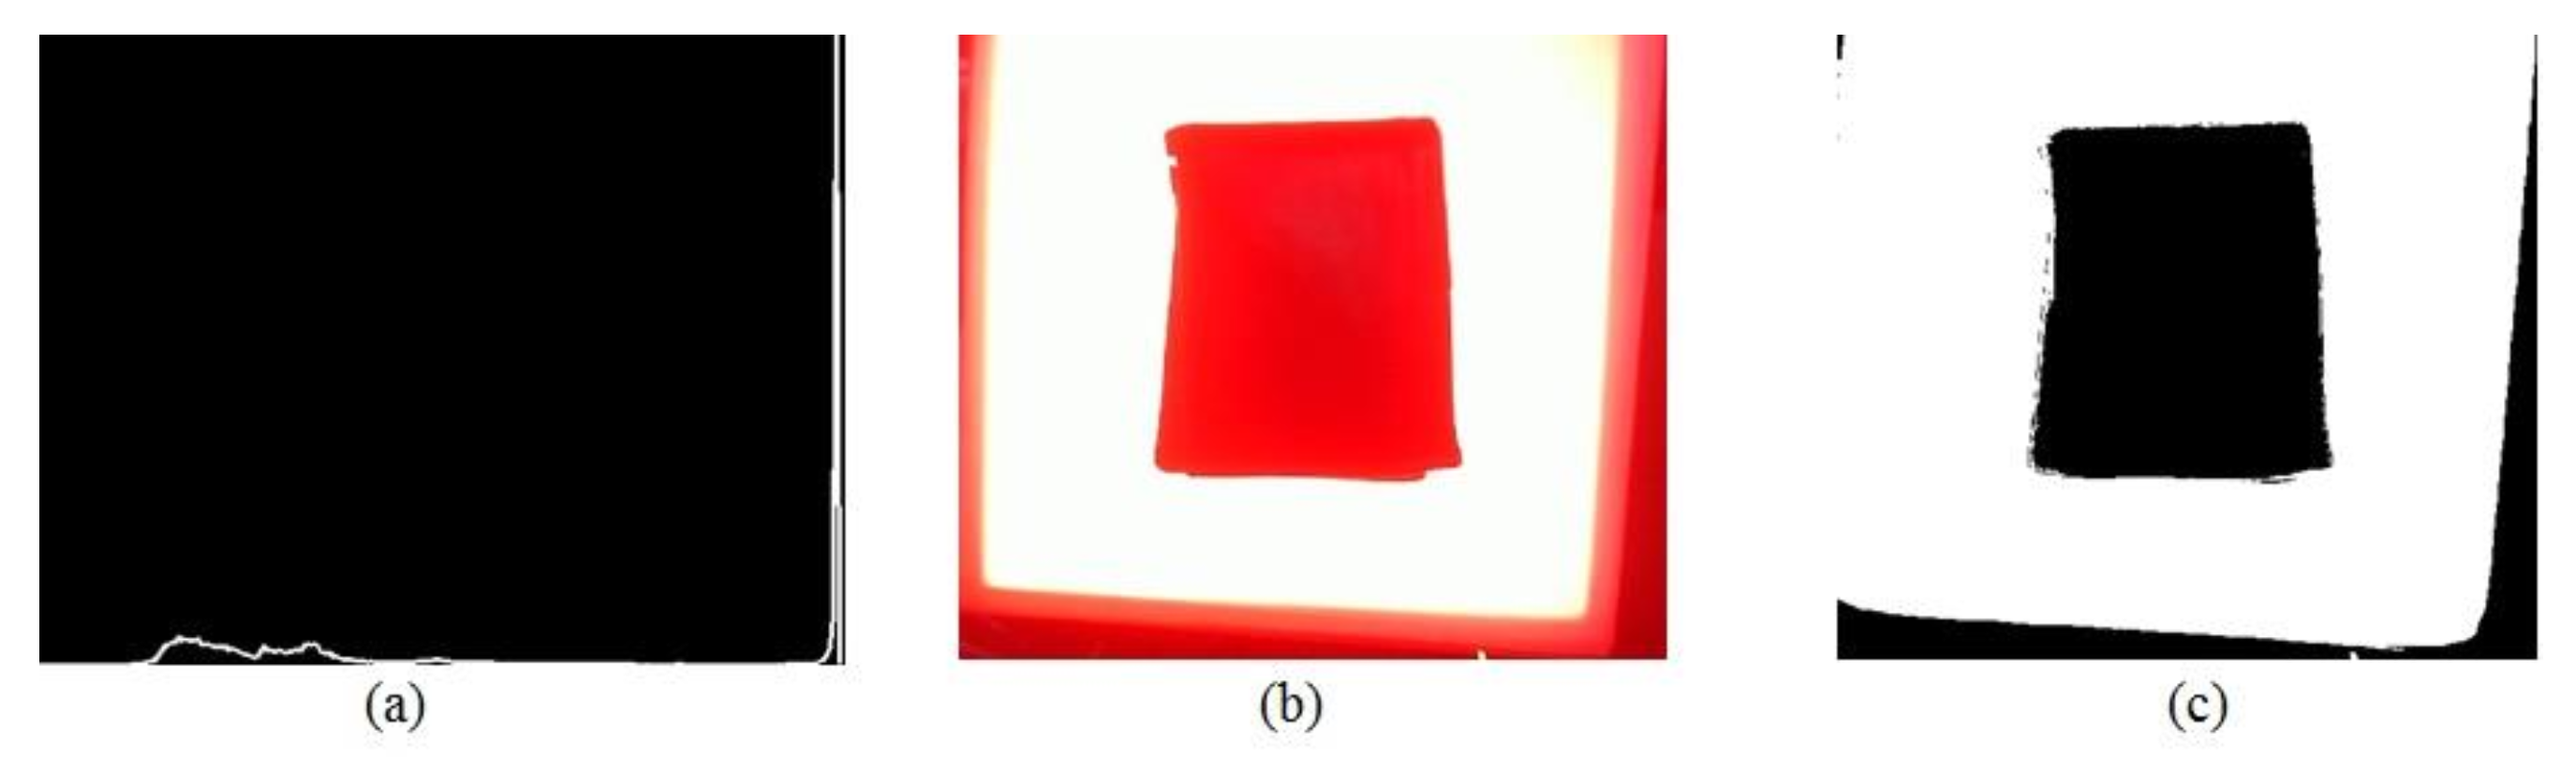
\includegraphics[width=0.8\textwidth]{img/luz_sistema.png}
	\caption[Sistema de visión artificial con fondo dinámico.]{Sistema de visión artificial con fondo dinámico \cite{Moreno2017}.}
	\label{fig:luz_sistema}
\end{figure}

\subsubsection{Using object detection technology to identify defects in clothing for blind people}

En la investigación \cite{Rocha2023} se muestra como la tecnología de detección de objetos, específicamente la arquitectura You Only Look Once (YOLO), ha sido aplicada de manera innovadora para ayudar a las personas ciegas a identificar defectos, como manchas o agujeros, en su ropa. Este enfoque utiliza un sistema de detección de defectos basado en el aprendizaje profundo para categorizar y detectar estas imperfecciones en prendas de vestir, lo que representa un paso importante hacia la mejora de la autonomía y la confianza de las personas ciegas en la selección de su vestimenta. El sistema propuesto en este estudio se basa en la recolección de un conjunto de datos específico de ropa con defectos, el cual es utilizado para entrenar y evaluar el sistema. La metodología empleada para optimizar el sistema de detección de defectos incluye aumentar el conjunto de datos con nuevos defectos, condiciones de iluminación y fondos, introducir la ampliación de datos y la clasificación de defectos, demostrando ser eficaz y adecuado para diferentes condiciones de detección de defectos desafiantes.

El trabajo futuro en este campo se centra en la creación de una aplicación móvil y un sistema mecatrónico, como un armario automático, que incorpore los algoritmos y metodologías desarrolladas. Esto no solo pone de manifiesto la utilidad práctica de la tecnología de detección de objetos para la comunidad ciega, sino que también abre la puerta a aplicaciones automáticas que pueden facilitar aún más la gestión del vestuario por parte de las personas con discapacidad visual, proporcionando una herramienta de apoyo esencial para su independencia y confianza en la vida cotidiana. Este enfoque innovador destaca el potencial de las tecnologías de visión por computadora en la asistencia y mejora de la calidad de vida de las personas con discapacidades visuales.

\begin{figure}[H]
	\centering
	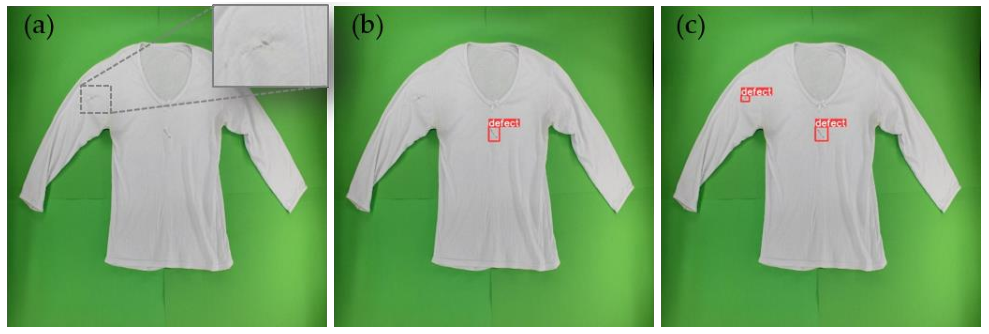
\includegraphics[width=0.9\textwidth]{img/example_YOLO.pdf}
	\caption[Defecto ignorado por YOLOv5m6, detectado tras la ampliación de datos.]{Defecto ignorado por YOLOv5m6, detectado tras la ampliación de datos desarrolada por \cite{Rocha2023}: (a) imagen original, (b) imagen predicha por el modelo YOLOv5m6 sin ampliación, y (c) imagen predicha por el modelo YOLOv5m6 con ampliación.}
	\label{fig:example_YOLO}
\end{figure}

\subsubsection{Automatic Measurement of Garment Sizes Using Image Recognition}

El documento presenta una innovadora metodología para medir automáticamente las tallas de prendas de vestir utilizando tecnología de reconocimiento de imágenes mediante el dispositivo que se muestra en la Figura \ref{fig:Automatic_Measurement}. Al enfrentar el problema de altas tasas de devolución en la moda en línea, debido a las inconsistencias en las tallas entre diferentes marcas y fabricantes, este estudio propone una solución tecnológica que combina el diseño de un conjunto de equipos especializados para capturar imágenes de prendas extendidas y un enfoque de medición automática basado en plantillas de prendas. Estas plantillas permiten identificar el tipo de prenda y puntos de características clave para calcular sus tallas. Este método ofrece una herramienta útil y eficiente para la medición de prendas, mostrando resultados precisos que satisfacen los requisitos de la industria del vestido, y tiene el potencial de mejorar significativamente la experiencia de compra en línea al reducir la tasa de devoluciones gracias a una estandarización en la medición de tallas \cite{Li2017AutomaticMeasurement}.

\begin{figure}[H]
	\centering
	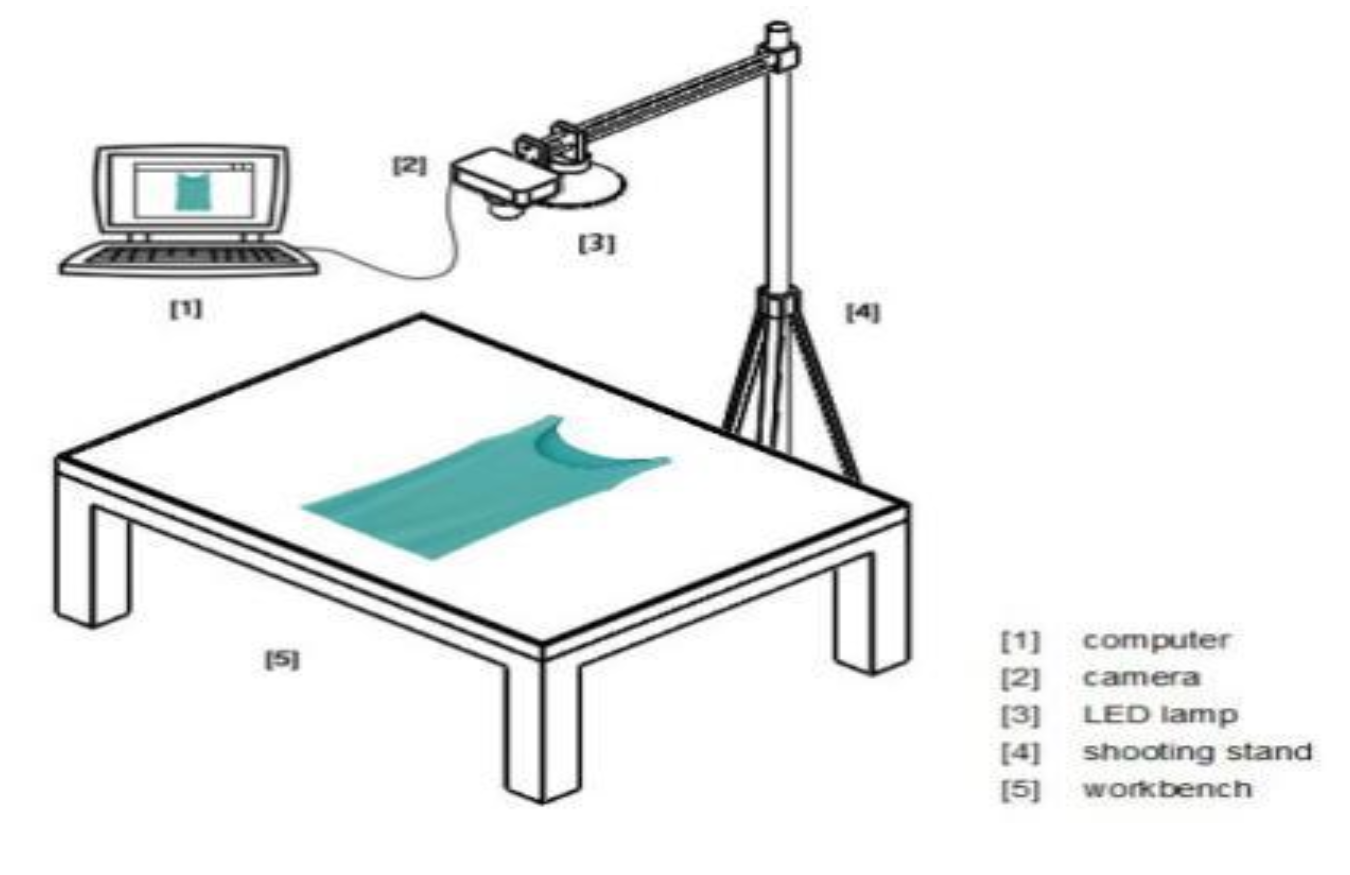
\includegraphics[width=0.6\textwidth]{img/Automatic_Measurement.png}
	\caption[Diseño de un dispositivo para medición automática de tallas de prendas mediante reconocimiento de imágenes]{Diseño de un dispositivo para medición automática de tallas de prendas mediante reconocimiento de imágenes \cite{Li2017AutomaticMeasurement}.}
	\label{fig:Automatic_Measurement}
\end{figure}

\subsection{Productos Comerciales}

\subsubsection{Handheld Needle Detector ON-30}

En el contexto de la detección de metales en la industria textil, el Detector de Agujas Portátil ON-30 de Oshima, que se muestra en la Figura \ref{fig:oshima_on_30} se presenta como una herramienta eficaz. Este dispositivo, alimentado por baterías AA y basado en inducción magnética, se destaca por su capacidad para identificar con precisión objetos metálicos pequeños. Su diseño compacto y la implementación de alarmas visuales y sonoras facilitan su uso en diversas situaciones, ofreciendo una solución práctica para garantizar la seguridad en los procesos de producción textil \cite{oshimaEfficientHandheld}. Las características de este producto se observan en el Cuadro \ref{tab:specs_ON_30}.

\begin{figure}[H]
	\centering
	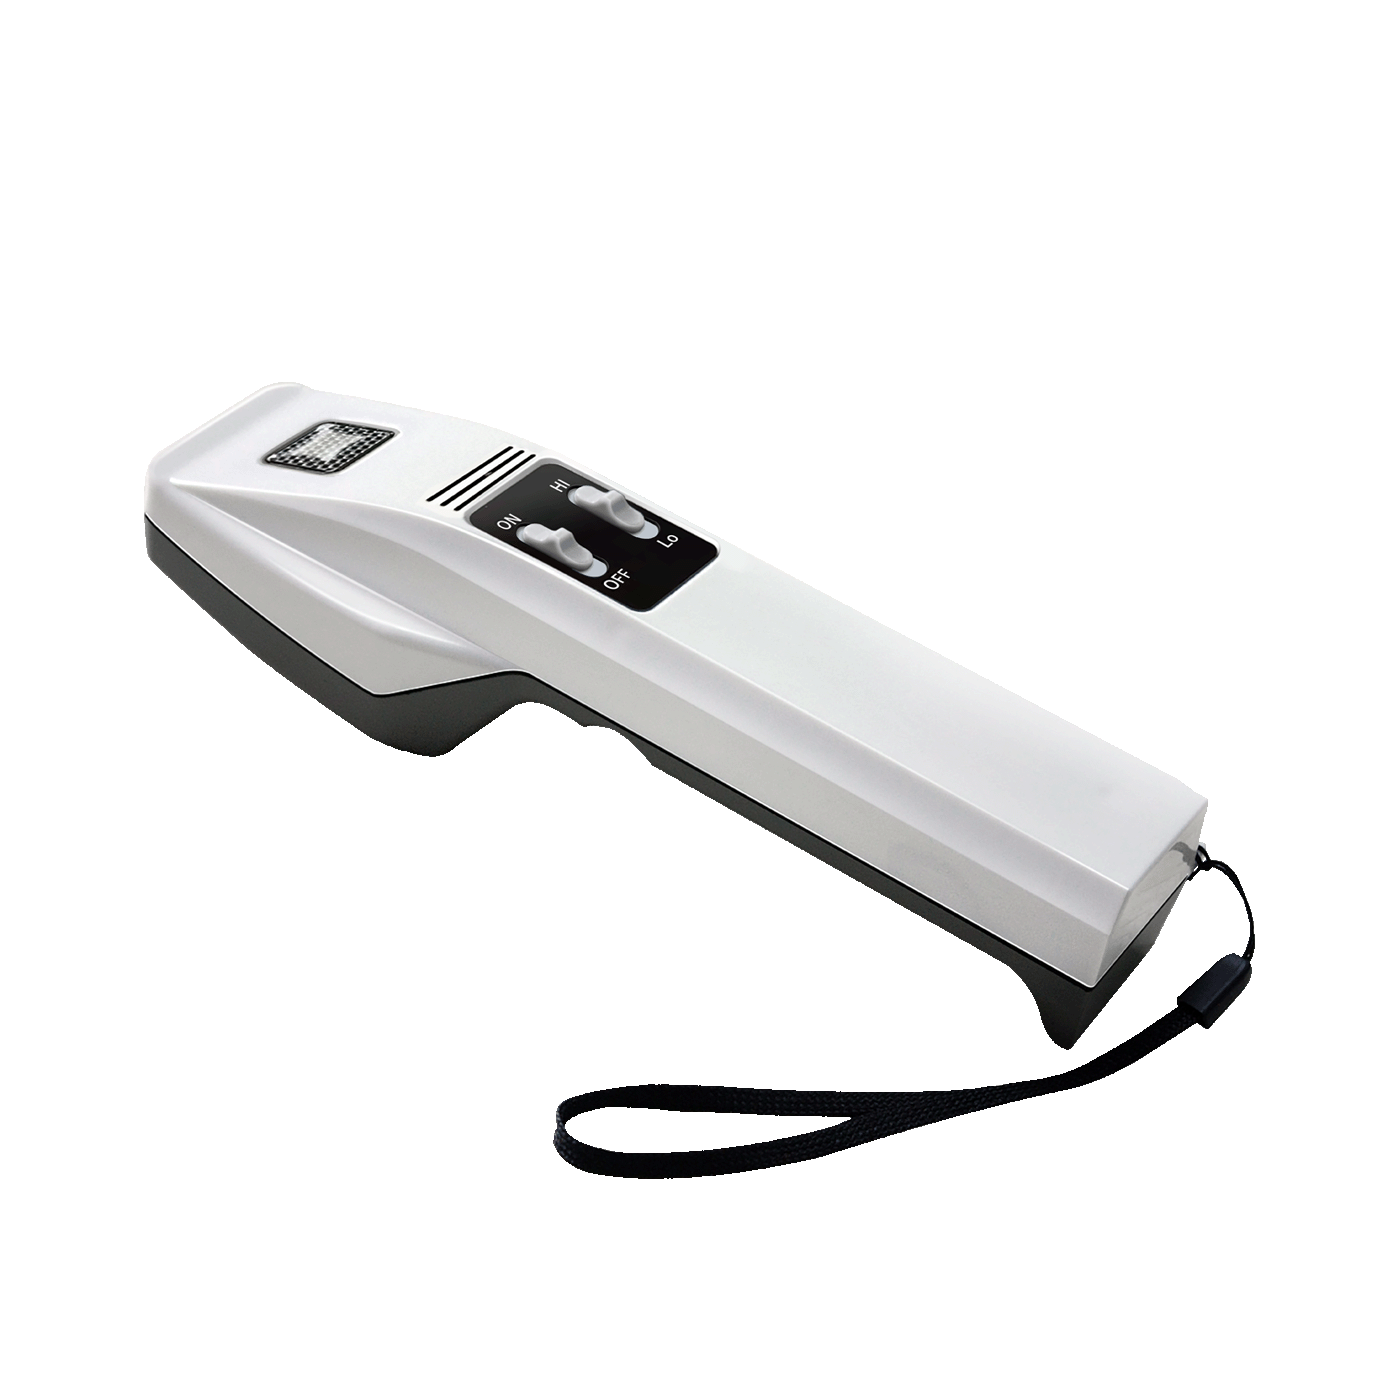
\includegraphics[width=0.4\textwidth]{img/oshima_on_30.png}
	\caption{Detector de Agujas Portátil ON-30 de Oshima.}
	\label{fig:oshima_on_30}
\end{figure}

\begin{table}[H]
	\caption{Especificaciones del Modelo ON-30.}
	\begin{tabularx}{\textwidth}{|l|X|}
		\hline
		\textbf{Característica} & \textbf{Especificación} \\ \hline
		Modelo & ON-30 \\ \hline
		Fuente de Alimentación & Batería 6F22-9V, corriente de reposo del LED <5mA. Alarma de sonido y luz. Corriente dinámica <30mA, corriente dinámica de la alarma de vibración <60mA, ahorro de energía. \\ \hline
		Sensibilidad & La inspección cercana puede detectar una bola de hierro de 0.5 mm, una bola de hierro de 1.2 mm de diámetro hasta una altura de 10 mm. La máxima sensibilidad puede detectar una bola de hierro de 0.8 mm de diámetro, un pasador de ruptura de 0.7 x 20 de diámetro hasta una altura de 50 mm. \\ \hline
		Método de Detección & Inducción magnética \\ \hline
		Espacio de Detección (mm) & 70x55 \\ \hline
		Alarma & Zumbador, lámpara \\ \hline
		Dimensiones LxAxA (mm) & 195x58x50 \\ \hline
		Volumen del Empaque LxAxA (mm) & 250x100x55 \\ \hline
		Peso Neto/Peso Bruto (kg) & 0.212/0.35 \\ \hline
	\end{tabularx}
	\label{tab:specs_ON_30}
\end{table}

\subsubsection{Digital Conveyor Needle Detectors ON-688CD6S/688CDD6S}

Los detectores de agujas para cinta transportadora ON-688CD6S/688CDD6S de OSHIMA incorporan sensores de 10 puntos para una mayor sensibilidad y confiabilidad, con ajuste de sensibilidad en tres niveles para diferentes necesidades de detección. Su interfaz de pantalla táctil facilita su uso, y la máquina es capaz de conectarse a datos, contabilizar productos, y calibrarse automáticamente cada dos horas \cite{oshimaOSHIMAGarment}. Las especificaciones de estos modelos se muestran en la Tabla \ref{tab:specs_ON-688CD6S/688CDD6S}.

\begin{figure}[H]
	\centering
	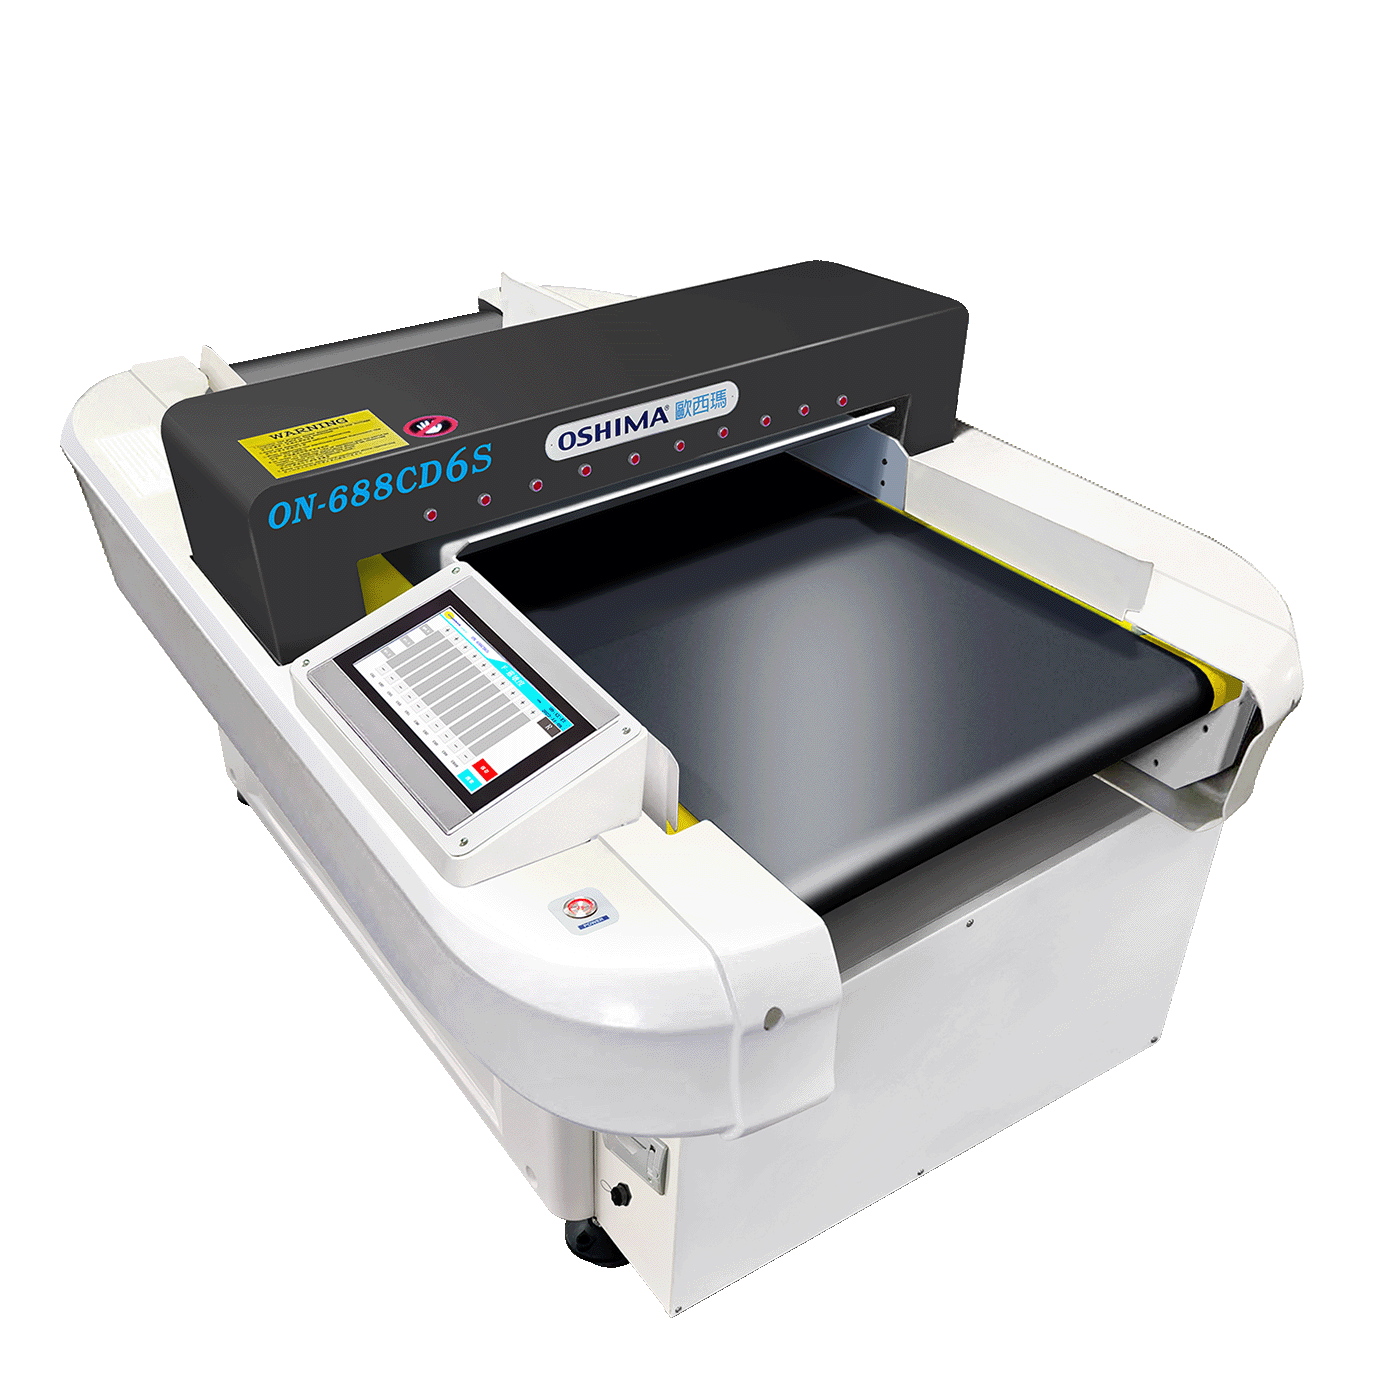
\includegraphics[width=0.5\textwidth]{img/oshima_conveyor.png}
	\caption{Detectores de Agujas para Cinta Transportadora Digital ON-688CD6S/688CDD6S.}
	\label{fig:oshima_conveyor}
\end{figure}

\begin{table}[H]
	\caption{Especificaciones de los modelos ON-688CD6S/688CDD6S.}
	\begin{tabularx}{\textwidth}{|X|X|X|}
		\hline
		\multirow{2}{*}[2pt]{\textbf{Característica}} & \multicolumn{2}{c|}{\textbf{Especificaciones}} \\ \cline{2-3}
		& \textbf{ON-688CD6S} & \textbf{ON-688CDD6S} \\
		\hline
		Detecting tower & Single tower & Double tower \\
		\hline
		Detective height (mm) & 100 & 100 \\
		\hline
		Detective width (mm) & 600 & 600 \\
		\hline
		Effective detecting Height (mm) & 90 & 90 \\
		\hline
		Power supply & 1P AC220V 50/60Hz & 1P AC220V 50/60Hz \\
		\hline
		Rate (kW) & 0.2 & 0.2 \\
		\hline
		Detective capability of iron ball (mm) & Fe 0.8/1.0/1.2 & Fe 0.8/1.0/1.2 \\
		\hline
		Sensitivity adjustment & Level adjustment & Level adjustment \\
		\hline
		Conveyor speed (m/min) & 32 & 32 \\
		\hline
		Detection method & Magnet & Magnet \\
		\hline
		Alarm & Automatic buzzer and alarm indicator light, the conveyor rewinding function & Automatic buzzer and alarm indicator light, the conveyor rewinding function \\
		\hline
		Dimensions LxWxH (mm) & 1720X1100X920 & 1820X1180X1100 \\
		\hline
		Packaging volume LxWxH (mm) & 2160X1060X920 & 2330X1130X1100 \\
		\hline
		N.W/G.W (kg) & 280/380 & 420/570 \\
		\hline
	\end{tabularx}
	\label{tab:specs_ON-688CD6S/688CDD6S}
\end{table}

\subsubsection{AI-Driven Measurement Checking Machine}

Este desarrollo tecnológico, el cual se muestra en la Figura \ref{fig:inspection_machine} de la empresa Dongguan Yunji Zhihui Technology facilita la automatización de procesos previamente manuales, por lo que augura reducciones significativas en los costos laborales y mejoras en el control de calidad \cite{RMG2021AIGarment}. Las especificaciones de este sistema se muestran en la Tabla \ref{tab:spec_inspection_machine}.

\begin{figure}[H]
	\centering
	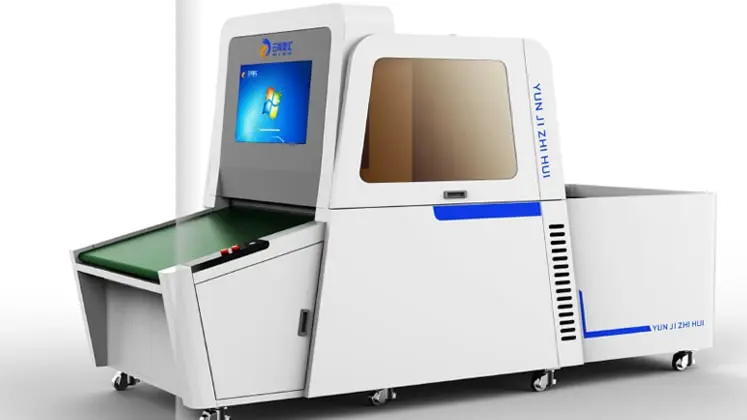
\includegraphics[width=0.7\textwidth]{img/inspection_machine.png}
	\caption[Máquina de chequeo de medidas conducido por IA.]{Máquina de chequeo de medidas conducido por IA. Fuente: \cite{RMG2021AIGarment}.}
	\label{fig:inspection_machine}
\end{figure}

\begin{table}[h!]
	\centering
	\caption[Características cuantitativas del sistema de inspección de prendas con IA.]{Características cuantitativas del sistema de inspección de prendas con IA. Fuente: Elaboración propia.}
	\begin{tabular}{|l|l|}
		\hline
		\textbf{Característica} & \textbf{Valor} \\ \hline
		Dimensiones medidas por prenda & 15 dimensiones \\ \hline
		Tiempo por artículo & Máximo 6 segundos \\ \hline
		Capacidad de procesamiento & 4800 camisetas en 480 minutos \\ \hline
		Precisión de medición & Error dentro de ±1 mm \\ \hline
		Exactitud de detección & Hasta el 99.5\% \\ \hline
		Adaptabilidad & Ajuste según color y tela de las prendas \\ \hline
	\end{tabular}
	\label{tab:spec_inspection_machine}
\end{table}

\subsection{Patentes}

\subsubsection{US20200178632A1}
La invención \cite{us20200178632a1} describe un aparato, método y sistema de control automatizado para mejorar la inspección, medición y fabricación de prendas de vestir como se observa en la Figura \ref{fig:US20200178632A1-20200611-D00005}. Este sistema captura una imagen de la prenda la convierte en una representación digital que puede enviarse y almacenarse en una base de datos. Esta información digital se utiliza para recrear prendas ideales con medidas y patrones reproducibles. Además, el sistema permite comparaciones con imágenes ideales existentes y/o con la propia prenda para determinar si posee las dimensiones, formas, colores, texturas y tejidos correctos.

\begin{figure}[H]
	\centering
	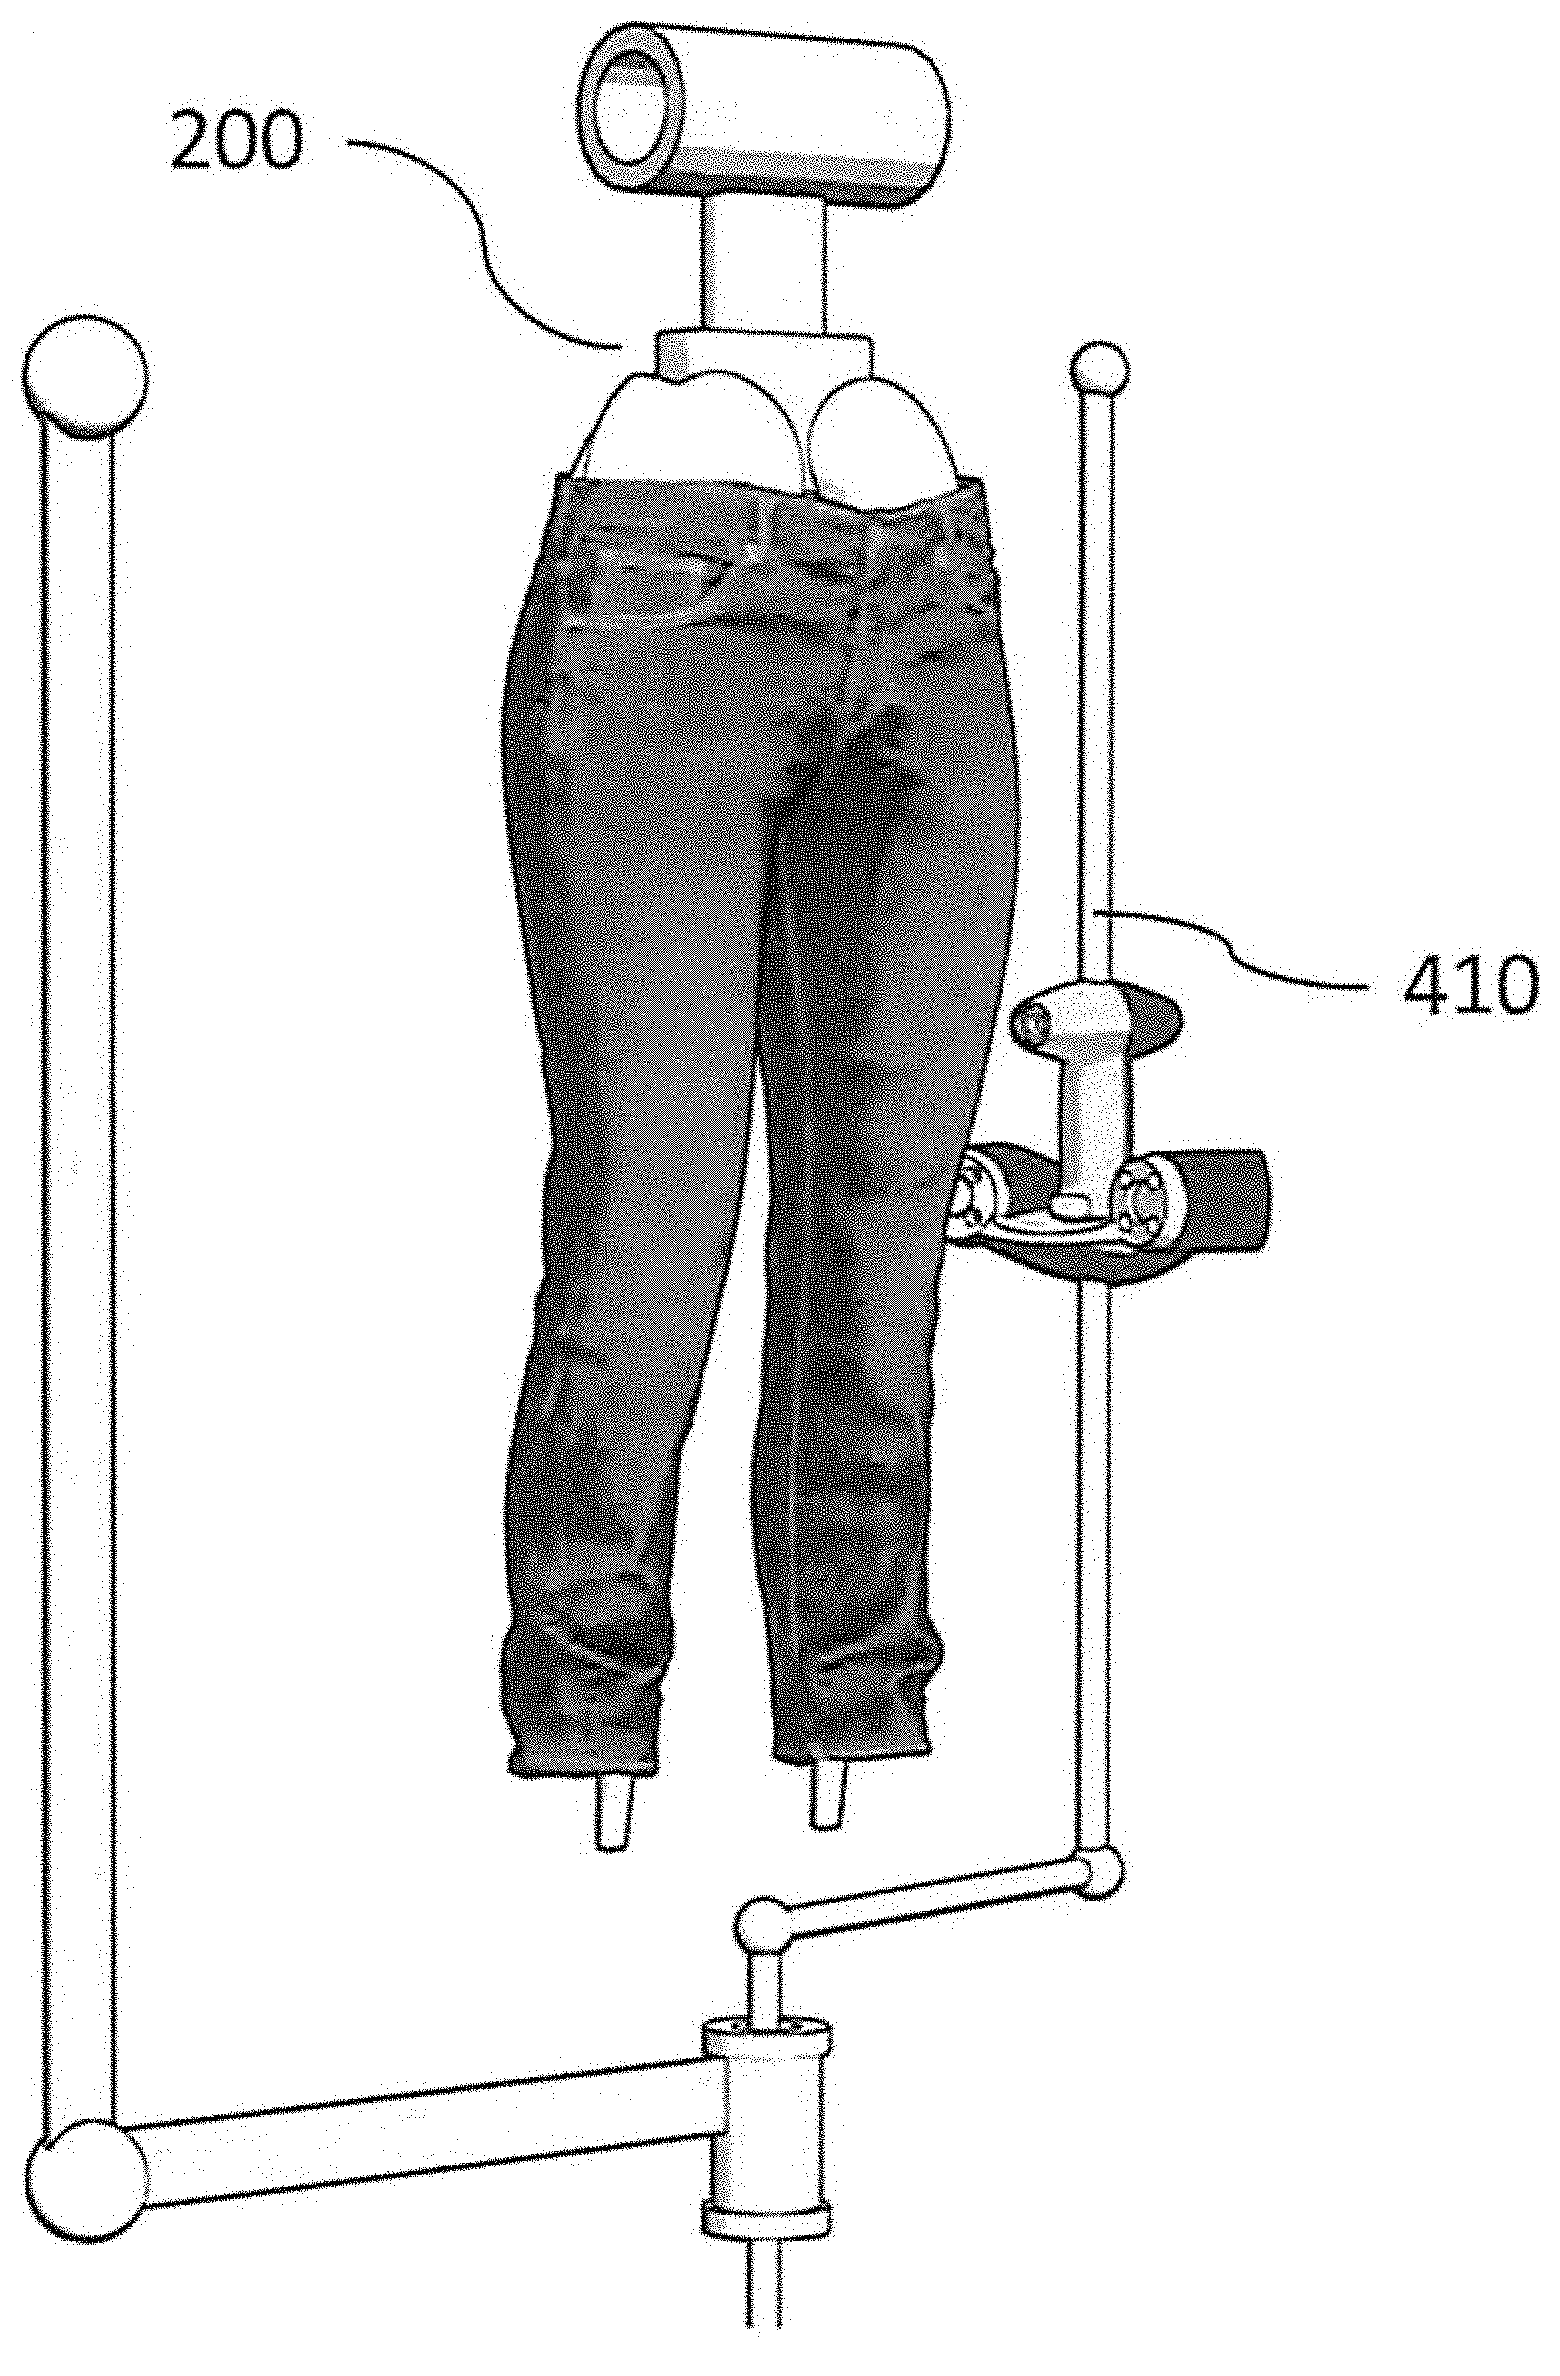
\includegraphics[width=0.3\textwidth]{img/US20200178632A1-20200611-D00005.png}
	\caption{Patente con captura de detalles en 3D.}
	\label{fig:US20200178632A1-20200611-D00005}
\end{figure}

\subsubsection{US5530652A}

La invención \cite{US5530652A} detalla un sistema que incluye técnicas de escaneo 3D (ópticas o electroópticas) para adquirir datos de escaneo dimensionales. Estos datos se procesan para la extracción de medidas y retroalimentación. La organización de los datos permite su almacenamiento y recuperación, finalizando con el control de medidas de las prendas, la fabricación y la categorización basada en la retroalimentación.

Este sistema se destaca por su capacidad para automatizar el control y la inspección de la calidad de las prendas producidas, minimizando la necesidad de contacto humano directo con los objetos, lo que facilita un análisis dimensional preciso y automatizado. La tecnología descrita en esta patente tiene potencial para revolucionar la forma en que se miden, inspeccionan y fabrican las prendas de vestir, asegurando consistencia y calidad en la producción de vestimenta.

La patente US5530652 describe un sistema automático de inspección y medición de prendas que puede crear representaciones electrónicas bidimensionales o tridimensionales de un objeto. Estas representaciones pueden ser combinadas con otras para crear una base de datos de medidas de donde se pueden generar patrones estándar para su uso en la fabricación de prendas. Además, la representación electrónica puede utilizarse para comparar el objeto fabricado con una representación ideal, determinando si las medidas del objeto se encuentran dentro de una tolerancia predeterminada respecto a la representación ideal. Se emplea un sistema de visión por máquina para capturar una imagen del objeto y convertirla en una representación digital, que luego puede agregarse a una base de datos para compilar un patrón ideal o compararse con una imagen ideal existente para verificar si el objeto tiene el tamaño correcto.

La patente aborda el desarrollo de un método y un sistema para la inspección y medición automática de prendas, con el objetivo de asegurar que las dimensiones de las prendas fabricadas se ajusten a los estándares ideales y tolerancias predefinidas. Esto facilita la creación de bases de datos de medidas que pueden utilizarse para mejorar la fabricación de prendas, asegurando una mayor precisión y consistencia en el tamaño y la calidad de las prendas producidas.

\begin{figure}[H]
	\centering
	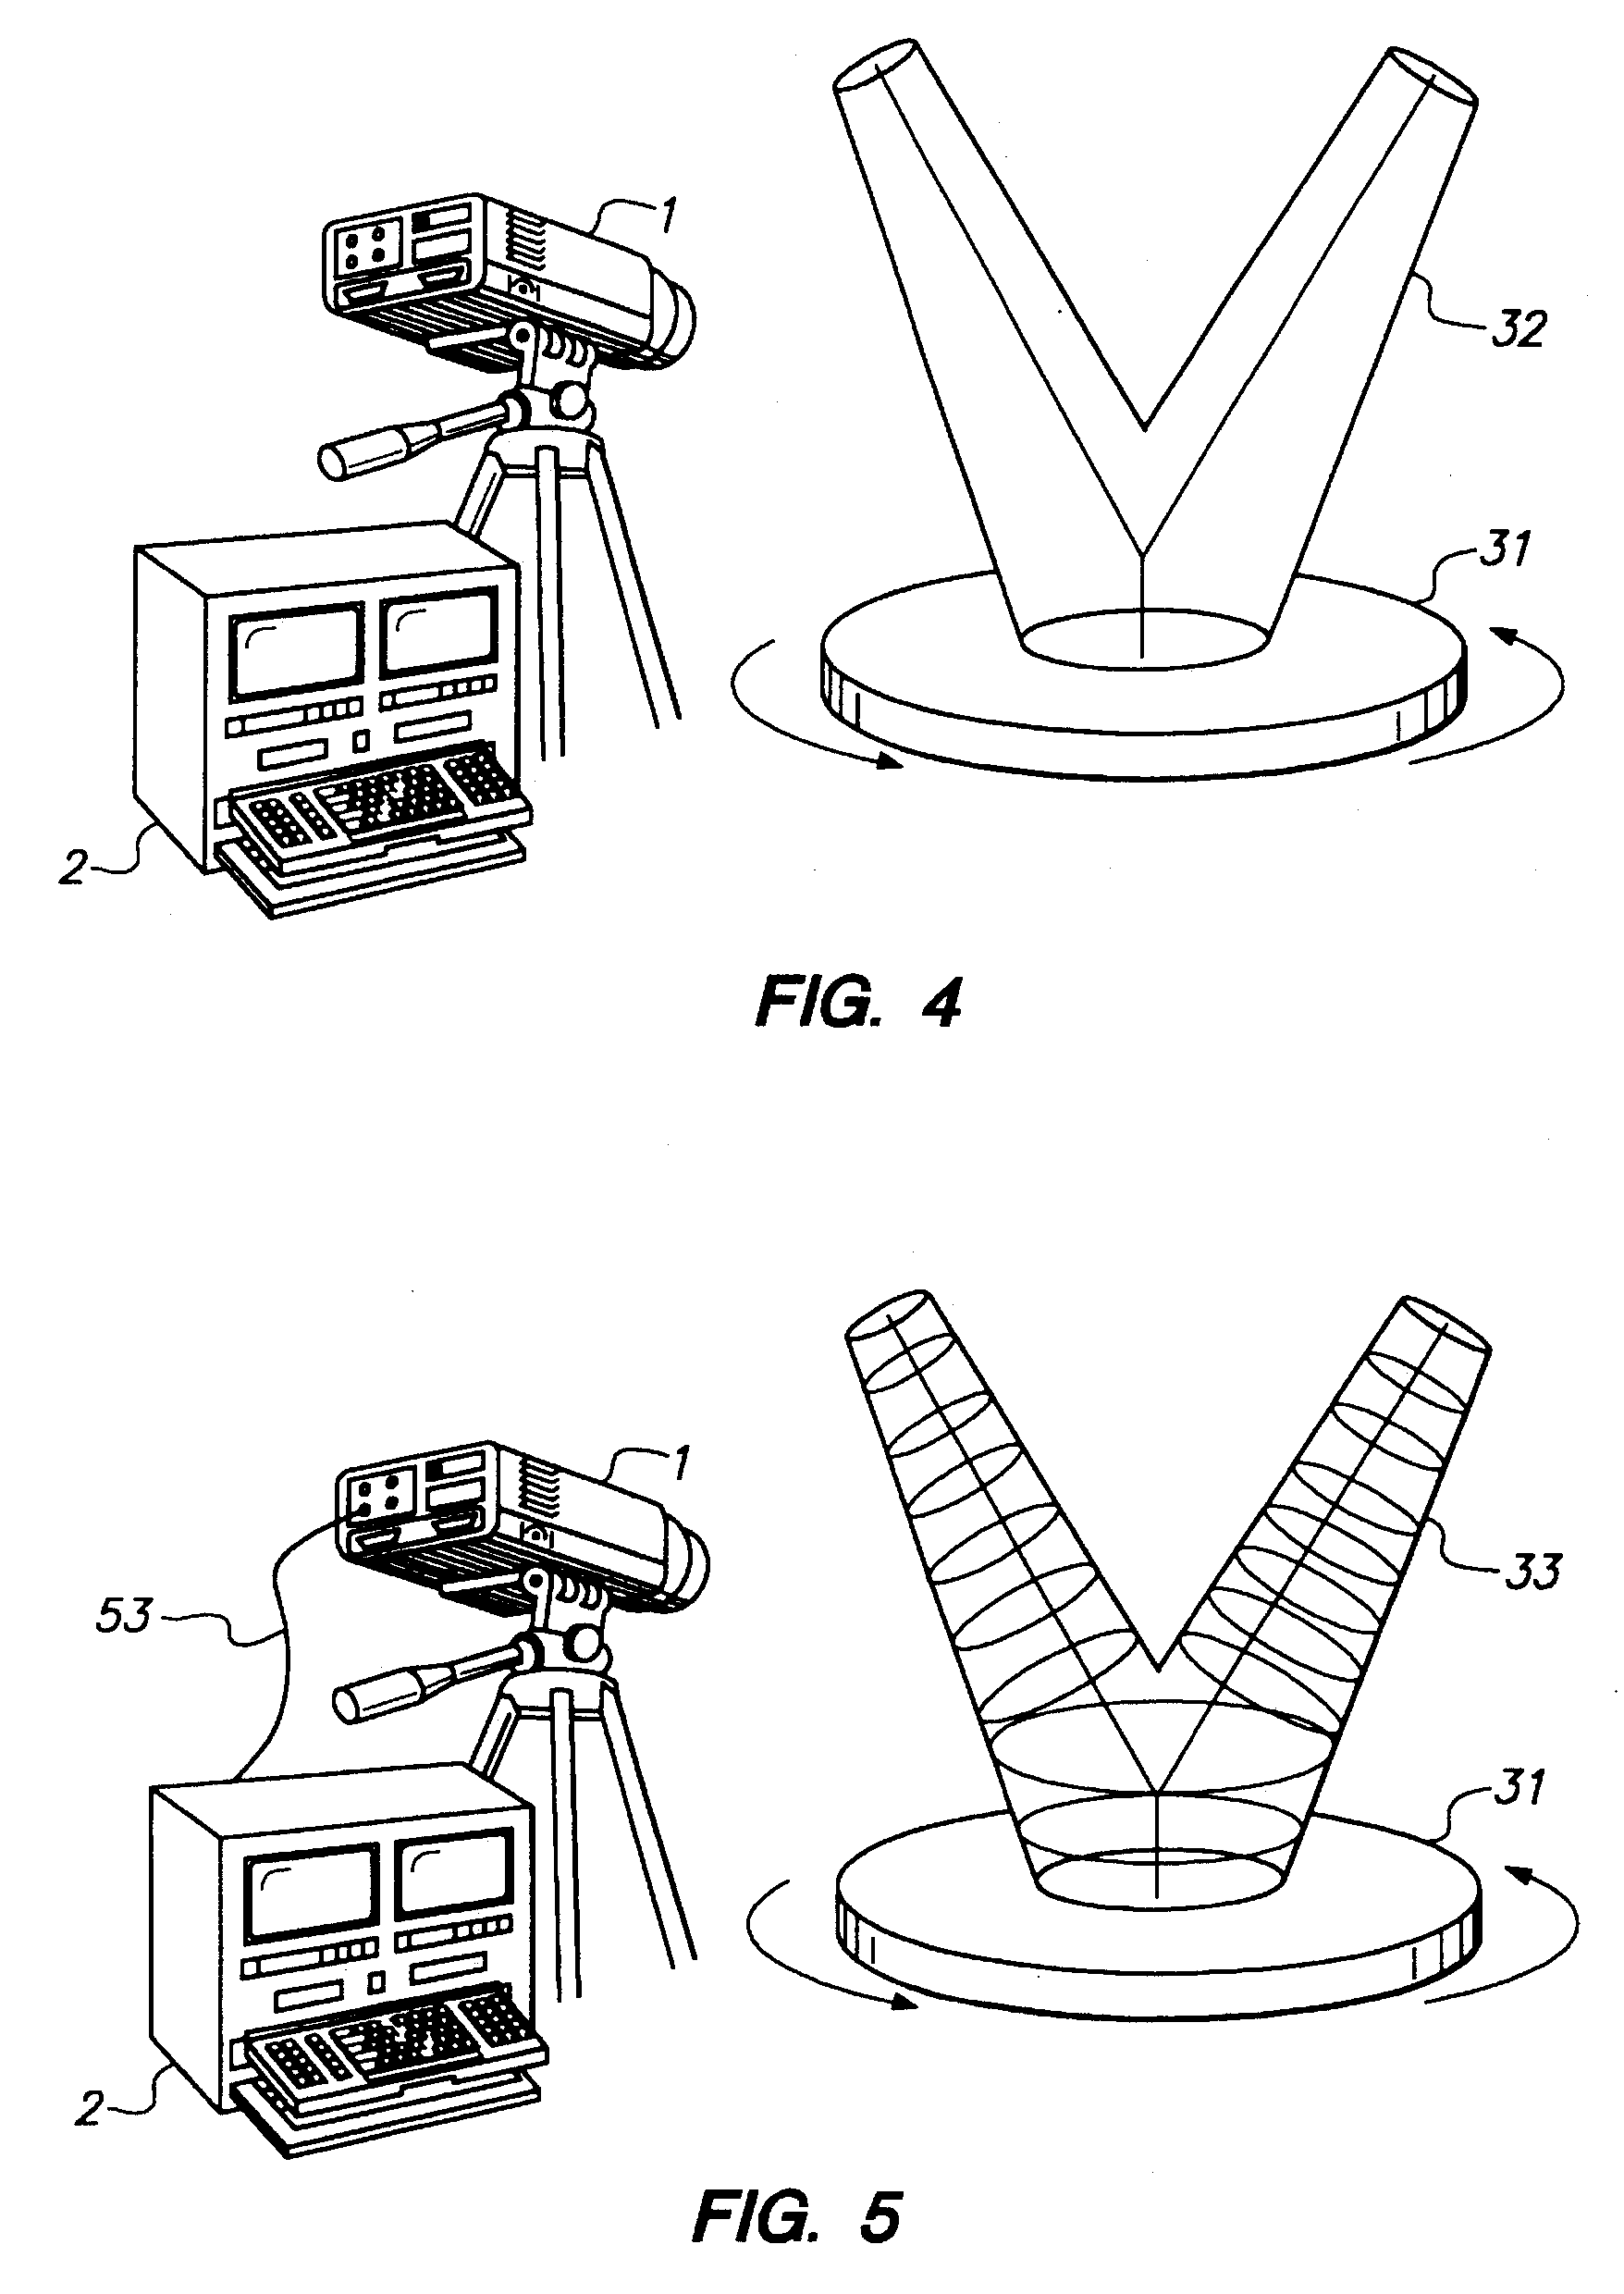
\includegraphics[width=0.3\textwidth]{img/US5530652-drawings-page-7.png}
	\caption[Sistema de captura y digitalización.]{Sistema de captura y digitalización. Fuente \cite{US5530652A}.}
	\label{fig:US5530652-7}
\end{figure}

\begin{figure}[H]
	\centering
	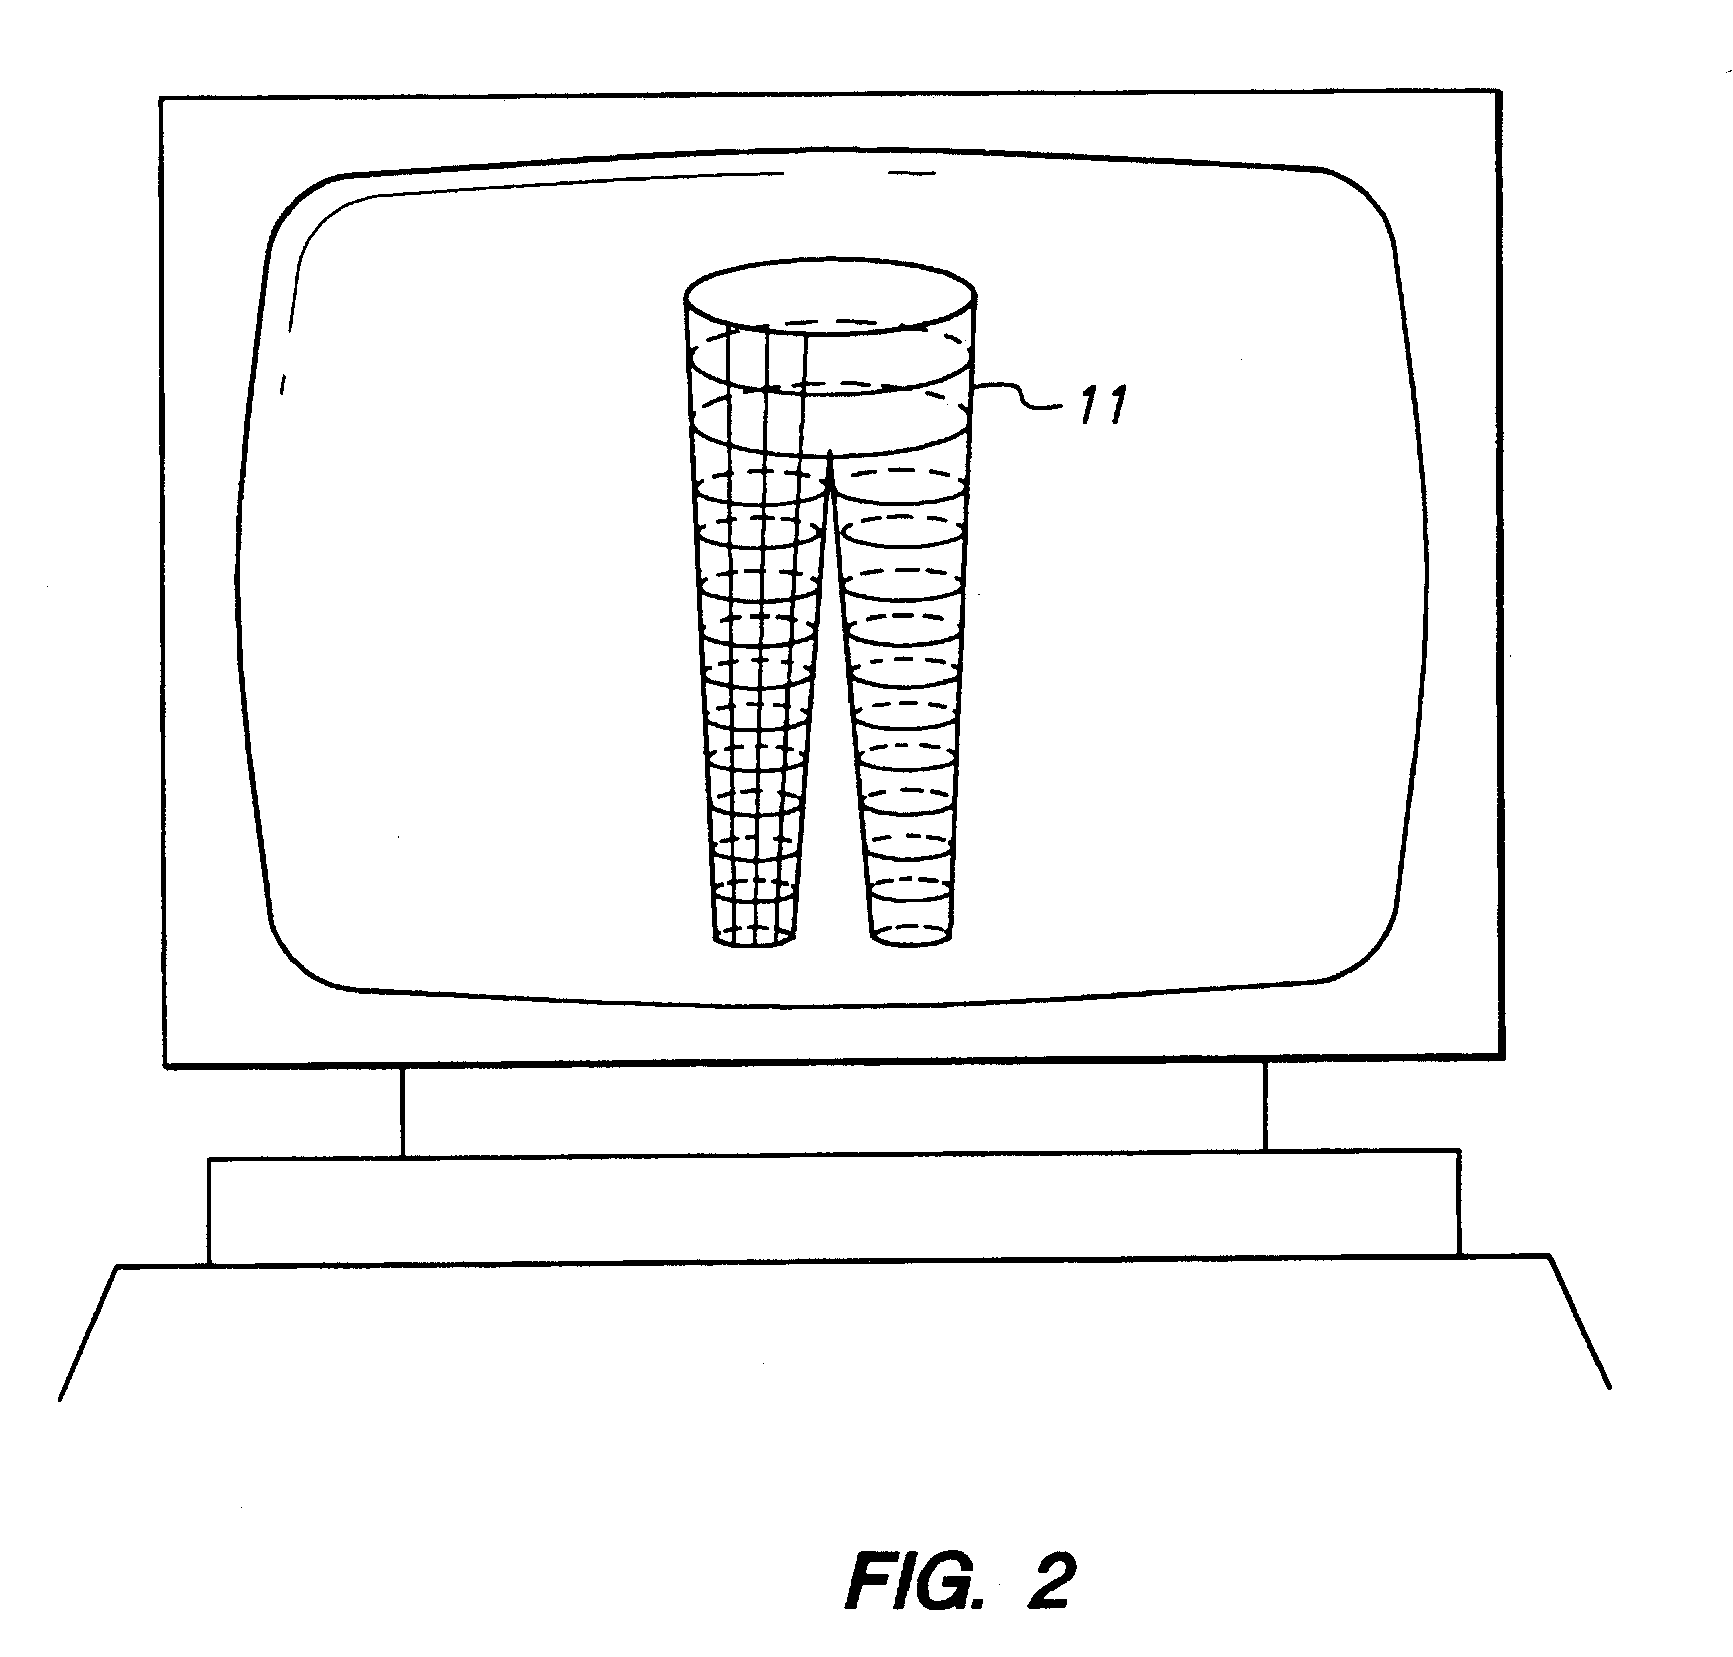
\includegraphics[width=0.4\textwidth]{img/US5530652-drawings-page-5.png}
	\caption[Digitalización de la prenda.]{Digitalización de la prenda. Fuente \cite{US5530652A}.}
	\label{fig:US5530652-5}
\end{figure}

\subsubsection{EP4095520A1}

La patente \cite{EP4095520A1} describe un sistema para el control de calidad de prendas de vestir, diseñado para identificar de manera automática y objetiva defectos tanto visibles como invisibles en la estructura interna de las prendas. Este sistema, como se observa en la Figura \ref{fig:imgf0001} se compone de dos elementos principales: un mecanismo para insuflar un gas de control a una temperatura al menos 20°C superior a la temperatura ambiente en la prenda, y un medio de captura de imágenes para detectar ubicaciones defectuosas en dicha prenda. El gas de control calentado, como aire caliente o vapor, permite detectar defectos gracias a la diferencia de temperatura que se genera en las zonas dañadas o perforadas, sin causar daño adicional a la prenda durante la inspección.

El sistema también puede incluir cámaras térmicas o de luz visible, medios para visualizar el vapor que pasa a través de la prenda y software para generar una imagen 3D de la prenda que facilita la identificación y localización precisa de los defectos. Este enfoque permite un alto grado de automatización y precisión en la detección de defectos, ofreciendo la posibilidad de determinar la naturaleza y severidad de los defectos detectados para posibles reparaciones. Además, el sistema puede ser utilizado para controlar la calidad de prendas de vestir técnicas o de alto rendimiento, asegurando que cumplan con los estándares de calidad requeridos a lo largo de su ciclo de vida, incluso después de múltiples usos y lavados.

\begin{figure}[H]
	\centering
	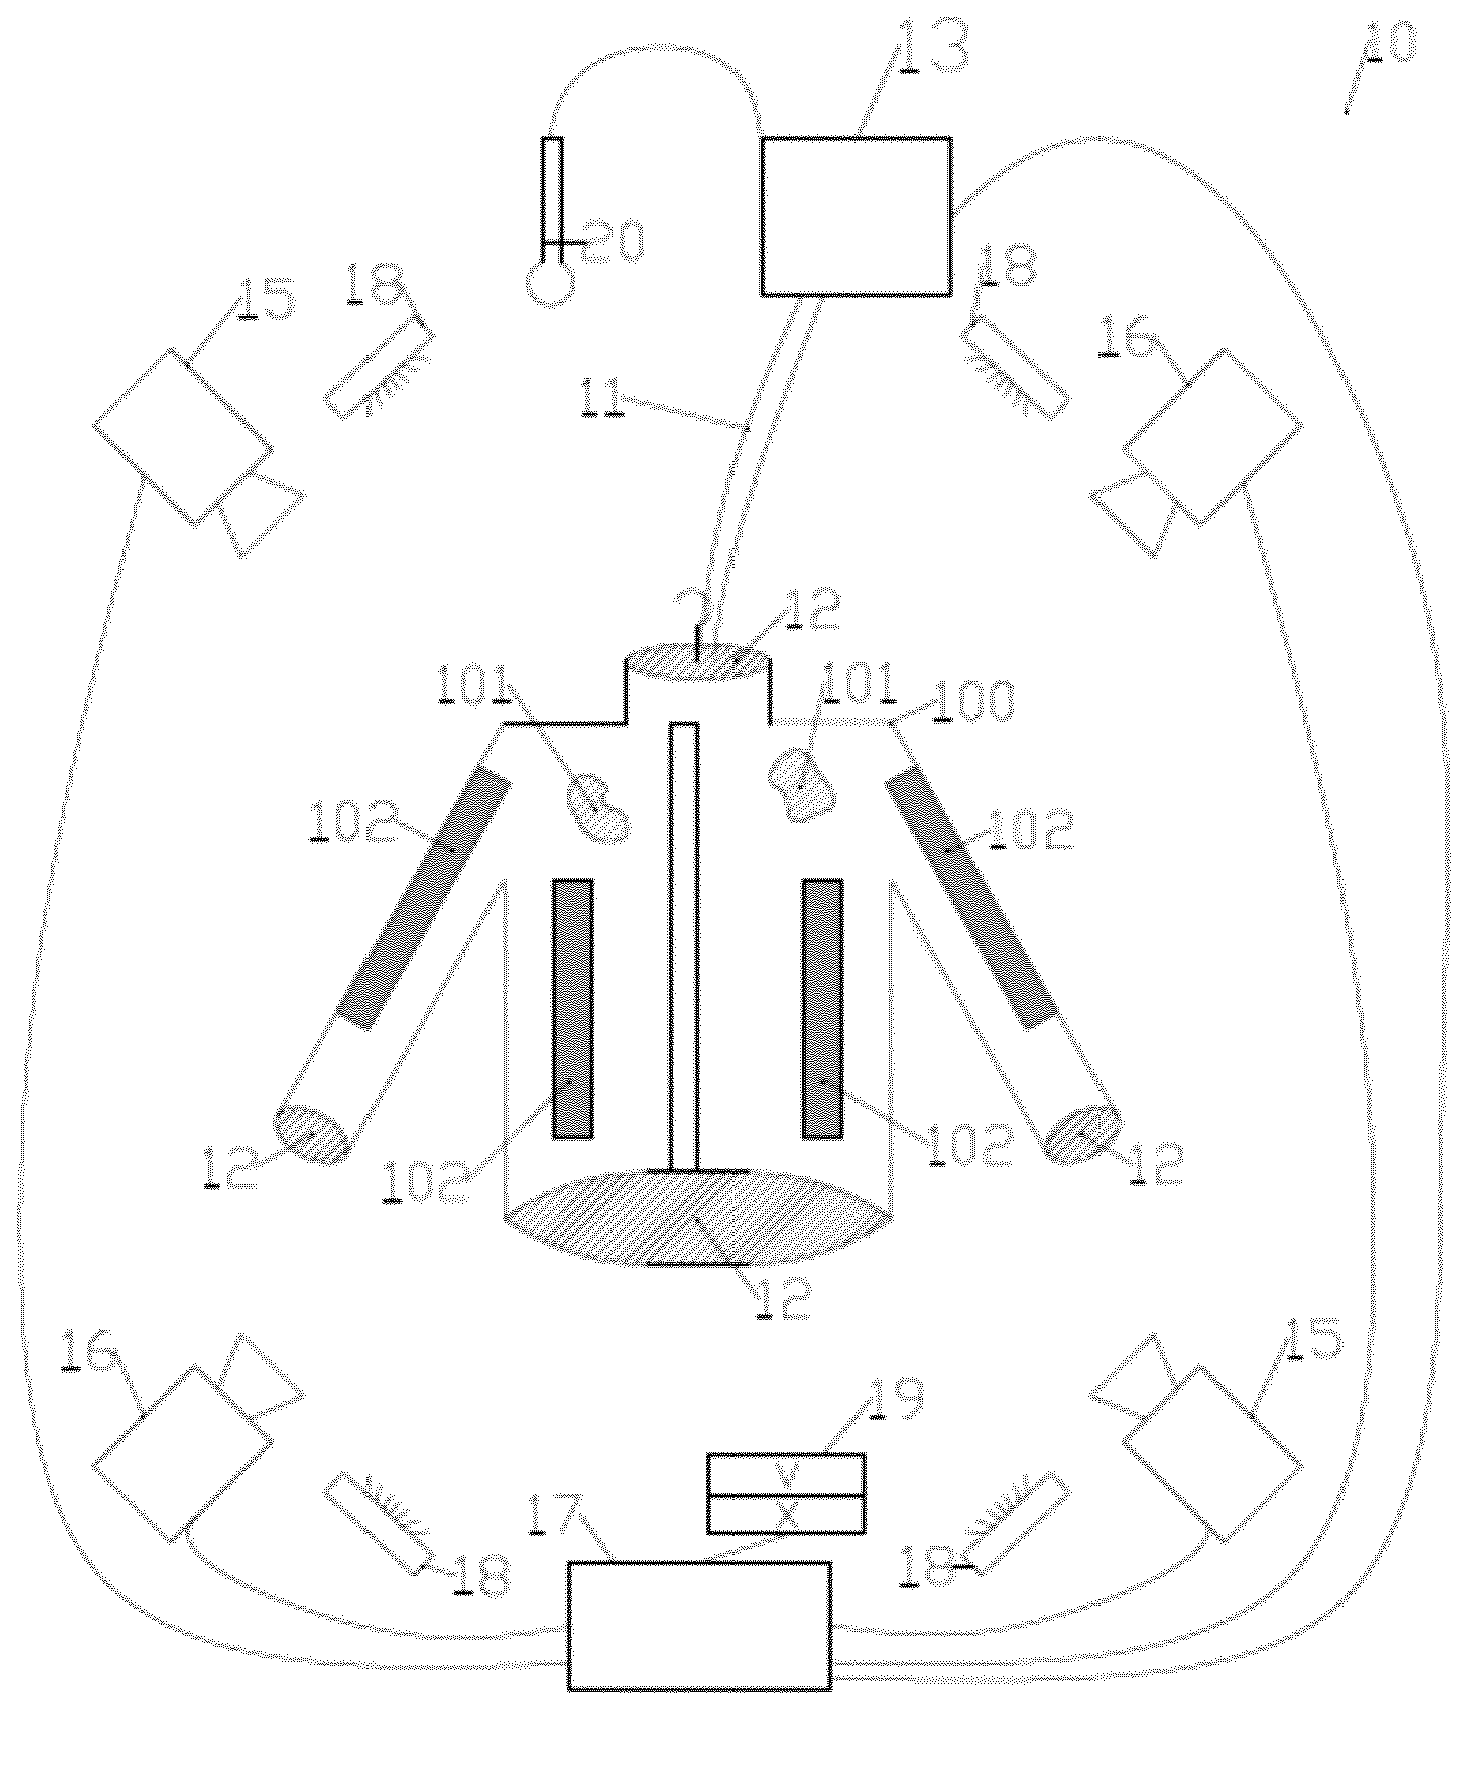
\includegraphics[width=0.4\textwidth]{img/imgf0001.png}
	\caption{Sistema de control de calidad con un mecanismo para insuflar gas.}
	\label{fig:imgf0001}
\end{figure}

\subsubsection{CN218147467U}

La patente \cite{CN218147467U} describe una máquina inteligente de detección de agujas, destinada a abordar problemas específicos en el ámbito de las máquinas de detección de agujas utilizadas para inspeccionar prendas de vestir y otros textiles en busca de partículas metálicas, como agujas rotas. El problema principal que se busca resolver es la limitación en la capacidad de procesamiento de las prendas por las máquinas de detección existentes, que puede llevar a atascos y reducir la eficiencia del proceso de inspección.

La invención se centra en un diseño de máquina de detección de agujas que incluye un escáner montado en la parte superior de un contenedor de la máquina, con mecanismos de ajuste y soporte que permiten desmontar y ajustar el escáner de manera rápida y conveniente. Este diseño permite ajustar el soporte del escáner para manejar diferentes volúmenes de prendas, facilitando la detección de agujas en prendas con variadas capacidades de procesamiento. Los elementos clave del diseño incluyen columnas y placas de soporte ajustables, resortes de soporte, y mecanismos de ajuste de altura que permiten una adaptación flexible a diferentes tamaños y cantidades de prendas.

El diseño inteligente de la máquina de detección de agujas propuesta por esta patente promete mejorar significativamente la eficiencia y flexibilidad de los procesos de inspección de metales en textiles, reduciendo el riesgo de atascos y permitiendo un ajuste rápido y fácil a diferentes necesidades de procesamiento.

\begin{figure}[H]
	\centering
	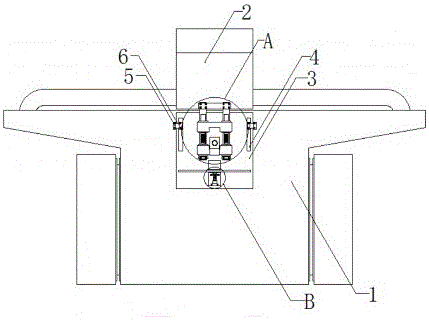
\includegraphics[width=0.6\textwidth]{img/221009135809.png}
	\caption[Detector inteligente de agujas.]{Detector inteligente de agujas. Fuente \cite{CN218147467U}.}
	\label{fig:221009135809}
\end{figure}

%CAPÍTULO 3 - DISEÑO CONCEPTUAL
% % PARA HACER QUE LA INTRODUCCIÓN NO TENGA NÚMERO
% \chapter*{Introducción}
% % PARA HACER QUE LA INTRODUCCIÓN APAREZCA EN EL ÍNDICE COMO CHAPTER
% \addcontentsline{toc}{chapter}{Introducción}

% \chapter{Marco Teórico}
% \section{Visión Artificial}
% \subsection{YOLOv8}
% \section{Control de calidad en prendas de vestir}
% \subsection{NTP-ISO 8559-2:2020}

\chapter{Diseño Conceptual}

En este capítulo se presentan alternativas de conceptos solución, los cuales son propuestos en función de la lista de requerimientos, el diagrama de funciones y la matriz morfológica. Luego, los diseños de concepto solución son calificados por una evaluación técnica-económica; con lo cual se obtiene el concepto de solución óptimo.

\section{Lista de exigencias}

Sobre la base de los parámetros necesarios del sistema, los cuales fueron identificados en el Estado del Arte visto en el Capítulo \ref{Estado del Arte}, se elaboró la lista de exigencias mostrada en la Tabla \ref{tab:lista_exigencias}. Esta resume los requerimientos básicos para el diseño del sistema propuesto.

\begin{longtable}{|c|p{4.5em}|p{22.5em}|p{6em}|}
	\caption[Lista de Requerimientos.]{Lista de Requerimientos. Fuente: Elaboración propia.}\label{tab:lista_exigencias}\\
	\hline
	\multicolumn{4}{|p{37.5em}|}{\textbf{LISTA DE EXIGENCIAS}} \bigstrut\\
	\hline
	\multicolumn{2}{|p{9em}|}{\textbf{PROYECTO}} & DISEÑO DE UN SISTEMA PARA EL CONTROL DE CALIDAD DE PRENDAS DE VESTIR UTILIZANDO VISIÓN ARTIFICIAL & Fecha: 06/03/24 \bigstrut\\
	\hline
	\multicolumn{2}{|p{9em}|}{\textbf{CLIENTE}} & Pontificia Universidad Católica del Perú & Elaborado por: A. Luna \bigstrut\\
	\hline
	\multicolumn{2}{|p{9em}|}{\parbox{4cm}{\textbf{FUNCIÓN} \\ \textbf{PRINCIPAL}}
	} & \multicolumn{2}{p{28.5em}|}{Detectar y controlar la calidad de prendas de vestir, identificando tanto los defectos visuales como los relacionados con las medidas.} \bigstrut\\
	\hline
	\endfirsthead \caption* {Tabla \ref{tab:lista_exigencias}: Lista de Requerimientos (Continuación).}\\
	\hline
	\multicolumn{1}{|p{4.5em}|}{\textbf{Fecha}} & \textbf{Deseo o Exigencia} & \textbf{Descripción} & \textbf{Responsable} \bigstrut\\
	\hline
	\endhead
	\multicolumn{4}{|p{37.5em}|}{\textbf{FUNCIONES}} \bigstrut\\
	\hline
	6/03/2024 & E     & La prenda ingresará de manera estirada y sin arrugas. & A. Luna \bigstrut\\
	\hline
	6/03/2024 & E     & Se debe detectar las manchas, hilos salidos y agujeros presentes en las prendas. & A. Luna \bigstrut\\
	\hline
	6/03/2024 & E     & Se debe detectar metales presentes que se hayan dejado en las prendas como agujas o alfileres. & A. Luna \bigstrut\\
	\hline
	\multicolumn{4}{|p{37.5em}|}{\textbf{OPERACIÓN}} \bigstrut\\
	\hline
	6/03/2024 & D     & El prototipo deberá poder controlar la calidad de como mínimo 30 prendas/hora. & A. Luna \bigstrut\\
	\hline
	\multicolumn{4}{|p{37.5em}|}{\textbf{ALIMENTACIÓN}} \bigstrut\\
	\hline
	6/03/2024 & E     & Eléctrica, 220V (Monofásica). & A. Luna \bigstrut\\
	\hline
	\multicolumn{4}{|p{37.5em}|}{\textbf{SOFTWARE}} \bigstrut\\
	\hline
	6/03/2024 & D     & Se debe emplear un software, algoritmo o modelo de código abierto para la implementación de la funcionalidad de la visión por computadora. & A. Luna \bigstrut\\
	\hline
	6/03/2024 & E     & El prototipo debe disponer de una GUI para la interacción con los operarios del sistema.  & A. Luna \bigstrut\\
	\hline
	\multicolumn{4}{|p{37.5em}|}{\textbf{SEÑALES}} \bigstrut\\
	\hline
	6/03/2024 & E     & Entrada: Encendido, apagado, inicio de proceso, fin de proceso.\newline{}Salida: Luz piloto de alimentación, encendido y funcionamiento. & A. Luna \bigstrut\\
	\hline
	\multicolumn{4}{|p{37.5em}|}{\textbf{INTERFAZ}} \bigstrut\\
	\hline
	6/03/2024 & E     & Tablero de control con:\newline{}- Llave de encendido general\newline{}- Pulsador de inicio y parada de proceso\newline{}- Parada de emergencia manual\newline{}- Indicadores luminosos de alimentación,funcionamiento encendido & A. Luna \bigstrut\\
	\hline
	\multicolumn{4}{|p{37.5em}|}{\textbf{CONDICIONES DE OPERACIÓN}} \bigstrut\\
	\hline
	6/03/2024 & E     & Ambiente de trabajo con humedad relativa máxima de 85\%, a 100 msmn (condiciones de la costa peruana, en un laboratorio de pruebas). & A. Luna \bigstrut\\
	\hline
	6/03/2024 & D     & Ambiente de trabajo industrial, con máquinas contiguas trabajando en paralelo. & A. Luna \bigstrut\\
	\hline
	\multicolumn{4}{|p{37.5em}|}{\textbf{CONTROL}} \bigstrut\\
	\hline
	6/03/2024 & E     & Alimentación de ropa manual hecha por un operario. & A. Luna \bigstrut\\
	\hline
	6/03/2024 & E     & Detección de defectos automática. & A. Luna \bigstrut\\
	\hline
	6/03/2024 & E     & Detección de medidas automática. & A. Luna \bigstrut\\
	\hline
	6/03/2024 & D     & Regulación de velocidad de procesamiento de prendas. & A. Luna \bigstrut\\
	\hline
	6/03/2024 & E     & Sensores grado mínimo IP 63 (resistencia al polvo y humedad condensada). & A. Luna \bigstrut\\
	\hline
	6/03/2024 & E     & Parada de emergencia automática en caso de atasco o sobrecarga. & A. Luna \bigstrut\\
	\hline
	\multicolumn{4}{|p{37.5em}|}{\textbf{SEGURIDAD}} \bigstrut\\
	\hline
	6/03/2024 & E     & El tablero de control debe contar con protección contra polvo y liquido grado IP64. & A. Luna \bigstrut\\
	\hline
	\multicolumn{4}{|p{37.5em}|}{\textbf{CONTROL DE CALIDAD}} \bigstrut\\
	\hline
	6/03/2024 & E     & La detección de defectos debe tener una efectividad del 90\%. & A. Luna \bigstrut\\
	\hline
	6/03/2024 & E     & La detección de las medidas de la prenda debe tener una presición del 90\%. & A. Luna \bigstrut\\
	\hline
	\multicolumn{4}{|p{37.5em}|}{\textbf{MONTAJE}} \bigstrut\\
	\hline
	6/03/2024 & D     & El sistema presenta la posibilidad de acoplar varias lineas en paralelo para incrementar la productividad. & A. Luna \bigstrut\\
	\hline
	\multicolumn{4}{|p{37.5em}|}{\textbf{MATERIAL}} \bigstrut\\
	\hline
	6/03/2024 & E     & Materiales que eviten la acumulaciónd de manchas y polvo. & A. Luna \bigstrut\\
	\hline
	\multicolumn{4}{|p{37.5em}|}{\textbf{FABRICACIÓN}} \bigstrut\\
	\hline
	6/03/2024 & E     & El diseño debe contar con componentes estandarizados que esten disponibles en el mercado local. & A. Luna \bigstrut\\
	\hline
	6/03/2024 & D     & Los elementos diseñados deben evitar el mantenimiento complejo. & A. Luna \bigstrut\\
	\hline
	\multicolumn{4}{|p{37.5em}|}{\textbf{MANTENIMIENTO}} \bigstrut\\
	\hline
	6/03/2024 & E     & Los elementos motrices serán accesibles y las superficies fáciles de limpiar. Los componentes electrónicos no deben estar expuestas al polvo. & A. Luna \bigstrut\\
	\hline
	\multicolumn{4}{|p{37.5em}|}{\textbf{DIMENSIONES}} \bigstrut\\
	\hline
	6/03/2024 & E     & El prototipo no deberá ocupar un volumen mayor a 3m x 3m x 3m para poder ser construido en un laboratorio. & A. Luna \bigstrut\\
	\hline
	6/03/2024 & E     & El prototipo no deberá pesar más de 30kg para poder ser movilizado por una persona. & A. Luna \bigstrut\\
	\hline
	\multicolumn{4}{|p{37.5em}|}{\textbf{COSTO}} \bigstrut\\
	\hline
	6/03/2024 & D     & Fabricación: 30000 soles (A nivel de prototipo). & A. Luna \bigstrut\\
	\hline
\end{longtable}%


\section{Estructura de funciones}

La estructura de funciones se utiliza para describir el seguimiento de las señales de entrada y salida dentro del sistema, detallando así la interacción entre las funciones internas de cada dominio. En la subsección \ref{Black Box}, se introducirá el \textit{Black Box}, en el cual se expondrán todas las entradas y salidas pertinentes al sistema. Por otro lado, en la subsección \ref{Funciones Parciales}, se elaborará sobre todas las funciones correspondientes a los subsistemas que integran el sistema en su totalidad, así como las conexiones existentes entre cada una de estas funciones.

\subsection{Black Box}
\label{Black Box}

El diseño de caja negra que se presenta en la Figura \ref{fig:BLACK_BOX} se detallan las entradas y salidas del sistema. La entrada principal del sistema es una prenda de vestir. Para funcionar, este sistema se alimenta de energía a través de una fuente eléctrica estándar de 220VAC monofásica, proporcionando así electricidad a los dominios de transporte, electrónico y de software involucrados. El sistema también está equipado con señales de entrada para su control, incluyendo comandos de inicio, detención y parada de emergencia, tanto en formatos físicos como virtuales. Debido a la ineficiencia de los componentes mecánicos y electrónicos se muestra como salida la energía residual en forma de calor.

\begin{figure}[H]
	\centering
	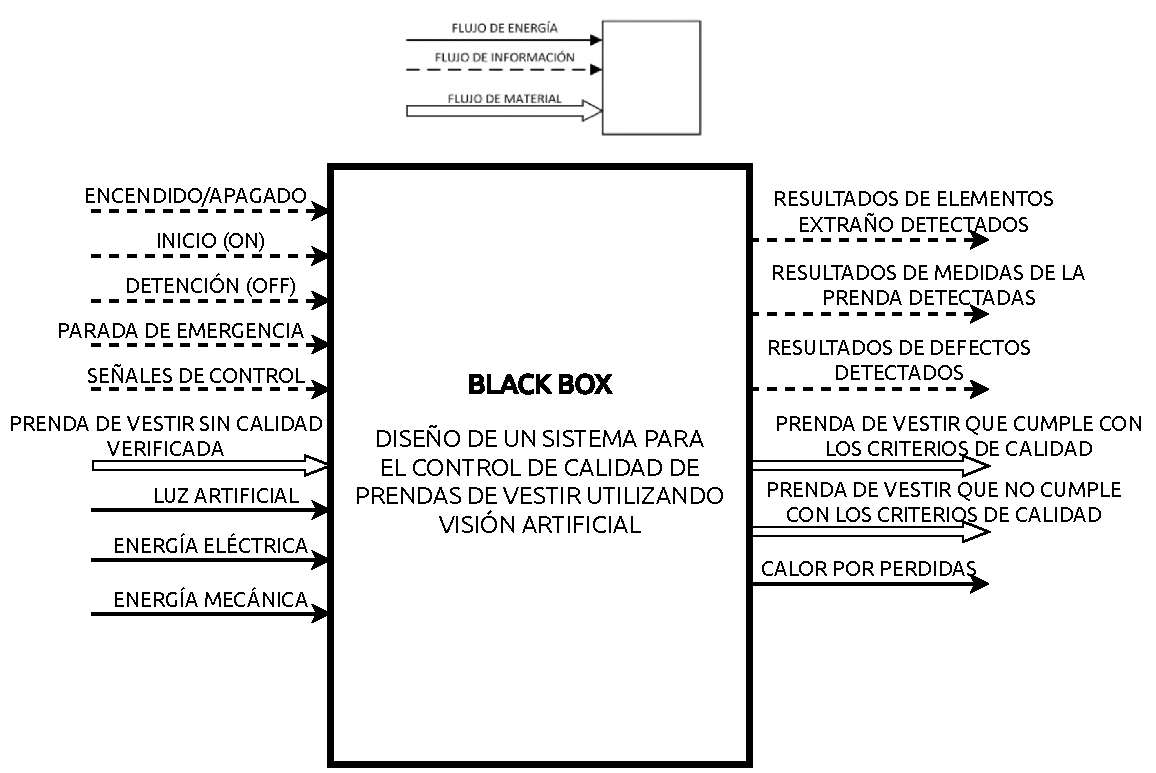
\includegraphics[width=\textwidth]{img/BLACK_BOX.drawio.pdf}
	\caption[Black Box.]{Black Box. Fuente: Elaboración propia.}
	\label{fig:BLACK_BOX}
\end{figure}

\subsection{Funciones Parciales}
\label{Funciones Parciales}

Aquellos procesos que interactúan directamente con el material a ser analizado conforman las funciones básicas del sistema. Estas funciones se muestran en la Figura \ref{fig:ESTRUCTURA_DE_FUNCIONES}. Primero, prendas de vestir sin clasificar son ingresadas por un operario para iniciar el proceso de detección de defectos. Se debe contar además con algún método que maximice la superficie de la prenda que pueda ser visible para la cámara, con el fin de incrementar la efectividad del proceso de detección y clasificación según los criterios de selección. Luego esta prenda es analizada mediante módulos especializados en la detección de defectos visuales y otro módulo encargado de identificar la presencia de elementos metálicos extraños. Como resultado de este proceso, se producirá una imagen que resalta los defectos detectados en la prenda donde se señala la existencia o no de elementos metálicos ajenos. Finalmente, las prendas ya verificadas serán transportadas a la disposición final adecuada.

\begin{sidewaysfigure}
	\begin{figure}[H]
		\centering
		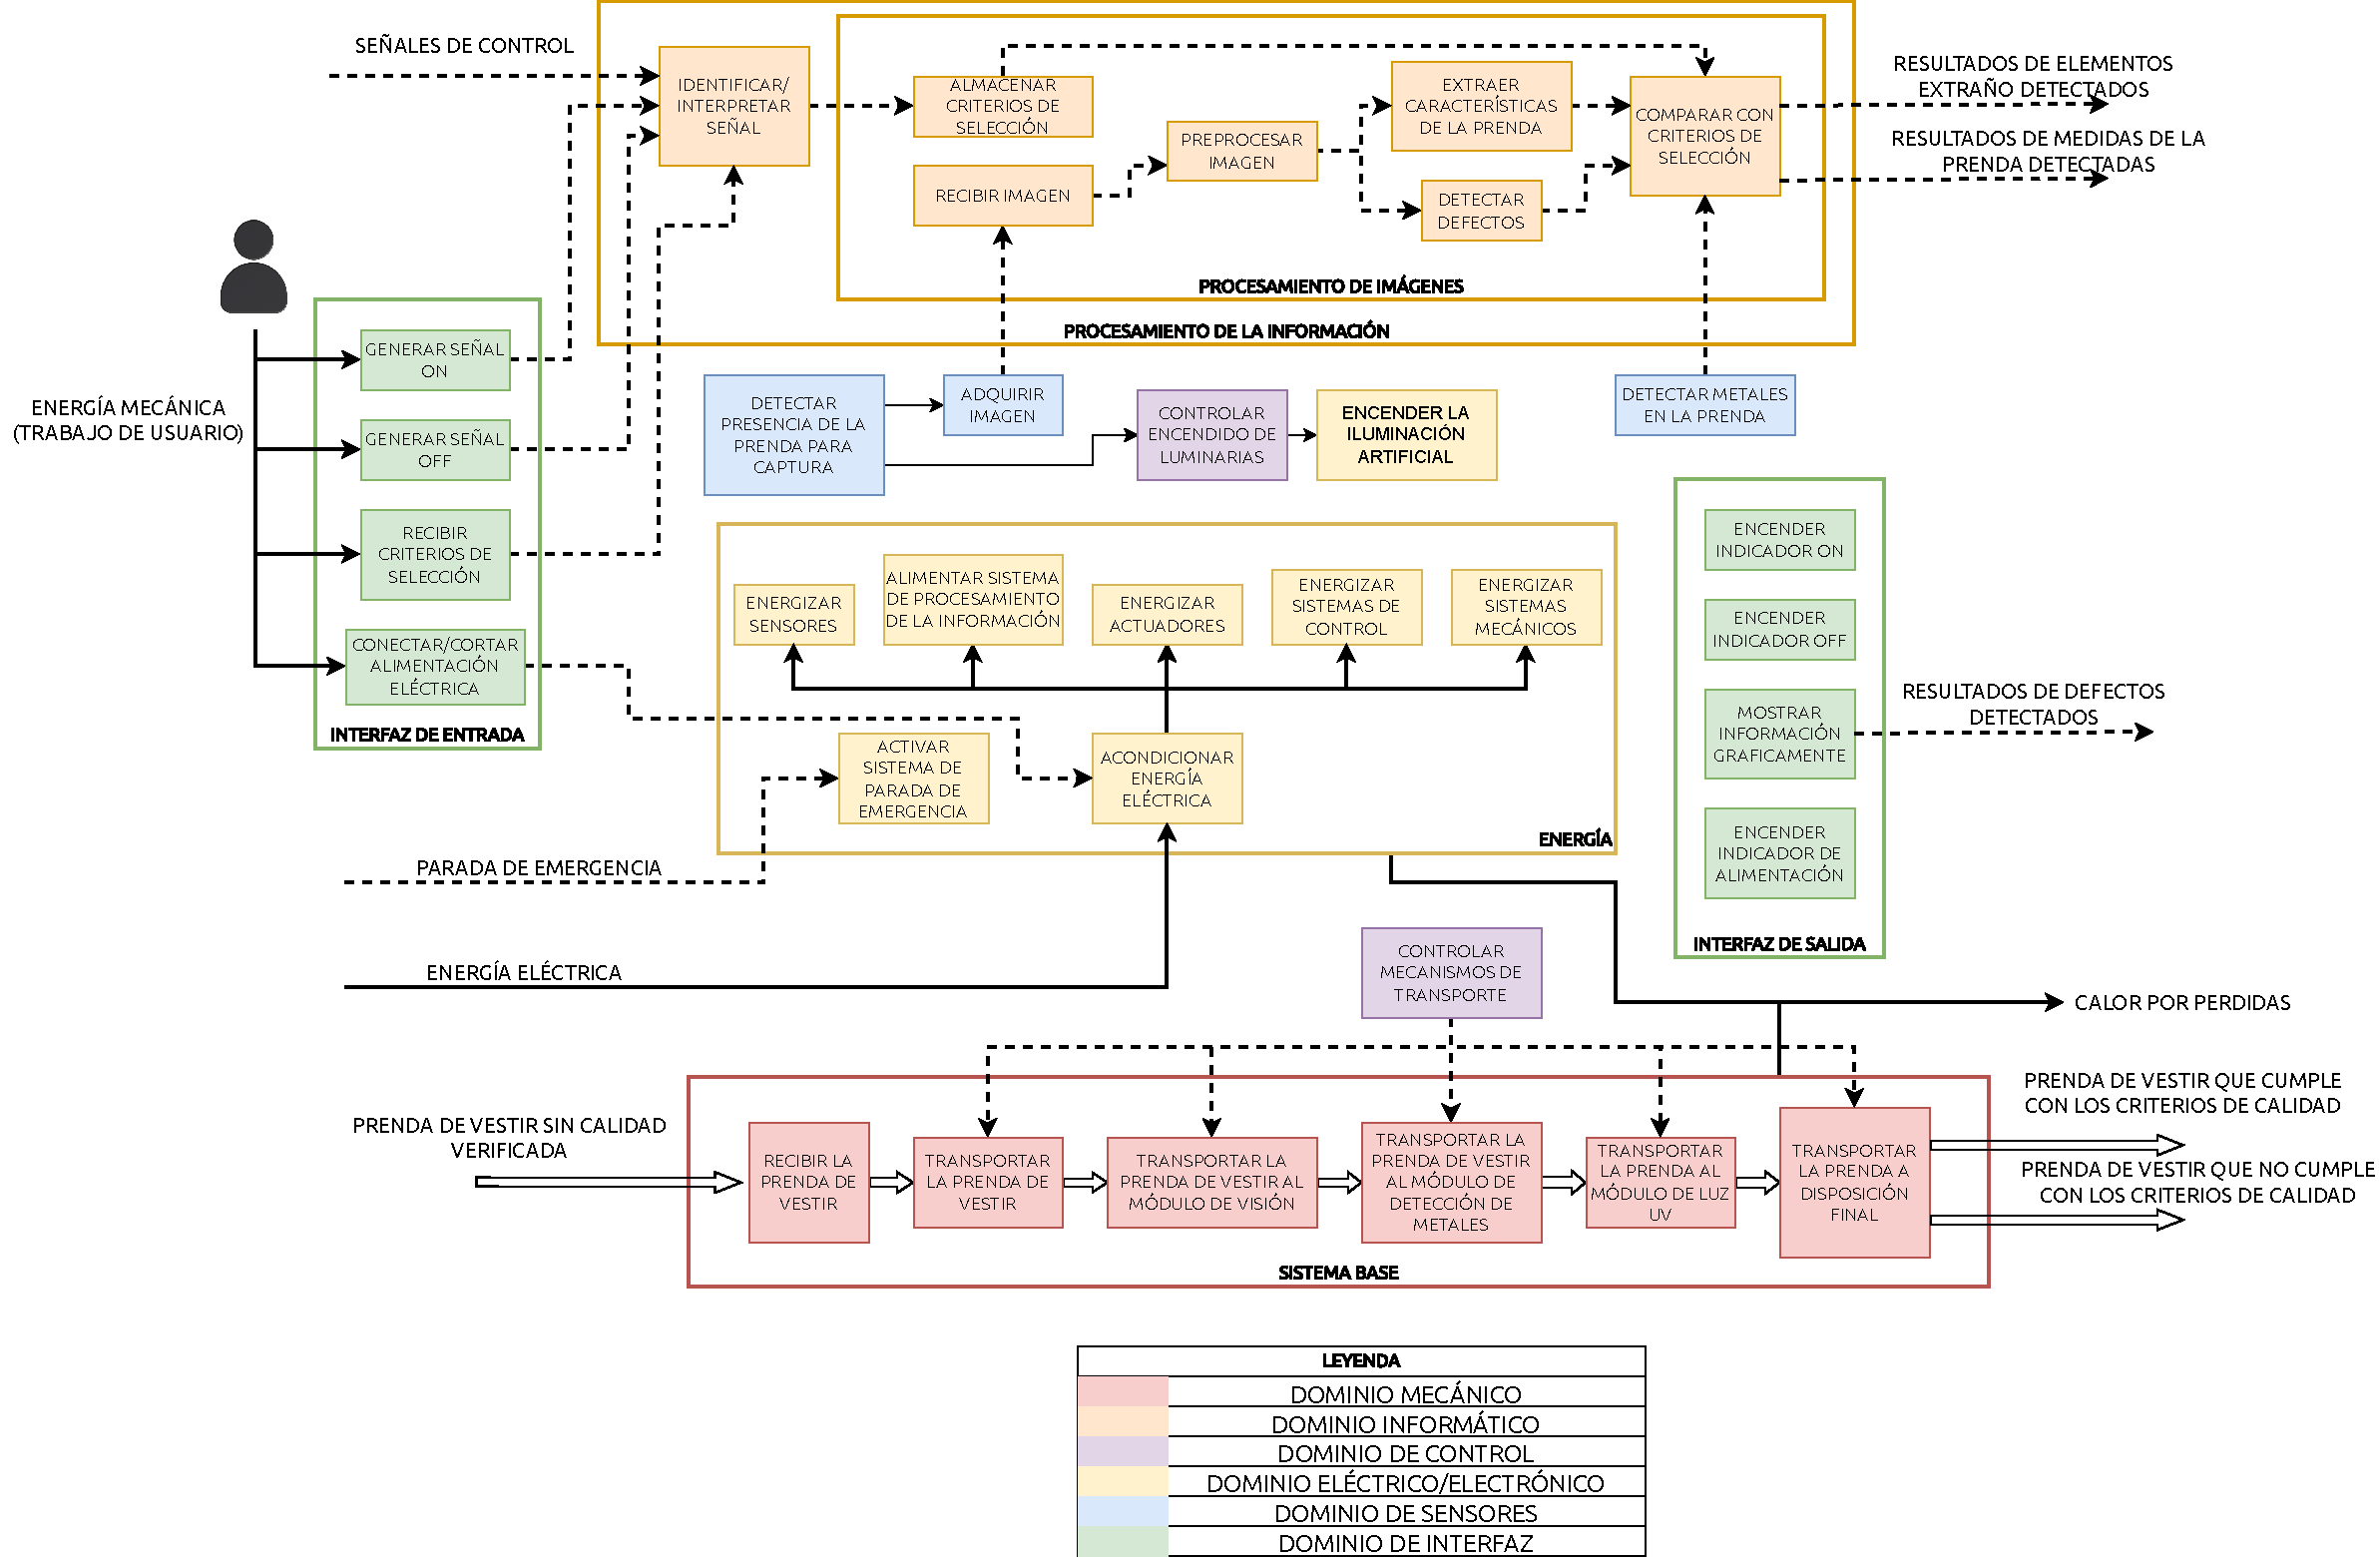
\includegraphics[width=\textwidth]{img/ESTRUCTURA_DE_FUNCIONES.drawio.pdf}
		\label{fig:ESTRUCTURA_DE_FUNCIONES}
		\caption[Estructura de funciones del sistema.]{Estructura de funciones del sistema. Fuente: Elaboración propia.}
	\end{figure}
\end{sidewaysfigure}

\subsubsection{Dominio Mecánico}

El dominio mecánico abarca todas las operaciones físicas y movimientos asociados con el manejo de prendas de vestir, como se muestra en la Figura \ref{fig:EF_DM}. Incluye la recepción de las prendas, su transporte a través de diferentes estaciones de procesamiento como módulos de visión artificial y detección de metales. Este dominio garantiza que las prendas se muevan eficientemente de una etapa a otra, facilitando su análisis y clasificación según cumplan o no con los criterios de calidad establecidos.

\begin{figure}[h]
	\centering
	
\includegraphics[width=\textwidth]{img/EF_DM.pdf}
	\caption[Estructura de funciones del dominio mecánico.]{Estructura de funciones del dominio mecánico. Fuente: Elaboración propia.}
	\label{fig:EF_DM}
\end{figure}

\subsubsection{Dominio Informático}

El dominio informático se centra en el procesamiento de la información obtenida de las prendas , como se muestra en la Figura \ref{fig:EF_DIn}. Este dominio comprende la adquisición y preprocesamiento de imágenes de las prendas, extracción de características relevantes, detección de defectos, y comparación de estos datos con criterios de selección predefinidos para determinar la calidad de las prendas. Este dominio es crucial para interpretar los datos capturados y tomar decisiones basadas en la información procesada.

\begin{figure}[h]
	\centering
	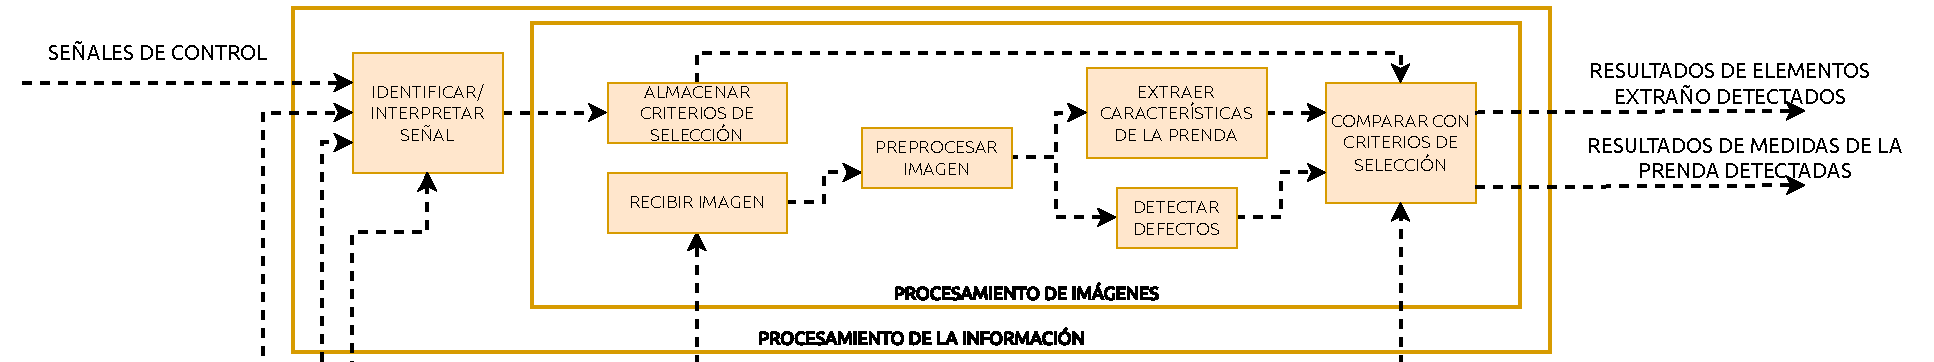
\includegraphics[width=\textwidth]{img/EF_DIn.pdf}
	\caption[Estructura de funciones del dominio informático.]{Estructura de funciones del dominio informático. Fuente: Elaboración propia.}
	\label{fig:EF_DIn}
\end{figure}

\subsubsection{Dominio de Control}

El dominio de control, mostrado en la Figura \ref{fig:EF_DC}, incluye la lógica de control y los mecanismos de decisión que guían las operaciones del sistema. Esto implica generar señales de encendido/apagado basadas en la información procesada, manejar interfaces de entrada/salida, y activar mecanismos de parada de emergencia. Este dominio es esencial para coordinar las actividades de los otros dominios y asegurar que el sistema responda adecuadamente a las condiciones de operación y a los requisitos de procesamiento.

\begin{figure}[h]
	\centering
	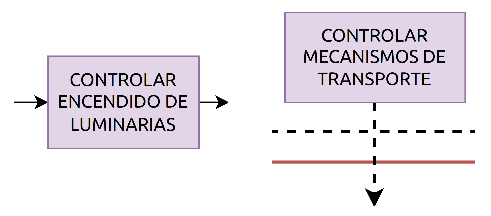
\includegraphics[width=0.4\textwidth]{img/EF_DC.pdf}
	\caption[Estructura de funciones del dominio de control.]{Estructura de funciones del dominio de control. Fuente: Elaboración propia.}
	\label{fig:EF_DC}
\end{figure}

\subsubsection{Dominio Eléctrico/Electrónico}

Este dominio se ocupa de la alimentación y control eléctrico de todos los componentes del sistema, tal y como se muestra en la Figura \ref{fig:EF_DEE}. Desde energizar los sensores hasta alimentar los sistemas de procesamiento de información, actuadores, y sistemas de control, este dominio asegura que todos los elementos electrónicos del sistema reciban la energía necesaria para su funcionamiento. Además, gestiona la iluminación necesaria para la adquisición de imágenes y la señalización a través de indicadores ON/OFF.

\begin{figure}[h]
	\centering
	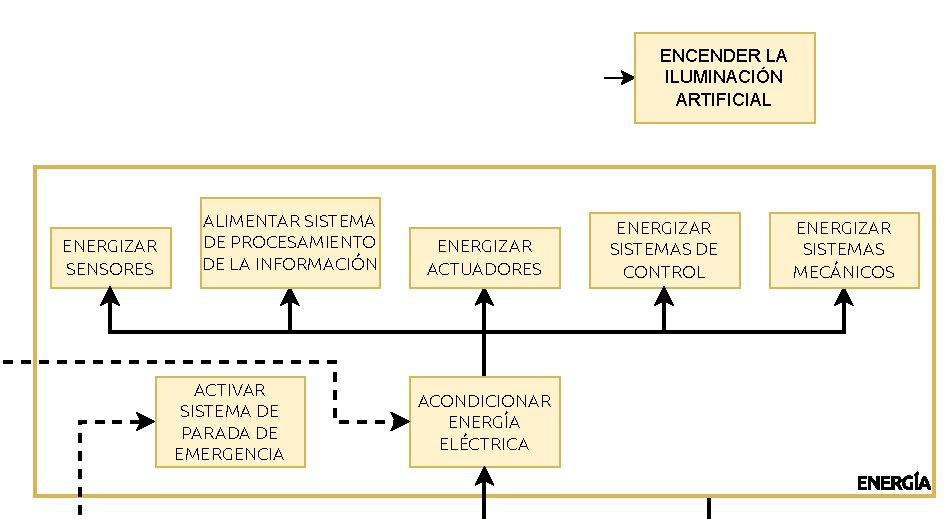
\includegraphics[width=0.8\textwidth]{img/EF_DEE.pdf}
	\caption[Estructura de funciones del dominio eléctrico/electrónico.]{Estructura de funciones del dominio eléctrico/electrónico. Fuente: Elaboración propia.}
	\label{fig:EF_DEE}
\end{figure}

\subsubsection{Dominio de Sensores}

Este dominio comprende la detección y recopilación de datos a través de sensores diseñados para identificar características específicas de las prendas. Esto se muestra en la Figura \ref{fig:EF_DS}. Se identifica la presencia de metales o la preparación para la captura de imágenes. La información recogida por los sensores es vital para el adecuado funcionamiento del sistema, ya que permite adaptar las operaciones a las condiciones actuales y a las necesidades específicas de procesamiento de las prendas.

\begin{figure}[h]
	\centering
	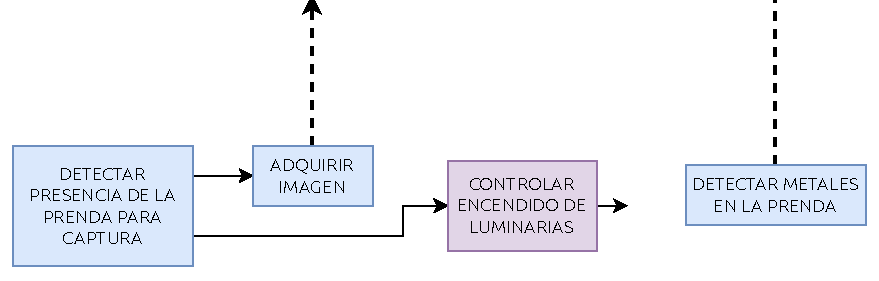
\includegraphics[width=0.7\textwidth]{img/EF_DS.pdf}
	\caption[Estructura de funciones del dominio de sensores.]{Estructura de funciones del dominio de sensores. Fuente: Elaboración propia.}
	\label{fig:EF_DS}
\end{figure}

\subsubsection{Dominio de Interfaz}

El dominio de interfaz esta dedica en interactuar con los usuarios finales del sistema. Como se muestra en la Figura \ref{fig:EF_DI}, a través del empleo de la energía mecánica del operario del sistema para generar las señales de control, lo cual incluye la señal de encendido, apagado o de parada de emergencia. Por otro lado, La información de los resultados de todos los procesos realizados por el sistema se mostraran mediante una interfaz que las muestre de manera ordenada y concisa.

\begin{figure}[h]
	\centering
	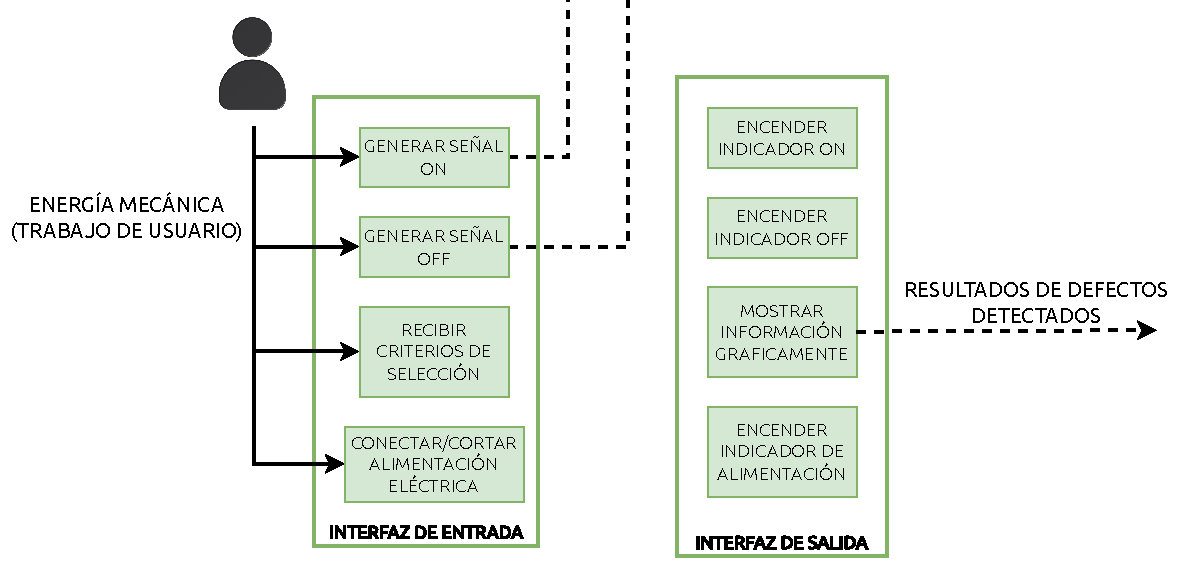
\includegraphics[width=\textwidth]{img/EF_DI.pdf}
	\caption[Estructura de funciones del dominio de interfaz.]{Estructura de funciones del dominio de interfaz. Fuente: Elaboración propia.}
	\label{fig:EF_DI}
\end{figure}

\section{Matriz morfológica}

A continuación, se presentan las diferentes matrices morfológicas para cada dominio previamente descrito, esta metodología ayudó a visualizar las diferentes opciones y escoger una solución idónea para los requerimientos. En las Tablas \ref{tab:MM_DI}, \ref{tab:MM_DM}, \ref{tab:MM_DIn}, \ref{tab:MM_DC}, \ref{tab:MM_DEE} y \ref{tab:MM_DS} se observan las matrices morfológicas del dominio de interfaz, dominio mecánico, dominio informático, dominio de control, dominio eléctrico/electrónico y dominio de sensores respectivamente. 
Las cuatro alternativas de solución se clasificarán siguiendo la leyenda de colores mostrada en la Tabla \ref{tab:leyenda_colores_soluciones}. Estos soluciones se generan al colocar un $\B{\blacklozenge}{1.35}$ con el color correspondiente al concepto de solución para cada función parcial de las matrices morfológicas.

\begin{table}[H]
	\centering
	\caption[Leyenda de colores para los conceptos de solución en las matriz morfológica.]{Leyenda de colores para los conceptos de solución en las matriz morfológica. Fuente: Elaboración propia.}
	\begin{tabular}{|c|c|c|}
		\hline
		\textbf{Soluciones} & \textbf{Tipo de Solución} & \textbf{Color} \bigstrut\\
		\hline
		Solución 1 & Accesible & \cellcolor[rgb]{ 1,  0,  0} \bigstrut\\
		\hline
		Solución 2 & Robusta & \cellcolor[rgb]{ 0,  0,  1} \bigstrut\\
		\hline
		Solución 3 & Precisa & \cellcolor[rgb]{ .298,  .835,  .078} \bigstrut\\
		\hline
	\end{tabular}%
	\label{tab:leyenda_colores_soluciones}%
\end{table}

% ==================== LEYENDA PARA 4 CONCEPTOS DE SOLUCIÓN ====================
%\begin{table}[H]
%	\centering
%	\caption[Leyenda de colores de los conceptos de solución generados en las matrices
%	morfológicas.]{Leyenda de colores de los conceptos de solución generados en las matrices
	%		morfológicas. Fuente: Elaboración propia.}
%	\begin{tabular}{|c|c|c|}
	%		\hline
	%		\textbf{Soluciones} & \textbf{Tipo de Solución} & \textbf{Color} \bigstrut\\
	%		\hline
	%		Solución 1 & Económica & \cellcolor[rgb]{ 1,  0,  0} \bigstrut\\
	%		\hline
	%		Solución 2 & Robusta & \cellcolor[rgb]{ 0,  0,  1} \bigstrut\\
	%		\hline
	%		Solución 3 & Equilibrada & \cellcolor[rgb]{ .298,  .835,  .078} \bigstrut\\
	%		\hline
	%		Solución 4 & Rápida & \cellcolor[rgb]{ 1,  .502,  0} \bigstrut\\
	%		\hline
	%	\end{tabular}%
%	\label{tab:leyenda_colores_soluciones}%
%\end{table}


% ==================== PLANTILLA PARA DOMINIO CON 3 SOLUCIONES ====================
%\begin{longtable}{|M{\anchoFPT}|C{6em}|C{6em}|C{6em}|}
%	\caption{Matriz morfológica del dominio de interfaz.}\label{tab:MM_DI}\\
%	\hline
%	\multirow{2}{\anchoFPT}{\parbox{\anchoFPT}{\centering \textbf{FUNCIONES PARCIALES}}} & \multicolumn{3}{c|}{\textbf{DOMINIO INTERFAZ}} \bigstrut\\
%	\cline{2-4} & \textbf{OPCIÓN 1} & \textbf{OPCIÓN 2} & \textbf{OPCIÓN 3} \bigstrut\\
%	\hline
%	\endfirsthead
%	\caption* {Tabla \ref{tab:MM_DI}: Matriz morfológica del dominio de interfaz (Continuación).}\\
%	\hline
%	\multirow{2}{\anchoFPT}{\parbox{\anchoFPT}{\centering \textbf{FUNCIONES PARCIALES}}} & \multicolumn{3}{c|}{\textbf{DOMINIO INTERFAZ}} \bigstrut\\
%	\cline{2-4} & \textbf{OPCIÓN 1} & \textbf{OPCIÓN 2} & \textbf{OPCIÓN 3} \bigstrut\\
%	\hline
%	\endhead
%	\multirow{2}{\anchoFPT}{GENERAR SEÑAL ON Y GENERAR SEÑAL OFF} & \IMM{0.08}{img/botonera1.jpg}{1em} & \IMM{0.1}{img/boton_enc_apa_GUI.jpg}{0.6em} & \IMM{0.12}{img/Switch_tipo_perilla.jpeg}{0.3em} \bigstrut\\
%	\cline{2-4} & Caja con pulsador Start-Stop. \OpR & Botones ON/OFF en GUI. \OpV & Interruptor tipo perilla. \OpA \bigstrut\\
%	\hline
%	\multirow{2}{\anchoFPT}{ENCENDER INDICADOR ON Y ENCENDER INDICADOR OFF} & \IMM{0.13}{img/pilotos_led.jpg}{0.5em} & \IMM{0.14}{img/pantalla_LCD.jpg}{0.3em} & \IMM{0.15}{img/GUI.jpg}{0.1em} \bigstrut\\
%	\cline{2-4} & Pilotos led. \OpA & Pantalla LCD. \OpR & GUI. \OpV \bigstrut\\
%	\hline
%	\multirow{2}{\anchoFPT}{RECIBIR CRITERIOS DE SELECCIÓN} & \IMM{0.13}{img/hmi_industrial.png}{0.2em} & \IMM{0.15}{img/Pantalla_Perilla.jpg}{0.24em} & \IMM{0.15}{img/GUI.jpg}{0.1em} \bigstrut\\
%	\cline{2-4} & HMI Indsutrial. \OpA & Pantalla LCD con perilla de control \OpN & GUI. \OpV \bigstrut\\
%	\hline
%	\multirow{2}{\anchoFPT}{CONECTAR Y CORTAR ALIMENTACIÓN ELÉCTRICA} & \IMM{0.12}{img/termomagnético_diferencial.jpg}{0.7em} & \IMM{0.11}{img/Conmutador_industrial.jpeg}{0.2em} & \IMM{0.11}{img/cable_interruptor.jpg}{0.1em} \bigstrut\\
%	\cline{2-4} & Diferencial con Termomagnético. \OpA \OpV & Conmutador Industrial. \OpN & Cable, enchufe e interruptor. \OpR \bigstrut\\
%	\hline
%	\multirow{2}{\anchoFPT}{MOSTRAR INFORMACIÓN GRAFICAMENTE} & \IMM{0.13}{img/hmi_industrial.png}{0.2em} & \IMM{0.15}{img/GUI.jpg}{0.1em} & \bigstrut\\
%	\cline{2-4} & HMI Indsutrial. \OpR \OpV & GUI.\OpA \OpN &  \bigstrut\\
%	\hline
%\end{longtable}

% =======================================================
%\begin{longtable}{|M{\anchoFPT}|C{6em}|C{6em}|C{6em}|}
%	\caption{Matriz morfológica del dominio de interfaz.}\label{tab:MM_DI}\\
%	\hline
%	\multirow{2}{\anchoFPT}{\parbox{\anchoFPT}{\centering \textbf{FUNCIONES PARCIALES}}} & \multicolumn{3}{c|}{\textbf{DOMINIO }} \bigstrut\\
%	\cline{2-4} & \textbf{OPCIÓN 1} & \textbf{OPCIÓN 2} & \textbf{OPCIÓN 3} \bigstrut\\
%	\hline
%	\endfirsthead
%	\caption* {Tabla \ref{tab:MM_DI}: Matriz morfológica del dominio de interfaz (Continuación).}\\
%	\hline
%	\multirow{2}{\anchoFPT}{\parbox{\anchoFPT}{\centering \textbf{FUNCIONES PARCIALES}}} & \multicolumn{3}{c|}{\textbf{DOMINIO }} \bigstrut\\
%	\cline{2-4} & \textbf{OPCIÓN 1} & \textbf{OPCIÓN 2} & \textbf{OPCIÓN 3} \bigstrut\\
%	\hline
%	\endhead
%	\multirow{2}{\anchoFPT}{} & \IMM{0.08}{img/botonera1.jpg}{1em} & \IMM{0.1}{img/boton_enc_apa_GUI.jpg}{0.6em} & \IMM{0.12}{img/Switch_tipo_perilla.jpeg}{0.3em} \bigstrut\\
%	\cline{2-4} & Caja con pulsador Start-Stop. \OpR & Botones ON/OFF en GUI. \OpV & Interruptor tipo perilla. \OpA \bigstrut\\
%	\hline
%\end{longtable}

\subsection{Dominio de Interfaz}

\begin{longtable}{|M{\anchoFPT}|C{6em}|C{6em}|C{6em}|}
	\caption{Matriz morfológica del dominio de interfaz.}\label{tab:MM_DI}\\
	\hline
	\multirow{2}{\anchoFPT}{\parbox{\anchoFPT}{\centering \textbf{FUNCIONES PARCIALES}}} & \multicolumn{3}{c|}{\textbf{DOMINIO INTERFAZ}} \bigstrut\\
	\cline{2-4} & \textbf{OPCIÓN 1} & \textbf{OPCIÓN 2} & \textbf{OPCIÓN 3} \bigstrut\\
	\hline
	\endfirsthead
	\caption* {Tabla \ref{tab:MM_DI}: Matriz morfológica del dominio de interfaz (Continuación).}\\
	\hline
	\multirow{2}{\anchoFPT}{\parbox{\anchoFPT}{\centering \textbf{FUNCIONES PARCIALES}}} & \multicolumn{3}{c|}{\textbf{DOMINIO INTERFAZ}} \bigstrut\\
	\cline{2-4} & \textbf{OPCIÓN 1} & \textbf{OPCIÓN 2} & \textbf{OPCIÓN 3} \bigstrut\\
	\hline
	\endhead
	\multirow{2}{\anchoFPT}{GENERAR SEÑAL ON Y GENERAR SEÑAL OFF} & \IMM{0.08}{img/botonera1.jpg}{1em} & \IMM{0.1}{img/boton_enc_apa_GUI.jpg}{0.6em} & \IMM{0.12}{img/Switch_tipo_perilla.jpeg}{0.3em} \bigstrut\\
	\cline{2-4} & Caja con pulsador Start-Stop. \OpV & Botones ON/OFF en GUI. \OpR & Interruptor tipo perilla. \OpA \bigstrut\\
	\hline
	\multirow{2}{\anchoFPT}{ENCENDER INDICADOR ON Y ENCENDER INDICADOR OFF} & \IMM{0.13}{img/pilotos_led.jpg}{0.5em} & \IMM{0.14}{img/pantalla_LCD.jpg}{0.3em} & \IMM{0.15}{img/GUI.jpg}{0.1em} \bigstrut\\
	\cline{2-4} & Pilotos led. \OpA & Pantalla LCD. \OpR & GUI. \OpV \bigstrut\\
	\hline
	\multirow{2}{\anchoFPT}{RECIBIR CRITERIOS DE SELECCIÓN} & \IMM{0.13}{img/hmi_industrial.png}{0.2em} & \IMM{0.15}{img/Pantalla_Perilla.jpg}{0.24em} & \IMM{0.15}{img/GUI.jpg}{0.1em} \bigstrut\\
	\cline{2-4} & HMI Indsutrial. \OpA & Pantalla LCD con perilla de control \OpR & GUI. \OpV \bigstrut\\
	\hline
	\multirow{2}{\anchoFPT}{CONECTAR Y CORTAR ALIMENTACIÓN ELÉCTRICA} & \IMM{0.12}{img/termomagnético_diferencial.jpg}{0.7em} & \IMM{0.11}{img/Conmutador_industrial.jpeg}{0.2em} & \IMM{0.11}{img/cable_interruptor.jpg}{0.1em} \bigstrut\\
	\cline{2-4} & Diferencial con Termomagnético. \OpA & Conmutador Industrial. \OpV & Cable, enchufe e interruptor. \OpR \bigstrut\\
	\hline
	\multirow{2}{\anchoFPT}{MOSTRAR INFORMACIÓN GRAFICAMENTE} & \IMM{0.13}{img/hmi_industrial.png}{0.2em} & \IMM{0.15}{img/GUI.jpg}{0.1em} & \bigstrut\\
	\cline{2-4} & HMI Indsutrial. \OpA & GUI.\OpR \OpV &  \bigstrut\\
	\hline
\end{longtable}

%\begin{longtable}{|p{\anchoFP}|C{6em}|C{6em}|C{6em}|C{6em}|}
%	\caption{Matriz morfológica del dominio de interfaz.}\label{tab:MM_DIA}\\
%	\hline
%	\multirow{2}{\anchoFP}{\textbf{FUNCIONES PARCIALES}} & \multicolumn{4}{C{24em}|}{\textbf{DOMINIO DE INTERFAZ}} \bigstrut\\
%	\cline{2-5} & \multicolumn{1}{C{6em}|}{\textbf{OPCIÓN 1}} & \multicolumn{1}{C{6em}|}{\textbf{OPCIÓN 2}} & \multicolumn{1}{C{6em}|}{\textbf{OPCIÓN 3}} & \multicolumn{1}{C{6em}|}{\textbf{OPCIÓN 4}} \bigstrut\\
%	\hline
%	\endfirsthead
%	\caption* {Tabla \ref{tab:MM_DI}: Matriz morfológica del dominio de interfaz (Continuación).}\\
%	\hline
%	\multirow{2}{\anchoFP}{\textbf{FUNCIONES PARCIALES}} & \multicolumn{4}{C{24em}|}{\textbf{DOMINIO DE INTERFAZ}} \bigstrut\\
%	\cline{2-5} & \multicolumn{1}{C{6em}|}{\textbf{OPCIÓN 1}} & \multicolumn{1}{C{6em}|}{\textbf{OPCIÓN 2}} & \multicolumn{1}{C{6em}|}{\textbf{OPCIÓN 3}} & \multicolumn{1}{C{6em}|}{\textbf{OPCIÓN 4}} \bigstrut\\
%	\hline
%	\endhead
%	\multirow{2}{\anchoFP}{GENERAR SEÑAL ON Y GENERAR SEÑAL OFF} & \IMM{0.08}{img/botonera1.jpg}{1em} & \IMM{0.1}{img/boton_enc_apa_GUI.jpg}{0.6em}& \IMM{0.12}{img/Switch_tipo_perilla.jpeg}{0.3em} &\IMM{0.13}{img/Interruptor_tipo_palanca.jpg}{0.3em} \bigstrut\\
%	\cline{2-5} & Caja con pulsador Start-Stop. \OpN & Botones ON/OFF en GUI. \OpV & Interruptor tipo perilla. \OpA & Switch de palanca. \OpR \bigstrut\\
%	\hline	
%	\multirow{2}{\anchoFP}{ENCENDER INDICADOR ON Y ENCENDER INDICADOR OFF} & \IMM{0.12}{img/leds.jpg}{0.7em} & \IMM{0.13}{img/pilotos_led.jpg}{0.5em}& \IMM{0.14}{img/pantalla_LCD.jpg}{0.3em} &\IMM{0.15}{img/GUI.jpg}{0.1em} \bigstrut\\
%	\cline{2-5} & Luces LED. \OpR & Pilotos led. \OpA & Pantalla LCD. \OpN & GUI. \OpV \bigstrut\\
%	\hline
%	\multirow{2}{\anchoFP}{RECIBIR CRITERIOS DE SELECCIÓN} & \IMM{0.13}{img/hmi_industrial.png}{0.2em} & \IMM{0.12}{img/pantalla_tactil.jpg}{0.05em}& \IMM{0.15}{img/Pantalla_Perilla.jpg}{0.24em} & \IMM{0.15}{img/GUI.jpg}{0.1em} \bigstrut\\
%	\cline{2-5} & HMI Indsutrial. \OpA & Pantalla Táctil. \OpR & Pantalla LCD con perilla de control \OpN & GUI. \OpV \bigstrut\\
%	\hline
%	\multirow{2}{\anchoFP}{CONECTAR Y CORTAR ALIMENTACIÓN ELÉCTRICA} & \IMM{0.12}{img/termomagnético_diferencial.jpg}{0.7em} & \IMM{0.11}{img/Conmutador_industrial.jpeg}{0.2em} & \IMM{0.11}{img/cable_interruptor.jpg}{0.1em} & \bigstrut\\
%	\cline{2-5} & Diferencial con Termomagnético. \OpA \OpV & Conmutador Industrial. \OpN & Cable, enchufe e interruptor. \OpR & \bigstrut\\
%	\hline
%	\multirow{2}{\anchoFP}{MOSTRAR INFORMACIÓN GRAFICAMENTE} & \IMM{0.14}{img/hmi_industrial.png}{0.1em} & \IMM{0.15}{img/GUI.jpg}{0.1em} &  &  \bigstrut\\
%	\cline{2-5} & HMI Indsutrial. \OpR \OpV & GUI.\OpA \OpN & & \bigstrut\\
%	\hline
%\end{longtable}

\subsection{Dominio Mecánico}

\begin{longtable}{|M{\anchoFPT}|C{6em}|C{6em}|C{6em}|}
	\caption{Matriz morfológica del dominio mecánico.}\label{tab:MM_DM}\\
	\hline
	\multirow{2}{\anchoFPT}{\parbox{\anchoFPT}{\centering \textbf{FUNCIONES PARCIALES}}} & \multicolumn{3}{c|}{\textbf{DOMINIO MECÁNICO}} \bigstrut\\
	\cline{2-4} & \textbf{OPCIÓN 1} & \textbf{OPCIÓN 2} & \textbf{OPCIÓN 3} \bigstrut\\
	\hline
	\endfirsthead
	\caption* {Tabla \ref{tab:MM_DM}: Matriz morfológica del dominio mecánico (Continuación).}\\
	\hline
	\multirow{2}{\anchoFPT}{\parbox{\anchoFPT}{\centering \textbf{FUNCIONES PARCIALES}}} & \multicolumn{3}{c|}{\textbf{DOMINIO MECÁNICO}} \bigstrut\\
	\cline{2-4} & \textbf{OPCIÓN 1} & \textbf{OPCIÓN 2} & \textbf{OPCIÓN 3} \bigstrut\\
	\hline
	\endhead
	\multirow{2}{\anchoFPT}{TRANSPORTE MECÁNICO DE LAS PRENDAS DE VESTIR} & \IMM{0.14}{img/faja_transportadora_plana.jpg}{0.2em} & \IMM{0.13}{img/faja_transportadora_inclinada.jpg}{0.8em}& \IMM{0.11}{img/conveyer.jpg}{0.2em} \bigstrut\\
	\cline{2-4} & Faja transportadora plana. & Faja transportadora inclinada. & Transportador automático de ropa. \bigstrut\\
	\hline	
	\multirow{2}{\anchoFPT}{GENERAR EL MOVIMIENTO DEL SISTEMA DE TRANSPORTE} & \IMM{0.15}{img/stepper_motor.jpg}{0.3em} & \IMM{0.15}{img/motor_sincrono.jpg}{0.1em}& \IMM{0.14}{img/motor_asincrono.jpg}{0.2em} \bigstrut\\
	\cline{2-4} & Motor a pasos. \OpV & Motor síncrono. \OpA & Motor de inducción. \OpR \bigstrut\\
	\hline
\end{longtable}

%\begin{longtable}{|p{\anchoFP}|C{6em}|C{6em}|C{6em}|C{6em}|}
%	\caption{Matriz morfológica del dominio mecánico.}\label{tab:MM_DM}\\
%	\hline
%	\multirow{2}{\anchoFP}{\textbf{FUNCIONES PARCIALES}} & \multicolumn{4}{C{24em}|}{\textbf{DOMINIO MECÁNICO}} \bigstrut\\
%	\cline{2-5} & \multicolumn{1}{C{6em}|}{\textbf{OPCIÓN 1}} & \multicolumn{1}{C{6em}|}{\textbf{OPCIÓN 2}} & \multicolumn{1}{C{6em}|}{\textbf{OPCIÓN 3}} & \multicolumn{1}{C{6em}|}{\textbf{OPCIÓN 4}} \bigstrut\\
%	\hline
%	\endfirsthead
%	\caption* {Tabla \ref{tab:MM_DM}: Matriz morfológica del dominio mecánico. (Continuación).}\\
%	\hline
%	\multirow{2}{\anchoFP}{\textbf{FUNCIONES PARCIALES}} & \multicolumn{4}{C{24em}|}{\textbf{DOMINIO MECÁNICO}} \bigstrut\\
%	\cline{2-5} & \multicolumn{1}{C{6em}|}{\textbf{OPCIÓN 1}} & \multicolumn{1}{C{6em}|}{\textbf{OPCIÓN 2}} & \multicolumn{1}{C{6em}|}{\textbf{OPCIÓN 3}} & \multicolumn{1}{C{6em}|}{\textbf{OPCIÓN 4}} \bigstrut\\
%	\hline
%	\endhead
%	\multirow{2}{\anchoFP}{TRANSPORTE MECÁNICO DE LAS PRENDAS DE VESTIR} & \IMM{0.14}{img/faja_transportadora_plana.jpg}{0.2em} & \IMM{0.13}{img/faja_transportadora_inclinada.jpg}{0.8em}& \IMM{0.11}{img/conveyer.jpg}{0.2em} &\bigstrut\\
%	\cline{2-5} & Faja transportadora plana. \OpA & Faja transportadora inclinada. \OpR & Transportador automático de ropa. \OpV \OpN& \bigstrut\\
%	\hline	
%	\multirow{2}{\anchoFP}{GENERAR EL MOVIMIENTO DEL SISTEMA DE TRANSPORTE} & \IMM{0.15}{img/stepper_motor.jpg}{0.3em} & \IMM{0.15}{img/motor_sincrono.jpg}{0.1em}& \IMM{0.14}{img/motor_asincrono.jpg}{0.2em} &\IMM{0.14}{img/BLDC.jpg}{0.2em} \bigstrut\\
%	\cline{2-5} & Motor a pasos. \OpA & Motor síncrono. \OpN & Motor de inducción. \OpV & Motor BLDC. \OpR \bigstrut\\
%	\hline
%\end{longtable}

\subsection{Dominio Informático}

\begin{longtable}{|M{\anchoFPT}|C{6em}|C{6em}|C{6em}|}
	\caption{Matriz morfológica del dominio informático.}\label{tab:MM_DIn}\\
	\hline
	\multirow{2}{\anchoFPT}{\parbox{\anchoFPT}{\centering \textbf{FUNCIONES PARCIALES}}} & \multicolumn{3}{c|}{\textbf{DOMINIO INFORMÁTICO}} \bigstrut\\
	\cline{2-4} & \textbf{OPCIÓN 1} & \textbf{OPCIÓN 2} & \textbf{OPCIÓN 3} \bigstrut\\
	\hline
	\endfirsthead
	\caption* {Tabla \ref{tab:MM_DIn}: Matriz morfológica del dominio informático (Continuación).}\\
	\hline
	\multirow{2}{\anchoFPT}{\parbox{\anchoFPT}{\centering \textbf{FUNCIONES PARCIALES}}} & \multicolumn{3}{c|}{\textbf{DOMINIO INFORMÁTICO}} \bigstrut\\
	\cline{2-4} & \textbf{OPCIÓN 1} & \textbf{OPCIÓN 2} & \textbf{OPCIÓN 3} \bigstrut\\
	\hline
	\endhead
	\multirow{2}{\anchoFPT}{IDENTIFICAR E INTERPRETAR LAS SEÑALES} & \IMM{0.13}{img/computadora_industrial.png}{0.5em} & \IMM{0.14}{img/SBC.jpg}{0.3em} & \IMM{0.14}{img/micro.jpg}{0.3em} \bigstrut\\
	\cline{2-4} & Computadora Industrial. \OpA & Single Board Computer (SBC). \OpV & Micro- controlador. \OpR \bigstrut\\
	\hline
	\multirow{2}{\anchoFPT}{ALMACENAR CRITERIOS DE SELECCIÓN} & \IMM{0.11}{img/memoria_sd.jpg}{0.1em} & \IMM{0.12}{img/memoria_tera.jpg}{0.1em} & \IMM{0.12}{img/memoria_ssd.jpg}{0.1em} \bigstrut\\
	\cline{2-4} & Memoria SD. \OpR & Memoria Externa. \OpV & Memoria Interna. \OpA \bigstrut\\
	\hline
	\multirow{2}{\anchoFPT}{PROCESAMIENTO DE IMÁGENES} & \IMM{0.1}{img/opencv.png}{0.5em} & \IMM{0.11}{img/matlab.png}{0.2em} & \IMM{0.12}{img/code.png}{0.2em} \bigstrut\\
	\cline{2-4} & OpenCV (Python) \OpV & MATLAB \OpA & Programación Nativa.\OpR  \bigstrut\\
	\hline
	\multirow{2}{\anchoFPT}{DETECTAR DEFECTOS} & \IMM{0.13}{img/yolov8.jpg}{0.1em} & \IMM{0.13}{img/fasterRCNN.png}{0.1em} & \IMM{0.12}{img/analisis_clasico.png}{0.2em} \bigstrut\\
	\cline{2-4} & YOLOv8. \OpV & Fast R-CNN. \OpA &  Análisis Clásico. \OpR \bigstrut\\
	\hline
\end{longtable}

%\begin{longtable}{|p{\anchoFP}|C{6em}|C{6em}|C{6em}|C{6em}|}
%	\caption{Matriz morfológica del dominio informático.}\label{tab:MM_DIn}\\
%	\hline
%	\multirow{2}{\anchoFP}{\textbf{FUNCIONES PARCIALES}} & \multicolumn{4}{C{24em}|}{\textbf{DOMINIO INFORMÁTICO}} \bigstrut\\
%	\cline{2-5} & \multicolumn{1}{C{6em}|}{\textbf{OPCIÓN 1}} & \multicolumn{1}{C{6em}|}{\textbf{OPCIÓN 2}} & \multicolumn{1}{C{6em}|}{\textbf{OPCIÓN 3}} & \multicolumn{1}{C{6em}|}{\textbf{OPCIÓN 4}} \bigstrut\\
%	\hline
%	\endfirsthead
%	\caption* {Tabla \ref{tab:MM_DIn}: Matriz morfológica del dominio informático (Continuación).}\\
%	\hline
%	\multirow{2}{\anchoFP}{\textbf{FUNCIONES PARCIALES}} & \multicolumn{4}{C{24em}|}{\textbf{DOMINIO INFORMÁTICO}} \bigstrut\\
%	\cline{2-5} & \multicolumn{1}{C{6em}|}{\textbf{OPCIÓN 1}} & \multicolumn{1}{C{6em}|}{\textbf{OPCIÓN 2}} & \multicolumn{1}{C{6em}|}{\textbf{OPCIÓN 3}} & \multicolumn{1}{C{6em}|}{\textbf{OPCIÓN 4}} \bigstrut\\
%	\hline
%	\endhead
%	\multirow{2}{\anchoFP}{IDENTIFICAR E INTERPRETAR LAS SEÑALES} & \IMM{0.13}{img/computadora_industrial.png}{0.5em} & \IMM{0.14}{img/SBC.jpg}{0.3em} & \IMM{0.14}{img/micro.jpg}{0.3em} & \IMM{0.14}{img/FPGA.jpg}{0.2em} \bigstrut\\
%	\cline{2-5} & Computadora Industrial. \OpA & Single Board Computer (SBC). \OpV & Micro- controlador. \OpR & FPGA. \OpN \bigstrut\\
%	\hline
%	\multirow{2}{\anchoFP}{ALMACENAR CRITERIOS DE SELECCIÓN} & \IMM{0.11}{img/memoria_sd.jpg}{0.1em} & \IMM{0.12}{img/memoria_tera.jpg}{0.1em} & \IMM{0.12}{img/memoria_ssd.jpg}{0.1em} & \bigstrut\\
%	\cline{2-5} & Memoria SD. \OpV \OpR & Memoria Externa. \OpN & Memoria Interna. \OpA & \bigstrut\\
%	\hline
%	\multirow{2}{\anchoFP}{PROCESAMIENTO DE IMÁGENES} & \IMM{0.1}{img/opencv.png}{0.5em} & \IMM{0.11}{img/matlab.png}{0.2em} & \IMM{0.12}{img/code.png}{0.2em} & \bigstrut\\
%	\cline{2-5} & OpenCV (Python) \OpV \OpN & MATLAB \OpA & Programación Nativa.\OpR&  \bigstrut\\
%	\hline
%	\multirow{2}{\anchoFP}{DETECTAR DEFECTOS} & \IMM{0.13}{img/yolov8.jpg}{0.1em} & \IMM{0.13}{img/fasterRCNN.png}{0.1em} & \IMM{0.12}{img/analisis_clasico.png}{0.2em} &  \bigstrut\\
%	\cline{2-5} & YOLOv8. \OpV & Fast R-CNN. \OpA &  Análisis Clásico. \OpR \OpN &  \bigstrut\\
%	\hline
%
%\end{longtable}

\subsection{Dominio de Control}

\begin{longtable}{|M{\anchoFPT}|C{6em}|C{6em}|C{6em}|}
	\caption{Matriz morfológica del dominio de control.}\label{tab:MM_DC}\\
	\hline
	\multirow{2}{\anchoFPT}{\parbox{\anchoFPT}{\centering \textbf{FUNCIONES PARCIALES}}} & \multicolumn{3}{c|}{\textbf{DOMINIO DE CONTROL}} \bigstrut\\
	\cline{2-4} & \textbf{OPCIÓN 1} & \textbf{OPCIÓN 2} & \textbf{OPCIÓN 3} \bigstrut\\
	\hline
	\endfirsthead
	\caption* {Tabla \ref{tab:MM_DC}: Matriz morfológica del dominio de control (Continuación).}\\
	\hline
	\multirow{2}{\anchoFPT}{\parbox{\anchoFPT}{\centering \textbf{FUNCIONES PARCIALES}}} & \multicolumn{3}{c|}{\textbf{DOMINIO DE CONTROL}} \bigstrut\\
	\cline{2-4} & \textbf{OPCIÓN 1} & \textbf{OPCIÓN 2} & \textbf{OPCIÓN 3} \bigstrut\\
	\hline
	\endhead
	\multirow{2}{\anchoFPT}{CONTROLAR TRANSPORTES Y LUMINARIA} & \IMM{0.15}{img/ESP32.jpg}{0.08em} & \IMM{0.14}{img/raspberry.jpg}{0.1em} & \IMM{0.14}{img/plc.jpg}{0.1em} \bigstrut\\
	\cline{2-4} & Micro- controlador \OpR & Single Board Computer (SBC). \OpV & PLC. \OpA \bigstrut\\
	\hline
	\multirow{2}{\anchoFPT}{ALGORITMO DE CONTROL} & \IMM{0.16}{img/PID_DISCRETO.png}{0.1em} & \IMM{0.16}{img/onoff_control.png}{0.1em} & \IMM{0.15}{img/realimentacion_estados.png}{0.08em} \bigstrut\\
	\cline{2-4} & PID Discreto. \OpA & Control ON OFF. \OpR & Retro- alimentación de Estados \OpV \bigstrut\\
	\hline
\end{longtable}

%\begin{longtable}{|p{\anchoFP}|C{6em}|C{6em}|C{6em}|C{6em}|}
%	\caption{Matriz morfológica del dominio de control.}\label{tab:MM_DC}\\
%	\hline
%	\multirow{2}{\anchoFP}{\textbf{FUNCIONES PARCIALES}} & \multicolumn{4}{C{24em}|}{\textbf{DOMINIO DE CONTROL}} \bigstrut\\
%	\cline{2-5} & \multicolumn{1}{C{6em}|}{\textbf{OPCIÓN 1}} & \multicolumn{1}{C{6em}|}{\textbf{OPCIÓN 2}} & \multicolumn{1}{C{6em}|}{\textbf{OPCIÓN 3}} & \multicolumn{1}{C{6em}|}{\textbf{OPCIÓN 4}} \bigstrut\\
%	\hline
%	\endfirsthead
%	\caption* {Tabla \ref{tab:MM_DC}: Matriz morfológica del dominio de control (Continuación).}\\
%	\hline
%	\multirow{2}{\anchoFP}{\textbf{FUNCIONES PARCIALES}} & \multicolumn{4}{C{24em}|}{\textbf{DOMINIO DE CONTROL}} \bigstrut\\
%	\cline{2-5} & \multicolumn{1}{C{6em}|}{\textbf{OPCIÓN 1}} & \multicolumn{1}{C{6em}|}{\textbf{OPCIÓN 2}} & \multicolumn{1}{C{6em}|}{\textbf{OPCIÓN 3}} & \multicolumn{1}{C{6em}|}{\textbf{OPCIÓN 4}} \bigstrut\\
%	\hline
%	\endhead
%	\multirow{2}{\anchoFP}{CONTROLAR TRANSPORTES Y LUMINARIA} & \IMM{0.15}{img/ESP32.jpg}{0.08em} & \IMM{0.14}{img/raspberry.jpg}{0.1em} & \IMM{0.14}{img/plc.jpg}{0.1em} & \IMM{0.14}{img/controllogix.jpg}{0.1em} \bigstrut\\
%	\cline{2-5} & Micro- controlador \OpR & Single Board Computer (SBC). \OpV & PLC. \OpN & PAC. \OpA \bigstrut\\
%	\hline
%	\multirow{2}{\anchoFP}{ALGORITMO DE CONTROL} & \IMM{0.16}{img/PID_DISCRETO.png}{0.1em} & \IMM{0.16}{img/control_difuso.jpg}{0.1em} & \IMM{0.16}{img/onoff_control.png}{0.1em} & \IMM{0.15}{img/realimentacion_estados.png}{0.08em} \bigstrut\\
%	\cline{2-5} & PID Discreto. \OpA & Lógica Difusa. \OpN & Control ON OFF. \OpR & Retro- alimentación de Estados \OpV \bigstrut\\
%	\hline
%\end{longtable}

\subsection{Dominio Eléctrico/Electrónico}

\begin{longtable}{|M{\anchoFPT}|C{6em}|C{6em}|C{6em}|}
	\caption{Matriz morfológica del dominio eléctrico/electrónico.}\label{tab:MM_DEE}\\
	\hline
	\multirow{2}{\anchoFPT}{\parbox{\anchoFPT}{\centering \textbf{FUNCIONES PARCIALES}}} & \multicolumn{3}{c|}{\textbf{DOMINIO ELÉCTRICO/ELECTRÓNICO}} \bigstrut\\
	\cline{2-4} & \textbf{OPCIÓN 1} & \textbf{OPCIÓN 2} & \textbf{OPCIÓN 3} \bigstrut\\
	\hline
	\endfirsthead
	\caption* {Tabla \ref{tab:MM_DEE}: Matriz morfológica del dominio eléctrico/electrónico (Continuación).}\\
	\hline
	\multirow{2}{\anchoFPT}{\parbox{\anchoFPT}{\centering \textbf{FUNCIONES PARCIALES}}} & \multicolumn{3}{c|}{\textbf{DOMINIO ELÉCTRICO/ELECTRÓNICO}} \bigstrut\\
	\cline{2-4} & \textbf{OPCIÓN 1} & \textbf{OPCIÓN 2} & \textbf{OPCIÓN 3} \bigstrut\\
	\hline
	\endhead
	\multirow{2}{\anchoFPT}{ACONDICIONAR ENERGÍA ELÉCTRICA} & \IMM{0.13}{img/fuente_switching.jpg}{0.1em} & \IMM{0.13}{img/circuito_rectificador.jpg}{0.1em} & \IMM{0.13}{img/adaptador_AC_DC.jpg}{0.1em} \bigstrut\\
	\cline{2-4} & Fuente Switching. \OpA & Rectificado AC/DC. \OpR & Adaptador AC a DC. \OpV \bigstrut\\
	\hline
	\multirow{2}{\anchoFPT}{ACTIVAR SISTEMA DE PARADA DE EMERGENCIA} & \IMM{0.13}{img/boton_parada_emergencia.jpg}{0.1em} &  &  \bigstrut\\
	\cline{2-4} & Boton de parada de emergencia. \OpR \OpA \OpV  &  &  \bigstrut\\
	\hline
	\multirow{2}{\anchoFPT}{ENERGIZAR SIST. DE CONTROL, SENSORES Y ACTUADORES} & \IMM{0.13}{img/cables_terminal_crimpado.jpg}{0.1em} & \IMM{0.13}{img/cable_motor.jpg}{0.1em} & \bigstrut\\
	\cline{2-4} & Cables con los terminales crimpados. \OpR \OpV & Cables de motor. \OpA & \bigstrut\\
	\hline
	\multirow{2}{\anchoFPT}{ALIMENTAR SISTEMA DE PROCESAMIENTO DE LA INFORMACIÓN} & \IMM{0.11}{img/cable_usb_micro.jpg}{0.1em} & \IMM{0.12}{img/cable_usb_usbB.jpg}{0.1em} & \bigstrut\\
	\cline{2-4} & Cable USB Tipo A a microUSB. \OpR \OpV & Cable USB Tipo A a Tipo B. \OpA & \bigstrut\\
	\hline
\end{longtable}

%\begin{longtable}{|p{\anchoFP}|C{6em}|C{6em}|C{6em}|C{6em}|}
%	\caption{Matriz morfológica del dominio eléctrico/electrónico.}\label{tab:MM_DEE}\\
%	\hline
%	\multirow{2}{\anchoFP}{\textbf{FUNCIONES PARCIALES}} & \multicolumn{4}{C{24em}|}{\textbf{DOMINIO ELÉCTRICO/ELECTRÓNICO}} \bigstrut\\
%	\cline{2-5} & \multicolumn{1}{C{6em}|}{\textbf{OPCIÓN 1}} & \multicolumn{1}{C{6em}|}{\textbf{OPCIÓN 2}} & \multicolumn{1}{C{6em}|}{\textbf{OPCIÓN 3}} & \multicolumn{1}{C{6em}|}{\textbf{OPCIÓN 4}} \bigstrut\\
%	\hline
%	\endfirsthead
%	\caption* {Tabla \ref{tab:MM_DEE}: Matriz morfológica del dominio de interfaz (Continuación).}\\
%	\hline
%	\multirow{2}{\anchoFP}{\textbf{FUNCIONES PARCIALES}} & \multicolumn{4}{C{24em}|}{\textbf{DOMINIO ELÉCTRICO/ELECTRÓNICO}} \bigstrut\\
%	\cline{2-5} & \multicolumn{1}{C{6em}|}{\textbf{OPCIÓN 1}} & \multicolumn{1}{C{6em}|}{\textbf{OPCIÓN 2}} & \multicolumn{1}{C{6em}|}{\textbf{OPCIÓN 3}} & \multicolumn{1}{C{6em}|}{\textbf{OPCIÓN 4}} \bigstrut\\
%	\hline
%	\endhead
%	\multirow{2}{\anchoFP}{ACONDICIONAR ENERGÍA ELÉCTRICA} & \IMM{0.13}{img/fuente_switching.jpg}{0.1em} & \IMM{0.13}{img/circuito_rectificador.jpg}{0.1em} & \IMM{0.13}{img/adaptador_AC_DC.jpg}{0.1em} & \IMM{0.1}{img/rectificador_industrial.jpg}{0.1em} \bigstrut\\
%	\cline{2-5} & Fuente Switching. \OpV & Rectificado AC/DC. \OpR & Adaptador AC a DC. \OpN & Rectificador Industrial. \OpA \bigstrut\\
%	\hline
%	\multirow{2}{\anchoFP}{ACTIVAR SISTEMA DE PARADA DE EMERGENCIA} & \IMM{0.13}{img/boton_parada_emergencia.jpg}{0.1em} &  &  &  \bigstrut\\
%	\cline{2-5} & Boton de parada de emergencia. \OpR \OpA \OpV \OpN &  &  &  \bigstrut\\
%	\hline
%	\multirow{2}{\anchoFP}{ENERGIZAR SIST. DE CONTROL, SENSORES Y ACTUADORES} & \IMM{0.13}{img/cables_terminal_crimpado.jpg}{0.1em} & \IMM{0.13}{img/cable_motor.jpg}{0.1em} &  &  \bigstrut\\
%	\cline{2-5} & Cables con los terminales crimpados. \OpR \OpV & Cables de motor. \OpA \OpN&  &  \bigstrut\\
%	\hline
%	\multirow{2}{\anchoFP}{ALIMENTAR SISTEMA DE PROCESAMIENTO DE LA INFORMACIÓN} & \IMM{0.11}{img/cable_usb_micro.jpg}{0.1em} & \IMM{0.12}{img/cable_usb_usbB.jpg}{0.1em} &  & \bigstrut\\
%	\cline{2-5} & Cable USB Tipo A a microUSB. \OpR \OpV & Cable USB Tipo A a Tipo B. \OpA \OpN &  &  \bigstrut\\
%	\hline
%\end{longtable}

\subsection{Dominio de Sensores}

\begin{longtable}{|M{\anchoFPT}|C{6em}|C{6em}|C{6em}|}
	\caption{Matriz morfológica del dominio de sensores.}\label{tab:MM_DS}\\
	\hline
	\multirow{2}{\anchoFPT}{\parbox{\anchoFPT}{\centering \textbf{FUNCIONES PARCIALES}}} & \multicolumn{3}{c|}{\textbf{DOMINIO DE SENSORES}} \bigstrut\\
	\cline{2-4} & \textbf{OPCIÓN 1} & \textbf{OPCIÓN 2} & \textbf{OPCIÓN 3} \bigstrut\\
	\hline
	\endfirsthead
	\caption* {Tabla \ref{tab:MM_DS}: Matriz morfológica del dominio de sensores. (Continuación).}\\
	\hline
	\multirow{2}{\anchoFPT}{\parbox{\anchoFPT}{\centering \textbf{FUNCIONES PARCIALES}}} & \multicolumn{3}{c|}{\textbf{DOMINIO DE SENSORES}} \bigstrut\\
	\cline{2-4} & \textbf{OPCIÓN 1} & \textbf{OPCIÓN 2} & \textbf{OPCIÓN 3} \bigstrut\\
	\hline
	\endhead
	\multirow{2}{\anchoFPT}{ADQUIRIR IMAGEN} & \IMM{0.13}{img/camara_USB.jpg}{0.1em} & \IMM{0.13}{img/camara_industrial.jpg}{0.1em} & \IMM{0.13}{img/camara_web.jpg}{0.1em} \bigstrut\\
	\cline{2-4} & Cámara USB. \OpV & Cámara Industrial. \OpA & Cámara Web. \OpR \bigstrut\\
	\hline
	\multirow{2}{\anchoFPT}{DETECTAR METALES EN PRENDAS} & \IMM{0.13}{img/detector_agujas.jpg}{0.1em} & \IMM{0.13}{img/detector_metales.png}{0.1em} & \bigstrut\\
	\cline{2-4} & Detector de Agujas. \OpA \OpV & Detector de Metales. \OpR & \bigstrut\\
	\hline
	\multirow{2}{\anchoFPT}{DETECTAR PRESENCIA DE LA PRENDA PARA CAPTURA} & \IMM{0.13}{img/sensor_proximidad_capacitivo.jpg}{0.1em} & \IMM{0.13}{img/sensor_fotoelectrico.jpg}{0.1em} & \IMM{0.13}{img/sensor_ultrasonido.jpg}{0.1em} \bigstrut\\
	\cline{2-4} & Sensor Capacitivo. \OpV & Sensor Fotoeléctrico. \OpA & Sensor Ultrasonido. \OpR \bigstrut\\
	\hline
\end{longtable}

%\begin{longtable}{|p{\anchoFP}|C{6em}|C{6em}|C{6em}|C{6em}|}
%	\caption{Matriz morfológica del dominio de sensores.}\label{tab:MM_DS}\\
%	\hline
%	\multirow{2}{\anchoFP}{\textbf{FUNCIONES PARCIALES}} & \multicolumn{4}{C{24em}|}{\textbf{DOMINIO DE SENSORES}} \bigstrut\\
%	\cline{2-5} & \multicolumn{1}{C{6em}|}{\textbf{OPCIÓN 1}} & \multicolumn{1}{C{6em}|}{\textbf{OPCIÓN 2}} & \multicolumn{1}{C{6em}|}{\textbf{OPCIÓN 3}} & \multicolumn{1}{C{6em}|}{\textbf{OPCIÓN 4}} \bigstrut\\
%	\hline
%	\endfirsthead
%	\caption* {Tabla \ref{tab:MM_DS}: Matriz morfológica del dominio de sensores (Continuación).}\\
%	\hline
%	\multirow{2}{\anchoFP}{\textbf{FUNCIONES PARCIALES}} & \multicolumn{4}{C{24em}|}{\textbf{DOMINIO DE SENSORES}} \bigstrut\\
%	\cline{2-5} & \multicolumn{1}{C{6em}|}{\textbf{OPCIÓN 1}} & \multicolumn{1}{C{6em}|}{\textbf{OPCIÓN 2}} & \multicolumn{1}{C{6em}|}{\textbf{OPCIÓN 3}} & \multicolumn{1}{C{6em}|}{\textbf{OPCIÓN 4}} \bigstrut\\
%	\hline
%	\endhead
%	\multirow{2}{\anchoFP}{ADQUIRIR IMAGEN} & \IMM{0.13}{img/camara_USB.jpg}{0.1em} & \IMM{0.13}{img/camara_industrial.jpg}{0.1em} & \IMM{0.13}{img/camara_web.jpg}{0.1em} & \bigstrut\\
%	\cline{2-5} & Cámara USB. \OpV & Cámara Industrial. \OpA & Cámara Web. \OpN \OpR &  \bigstrut\\
%	\hline
%	\multirow{2}{\anchoFP}{DETECTAR METALES EN PRENDAS} & \IMM{0.13}{img/detector_agujas.jpg}{0.1em} & \IMM{0.13}{img/detector_metales.png}{0.1em} &  &  \bigstrut\\
%	\cline{2-5} & Detector de Agujas. \OpA \OpV & Detector de Metales. \OpR \OpN &  &  \bigstrut\\
%	\hline
%	\multirow{2}{\anchoFP}{DETECTAR PRESENCIA DE LA PRENDA PARA CAPTURA} & \IMM{0.13}{img/sensor_proximidad_capacitivo.jpg}{0.1em} & \IMM{0.13}{img/sensor_fotoelectrico.jpg}{0.1em} & \IMM{0.13}{img/sensor_ultrasonido.jpg}{0.1em} & \IMM{0.13}{img/sensor_laser.jpg}{0.1em} \bigstrut\\
%	\cline{2-5} & Sensor Capacitivo. \OpV & Sensor Fotoeléctrico. \OpN & Sensor Ultrasonido. \OpR & Sensor de Distancia Laser. \OpA \bigstrut\\
%	\hline
%\end{longtable}

\section{Conceptos de solución}

Siguiendo la adaptación de la metodología VDI 2206 \cite{VDIVDE2206_2021}, los conceptos de solución se derivan a partir de las combinaciones de las alternativas propuestas en las matrices morfológicas. Estas soluciones serán objeto de una posterior evaluación con el fin de determinar la solución más óptima para la ejecución del proyecto.

\subsection{Concepto de solución 1}

En el concepto de solución 1, el cual se muestra en la Figura \ref{fig:sketch_CS_1}, se utiliza como sistema de transporte una faja plana, la cual es impulsada por un motor síncrono. Para la unidad de procesamiento, se utiliza un microcontrolador que, a su vez, contiene el sistema de control de todo el sistema. El botón de parada de emergencia, así como el indicador LCD de estado del sistema y la GUI para interactuar con el sistema, se encuentran en un gabinete al costado de la faja transportadora. En la parte inferior de este gabinete, se encuentra el subsistema de acondicionamiento de energía y el cable con switch para hacer la conexión a la toma de corriente. El funcionamiento es que la prenda ingresa al módulo de detección de imágenes mediante el movimiento de la faja; en este módulo, hay una fuente de luz artificial tanto en la parte superior como en la parte inferior del módulo. Posteriormente, la prenda ingresa a un módulo de detección de metales en el que se verifica la presencia de elementos metálicos extraños a la prenda. Una vez finalizada el control de calidad. Mediante la GUI se muestra los resultados de todas las verificaciones.

\begin{figure}[H]
	\centering
	\includegraphics[page=3,width=\textwidth]{img/sketch_CS.pdf}
	\caption[Concepto solución 1.]{Concepto solución 1. Fuente: Elaboración propia.}
	\label{fig:sketch_CS_1}
\end{figure}

\subsection{Concepto de solución 2}

En la segunda propuesta de solución, detallada en la Figura \ref{fig:sketch_CS_2}, se presenta un sistema de transporte tipo \textit{cloth conveyer} que utiliza un riel para el traslado de ropa. El movimiento mecánico se efectúa mediante un motor de pasos para asegurar la precisión en la posición de cada prenda. Incorpora un módulo externo con dos paneles que se aproximan a la prenda al detectar su presencia, presionándola para asegurar su alisado. Estos paneles cuentan con fuentes de luz, sensores ópticos y detectores de metales para inspeccionar la prenda por ambos lados. Además, se incluye un gabinete que alberga la unidad de procesamiento, una SBC encargada del procesamiento de imágenes y del control de movimiento, sensores y actuadores de la máquina. En el mismo gabinete, en su parte inferior, se sitúa el subsistema de acondicionamiento de energía, así como los pilotos LED que indican el estado del sistema y botones de encendido, apagado y parada de emergencia.

\begin{figure}[H]
	\centering
	\includegraphics[page=2,width=\textwidth]{img/sketch_CS.pdf}
	\caption[Concepto solución 2.]{Concepto solución 2. Fuente: Elaboración propia.}
	\label{fig:sketch_CS_2}
\end{figure}

\subsection{Concepto de solución 3}

La representación del concepto de la solución 3 se muestra en la Figura \ref{fig:sketch_CS_3}. Esta solución consiste en un sistema de fajas transportadoras que incluye una faja inclinada con la función de voltear la prenda. Además, el sistema comprende dos módulos, uno al inicio y otro al final, cada uno equipado con un sensor óptico, un detector de metales y una fuente de luz artificial, permitiendo así la inspección de ambos lados de la prenda. La gestión del sistema se lleva a cabo mediante una unidad de procesamiento ubicada en un gabinete, que alberga un PLC y una interfaz hombre-máquina (HMI). En este mismo gabinete se encuentran pilotos LED que muestran el estado del sistema, un interruptor de tipo perilla para el encendido y apagado, y un botón de parada de emergencia.

\begin{figure}[H]
	\centering
	\includegraphics[page=1,width=\textwidth]{img/sketch_CS.pdf}
	\caption[Concepto solución 3.]{Concepto solución 3. Fuente: Elaboración propia.}
	\label{fig:sketch_CS_3}
\end{figure}

\section{Análisis técnico-económica}
% FELIX_RUIZ_JAVIER_DISEÑO_ELECTROGONIÓMETRO_MEDIR

Siguiendo la metodología VDI 2225 \cite{VDI2225_series}, se establecen criterios para evaluar los aspectos técnicos y económicos de las soluciones propuestas. La evaluación técnica y económica se presenta en las Tablas \ref{tab:eval_tecnica} y \ref{tab:eval_economica}, respectivamente. Los criterios tienen pesos diferenciados en el cálculo ponderado, reflejando su importancia en el sistema de acuerdo con la siguiente nomenclatura:

\begin{itemize}
	\setlength\itemsep{0em}
	\item El valor de \textbf{g} representa el peso ponderado en función de la importancia del criterio de evaluación.
	\begin{itemize}
		\setlength\itemsep{0em}
		\item 1 = No importante.
		\item 2 = Poco importante.
		\item 3 = Importante.
		\item 4 = Muy importante.
	\end{itemize}
	\item El valor de \textbf{p} representa un puntaje de 0 a 4 (Escala de valores VDI 2225), siendo:
	\begin{itemize}
		\setlength\itemsep{0em}
		\item 0 = No satisface.
		\item 1 = Apenas aceptable.
		\item 2 = Suficiente.
		\item 3 = Bien.
		\item 4 = Excelente (Ideal).
	\end{itemize}
\end{itemize}


% Table generated by Excel2LaTeX from sheet 'EVALUACIONES'
\begin{table}[H]
	\centering
	\caption[Evaluación técnica de los conceptos de solución.]{Evaluación técnica de los conceptos de solución. Fuente: Elaboración propia.}
	\begin{tabular}{|c|c|c|c|c|c|c|c|c|c|c|}
		\hline
		\multicolumn{3}{|c|}{\textbf{Evaluación Técnica}} & \multicolumn{2}{c|}{\cellcolor[rgb]{ 1,  0,  0}\textcolor[rgb]{ 1,  1,  1}{\textbf{Solución 1}}} & \multicolumn{2}{c|}{\cellcolor[rgb]{ 0,  0,  1}\textcolor[rgb]{ 1,  1,  1}{\textbf{Solución 2}}} & \multicolumn{2}{c|}{\cellcolor[rgb]{ .298,  .835,  .078}\textbf{Solución 3}} & \multicolumn{2}{c|}{\cellcolor[rgb]{ 1,  .82,  .4}\textbf{Ideal}} \bigstrut\\
		\hline
		\textbf{Nro} & \textbf{Criterio} & \textbf{g} & \textbf{p} & \textbf{p x g} & \textbf{p} & \textbf{p x g} & \textbf{p} & \textbf{p x g} & \textbf{p} & \textbf{p x g} \bigstrut\\
		\hline
		\textbf{1} & \multicolumn{1}{l|}{\textbf{Tamaño}} & \multicolumn{1}{r|}{2} & \multicolumn{1}{r|}{\cellcolor[rgb]{ .949,  .863,  .859}3} & \multicolumn{1}{r|}{6} & \multicolumn{1}{r|}{\cellcolor[rgb]{ .863,  .902,  .945}3} & \multicolumn{1}{r|}{6} & \multicolumn{1}{r|}{\cellcolor[rgb]{ .922,  .945,  .871}2} & \multicolumn{1}{r|}{4} & \multicolumn{1}{r|}{\cellcolor[rgb]{ .992,  .914,  .851}4} & \multicolumn{1}{r|}{8} \bigstrut\\
		\hline
		\textbf{2} & \multicolumn{1}{l|}{\textbf{Dificultad de fabricación}} & \multicolumn{1}{r|}{2} & \multicolumn{1}{r|}{\cellcolor[rgb]{ .949,  .863,  .859}4} & \multicolumn{1}{r|}{8} & \multicolumn{1}{r|}{\cellcolor[rgb]{ .863,  .902,  .945}3} & \multicolumn{1}{r|}{6} & \multicolumn{1}{r|}{\cellcolor[rgb]{ .922,  .945,  .871}2} & \multicolumn{1}{r|}{4} & \multicolumn{1}{r|}{\cellcolor[rgb]{ .992,  .914,  .851}4} & \multicolumn{1}{r|}{8} \bigstrut\\
		\hline
		\textbf{3} & \multicolumn{1}{l|}{\textbf{Calibración}} & \multicolumn{1}{r|}{4} & \multicolumn{1}{r|}{\cellcolor[rgb]{ .949,  .863,  .859}1} & \multicolumn{1}{r|}{4} & \multicolumn{1}{r|}{\cellcolor[rgb]{ .863,  .902,  .945}4} & \multicolumn{1}{r|}{16} & \multicolumn{1}{r|}{\cellcolor[rgb]{ .922,  .945,  .871}2} & \multicolumn{1}{r|}{8} & \multicolumn{1}{r|}{\cellcolor[rgb]{ .992,  .914,  .851}4} & \multicolumn{1}{r|}{16} \bigstrut\\
		\hline
		\textbf{4} & \multicolumn{1}{l|}{\textbf{Tiempo de procesamiento}} & \multicolumn{1}{r|}{4} & \multicolumn{1}{r|}{\cellcolor[rgb]{ .949,  .863,  .859}2} & \multicolumn{1}{r|}{8} & \multicolumn{1}{r|}{\cellcolor[rgb]{ .863,  .902,  .945}4} & \multicolumn{1}{r|}{16} & \multicolumn{1}{r|}{\cellcolor[rgb]{ .922,  .945,  .871}4} & \multicolumn{1}{r|}{16} & \multicolumn{1}{r|}{\cellcolor[rgb]{ .992,  .914,  .851}4} & \multicolumn{1}{r|}{16} \bigstrut\\
		\hline
		\textbf{5} & \multicolumn{1}{l|}{\textbf{Interfaz intuitiva}} & \multicolumn{1}{r|}{3} & \multicolumn{1}{r|}{\cellcolor[rgb]{ .949,  .863,  .859}3} & \multicolumn{1}{r|}{9} & \multicolumn{1}{r|}{\cellcolor[rgb]{ .863,  .902,  .945}4} & \multicolumn{1}{r|}{12} & \multicolumn{1}{r|}{\cellcolor[rgb]{ .922,  .945,  .871}4} & \multicolumn{1}{r|}{12} & \multicolumn{1}{r|}{\cellcolor[rgb]{ .992,  .914,  .851}4} & \multicolumn{1}{r|}{12} \bigstrut\\
		\hline
		\textbf{6} & \multicolumn{1}{l|}{\textbf{Facilidad de manejo }} & \multicolumn{1}{r|}{4} & \multicolumn{1}{r|}{\cellcolor[rgb]{ .949,  .863,  .859}3} & \multicolumn{1}{r|}{12} & \multicolumn{1}{r|}{\cellcolor[rgb]{ .863,  .902,  .945}3} & \multicolumn{1}{r|}{12} & \multicolumn{1}{r|}{\cellcolor[rgb]{ .922,  .945,  .871}3} & \multicolumn{1}{r|}{12} & \multicolumn{1}{r|}{\cellcolor[rgb]{ .992,  .914,  .851}4} & \multicolumn{1}{r|}{16} \bigstrut\\
		\hline
		\textbf{7} & \multicolumn{1}{l|}{\textbf{Seguridad}} & \multicolumn{1}{r|}{4} & \multicolumn{1}{r|}{\cellcolor[rgb]{ .949,  .863,  .859}3} & \multicolumn{1}{r|}{12} & \multicolumn{1}{r|}{\cellcolor[rgb]{ .863,  .902,  .945}3} & \multicolumn{1}{r|}{12} & \multicolumn{1}{r|}{\cellcolor[rgb]{ .922,  .945,  .871}4} & \multicolumn{1}{r|}{16} & \multicolumn{1}{r|}{\cellcolor[rgb]{ .992,  .914,  .851}4} & \multicolumn{1}{r|}{16} \bigstrut\\
		\hline
		\textbf{8} & \multicolumn{1}{l|}{\textbf{Facilidad de mantenimiento}} & \multicolumn{1}{r|}{2} & \multicolumn{1}{r|}{\cellcolor[rgb]{ .949,  .863,  .859}3} & \multicolumn{1}{r|}{6} & \multicolumn{1}{r|}{\cellcolor[rgb]{ .863,  .902,  .945}2} & \multicolumn{1}{r|}{4} & \multicolumn{1}{r|}{\cellcolor[rgb]{ .922,  .945,  .871}3} & \multicolumn{1}{r|}{6} & \multicolumn{1}{r|}{\cellcolor[rgb]{ .992,  .914,  .851}4} & \multicolumn{1}{r|}{8} \bigstrut\\
		\hline
		\textbf{9} & \multicolumn{1}{l|}{\textbf{Durabilidad}} & \multicolumn{1}{r|}{2} & \multicolumn{1}{r|}{\cellcolor[rgb]{ .949,  .863,  .859}2} & \multicolumn{1}{r|}{4} & \multicolumn{1}{r|}{\cellcolor[rgb]{ .863,  .902,  .945}2} & \multicolumn{1}{r|}{4} & \multicolumn{1}{r|}{\cellcolor[rgb]{ .922,  .945,  .871}3} & \multicolumn{1}{r|}{6} & \multicolumn{1}{r|}{\cellcolor[rgb]{ .992,  .914,  .851}4} & \multicolumn{1}{r|}{8} \bigstrut\\
		\hline
		\rowcolor[rgb]{ .851,  .851,  .851} \multicolumn{3}{|c|}{\textbf{Suma}} & \multicolumn{1}{r|}{24} & \multicolumn{1}{r|}{69} & \multicolumn{1}{r|}{28} & \multicolumn{1}{r|}{88} & \multicolumn{1}{r|}{27} & \multicolumn{1}{r|}{84} & \multicolumn{1}{r|}{36} & \multicolumn{1}{r|}{108} \bigstrut\\
		\hline
		\multicolumn{3}{|c|}{\textbf{Promedio}} & \multicolumn{1}{r|}{0.667} & \multicolumn{1}{r|}{\cellcolor[rgb]{ 1,  1,  0}0.639} & \multicolumn{1}{r|}{0.778} & \multicolumn{1}{r|}{\cellcolor[rgb]{ 1,  1,  0}0.815} & \multicolumn{1}{r|}{0.750} & \multicolumn{1}{r|}{\cellcolor[rgb]{ 1,  1,  0}0.778} & \multicolumn{1}{r|}{1} & \multicolumn{1}{r|}{\cellcolor[rgb]{ 1,  1,  0}1} \bigstrut\\
		\hline
		\multicolumn{3}{|c|}{\textbf{Orden}} & \multicolumn{2}{c|}{3} & \multicolumn{2}{c|}{1} & \multicolumn{2}{c|}{2} & \multicolumn{2}{c|}{} \bigstrut\\
		\hline
	\end{tabular}%
	\label{tab:eval_tecnica}%
\end{table}%

% Table generated by Excel2LaTeX from sheet 'EVALUACIONES'
\begin{table}[H]
	\centering
	\caption[Evaluación económica de los conceptos de solución.]{Evaluación económica de los conceptos de solución. Fuente: Elaboración propia.}
	\begin{tabular}{|c|c|c|c|c|c|c|c|c|c|c|}
		\hline
		\multicolumn{3}{|c|}{\textbf{Evaluación Técnica}} & \multicolumn{2}{c|}{\cellcolor[rgb]{ 1,  0,  0}\textcolor[rgb]{ 1,  1,  1}{\textbf{Solución 1}}} & \multicolumn{2}{c|}{\cellcolor[rgb]{ 0,  0,  1}\textcolor[rgb]{ 1,  1,  1}{\textbf{Solución 2}}} & \multicolumn{2}{c|}{\cellcolor[rgb]{ .298,  .835,  .078}\textbf{Solución 3}} & \multicolumn{2}{c|}{\cellcolor[rgb]{ 1,  .82,  .4}\textbf{Ideal}} \bigstrut\\
		\hline
		\textbf{Nro} & \textbf{Criterio} & \textbf{g} & \textbf{p} & \textbf{p x g} & \textbf{p} & \textbf{p x g} & \textbf{p} & \textbf{p x g} & \textbf{p} & \textbf{p x g} \bigstrut\\
		\hline
		\textbf{1} & \multicolumn{1}{l|}{\textbf{Número de piezas}} & \multicolumn{1}{r|}{2} & \multicolumn{1}{r|}{\cellcolor[rgb]{ .949,  .863,  .859}3} & \multicolumn{1}{r|}{6} & \multicolumn{1}{r|}{\cellcolor[rgb]{ .863,  .902,  .945}3} & \multicolumn{1}{r|}{6} & \multicolumn{1}{r|}{\cellcolor[rgb]{ .922,  .945,  .871}3} & \multicolumn{1}{r|}{6} & \multicolumn{1}{r|}{\cellcolor[rgb]{ .992,  .914,  .851}4} & \multicolumn{1}{r|}{8} \bigstrut\\
		\hline
		\textbf{2} & \multicolumn{1}{l|}{\textbf{Costo de componentes}} & \multicolumn{1}{r|}{3} & \multicolumn{1}{r|}{\cellcolor[rgb]{ .949,  .863,  .859}3} & \multicolumn{1}{r|}{9} & \multicolumn{1}{r|}{\cellcolor[rgb]{ .863,  .902,  .945}3} & \multicolumn{1}{r|}{9} & \multicolumn{1}{r|}{\cellcolor[rgb]{ .922,  .945,  .871}2} & \multicolumn{1}{r|}{6} & \multicolumn{1}{r|}{\cellcolor[rgb]{ .992,  .914,  .851}4} & \multicolumn{1}{r|}{12} \bigstrut\\
		\hline
		\textbf{3} & \multicolumn{1}{l|}{\textbf{Disponibilidad de materiales}} & \multicolumn{1}{r|}{4} & \multicolumn{1}{r|}{\cellcolor[rgb]{ .949,  .863,  .859}3} & \multicolumn{1}{r|}{12} & \multicolumn{1}{r|}{\cellcolor[rgb]{ .863,  .902,  .945}2} & \multicolumn{1}{r|}{8} & \multicolumn{1}{r|}{\cellcolor[rgb]{ .922,  .945,  .871}1} & \multicolumn{1}{r|}{4} & \multicolumn{1}{r|}{\cellcolor[rgb]{ .992,  .914,  .851}4} & \multicolumn{1}{r|}{16} \bigstrut\\
		\hline
		\textbf{4} & \multicolumn{1}{l|}{\textbf{Costo de Tecnología}} & \multicolumn{1}{r|}{4} & \multicolumn{1}{r|}{\cellcolor[rgb]{ .949,  .863,  .859}2} & \multicolumn{1}{r|}{8} & \multicolumn{1}{r|}{\cellcolor[rgb]{ .863,  .902,  .945}3} & \multicolumn{1}{r|}{12} & \multicolumn{1}{r|}{\cellcolor[rgb]{ .922,  .945,  .871}2} & \multicolumn{1}{r|}{8} & \multicolumn{1}{r|}{\cellcolor[rgb]{ .992,  .914,  .851}2} & \multicolumn{1}{r|}{8} \bigstrut\\
		\hline
		\textbf{5} & \multicolumn{1}{l|}{\textbf{Costo de Fabricación}} & \multicolumn{1}{r|}{4} & \multicolumn{1}{r|}{\cellcolor[rgb]{ .949,  .863,  .859}3} & \multicolumn{1}{r|}{12} & \multicolumn{1}{r|}{\cellcolor[rgb]{ .863,  .902,  .945}4} & \multicolumn{1}{r|}{16} & \multicolumn{1}{r|}{\cellcolor[rgb]{ .922,  .945,  .871}2} & \multicolumn{1}{r|}{8} & \multicolumn{1}{r|}{\cellcolor[rgb]{ .992,  .914,  .851}4} & \multicolumn{1}{r|}{16} \bigstrut\\
		\hline
		\textbf{6} & \multicolumn{1}{l|}{\textbf{Costo de Mantenimiento}} & \multicolumn{1}{r|}{2} & \multicolumn{1}{r|}{\cellcolor[rgb]{ .949,  .863,  .859}2} & \multicolumn{1}{r|}{4} & \multicolumn{1}{r|}{\cellcolor[rgb]{ .863,  .902,  .945}2} & \multicolumn{1}{r|}{4} & \multicolumn{1}{r|}{\cellcolor[rgb]{ .922,  .945,  .871}2} & \multicolumn{1}{r|}{4} & \multicolumn{1}{r|}{\cellcolor[rgb]{ .992,  .914,  .851}4} & \multicolumn{1}{r|}{8} \bigstrut\\
		\hline
		\rowcolor[rgb]{ .851,  .851,  .851} \multicolumn{3}{|c|}{\textbf{Suma}} & \multicolumn{1}{r|}{16} & \multicolumn{1}{r|}{51} & \multicolumn{1}{r|}{17} & \multicolumn{1}{r|}{55} & \multicolumn{1}{r|}{12} & \multicolumn{1}{r|}{36} & \multicolumn{1}{r|}{22} & \multicolumn{1}{r|}{68} \bigstrut\\
		\hline
		\multicolumn{3}{|c|}{\textbf{Promedio}} & \multicolumn{1}{r|}{0.727} & \multicolumn{1}{r|}{\cellcolor[rgb]{ 1,  1,  0}0.750} & \multicolumn{1}{r|}{0.773} & \multicolumn{1}{r|}{\cellcolor[rgb]{ 1,  1,  0}0.809} & \multicolumn{1}{r|}{0.545} & \multicolumn{1}{r|}{\cellcolor[rgb]{ 1,  1,  0}0.529} & \multicolumn{1}{r|}{1} & \multicolumn{1}{r|}{\cellcolor[rgb]{ 1,  1,  0}1} \bigstrut\\
		\hline
		\multicolumn{3}{|c|}{\textbf{Orden}} & \multicolumn{2}{c|}{2} & \multicolumn{2}{c|}{1} & \multicolumn{2}{c|}{3} & \multicolumn{2}{c|}{} \bigstrut\\
		\hline
	\end{tabular}%
	\label{tab:eval_economica}%
\end{table}%


Basándonos en los datos de las Tablas \ref{tab:eval_tecnica} y \ref{tab:eval_economica}, realizamos un estudio técnico y económico que nos permite identificar la mejor solución. La Figura \ref{fig:comp_tecnico_economica} muestra un gráfico comparativo de las tres soluciones sugeridas frente a una línea que simboliza el equilibrio ideal.

\begin{figure}[H]
	\centering
	\includegraphics[width=0.9\textwidth]{img/comp_tecnico_economica.pdf}
	\caption[Gráfica de comparación técnico-económica de los conceptos de solución.]{Gráfica de comparación técnico-económica de los conceptos de solución. Fuente: Elaboración propia.}
	\label{fig:comp_tecnico_economica}
\end{figure}

Se observa que la solución que esta más cerca de la solución ideal es la \textbf{Solución 2}, en comparación con las otras opciones. Esta solución también demuestra un balance adecuado entre los aspectos económicos y técnicos, ya que se encuentra próxima a la línea de equilibrio ideal. Por lo tanto, elegimos esta solución como punto de partida para el diseño ingenieril, el cual será explorado en detalle en los siguientes capítulos.


%CAPÍTULO X - CONCLUSIONES Y RECOMENDACIONES
%\chapter*{Conclusiones y Recomendaciones}
\addcontentsline{toc}{chapter}{Conclusiones y Recomendaciones}


%BIBLIOGRAFÍA
\bibliographystyle{plain}
\bibliography{library}

\end{document}